\documentclass[11pt]{article}
\usepackage[T1]{fontenc}
\usepackage[utf8]{inputenc}
\usepackage{lmodern}
\usepackage{amsmath,amssymb}
\usepackage{longtable,booktabs,array}
% Compatibility with Pandoc's captionless tables on older longtable versions.
\ifcsname c@none\endcsname\else\newcounter{none}\fi
\usepackage{graphicx}
\usepackage[margin=25mm]{geometry}
\usepackage{hyperref}
\hypersetup{colorlinks=true,linkcolor=blue,urlcolor=blue}
\providecommand{\tightlist}{\setlength{\itemsep}{0pt}\setlength{\parskip}{0pt}}
\providecommand{\pandocbounded}[1]{#1}
\setlength{\emergencystretch}{3em}
\setcounter{secnumdepth}{-1}
\begin{document}
\section{Cohomology of quasi-coherent
sheaves}\label{cohomology-of-quasi-coherent-sheaves}

This course develops sheaf and Čech cohomology, affine and projective
cohomology, proper direct images and base change, formal functions and
algebraization, duality, and the comparison between algebraic and
analytic coherent sheaves. Its eighteen lessons include worked examples
and 108 exercises with solutions.

Begin with sheaves of modules, injective resolutions and bounded-below
derived functors in
\href{../derived-categories-and-sheaf-operations/index.html}{Derived
categories of sheaves}. The \href{prerequisites.html}{prerequisite and
proof guide} identifies the precise statements and hypotheses used
throughout the course.

\section{Cohomology of sheaves on ringed
spaces}\label{cohomology-of-sheaves-on-ringed-spaces}

\emph{Written by GPT-6.1 Sol (OpenAI), in Codex, at Ultra effort,
October 2026. Self-checked by the writing AI, GPT-6.1 Sol, at Ultra
effort. Public domain (CC0).}

A sheaf lets us recognize a section by looking locally. It does not
promise that a section of a quotient sheaf lifts globally. Sheaf
cohomology measures this failure and its higher analogues. This lesson
develops two ways to use it: compare sections on overlapping open sets,
or first collect information along a map and then take cohomology on the
target. Both methods work on arbitrary ringed spaces.

We assume the definitions of sheaves of modules, exact sequences,
injective objects and resolutions. The lesson
\href{../derived-categories-and-sheaf-operations/injective-modules-and-bounded-below-derived-functors.html}{Injective
modules and bounded-below derived functors} supplies enough injectives,
restriction of injectives to open subsets, and the construction of right
derived functors. The exact-couple construction and convergence needed
for Leray are proved in
\href{../derived-categories-and-sheaf-operations/derived-pullback-and-pushforward.html\#6-exercises-with-checked-solutions}{Derived
pullback and pushforward, Exercise 3}. No separatedness, local
compactness or paracompactness is assumed here.

Basic references are {[}Stacks{]} and {[}Derived sheaves{]}. Our order
of argument starts with lifting sections, because that is the mechanism
behind the vanishing and gluing theorems. Complexes have cohomological
indexing: a differential raises degree by one. Write \(\mathcal O\) for
the sheaf of rings of a ringed space \(X\), and \(\mathcal F(U)\) for
sections on an open subset \(U\).

\subsection{1. The obstruction that cohomology
records}\label{the-obstruction-that-cohomology-records}

For an exact sequence of sheaves of modules \[
0\longrightarrow\mathcal A\longrightarrow\mathcal B
\longrightarrow\mathcal C\longrightarrow0,
\] the sequence of sections on \(U\) is exact at its first two terms.
Surjectivity at the last term need not hold. A section of
\(\mathcal C(U)\) has lifts on an open cover of \(U\), since
surjectivity of a sheaf map means surjectivity on stalks. Differences of
lifts lie in \(\mathcal A\). Changing the lifts changes those
differences by differences of sections of \(\mathcal A\). This is the
first obstruction to a global lift.

Choose an injective resolution \[
0\longrightarrow\mathcal F\longrightarrow\mathcal I^0
\xrightarrow{d^0}\mathcal I^1\xrightarrow{d^1}\cdots.
\] Define \[
H^q(U,\mathcal F)
=H^q\bigl(\Gamma(U,\mathcal I^\bullet)\bigr)
\qquad(q\geq0).
\] The derived-functor construction shows that this is independent of
the resolution, naturally in \(\mathcal F\). In degree zero it is
\(\mathcal F(U)\). Negative cohomology groups of a sheaf are zero. A
short exact sequence gives a natural long exact sequence \[
0\to\mathcal A(U)\to\mathcal B(U)\to\mathcal C(U)
\xrightarrow{\partial}H^1(U,\mathcal A)
\to H^1(U,\mathcal B)\to\cdots.
\] Thus \(\partial(c)=0\) exactly when \(c\) has a lift on \(U\). The
construction also gives restriction maps for inclusions of open sets and
their compatibility with connecting maps. These are the universal right
derived functors of \(\Gamma(U,-)\): the positive-degree functors can be
effaced by embedding a sheaf into an injective sheaf.

\textbf{Proposition 1.1 (restriction).} If \(U\subset X\) is open, then
\[
H^q(U,\mathcal F)=H^q(U,\mathcal F|_U).
\] On the left, the resolution is taken in modules on \(X\); on the
right, it is taken in modules on \(U\).

\textbf{Proof.} Restriction is exact, and the restriction of an
injective sheaf of modules is injective by
\href{../derived-categories-and-sheaf-operations/injective-modules-and-bounded-below-derived-functors.html\#1-extending-maps-and-extending-sections}{Injective
restrictions, Lemma 1.1}. Therefore \(\mathcal I^\bullet|_U\) is an
injective resolution of \(\mathcal F|_U\). The two complexes of sections
in the assertion are literally the same complex. This also proves
compatibility with further restriction. \(\square\)

The proposition is useful even when \(\mathcal F|_U\) is simpler than
\(\mathcal F\). Cohomology on \(U\) depends only on the restriction, not
on how the sheaf extends to the rest of the space. It does not say that
restriction induces an isomorphism
\(H^q(X,\mathcal F)\to H^q(U,\mathcal F)\).

\subsection{2. Extending sections removes the
obstruction}\label{extending-sections-removes-the-obstruction}

A sheaf is \textbf{flasque}, also called \textbf{flabby}, if every
restriction \[
\mathcal F(V)\longrightarrow\mathcal F(U),\qquad U\subset V,
\] is surjective. Equivalently, it suffices to test restrictions from
\(X\) to all opens: a section extended to \(X\) can then be restricted
to \(V\). A restriction of a flasque sheaf to an open subset is flasque.
The adjective concerns the underlying sheaf; it does not require any
property of the ring of coefficients.

\textbf{Lemma 2.1 (lifting with an extensible kernel).} In a short exact
sequence \(0\to\mathcal A\to\mathcal B\to\mathcal C\to0\), if
\(\mathcal A\) is flasque, then \(\mathcal B(U)\to\mathcal C(U)\) is
surjective for every open \(U\).

\textbf{Proof.} Fix \(c\in\mathcal C(U)\). Choose local lifts
\(b_\lambda\in\mathcal B(W_\lambda)\) on an open cover of \(U\), and
well order the cover. We construct a compatible lift on the union of the
sets already considered. At a successor step let \(V\) be this union
with its lift \(b\), and let \(W\) be the next open set with a local
lift \(b_W\). On \(V\cap W\), the difference \(b-b_W\) is the image of a
unique section \(a\in\mathcal A(V\cap W)\), because kernels of sheaf
maps are computed on sections. Extend \(a\) to
\(\widetilde a\in\mathcal A(W)\). Replace \(b_W\) by
\(b_W+\widetilde a\); the two lifts now agree, so they glue on
\(V\cup W\). At a limit step all previous lifts agree, and the sheaf
axiom glues them on their union. Starting with the empty open set and
proceeding through the well-ordered cover produces a lift on all of
\(U\). This uses the usual axiom of choice, with no countability
assumption on the cover. \(\square\)

\textbf{Corollary 2.2.} If both \(\mathcal A\) and \(\mathcal B\) in
Lemma 2.1 are flasque, then \(\mathcal C\) is flasque.

\textbf{Proof.} Lift a section of \(\mathcal C(U)\) to
\(\mathcal B(U)\), extend it to \(\mathcal B(V)\), and take its image in
\(\mathcal C(V)\). \(\square\)

\textbf{Theorem 2.3 (flasque acyclicity).} For a flasque sheaf of
modules \(\mathcal F\), \[
H^q(U,\mathcal F)=0\qquad(q>0)
\] on every open \(U\subset X\).

\textbf{Proof.} Injective sheaves of modules are flasque by
\href{../derived-categories-and-sheaf-operations/injective-modules-and-bounded-below-derived-functors.html\#1-extending-maps-and-extending-sections}{Injective
restrictions, Lemma 1.1}. Embed \(\mathcal F\) into an injective
\(\mathcal I^0\), and let \(\mathcal Q^0\) be the quotient. Corollary
2.2 makes \(\mathcal Q^0\) flasque. Repeat: embed \(\mathcal Q^0\) into
an injective \(\mathcal I^1\), form its flasque quotient
\(\mathcal Q^1\), and continue. This constructs an injective resolution,
with short exact sequences \[
0\to\mathcal Q^{r-1}\to\mathcal I^r\to\mathcal Q^r\to0,
\qquad\mathcal Q^{-1}=\mathcal F.
\] Lemma 2.1 makes every one of these sequences exact after taking
sections on \(U\). Consequently the complex of sections of the injective
resolution is exact in every positive degree. Its cohomology computes
the groups in question. \(\square\)

\emph{Reference:} {[}Stacks, Tag 09SY{]}. The argument applies without
change to sheaves of abelian groups, by using the constant sheaf
\(\mathbf Z\) as the ring of coefficients.

\textbf{Corollary 2.4 (flasque resolutions).} An exact resolution
\(0\to\mathcal F\to\mathcal L^0\to\mathcal L^1\to\cdots\) with all
\(\mathcal L^r\) flasque computes cohomology on every open by taking
sections.

\textbf{Proof.} Theorem 2.3 makes its terms acyclic for \(\Gamma(U,-)\).
The acyclic-resolution theorem for right derived functors,
\href{../derived-categories-and-sheaf-operations/injective-modules-and-bounded-below-derived-functors.html\#4-right-derived-functors-on-bounded-below-complexes}{Bounded-below
derived functors, Theorem 4.1}, applies. Concretely, the short exact
sequences formed with the successive kernels give dimension-shifting
isomorphisms, which identify the cohomology of this complex with that of
an injective resolution. \(\square\)

Flasqueness is sufficient for acyclicity, but acyclicity on one space is
a weaker condition. A sheaf with zero higher cohomology on \(X\) need
not allow extension between every pair of opens. This distinction
matters when constructing resolutions: flasque terms simultaneously work
on every open set.

\subsection{3. Coefficients and higher direct
images}\label{coefficients-and-higher-direct-images}

The underlying abelian sheaf remembers the addition law of a module.
Does forgetting the module structure alter cohomology? It does not,
although forgetting need not turn an injective module sheaf into an
injective abelian sheaf.

\textbf{Theorem 3.1 (independence of the coefficient category).} The
underlying groups of \(H^q(U,\mathcal F)\), computed in modules over
\(\mathcal O_X\), are naturally the cohomology groups of the underlying
abelian sheaf.

\textbf{Proof.} Take an injective resolution in modules. Forgetting the
module structure is exact: this follows on stalks from exactness of
forgetting modules to abelian groups. Every term of this resolution is
flasque, and remains flasque after forgetting. By Theorem 2.3 for
abelian sheaves, the forgotten resolution is acyclic for sections. It
therefore computes abelian-sheaf cohomology by Corollary 2.4. The
complexes of sections in the two categories have the same underlying
abelian groups and differentials. Comparison maps are natural because
both are derived from the identity on sections. \(\square\)

Now let \(f:(X,\mathcal O_X)\to(Y,\mathcal O_Y)\) be a morphism of
ringed spaces. The sheaf \(f_*\mathcal F\) is given by
\((f_*\mathcal F)(V)=\mathcal F(f^{-1}V)\); its \(\mathcal O_Y\)-action
comes from \(f^\sharp\). Define \(Rf_*\mathcal F\) using an injective
resolution and \[
R^qf_*\mathcal F=\mathcal H^q(f_*\mathcal I^\bullet).
\] Degree zero is the ordinary direct image. Higher direct images form
natural long exact sequences of sheaves.

\textbf{Theorem 3.2 (local description).} The sheaf \(R^qf_*\mathcal F\)
is the sheaf associated to the presheaf \[
V\longmapsto H^q(f^{-1}V,\mathcal F).
\] In particular, \[
(R^qf_*\mathcal F)_y
=\mathop{\mathrm{colim}}_{y\in V}H^q(f^{-1}V,\mathcal F).
\]

\textbf{Proof.} Evaluate the complex \(f_*\mathcal I^\bullet\) on \(V\).
It becomes \(\Gamma(f^{-1}V,\mathcal I^\bullet)\), whose cohomology is
the displayed group. For any complex of sheaves, its cohomology sheaf is
the sheafification of the cohomology presheaf: kernels are computed on
sections and cokernels are sheafified. Equivalently, at a stalk both
constructions give the cohomology of the stalk complex, since filtered
colimits of modules are exact. This proves the assertion, including the
formula for stalks. \(\square\)

\emph{Reference:} {[}Stacks, Tag 01E4{]}. Sheafification in this
statement is essential. There is no general assertion that sections of
\(R^qf_*\mathcal F\) on \(V\) equal \(H^q(f^{-1}V,\mathcal F)\).

\textbf{Corollary 3.3.} Higher direct images commute with restricting
the target to an open subset. They also agree, as underlying abelian
sheaves, with higher direct images computed in abelian sheaves.

\textbf{Proof.} If \(V\subset Y\) is open, the inverse images of its
open subsets are the same whether one works with \(f\) or with
\(f^{-1}V\to V\). Proposition 1.1 and Theorem 3.2 identify the
corresponding presheaves and their sheafifications. For the second
assertion apply Theorem 3.1 to each inverse image open, then sheafify.
\(\square\)

\textbf{Corollary 3.4.} A direct image of a flasque sheaf is flasque. A
flasque sheaf is \(f_*\)-acyclic: \(R^qf_*\mathcal F=0\) for \(q>0\).

\textbf{Proof.} Restrictions for \(f_*\mathcal F\) are restrictions
between inverse image opens, so are surjective. The presheaf in Theorem
3.2 is zero in positive degrees by Theorem 2.3. \(\square\)

For the map from \(X\) to a point, higher direct images are just
cohomology groups, viewed as sheaves on a point. For other maps, the
stalk formula measures cohomology over arbitrarily small neighbourhoods
of the target point. It is not in general the cohomology of the fibre;
comparison with fibre cohomology requires additional conditions, treated
later in the course.

\subsection{4. Collecting information along a
map}\label{collecting-information-along-a-map}

Taking sections on \(X\) is the composite of direct image to \(Y\) and
sections on \(Y\). The cohomology of this composite has two possible
sources: cohomology along \(f\), and cohomology of the resulting sheaves
on \(Y\).

\textbf{Theorem 4.1 (Leray spectral sequence).} For any morphism of
ringed spaces and any sheaf of modules \(\mathcal F\), there is a
natural first-quadrant spectral sequence \[
E_2^{p,q}=H^p(Y,R^qf_*\mathcal F)
\quad\Longrightarrow\quad H^{p+q}(X,\mathcal F).
\] The groups on the right are regarded as \(\mathcal O_Y(Y)\)-modules
through the map on global rings.

\textbf{Proof.} Choose an injective resolution
\(\mathcal F\to\mathcal I^\bullet\) starting in degree zero and put
\(K=f_*\mathcal I^\bullet\). Then \(K\) represents \(Rf_*\mathcal F\)
and \(\mathcal H^qK=R^qf_*\mathcal F\). Apply the full exact-couple
construction in
\href{../derived-categories-and-sheaf-operations/derived-pullback-and-pushforward.html\#6-exercises-with-checked-solutions}{Derived
pullback and pushforward, Exercise 3} to the triangles obtained from the
good upper truncations \(\tau_{\le q}K\). It constructs the pages
\(E_r\), proves \(E_{r+1}=H(E_r,d_r)\), and identifies the limiting
terms with the successive quotients of the finite filtration of
\(H^n(R\Gamma(Y,K))\). Its hypotheses are exactly a module sheaf in
degree zero and a morphism of ringed spaces; no bound on the dimensions
is needed.
\href{../derived-categories-and-sheaf-operations/derived-pullback-and-pushforward.html\#3-composition-leray-and-the-local-descriptions}{Proposition
3.1 of the same lesson} proves
\(R\Gamma(Y,Rf_*\mathcal F)\cong R\Gamma(X,\mathcal F)\), with scalars
restricted along the map of global rings. These two internal proofs
establish the terms, convergence and abutment asserted here. Truncation
triangles and their induced exact couples are natural in \(\mathcal F\),
giving naturality of the spectral sequence. \(\square\)

The differential on page \(r\) has bidegree \((r,1-r)\). For each total
degree the first-quadrant spectral sequence gives a finite filtration
whose successive quotients are the terms \(E_\infty^{p,q}\) in that
total degree. It gives a filtration, not a canonical direct-sum
decomposition.

If \(R^qf_*\mathcal F=0\) for \(q>0\), only the bottom row survives.
Hence there are natural isomorphisms \[
H^p(X,\mathcal F)\cong H^p(Y,f_*\mathcal F).
\] More generally, the first terms produce \[
0\to H^1(Y,f_*\mathcal F)\to H^1(X,\mathcal F)
\to H^0(Y,R^1f_*\mathcal F)\to H^2(Y,f_*\mathcal F)
\to H^2(X,\mathcal F).
\] The middle map records a global cohomology class locally along \(f\).
The next map is the obstruction to such local classes coming from a
global class.

\textbf{Example 4.2 (closed embeddings).} Let \(i:Z\hookrightarrow X\)
be a closed embedding of ringed spaces. For a sheaf \(\mathcal G\) on
\(Z\), the stalk of \(i_*\mathcal G\) at a point of \(Z\) is the
corresponding stalk of \(\mathcal G\), and at a point outside \(Z\) it
is zero. For the first assertion, opens of \(Z\) are intersections with
opens of \(X\); for the second, use the open complement of \(Z\). Thus
\(i_*\) is exact, by the stalk criterion for exactness. It follows that
\[
R^qi_*\mathcal G=0\ (q>0),\qquad
H^p(X,i_*\mathcal G)\cong H^p(Z,\mathcal G).
\] The last identity is the single-row case of Leray. A closed embedding
therefore transports cohomology without adding any higher direct images.

\subsection{5. Two open sets and the connecting
map}\label{two-open-sets-and-the-connecting-map}

\textbf{Theorem 5.1 (Mayer--Vietoris).} If \(X=U\cup V\) is an open
cover, there is a natural exact sequence \[
\begin{aligned}
0&\to H^0(X,\mathcal F)
\to H^0(U,\mathcal F)\oplus H^0(V,\mathcal F)
\to H^0(U\cap V,\mathcal F)\\
&\to H^1(X,\mathcal F)
\to H^1(U,\mathcal F)\oplus H^1(V,\mathcal F)
\to H^1(U\cap V,\mathcal F)\to\cdots.
\end{aligned}
\] The map from the two opens to their intersection is restriction from
\(U\) minus restriction from \(V\).

\textbf{Proof.} Use a flasque resolution \(\mathcal L^\bullet\) of
\(\mathcal F\), for example an injective resolution. In every degree the
sheaf axiom identifies the kernel of the difference map with sections on
\(X\). The difference map is onto, since any section on \(U\cap V\)
extends to \(U\) by flasqueness. We obtain a short exact sequence of
complexes \[
0\to\Gamma(X,\mathcal L^\bullet)
\to\Gamma(U,\mathcal L^\bullet)\oplus\Gamma(V,\mathcal L^\bullet)
\to\Gamma(U\cap V,\mathcal L^\bullet)\to0.
\] Its long exact cohomology sequence is the asserted sequence by
Corollary 2.4 and Proposition 1.1. Comparison maps between resolutions
make this construction natural in \(\mathcal F\); homotopic comparison
maps induce the same maps on cohomology. \(\square\)

To see the connecting map explicitly, represent a class on \(U\cap V\)
by a cocycle \(c\in\mathcal L^q(U\cap V)\). Choose
\(a\in\mathcal L^q(U)\) and \(b\in\mathcal L^q(V)\) with \(a-b=c\) on
the overlap. Since \(dc=0\), the sections \(da\) and \(db\) agree there.
They glue to a section \(h\in\mathcal L^{q+1}(X)\), and \(dh=0\). The
class of \(h\) is the connecting image. Another choice of lifts differs
by a global section in degree \(q\), so changes \(h\) by a coboundary.
Changing \(c\) by a coboundary likewise leaves the resulting class
unchanged. This explains the sign and makes the obstruction concrete.

If the positive cohomology on all three opens vanishes, the sequence
reduces to a two-term calculation. It says that \(H^1(X,\mathcal F)\) is
the cokernel of the difference map on sections and that
\(H^q(X,\mathcal F)=0\) for \(q\geq2\). The acyclicity conditions must
be checked; an arbitrary open cover does not automatically compute
cohomology from sections alone. The next lesson extends this calculation
to Čech complexes.

\subsection{6. Simple vanishing tests and a dimension
bound}\label{simple-vanishing-tests-and-a-dimension-bound}

\textbf{Example 6.1 (one-point support).} For a point \(x\in X\) and an
abelian group \(A\), the skyscraper sheaf \(i_{x*}A\) has value \(A\) on
opens containing \(x\), and zero on other opens. Every restriction is an
identity or a map onto zero. Thus the sheaf is flasque and has no
positive cohomology on any open. This does not require \(x\) to be
closed. The same example works for a module over \(\mathcal O_{X,x}\),
with the induced action on sections.

\textbf{Example 6.2 (irreducibility).} Let \(X\) be irreducible and
\(A_X\) the constant abelian sheaf. A section is a locally constant
function to \(A\) with its discrete topology. Every nonempty open in an
irreducible space is irreducible and hence connected. Such a function is
constant. Thus \(A_X(U)=A\) for nonempty \(U\), with identity
restrictions, and \(A_X(\varnothing)=0\). The sheaf is flasque.
Consequently constant coefficients have zero positive sheaf cohomology
on an irreducible space. Connectedness alone does not give this
extension property: a connected space may have disconnected opens.

The sheaves in these examples are acyclic for a direct reason,
independently of dimension. A different theorem controls all sheaves at
once. \textbf{Grothendieck's vanishing theorem}, proved in
\href{../ag-etale-cohomology/cohomological-dimension-and-the-kunneth-formula.html\#7-the-bound-for-all-finite-type-schemes}{Cohomological
dimension and the Künneth formula, Lemma 7.1}, states that if the
underlying space \(X\) is Noetherian of finite Krull dimension \(d\),
then \[
H^q(X,\mathcal F)=0\qquad(q>d)
\] for every abelian sheaf, and hence every sheaf of modules. Here
dimension is the supremum of lengths of chains of irreducible closed
subsets, not a manifold dimension. The precise reference is {[}Stacks,
Tag 02UZ{]}. It gives no vanishing assertion in degree \(d\).

For an explicit small-space example, the restriction-map description of
flabby sheaves on the Sierpiński space is worked out in {[}Derived
sheaves, Example 6 and Exercise 3{]}. It supplies a useful distinction
between a condition on a restriction map and a condition on an
individual stalk.

\subsection{7. Exercises with solutions}\label{exercises-with-solutions}

\textbf{Exercise 7.1 (easy: two point supports).} Let \(x,y\in X\),
possibly equal, and let \(A,B\) be abelian groups. Compute the positive
cohomology of \(i_{x*}A\oplus i_{y*}B\) on every open. Give its
degree-zero sections.

\textbf{Solution.} On an open \(W\) the sections are the sum of \(A\) if
\(x\in W\) and \(B\) if \(y\in W\), with each missing summand replaced
by zero. Finite sums of flasque sheaves are flasque, because each
component of a section can be extended separately. The positive groups
are therefore zero by Theorem 2.3. Even when \(x=y\), the degree-zero
value is \(A\oplus B\) on opens containing that point.

\textbf{Exercise 7.2 (easy: closed support).} For a closed embedding
\(i:Z\hookrightarrow X\) and an exact sequence of module sheaves on
\(Z\), prove exactness after applying \(i_*\). Deduce the
higher-direct-image and cohomology statements of Example 4.2.

\textbf{Solution.} At a point of \(Z\) the pushed-forward sequence is
the original stalk sequence; outside \(Z\) it is the zero sequence. Thus
it is exact at every stalk. An exact functor has zero positive right
derived functors, giving \(R^qi_*=0\). Leray has only its \(q=0\) row
and gives \(H^p(X,i_*\mathcal G)=H^p(Z,\mathcal G)\).

\textbf{Exercise 7.3 (medium: constant sheaves).} Prove the assertion
about irreducible spaces in Example 6.2, and explain precisely why the
proof does not apply to an arbitrary connected space.

\textbf{Solution.} Nonempty opens of an irreducible space intersect. Any
two nonempty opens in a nonempty open subset therefore intersect too, so
that subset is irreducible. A nonconstant locally constant function
partitions it into two disjoint nonempty opens, a contradiction. Every
section is consequently a constant element of \(A\), which extends as
the same constant to any larger open. On a connected space an open
subset can have two components; a function taking different values on
them cannot extend to a locally constant function on the whole connected
space. The proof requires irreducibility of every nonempty open.

\textbf{Exercise 7.4 (medium: a gluing obstruction).} Assume
\(X=U\cup V\) and, for all \(q>0\), \[
H^q(U,\mathcal F)=H^q(V,\mathcal F)=H^q(U\cap V,\mathcal F)=0.
\] Prove the two-term calculation after Theorem 5.1, and describe what
vanishing of the class represented by an overlap section means.

\textbf{Solution.} The long exact sequence gives \[
H^1(X,\mathcal F)=\frac{\mathcal F(U\cap V)}{\mathcal F(U)|_{U\cap V}-\mathcal F(V)|_{U\cap V}}.
\] Its later terms give zero in degrees at least two. The class of \(c\)
is zero exactly when \(c=a|_{U\cap V}-b|_{U\cap V}\). These sections
correct the mismatch of local data. The short exact sequence of
complexes in the proof establishes the calculation without assuming that
the sections functor is exact on \(\mathcal F\).

\textbf{Exercise 7.5 (medium: an acyclic direct-image test).} Suppose
every inverse image of an open subset of \(Y\) has zero positive
cohomology with coefficients in \(\mathcal F\). Show that
\(H^p(X,\mathcal F)=H^p(Y,f_*\mathcal F)\). Apply this to a closed
embedding.

\textbf{Solution.} The presheaves describing \(R^qf_*\mathcal F\) are
zero for \(q>0\), so their sheafifications are zero. Leray gives the
isomorphisms. For a closed embedding the restricted embedding into any
target open is still closed and its direct image is exact by Exercise
7.2. In this application one uses exactness to establish vanishing of
higher direct images directly; one need not assume that arbitrary opens
of \(Z\) are acyclic. This distinction is essential: the sufficient
hypothesis in the first sentence is stronger than the conclusion
\(R^qf_*\mathcal F=0\).

\textbf{Exercise 7.6 (challenging: changing rings).} Let
\(\mathcal R\to\mathcal S\) be a morphism of sheaves of rings on the
same space and \(\mathcal F\) an \(\mathcal S\)-module. Prove that its
cohomology computed as an \(\mathcal R\)-module is the restriction of
scalars of its cohomology as an \(\mathcal S\)-module.

\textbf{Solution.} Forgetting from \(\mathcal S\)-modules to
\(\mathcal R\)-modules is exact on stalks. An injective resolution over
\(\mathcal S\) becomes an exact flasque resolution over \(\mathcal R\).
Theorem 2.3 and the acyclic-resolution theorem show that this resolution
computes \(\mathcal R\)-module cohomology. Its section complex is the
restriction of scalars of the original section complex; restriction of
scalars is exact. This proves the assertion and its naturality. No
flatness of \(\mathcal S\) over \(\mathcal R\) is needed.

\subsection{Foundational cohomology
results}\label{foundational-cohomology-results}

The internal foundations are
\href{../derived-categories-and-sheaf-operations/injective-modules-and-bounded-below-derived-functors.html}{Injective
modules and bounded-below derived functors, Theorem 2.3, Lemma 1.1,
Proposition 1.3 and Theorem 4.1}: enough injectives, flasqueness and
open restriction of injectives, and the existence and acyclic-resolution
properties of right derived functors. Leray uses the full internal proof
in
\href{../derived-categories-and-sheaf-operations/derived-pullback-and-pushforward.html}{Derived
pullback and pushforward, Proposition 3.1 and Exercise 3}. The
Noetherian dimension bound uses
\href{../ag-etale-cohomology/cohomological-dimension-and-the-kunneth-formula.html\#7-the-bound-for-all-finite-type-schemes}{Cohomological
dimension and the Künneth formula, Lemma 7.1}; this particular lemma
concerns arbitrary abelian sheaves on the underlying Noetherian
topological space and has no étale torsion hypothesis. The lifting,
flasque acyclicity, coefficient comparison, local description of higher
direct images, and the applications to Leray and Mayer--Vietoris have
been proved above.

\subsection{References}\label{references}

\begin{itemize}
\tightlist
\item
  \textbf{{[}Stacks{]}} The Stacks project authors, \emph{The Stacks
  project}, Cohomology of Sheaves: Tags
  \href{https://kokunoyumeto.github.io/stacks-zh-hans-cn/en/cohomology.html\#cohomology-lemma-cohomology-of-open}{01E1},
  \href{https://kokunoyumeto.github.io/stacks-zh-hans-cn/en/cohomology.html\#cohomology-lemma-describe-higher-direct-images}{01E4},
  \href{https://kokunoyumeto.github.io/stacks-zh-hans-cn/en/cohomology.html\#cohomology-lemma-flasque-acyclic}{09SY},
  \href{https://kokunoyumeto.github.io/stacks-zh-hans-cn/en/cohomology.html\#cohomology-lemma-flasque-acyclic-pushforward}{09T0},
  \href{https://kokunoyumeto.github.io/stacks-zh-hans-cn/en/cohomology.html\#cohomology-lemma-modules-abelian}{01F1},
  \href{https://kokunoyumeto.github.io/stacks-zh-hans-cn/en/cohomology.html\#cohomology-lemma-Leray}{01F2},
  \href{https://kokunoyumeto.github.io/stacks-zh-hans-cn/en/cohomology.html\#cohomology-lemma-mayer-vietoris}{01EB},
  and
  \href{https://kokunoyumeto.github.io/stacks-zh-hans-cn/en/cohomology.html\#cohomology-proposition-vanishing-Noetherian}{02UZ};
  Derived Categories, Tag
  \href{https://kokunoyumeto.github.io/stacks-zh-hans-cn/en/derived.html\#derived-lemma-grothendieck-spectral-sequence}{015N}.
  The reference edition is the AI Integrated Stacks Project.
\item
  \textbf{{[}Derived sheaves{]}} \emph{Derived categories of sheaves},
  Open Mathematics Courses:
  \href{../derived-categories-and-sheaf-operations/injective-modules-and-bounded-below-derived-functors.html}{Injective
  modules and bounded-below derived functors} and
  \href{../derived-categories-and-sheaf-operations/derived-pullback-and-pushforward.html}{Derived
  pullback and pushforward}.
\end{itemize}

\section{Čech cohomology}\label{ux10dech-cohomology}

\emph{Written by GPT-6.1 Sol (OpenAI), in Codex, at Ultra effort,
October 2026. Self-checked by the writing AI, GPT-6.1 Sol, at Ultra
effort. Public domain (CC0).}

Local sections are easy to write down. Their compatibility is a separate
calculation. Čech cohomology organizes that calculation using
intersections of an open cover. In degree one it describes how to glue
objects that are locally trivial: torsors, and in particular line
bundles. In higher degrees it computes sheaf cohomology when the
intersections themselves have no higher cohomology.

We assume \href{cohomology-of-sheaves-on-ringed-spaces.md}{Cohomology of
sheaves on ringed spaces}, including flasque acyclicity and the use of
injective resolutions. Basic references are {[}Stacks{]} and {[}Derived
sheaves{]}. We work first with an abelian sheaf \(\mathcal F\) on a
space \(X\). For modules on a ringed space the same constructions
preserve the module structures. For line bundles the ringed space is
commutative and locally ringed.

The important distinction is between a fixed cover and all local
information. A fixed cover always gives an injection into sheaf
cohomology in degree one. An isomorphism in every degree requires a
reason. We will prove a criterion that can be checked by localization on
affine schemes in the next lesson.

\subsection{1. Overlap equations}\label{overlap-equations}

Let \(\mathcal U=(U_i)_{i\in I}\) be an open cover of \(X\), and put
\(U_{i_0\ldots i_p}=U_{i_0}\cap\cdots\cap U_{i_p}\). Empty intersections
contribute the zero group. The \textbf{full Čech complex} is \[
C^p(\mathcal U,\mathcal F)=
\prod_{(i_0,\ldots,i_p)\in I^{p+1}}
\mathcal F(U_{i_0\ldots i_p}),\qquad p\geq0.
\] Its differential is \[
(\delta c)_{i_0\ldots i_{p+1}}
=\sum_{a=0}^{p+1}(-1)^a
c_{i_0\ldots\widehat{i_a}\ldots i_{p+1}}
\big|_{U_{i_0\ldots i_{p+1}}}.
\] Deleting two indices in either order gives opposite signs, so
\(\delta^2=0\). Its cohomology is denoted
\(\check H^p(\mathcal U,\mathcal F)\).

A zero-cocycle is a collection \(c_i\in\mathcal F(U_i)\) with
\(c_j=c_i\) on overlaps. The sheaf axiom identifies these collections
with \(\mathcal F(X)\), and therefore \[
\check H^0(\mathcal U,\mathcal F)=\mathcal F(X).
\] A one-cocycle satisfies \[
c_{jk}-c_{ik}+c_{ij}=0
\quad\text{on }U_i\cap U_j\cap U_k.
\] Repeated indices imply \(c_{ii}=0\), and then \(c_{ji}=-c_{ij}\). A
one-coboundary has the form \(c_{ij}=b_j-b_i\). These are exactly the
equations for differences of local choices.

If \((V_j)\) refines \(\mathcal U\), choose an index \(\rho(j)\) with
\(V_j\subset U_{\rho(j)}\). Restricting \(c_{\rho(j_0)\ldots\rho(j_p)}\)
defines a cochain map. The resulting cohomology map is independent of
the choice: two choices are joined by the prism homotopy which inserts
one choice up to a chosen position and the other choice afterwards, with
alternating signs. In degree one this is visible directly as a change of
local trivializations. Thus refinement gives a consistent way to compare
computations.

For a short exact sequence of presheaves of abelian groups, the Čech
complexes form a short exact sequence of complexes: exactness of
presheaves is exactness on each open, and products of exact sequences of
abelian groups are exact. Their cohomology is consequently a delta
functor on presheaves. For a short exact sequence of sheaves the last
map on sections need not be onto; this argument must not be applied
without checking that additional condition.

\subsection{2. A smaller complex without repeated
indices}\label{a-smaller-complex-without-repeated-indices}

Give \(I\) a total order. The \textbf{ordered complex} uses only
\(i_0<\cdots<i_p\). Its differential is the same alternating deletion
formula. Extend an ordered cochain to all tuples by sorting, multiplying
by the permutation sign, and assigning zero to tuples with a repeated
index. Its image is the \textbf{alternating complex}. Here vanishing on
repeated indices is part of the definition; antisymmetry alone would not
imply it for coefficients with two-torsion.

\textbf{Theorem 2.1.} The ordered and alternating complexes are
isomorphic, and their inclusion into the full complex is a homotopy
equivalence. No division by a factorial is involved.

\textbf{Proof.} Restriction to increasing tuples and signed extension
are inverse maps. They commute with the differential: for distinct
indices this is the sign rule for deleting a vertex; when two indices
coincide, the two possibly nonzero terms cancel. To prove the homotopy
assertion we construct the chain homotopy before evaluating sections.

For a finite nonempty set of indices \(S\), let \(T_n(S)\) be the free
abelian group on all tuples \((i_0,\ldots,i_n)\) in \(S\), with the
alternating deletion boundary \(\partial\), augmented in degree zero by
sending every vertex to \(1\). Let \(A_n(S)\) be the free group on
increasing tuples. Sorting with sign, and sending repeated tuples to
zero, gives a chain map \(P:T_\bullet(S)\to A_\bullet(S)\). Inclusion
gives a chain map \(J\) with \(PJ=1\).

We define \(H_n\) recursively on a tuple \(w\) with support \(S\), using
only vertices in its support. Set \(H_{-1}=0\). Suppose the identity
\(\partial H_{n-1}+H_{n-2}\partial=1-JP\) holds in lower degree. Then \[
z=w-JP(w)-H_{n-1}(\partial w)
\] is a cycle: apply \(\partial\), the chain-map property of \(JP\), and
the induction identity. In degree zero \(z=0\). Let \(m\) be the least
vertex of \(S\), and let \(C_m\) prepend \(m\) to a tuple. Directly from
the boundary formula, \(\partial C_m+C_m\partial=1\) on the augmented
complex. Put \(H_n(w)=C_m(z)\). Since \(\partial z=0\), we obtain \[
\partial H_n(w)+H_{n-1}(\partial w)=w-JP(w).
\] Extend by linearity. The induction supplies a homotopy in every
degree, and all tuples appearing in \(H_n(w)\) use vertices from the
support of \(w\).

Apply a cochain to this identity. A tuple in that homotopy has an
intersection containing the intersection attached to \(w\), so its
section can be restricted to the latter intersection. Every component
involves a finite sum, even if the cover is infinite. The dual identity
is \(\delta h+h\delta=1-P^*J^*\). Here \(J^*\) restricts a full cochain
to increasing tuples and \(P^*\) is signed extension. This proves the
homotopy equivalence. \(\square\)

\emph{Reference:} {[}Stacks, Tags 01FJ and 01FM{]}. This construction
explains why ordered complexes are safe over arbitrary coefficient
groups. Averaging over permutations would give a different argument that
fails when the factorial is not invertible.

\subsection{3. Comparing overlaps with derived
cohomology}\label{comparing-overlaps-with-derived-cohomology}

Here is the filtered-complex construction used in the comparison. If a
cochain complex \(C\) has a decreasing filtration preserved by its
differential, put \[
Z_r^{p,n}=\{x\in F^pC^n:dx\in F^{p+r}C^{n+1}\},\qquad
E_r^{p,n-p}=\frac{Z_r^{p,n}}{Z_{r-1}^{p+1,n}+dZ_{r-1}^{p-r+1,n-1}}\quad(r\ge1).
\] Start with \(E_0^{p,q}=F^pC^{p+q}/F^{p+1}C^{p+q}\). The differential
induced there gives the displayed \(E_1\). The denominators above are
contained in the numerators: preservation of the filtration handles the
first summand, and \(d^2=0\) handles the second. The map \(d_r[x]=[dx]\)
has bidegree \((r,1-r)\) and is well defined. If its value is zero,
subtracting an allowed boundary from \(x\) makes its differential lie in
\(F^{p+r+1}\); this identifies its kernel modulo its image with
\(E_{r+1}\). This verifies the page recursion directly. If the
filtration is finite in each degree, then for large \(r\) the condition
defining \(Z_r\) is simply \(dx=0\), while the denominator records
boundaries and cocycles in \(F^{p+1}\). The resulting quotient is the
\(p\)-th graded piece of the filtration on \(H^n(C)\) by classes
represented in \(F^pC\). Thus the pages converge with a finite
filtration in each total degree. For a first-quadrant double complex,
filtering its direct-sum total complex by either index has exactly this
property. The first page takes cohomology in one direction; the second
takes cohomology in the other. These facts supply both spectral
sequences below without an external construction theorem.

\textbf{Lemma 3.1.} For an injective sheaf of modules \(\mathcal I\),
the augmented Čech complex of any open cover is exact. Thus
\(\check H^p(\mathcal U,\mathcal I)=0\) for \(p>0\).

\textbf{Proof.} In modules on \(X\), form the augmented chain complex \[
\cdots\to
\bigoplus_{i,j}j_{ij!}\mathcal O_{U_{ij}}
\to\bigoplus_i j_{i!}\mathcal O_{U_i}
\to\mathcal O_X\to0.
\] Its boundary is alternating deletion, using the natural maps between
extensions by zero. At a stalk \(x\), only indices with \(x\in U_i\)
contribute. Those indices form a nonempty set. Prepending any one of
them contracts the augmented stalk complex, by the cone identity in
Theorem 2.1. The sheaf complex is therefore exact. Applying
\(\operatorname{Hom}_{\mathcal O_X}(-,\mathcal I)\) preserves exactness
because \(\mathcal I\) is injective. The adjunction for extension by
zero identifies each resulting factor with
\(\mathcal I(U_{i_0\ldots i_p})\). This is the augmented full Čech
complex. For abelian sheaves take \(\mathcal O_X=\mathbf Z_X\).
\(\square\)

Take an injective resolution \(\mathcal F\to\mathcal I^\bullet\), and
consider the first-quadrant double complex \[
D^{p,q}=C^p(\mathcal U,\mathcal I^q).
\] Its total differential is \(\delta+(-1)^p d\). Computing horizontal
cohomology first, Lemma 3.1 leaves only the augmented column
\(\Gamma(X,\mathcal I^\bullet)\). Thus the total cohomology is
\(H^\bullet(X,\mathcal F)\). Computing vertical cohomology first gives
\[
E_1^{p,q}=\prod_{i_0,\ldots,i_p}
H^q(U_{i_0\ldots i_p},\mathcal F),
\qquad E_2^{p,0}=\check H^p(\mathcal U,\mathcal F).
\] Products commute with cohomology of complexes of abelian groups
because products are exact. Both filtrations converge: in every total
degree only finitely many bidegrees occur. This proves the
Čech-to-cohomology spectral sequence, rather than assuming a comparison
from the outset.

This also describes the derived inclusion of sheaves into presheaves.
Apply inclusion to an injective sheaf resolution; its cohomology
presheaf in degree \(q\) has value \(H^q(V,\mathcal F)\) on \(V\). The
Čech construction on that resolution produces exactly the double complex
above. The higher derived presheaves express the information lost by
evaluating a sheaf resolution on an open before sheafifying its
cohomology.

\textbf{Theorem 3.2 (acyclic covers).} If
\(H^q(U_{i_0\ldots i_p},\mathcal F)=0\) for all \(q>0\) and every
nonempty finite intersection, then the natural comparison is an
isomorphism \[
\check H^p(\mathcal U,\mathcal F)\cong H^p(X,\mathcal F)
\] for every \(p\).

\textbf{Proof.} All rows of the vertical-first spectral sequence except
\(q=0\) vanish. It degenerates to that row, giving the comparison
isomorphisms. Theorem 2.1 allows the ordered complex in place of the
full complex. \(\square\)

For a finite cover with \(r\) members, its ordered complex has no terms
in degree \(r\) or higher. Under the theorem's conditions this gives a
useful cohomological bound. Without those conditions, short length of
the ordered complex bounds only the cohomology of that cover.

\subsection{4. A basis criterion for
vanishing}\label{a-basis-criterion-for-vanishing}

Sometimes acyclicity is what must be proved. The following criterion
turns a calculation with sections into that proof.

\textbf{Theorem 4.1 (basis criterion).} Let \(\mathcal B\) be a basis of
opens, and let \(\mathrm{Cov}\) be a collection of covers of members of
\(\mathcal B\). Assume:

\begin{enumerate}
\def\labelenumi{\arabic{enumi}.}
\tightlist
\item
  Every cover member and every nonempty finite intersection in these
  covers belongs to \(\mathcal B\).
\item
  Every open cover of a basis member is refined by a cover in
  \(\mathrm{Cov}\).
\item
  For every cover in \(\mathrm{Cov}\), the positive Čech cohomology of
  \(\mathcal F\) is zero.
\end{enumerate}

Then \(H^q(W,\mathcal F)=0\) for \(W\in\mathcal B\) and \(q>0\).

\textbf{Proof.} Embed \(\mathcal F\) into an injective \(\mathcal I\),
and put \(\mathcal Q=\mathcal I/\mathcal F\). For \(s\in\mathcal Q(W)\),
choose a cover where \(s\) lifts to \(\mathcal I\). Refine it to a cover
in \(\mathrm{Cov}\). Differences of the chosen lifts are a one-cocycle
with values in \(\mathcal F\). Assumption 3 makes it a coboundary, so
correcting the lifts by sections of \(\mathcal F\) makes them agree.
They glue to a lift on \(W\). Hence \[
0\to\mathcal F(W)\to\mathcal I(W)\to\mathcal Q(W)\to0
\] is exact for all basis members.

Assumption 1 now makes the Čech complexes of this short exact sequence
termwise exact for every cover in \(\mathrm{Cov}\). Lemma 3.1 and
assumption 3, together with their long exact sequence, imply that
\(\mathcal Q\) also has zero positive Čech cohomology for those covers.
The preceding lifting argument therefore applies again to
\(\mathcal Q\). Repeating the construction gives an injective resolution
of \(\mathcal F\) whose successive short exact sequences remain exact on
every basis member. Taking sections gives an exact complex in all
positive degrees, which proves the assertion. \(\square\)

\emph{Reference:} {[}Stacks, Tag 01EW{]}. The cofinality of the allowed
covers is crucial. Vanishing for a single convenient cover of each basis
member does not establish the lifting argument.

\subsection{5. Torsors are first cohomology
classes}\label{torsors-are-first-cohomology-classes}

An \textbf{\(\mathcal F\)-torsor} is a sheaf of sets \(T\), with an
action of the abelian sheaf \(\mathcal F\), that is locally isomorphic
to \(\mathcal F\) acting on itself by translations. Equivalently, it has
local sections and the action is locally simply transitive. Choosing a
section \(s_i\) on each \(U_i\) gives unique differences \[
s_j=s_i+c_{ij},\qquad c_{ij}\in\mathcal F(U_{ij}).
\] The torsor laws give the one-cocycle equation. Replacing \(s_i\) by
\(s_i+b_i\) replaces \(c_{ij}\) by \(c_{ij}+b_j-b_i\).

Conversely, a one-cocycle glues copies of the sheaf
\(\mathcal F|_{U_i}\) by translations. The cocycle equation is exactly
the consistency condition on triple overlaps. Thus
\(\check H^1(\mathcal U,\mathcal F)\) classifies torsors with a section
on every cover member, up to equivariant isomorphism. A torsor is
trivial precisely when it has a global section: translating that section
gives an isomorphism \(\mathcal F\to T\).

\textbf{Theorem 5.1.} Isomorphism classes of \(\mathcal F\)-torsors are
naturally classified by \(H^1(X,\mathcal F)\). The comparison
\(\check H^1(\mathcal U,\mathcal F)\to H^1(X,\mathcal F)\) is injective,
and its image consists exactly of classes of torsors trivial on every
\(U_i\).

\textbf{Proof.} Fix an embedding \(\mathcal F\hookrightarrow\mathcal I\)
into an injective abelian sheaf and let
\(\mathcal Q=\mathcal I/\mathcal F\). The long exact sequence gives \[
H^1(X,\mathcal F)=\mathcal Q(X)/\operatorname{im}\mathcal I(X).
\] For \(q\in\mathcal Q(X)\), the sheaf of lifts of \(q\) in
\(\mathcal I\) is an \(\mathcal F\)-torsor \(T_q\). It has local
sections because \(\mathcal I\to\mathcal Q\) is onto as a sheaf map.
Translation by a global section of \(\mathcal I\) identifies the torsors
attached to two representatives of the same class.

For any torsor, choose local sections on a cover, with cocycle
\(c_{ij}\). Viewed in \(\mathcal I\), this cocycle is a coboundary by
Lemma 3.1. Write \(c_{ij}=a_j-a_i\), with \(a_i\in\mathcal I(U_i)\). The
images of the \(a_i\) in \(\mathcal Q\) agree, giving
\(q\in\mathcal Q(X)\). The map sending \(s_i+b\) to \(a_i+b\) identifies
the original torsor with \(T_q\). Another choice of \(a_i\) changes
\(q\) by the image of a global section of \(\mathcal I\). Changing local
sections, or refining the cover, likewise leaves its cohomology class
unchanged.

Finally, an equivariant isomorphism \(T_q\to T_{q'}\) is locally
translation by a section of \(\mathcal I\). On overlaps these
translation sections agree, by equivariance, and hence give a global
section carrying \(q\) to \(q'\). This proves injectivity and that the
constructions are inverse. It also identifies the group law: adding
cocycles corresponds to adding the representatives \(q\), or to the
contracted sum of torsors.

For a fixed cover the same calculation proves the comparison injection.
If the class of \(q\) is zero, choose a global lift \(a\). Then
\(a_i-a\) lies in \(\mathcal F(U_i)\) and trivializes the original
cocycle. Conversely, \(T_q\) has a section on \(U_i\) exactly when
\(q|_{U_i}\) lifts there, equivalently when the restricted cohomology
class vanishes. Such local lifts produce its Čech representative. The
class constructed from the double complex is the same connecting class,
so this is the natural comparison map. \(\square\)

\subsection{6. Frames of line bundles}\label{frames-of-line-bundles}

For a commutative locally ringed space, write \(\mathcal O_X^*\) for the
abelian sheaf of units. Its cohomology is cohomology of abelian groups,
with multiplication written multiplicatively. A line bundle means a
locally free \(\mathcal O_X\)-module of rank one. Its local frames form
an \(\mathcal O_X^*\)-torsor: two frames differ by a unique unit.

\textbf{Theorem 6.1.} There is a natural isomorphism of abelian groups
\[
\operatorname{Pic}(X)\cong H^1(X,\mathcal O_X^*).
\]

\textbf{Proof.} Choose local frames \(e_i\) of a line bundle. Write
\(e_j=e_i g_{ij}\). The \(g_{ij}\) are units, and
\(g_{ij}g_{jk}=g_{ik}\). A change of frames multiplies them by a
multiplicative coboundary. Conversely, such a cocycle glues free
rank-one modules by these isomorphisms. The triple-overlap equation
ensures that the resulting sheaf is well defined and locally free of
rank one. These constructions are inverse, including on isomorphisms.
Theorem 5.1 identifies their classes with \(H^1(X,\mathcal O_X^*)\).
Tensoring frames multiplies transition functions, the trivial line
bundle gives the unit cocycle, and the dual bundle inverts it. Thus the
bijection is an isomorphism of groups. \(\square\)

The tensor-inverse definition gives the same objects on a locally ringed
space. Here is the local argument, which also excludes hidden finiteness
assumptions. Suppose \(M\otimes_RN\cong R\) over a local ring \(R\).
Tensoring with \(N\) is an equivalence with inverse tensoring with
\(M\), hence is exact; the same holds for tensoring with \(M\). Thus
both modules are flat. Write the preimage of (1) as a finite sum
\(\sum_i m_i\otimes n_i\). Let \(M'\subset M\) be generated by the
finitely many \(m_i\). The image of \(M'\otimes N\) in \(M\otimes N=R\)
contains (1), hence is all of \(R\). Right exactness gives
\((M/M')\otimes N=0\); the equivalence reflects zero, so \(M=M'\).
Similarly \(N\) is finite. The earlier
\href{../AG-CA/AG-CA-07.html}{\emph{Tor and flat modules}, Theorem 5.2}
proves that these finite flat modules are free. Reducing their tensor
product modulo the maximal ideal shows their ranks multiply to one, so
each rank is one. For sheaves, on a neighborhood of a point the finite
decomposition of (1) makes the same argument prove finite generation and
flatness. A local generator of \(M\) defines a map \(R\to M\); tensoring
with \(N\) identifies it with an isomorphism after shrinking until its
image in the invertible product is a unit. The tensor equivalence
reflects this isomorphism, so it is a local frame. Conversely the dual
of a locally free rank-one sheaf is a tensor inverse. This proves the
equivalence used by the cocycle classification.

\subsection{7. A calculation on the projective
line}\label{a-calculation-on-the-projective-line}

Let \(X=\mathbf P^1_k\), with \(U_0=(x_0\ne0)\), \(U_1=(x_1\ne0)\), and
\(t=x_1/x_0\) on \(U_0\). The overlap has ring \(k[t,t^{-1}]\). Choose
frames \(e_0,e_1\) of \(\mathcal O(n)\) with \(e_1=t^n e_0\). The
ordered complex has only two degrees, and the degree-one quotient is \[
\check H^1(\mathcal U,\mathcal O(n))
=\frac{k[t,t^{-1}]}{k[t]+t^n k[t^{-1}]}.
\] For \(n=-2\), all powers \(t^j\) with \(j\geq0\) belong to the first
summand, and all with \(j\leq-2\) to the second. The sole surviving
monomial is \(t^{-1}\). The quotient is therefore one-dimensional over
\(k\). No convergence or analytic expansion is involved: Laurent
polynomials are finite sums.

By Theorem 5.1 the line bundle \(\mathcal O(n)\) has multiplicative
cocycle \(t^n\) in these frames. This is a different cohomology group
from the additive quotient just calculated. The comparison between that
additive quotient and \(H^1(\mathbf P^1_k,\mathcal O(-2))\) will follow
from affine acyclicity in the next lesson. So far we have calculated
Čech cohomology and its injection into sheaf cohomology.

The same cover method works for a circle, once the following elementary
vanishing fact supplies the needed intersections.

\textbf{Proposition 7.1 (constant coefficients on intervals).} If \(J\)
is an open interval and \(A\) an abelian group, then the constant sheaf
\(A_J\) has zero positive cohomology on \(J\), and on every open subset
of \(J\).

\textbf{Proof.} Let \(\mathcal P(W)\) be the group of all functions
\(W\to A\), with no continuity condition. It is a flasque sheaf: extend
a function arbitrarily at the new points. Locally constant functions
embed \(A_J\) into \(\mathcal P\); let \(\mathcal Q\) be the sheaf
quotient. We show that every section of \(\mathcal Q\) on an open \(W\)
is represented by a single function on \(W\).

It suffices to work on one interval component of \(W\). Choose a cover
where the section has representatives \(f_i\) in \(\mathcal P\). This
cover has a refinement by a sequence of intervals with connected
consecutive overlaps, no nonconsecutive overlaps, and no triple
overlaps. Here is a construction. Identify the interval with
\(\mathbf R\). On each compact band \([n,n+1]\), a finite subcover has a
Lebesgue number; subdivide the band into finitely many closed segments
shorter than that number. Each segment lies in a cover member. Enlarge
each segment slightly inside that member. Choose each enlargement
smaller than one quarter of the lengths of the adjacent segments. The
enlarged segments cover \(\mathbf R\), overlap only with their
neighbours, and have the required properties. The partition is locally
finite, so the intervals can be indexed in their order by \(\mathbf Z\).

On each consecutive overlap the difference of two representatives
belongs to \(A_J\), and is therefore a constant element of \(A\). Start
at one interval and successively add constants to the representatives in
both directions, making neighbouring representatives agree. The absence
of a cycle ensures consistency. They glue as functions to a
representative on the whole component. Repeating on each component gives
a function on \(W\). Thus \(\mathcal P(W)\to\mathcal Q(W)\) is
surjective for every open \(W\). A representative on a smaller open
extends as a function on a larger one, so \(\mathcal Q\) is flasque too.
The exact sequence \[
0\to A_J\to\mathcal P\to\mathcal Q\to0
\] is a flasque resolution of length one, and its sections are exact on
every open. It computes cohomology by the preceding lesson, giving the
claimed vanishing in all positive degrees. \(\square\)

Cover a circle by two connected arcs whose intersection has two
components. The ordered complex for \(A\) is \(A\oplus A\to A\oplus A\),
with \((a,b)\mapsto(b-a,b-a)\). Its kernel and cokernel are both \(A\),
the latter identified by taking the difference of the two coordinates.
Proposition 7.1 makes the arcs and their intersection acyclic; on the
disjoint union, take the product of the two resolutions. Theorem 3.2 now
gives \(H^0(S^1,A)=H^1(S^1,A)=A\), with higher groups zero. This
calculation requires no comparison with singular cohomology.

\begin{figure}
\centering
\pandocbounded{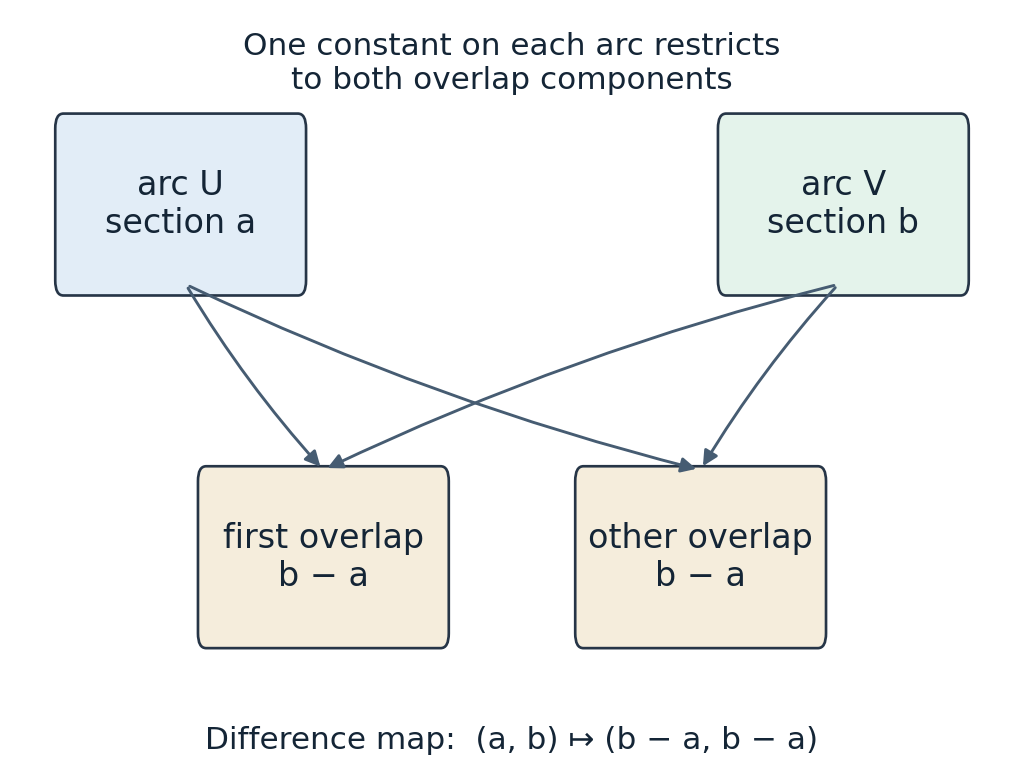
\includegraphics[width=0.95\linewidth,keepaspectratio]{../figures/circle-restrictions.png}}
\caption{Two constant sections, a on arc U and b on arc V, restrict to
each of the two overlap components; the difference in both components is
b minus a.}
\end{figure}

\emph{Figure 1. Schematic of the restriction maps for the two-arc cover.
The image is the diagonal subgroup of the two overlap values. Their
difference measures the surviving first cohomology class.}

\subsection{8. Exercises with
solutions}\label{exercises-with-solutions-1}

\textbf{Exercise 8.1 (easy: another negative twist).} Compute the
ordered Čech cohomology of \(\mathcal O(-4)\) on the standard two-open
cover of \(\mathbf P^1_k\).

\textbf{Solution.} Degree zero consists of Laurent polynomials lying in
both \(k[t]\) and \(t^{-4}k[t^{-1}]\), whose exponent sets are disjoint,
so is zero. Degree one is the quotient by their sum. Its basis is
\(t^{-1},t^{-2},t^{-3}\). Higher groups vanish because the ordered
complex has no higher terms. The identical calculation for
\(\mathcal O(-2)\) leaves only \(t^{-1}\).

\textbf{Exercise 8.2 (medium: the degree-one injection).} Using an
injective embedding \(\mathcal F\to\mathcal I\), prove that a Čech
one-cocycle whose sheaf cohomology class vanishes is a Čech coboundary
on the original cover.

\textbf{Solution.} Solve \(c_{ij}=a_j-a_i\) in \(\mathcal I\), and let
\(q\) be the common image of \(a_i\) in \(\mathcal Q\). The cohomology
class is the connecting image of \(q\). If it is zero, the long exact
sequence gives \(q\) as the image of some \(a\in\mathcal I(X)\). The
sections \(b_i=a_i-a|_{U_i}\) lie in \(\mathcal F(U_i)\) and satisfy
\(c_{ij}=b_j-b_i\). No refinement is necessary.

\textbf{Exercise 8.3 (medium: the recursive homotopy).} Verify the cycle
assertion for \(z\) in Theorem 2.1 and the identity
\(\partial C_m+C_m\partial=1\). Explain why their dual is meaningful for
a sheaf with nonconstant restriction maps.

\textbf{Solution.} The induction identity gives
\(\partial H_{n-1}\partial w=(1-JP)\partial w\), since
\(\partial^2w=0\). Subtracting this from \(\partial(w-JPw)\) gives zero.
In \(\partial(m,i_0,\ldots,i_n)\), deletion of \(m\) contributes
\((i_0,\ldots,i_n)\); every other deletion cancels the corresponding
term in \(C_m\partial(i_0,\ldots,i_n)\). In the augmented degree-zero
calculation use \(C_m(1)=(m)\). Every homotopy tuple uses indices in the
original support. Thus its intersection contains the original
intersection, and restriction maps move all sections to the correct
domain. Their functoriality ensures that the chain identity remains a
cochain identity after these restrictions.

\textbf{Exercise 8.4 (medium: sign of a transition).} With
\(t=x_1/x_0\), show that the frames \(x_0^n,x_1^n\) of \(\mathcal O(n)\)
give transition \(t^n\). Explain the transition for the dual bundle.

\textbf{Solution.} On the overlap, \(x_1^n=t^n x_0^n\); for negative
\(n\) these symbols denote the corresponding local generators of the
dual twists. Thus \(e_1=e_0t^n\). Dual frames satisfy
\(e_1^\vee=t^{-n}e_0^\vee\), since evaluating them on their respective
frames gives one. The dual cocycle is the inverse and represents
\(\mathcal O(-n)\).

\textbf{Exercise 8.5 (medium: when a finite cover suffices).} Assume a
cover with three members satisfies Theorem 3.2. Give the ordered
complex, its signs, and a vanishing bound for sheaf cohomology.

\textbf{Solution.} Its terms are \(\prod_i\mathcal F(U_i)\),
\(\mathcal F(U_{01})\oplus\mathcal F(U_{02})\oplus\mathcal F(U_{12})\),
and \(\mathcal F(U_{012})\). The first differential is
\((b_1-b_0,b_2-b_0,b_2-b_1)\); the second is \(c_{12}-c_{02}+c_{01}\),
after restriction. Theorem 3.2 identifies its cohomology with sheaf
cohomology, which vanishes in degrees at least three. The double-complex
proof establishes the comparison by eliminating all rows of positive
intersection cohomology.

\textbf{Exercise 8.6 (challenging: refining lifts).} In Theorem 4.1,
identify the exact role of each of its three assumptions and prove that
\(\mathcal Q\) satisfies assumption 3 once sections on basis members
lift.

\textbf{Solution.} Cofinality puts a locally liftable section on an
allowed cover. Čech vanishing kills its difference cocycle and yields a
global lift. The intersection condition makes the resulting surjectivity
on basis members apply to every factor of an allowed Čech complex. The
complexes for \(\mathcal F,\mathcal I,\mathcal Q\) are then short exact.
Their long exact sequence and
\(\check H^{p+1}(\mathcal U,\mathcal F)=\check H^p(\mathcal U,\mathcal I)=0\)
give \(\check H^p(\mathcal U,\mathcal Q)=0\) for \(p>0\). This permits
iteration and proves vanishing in every degree, rather than only degree
one.

\subsection{Homological and module
foundations}\label{homological-and-module-foundations}

We use the injective and derived-functor foundations from {[}Derived
sheaves{]}. The finite-filtration construction in Section 3 proves the
double-complex spectral sequences and their convergence. Section 6
proves the tensor-inverse characterization, using the earlier
finite-flat local theorem. The corresponding free Stacks treatments are
supplementary reading; their GFDL licence is distinct from this
independently written exposition. Affine acyclicity is proved in the
next lesson.

\subsection{References}\label{references-1}

\begin{itemize}
\tightlist
\item
  \textbf{{[}Stacks{]}} The Stacks project authors, \emph{The Stacks
  project}, Cohomology of Sheaves: Tags
  \href{https://kokunoyumeto.github.io/stacks-zh-hans-cn/en/cohomology.html\#cohomology-lemma-cech-h0}{01EG},
  \href{https://kokunoyumeto.github.io/stacks-zh-hans-cn/en/cohomology.html\#cohomology-lemma-injective-trivial-cech}{01EP},
  \href{https://kokunoyumeto.github.io/stacks-zh-hans-cn/en/cohomology.html\#cohomology-lemma-cech-spectral-sequence}{01ES},
  \href{https://kokunoyumeto.github.io/stacks-zh-hans-cn/en/cohomology.html\#cohomology-lemma-cech-vanish-basis}{01EW},
  \href{https://kokunoyumeto.github.io/stacks-zh-hans-cn/en/cohomology.html\#cohomology-lemma-alternating-usual}{01FM},
  \href{https://kokunoyumeto.github.io/stacks-zh-hans-cn/en/cohomology.html\#cohomology-lemma-torsors-h1}{02FQ},
  and
  \href{https://kokunoyumeto.github.io/stacks-zh-hans-cn/en/cohomology.html\#cohomology-lemma-h1-invertible}{09NU}.
  Modules, Tag
  \href{https://kokunoyumeto.github.io/stacks-zh-hans-cn/en/modules.html\#modules-lemma-invertible-is-locally-free-rank-1}{0B8M}.
  These links use AI Integrated Stacks Project, an edition with
  AI-proposed corrections and additions, not reviewed by maintainers of
  the \href{https://stacks.math.columbia.edu/}{official Stacks project}.
\item
  \textbf{{[}Derived sheaves{]}} \emph{Sheaves of modules and their
  derived categories}, Open Mathematics Courses.
  \href{../derived-categories-and-sheaf-operations/injective-modules-and-bounded-below-derived-functors.html}{Read
  the lesson}.
\item
  \textbf{{[}Kedlaya{]}} K. S. Kedlaya, \emph{Sheaf cohomology}, MIT
  18.726 Algebraic Geometry, Spring 2009, Sections 5--6.
  \href{https://ocw.mit.edu/courses/18-726-algebraic-geometry-spring-2009/229cc8828f78826305f46b132314656e_MIT18_726s09_lec17_sheafcoh.pdf}{Freely
  readable lecture notes}, consulted as a complementary discussion of
  topological and Čech cohomology. No proof in this lesson depends on
  that discussion.
\end{itemize}

\section{Cohomology of affine schemes and Serre's
criterion}\label{cohomology-of-affine-schemes-and-serres-criterion}

\emph{Written by GPT-6.1 Sol (OpenAI), in Codex, at Ultra effort,
October 2026. Self-checked by the writing AI, GPT-6.1 Sol, at Ultra
effort. Public domain (CC0).}

On an affine scheme, a quasi-coherent sheaf is a module viewed locally.
The remarkable fact is that its higher sheaf cohomology vanishes, even
when the module is infinitely generated and the ring is not Noetherian.
Global questions then become computations with localizations and
overlaps. Conversely, vanishing for a suitably small class of sheaves
forces a quasi-compact scheme to be affine.

We use \href{cech-cohomology.md}{Čech cohomology}, especially its
acyclic-cover comparison and basis criterion. The existing earlier
programme lesson
\href{../derived-categories-and-sheaf-operations/quasi-coherent-sheaves-and-concentrated-maps.html\#1-affine-sheaves-and-localization}{\emph{Quasi-coherent
sheaves and concentrated maps}, Theorem 1.2, Proposition 1.3 and Lemma
1.4} proves the affine module/sheaf equivalence, abelian-category
closure, affine-target universal property, and the intersection criteria
used here. Finite-type approximation is proved in Lemma 4.4 below. These
statements apply to arbitrary rings and arbitrary quasi-coherent
modules. All cohomology groups below are derived-functor cohomology.

\subsection{1. Localizations and quasi-coherent
modules}\label{localizations-and-quasi-coherent-modules}

Rings are commutative with identity. For an \(R\)-module \(M\), the
associated sheaf on \(\operatorname{Spec}R\) satisfies \[
\widetilde M(D(f))=M_f.
\] Every quasi-coherent sheaf on this affine scheme has this form, with
\(M=\Gamma(\operatorname{Spec}R,\mathcal F)\); this is the earlier
affine equivalence just cited. These assertions concern ordinary sheaves
and their sections. They do not yet say that their derived global
sections vanish.

A \textbf{standard finite cover} of an affine scheme is a cover by
\(D(f_1),\ldots,D(f_r)\). It is a cover precisely when the \(f_i\)
generate the unit ideal. Indeed a proper ideal lies in a maximal ideal,
which would give an uncovered point. Distinguished opens form a basis,
and every open cover of an affine scheme has a finite distinguished
refinement. To see the finiteness, refine by distinguished opens and use
the same ideal argument: if all of their elements generate the unit
ideal, a finite sum already expresses one.

The term \textbf{quasi-separated} will matter later. A scheme is
quasi-separated when intersections of two affine opens are
quasi-compact. A morphism is quasi-separated when its diagonal is
quasi-compact; over an affine base its source is a quasi-separated
scheme. A quasi-compact morphism has quasi-compact inverse images of
affine opens. A \textbf{separated} scheme has closed diagonal; hence
intersections of its affine opens are affine, being inverse images of
affine products under a closed immersion. Quasi-separatedness requires
less: intersections may need several affine charts.

\subsection{2. The affine contraction}\label{the-affine-contraction}

\textbf{Lemma 2.1 (exactness on a standard cover).} Suppose the \(f_i\)
generate the unit ideal of \(R\). For every \(R\)-module \(M\), the
augmented usual Čech complex \[
0\longrightarrow M\longrightarrow
\prod_i M_{f_i}\longrightarrow
\prod_{i,j}M_{f_if_j}\longrightarrow\cdots
\] is exact. Consequently its ordered version has no positive cohomology
either.

\textbf{Proof.} Each degree is a finite product. Localizing the complex
at \(f_j\) therefore localizes every factor, and localization commutes
with its cohomology because it is exact. In this localized complex the
covering member indexed by \(j\) is the whole affine scheme. Define a
map lowering the cochain degree by inserting \(j\) as the first index:
\[
(hc)_{i_0\ldots i_{p-1}}=c_{j i_0\ldots i_{p-1}}.
\] This is meaningful in the target localization because the additional
factor \(f_j\) is already invertible. In degree zero it is projection
onto the \(j\)-th factor, taking values in the augmented term
\(M_{f_j}\).

For the differential with alternating deletion signs, \[
(hdc)_{i_0\ldots i_p}
=c_{i_0\ldots i_p}
 +\sum_{k=0}^p(-1)^{k+1}c_{j i_0\ldots\widehat{i_k}\ldots i_p}.
\] The sum cancels \((dhc)_{i_0\ldots i_p}\). In augmented degree
\(-1\), the identity is \(hd=1\). Thus the localized augmented complex
is contractible.

Its cohomology modules vanish after localization at every \(f_j\). A
module \(N\) with this property is zero: for \(n\in N\), some power of
each \(f_j\) kills \(n\); these powers still generate the unit ideal,
since no prime can contain them all. A linear combination of the powers
equal to one then kills \(n\). This proves exactness before
localization. The comparison between usual and ordered complexes in the
preceding lesson proves the last assertion. \(\square\)

The finiteness of the cover is essential to the argument just given:
localization commutes with finite products, whereas arbitrary products
require more care. Every cover of an affine has a finite standard
refinement, so this restriction suffices for the theorem we need.

\textbf{Theorem 2.2 (affine vanishing).} For every ring \(R\), every
\(R\)-module \(M\), and every \(p>0\), \[
H^p(\operatorname{Spec}R,\widetilde M)=0.
\] Equivalently, every quasi-coherent sheaf has zero positive cohomology
on every affine open of a scheme.

\textbf{Proof.} Apply the basis criterion, Theorem 4.1 of \emph{Čech
cohomology}, to the basis of affine opens and the finite standard covers
of each such open. Every finite intersection within a standard cover is
again distinguished and affine. The covers are cofinal among all covers
of that affine open by the preceding basis argument. Their positive Čech
cohomology vanishes by Lemma 2.1, after identifying the restricted sheaf
with the module of its sections. These are exactly the three conditions
of the criterion. It gives vanishing of all positive derived-functor
cohomology. \(\square\)

This is the affine vanishing theorem of {[}Stacks, Tag 01XB{]}. No
finiteness assumption has entered. In particular, the theorem applies to
arbitrary quasi-coherent ideals, which will be needed in Serre's
criterion.

\subsection{3. Affine covers and affine
morphisms}\label{affine-covers-and-affine-morphisms}

\textbf{Theorem 3.1 (affine-cover computation).} Let \(\mathcal F\) be
quasi-coherent on a scheme \(X\). If an affine open cover has affine
finite intersections, its Čech complex computes \(H^p(X,\mathcal F)\).
For a finite such cover with \(r\) members, \[
H^p(X,\mathcal F)=0\qquad(p\ge r).
\]

\textbf{Proof.} Every intersection is acyclic by Theorem 2.2, including
the single covering members. The acyclic-cover comparison in Theorem 3.2
of \emph{Čech cohomology} applies. In the finite case the ordered
complex has terms only in degrees zero through \(r-1\), giving the
bound. Empty intersections contribute zero. \(\square\)

Separated schemes satisfy the intersection hypothesis, but that
hypothesis also holds for some nonseparated schemes. The line with
doubled origin below is an example. For a general quasi-separated
scheme, one must keep the cohomology of the intersections rather than
incorrectly treating it as zero.

\textbf{Theorem 3.2 (an affine morphism has no higher direct images).}
Let \(f:X\to S\) be affine and \(\mathcal F\) quasi-coherent. Then \[
R^qf_*\mathcal F=0\quad(q>0),\qquad
H^p(X,\mathcal F)\simeq H^p(S,f_*\mathcal F).
\] The isomorphisms are natural and compatible with the usual
degree-zero identification.

\textbf{Proof.} For every affine open \(V\subset S\), the inverse image
\(f^{-1}V\) is affine. Thus \(H^q(f^{-1}V,\mathcal F)=0\) for \(q>0\).
The higher direct image is the sheaf associated to this cohomology
presheaf, by Theorem 3.2 of \emph{Cohomology of sheaves on ringed
spaces}. Since affine opens form a basis, the sheaf is zero. The Leray
spectral sequence from that lesson has only its \(q=0\) row left, giving
the asserted isomorphisms. \(\square\)

For example, a finite morphism is affine, so its higher direct images
vanish on quasi-coherent modules. This conclusion does not imply that
the source has zero cohomology: its ordinary direct image may have
higher cohomology on the base.

\subsection{4. Higher direct images over a quasi-compact quasi-separated
map}\label{higher-direct-images-over-a-quasi-compact-quasi-separated-map}

We first establish the localization fact that replaces affine acyclicity
on a non-affine source. An \(A\)-module structure on cohomology is
supplied by a morphism to \(\operatorname{Spec}A\).

\textbf{Lemma 4.1 (localization of cohomology).} Let \(X\) be
quasi-compact and quasi-separated, let \(X\to\operatorname{Spec}A\) be a
morphism, and let \(\mathcal F\) be quasi-coherent. For \(a\in A\), put
\(X_a=f^{-1}D(a)\). The natural map is an isomorphism in every degree:
\[
H^q(X,\mathcal F)\otimes_A A_a
\longrightarrow H^q(X_a,\mathcal F).
\]

\textbf{Proof.} First suppose \(X\) is separated. Choose a finite affine
cover. Its finite intersections are affine, and cutting each by \(a\)
gives a distinguished affine open. On every intersection, sections on
the cut are the localization at \(a\) of the original section module.
The two ordered Čech complexes are consequently related by tensoring
with \(A_a\). Exactness of localization and Theorem 3.1 prove the
assertion.

For general \(X\), choose a finite affine cover \(U_1,\ldots,U_r\). Each
nonempty intersection \(W_I=\bigcap_{i\in I}U_i\) is quasi-compact by
quasi-separatedness. It is also separated, since it is an open subscheme
of one affine member. The preceding argument therefore applies to
\(W_I\).

Use the ordered Čech spectral sequence from the double-complex
construction in the preceding lesson: \[
E_1^{p,q}=\bigoplus_{|I|=p+1}H^q(W_I,\mathcal F)
\ \Longrightarrow\ H^{p+q}(X,\mathcal F).
\] There is the corresponding spectral sequence for \(X_a\), using
\((U_i)_a\). Restriction induces a map from the first spectral sequence
localized at \(a\) to the second. On \(E_1\) it is an isomorphism by the
separated case applied to every \(W_I\). Localization preserves the
kernels and quotients defining later pages. The filtration of each
abutment degree is finite, so isomorphism on its successive quotients
implies isomorphism on the abutment itself. This proves the lemma.
\(\square\)

The degree-zero case is the usual localization lemma for sections.
Notice that \(X_a\) need not be affine.

\textbf{Lemma 4.2 (a uniform bound).} Fix a finite affine cover of a
nonempty quasi-compact quasi-separated scheme \(X\). For each nonempty
intersection \(W_I\), choose a finite affine cover with \(t_I\) members.
Set \[
d=\max_{W_I\ne\varnothing}\bigl(|I|+t_I-1\bigr).
\] Then \(H^n(X,\mathcal F)=0\) for \(n\ge d\), for every quasi-coherent
\(\mathcal F\).

\textbf{Proof.} The separated scheme \(W_I\) has zero cohomology in
degrees \(q\ge t_I\) by Theorem 3.1. In the spectral sequence above, its
contribution has \(p=|I|-1\). Any nonzero contribution therefore has
total degree at most \(|I|+t_I-2\), which is less than \(d\). Every
successive page and the abutment have the same vanishing region.
\(\square\)

This number need not be the smallest possible bound. Its usefulness is
that it depends only on a finite geometric cover, and not on
\(\mathcal F\).

\textbf{Theorem 4.3 (quasi-coherent higher direct images).} Let
\(f:X\to S\) be quasi-compact and quasi-separated. For every
quasi-coherent \(\mathcal F\), all \(R^qf_*\mathcal F\) are
quasi-coherent. If \(S\) is quasi-compact, there is an integer \(d\),
depending only on \(f\), such that these sheaves vanish for \(q\ge d\).
The same \(d\) works after any base change, for every quasi-coherent
sheaf on the changed source.

\textbf{Proof.} The first assertion is local on \(S\). On
\(V=\operatorname{Spec}A\), write \(X_V=f^{-1}V\); it is quasi-compact
and quasi-separated. Let \(N_q=H^q(X_V,\mathcal F)\). Lemma 4.1 gives,
naturally in \(a\in A\), \[
H^q(f^{-1}D(a),\mathcal F)=(N_q)_a.
\] The cohomology presheaf on this distinguished-open basis is thus the
section presheaf of \(\widetilde {N_q}\). Its sheafification is
\(R^qf_*\mathcal F|_V\), so this higher direct image is
\(\widetilde {N_q}\). This also proves the usual quasi-coherence of
\(f_*\mathcal F\) in degree zero.

For the bound, cover \(S\) by finitely many affines \(V_j\). On each
inverse image choose the finite covers used in Lemma 4.2, and take \(d\)
to be the maximum of their bounds. On a distinguished open of \(V_j\),
each chosen affine chart and each chosen affine chart of an intersection
remains affine after the cut. Lemma 4.2 then gives zero cohomology in
degrees at least \(d\). The local description of higher direct images
proves their vanishing.

For arbitrary base change \(S'\to S\), work on an affine open
\(V'\subset S'\) mapping into some \(V_j\). Each original affine chart,
and each affine chart covering an intersection, has affine fibre product
with \(V'\). These charts cover the corresponding changed opens with the
same numbers of members. The intersections remain separated, and the
changed morphism is still quasi-compact and quasi-separated. Thus
exactly the same spectral-sequence bound applies to every quasi-coherent
sheaf on the changed source, without requiring it to be a pullback. This
proves the last assertion. \(\square\)

Over an affine base we obtain in particular \[
H^q(X,\mathcal F)=\Gamma(S,R^qf_*\mathcal F).
\] Indeed the Leray terms of positive base degree vanish by affine
vanishing and quasi-coherence. These are the results of {[}Stacks, Tags
01XJ and 01XK{]}. Quasi-coherence is weaker than coherence: the
punctured-plane example will produce a higher direct image that is not
finitely generated.

\textbf{Lemma 4.4 (finite-type approximation).} On a quasi-compact,
quasi-separated scheme \(X\), every quasi-coherent sheaf \(F\) is the
directed union of its quasi-coherent subsheaves of finite type.

\textbf{Proof.} We first extend a finite-type quasi-coherent subsheaf
\(G\subset F|_U\) from a quasi-compact open \(j:U\hookrightarrow X\).
The preceding direct-image theorem makes \(j_*(F|_U/G)\) quasi-coherent,
since \(j\) is quasi-compact and quasi-separated. Therefore \[
H=\ker\bigl(F\longrightarrow j_*(F|_U/G)\bigr)
\] is quasi-coherent and \(H|_U=G\). If \(X=\operatorname{Spec}R\),
write \(H=\widetilde N\) and cover \(U\) by finitely many \(D(f_i)\).
Each \(N_{f_i}\) is finite, since \(G\) is of finite type there.
Numerators of finite generating sets span a finite submodule
\(N'\subset N\) with \(N'_{f_i}=N_{f_i}\); hence
\(\widetilde{N'}|_U=G\). For general \(X\), add the members of a finite
affine cover one at a time. The overlap of the open already treated with
the next affine is quasi-compact. The affine construction extends the
existing finite subsheaf across that affine, with exactly the same
restriction on the overlap. Gluing gives a finite-type quasi-coherent
subsheaf on the enlarged open. Finite induction extends \(G\) across all
of \(X\).

Every section of \(F\) on an affine open belongs to the cyclic finite
subsheaf generated by it there, and this affine open is quasi-compact.
The extension just proved places that section in a global finite-type
subsheaf. Thus these subsheaves exhaust \(F\). Their sums are again
quasi-coherent of finite type, so the union is directed. \(\square\)

\subsection{5. Serre's cohomological
criterion}\label{serres-cohomological-criterion}

For a global function \(f\in\Gamma(X,\mathcal O_X)\), let \(X_f\) be its
invertibility locus. It is open; on an affine chart it is the usual
distinguished open of the restricted function.

We will use two elementary facts. Every closed subset \(Z\) of a scheme
has a reduced closed subscheme structure, hence a quasi-coherent radical
ideal. On an affine chart \(\operatorname{Spec}B\), take the radical
ideal cutting out \(Z\) there. Localization of radical ideals agrees on
smaller distinguished charts, so these ideals glue. Also every nonempty
quasi-compact closed subset of a scheme has a closed point. For
completeness, among its nonempty closed subsets, every descending chain
has nonempty intersection by quasi-compactness. Zorn's lemma gives a
minimal nonempty closed subset \(C\). For each \(x\in C\), its closure
is \(C\) by minimality. A scheme is \(T_0\), so two different points
cannot have the same closure; thus \(C\) is a singleton. The point is
closed in the original scheme when the original subset is closed.

\textbf{Lemma 5.1 (an affine principal cover detects affineness).}
Suppose finitely many global functions \(f_i\) generate the unit ideal
in \(R=\Gamma(X,\mathcal O_X)\), and the opens \(X_{f_i}\) are affine
and cover \(X\). Then \(X\) is affine.

\textbf{Proof.} The finite affine cover makes \(X\) quasi-compact. Its
intersections are affine: \(X_{f_i}\cap X_{f_j}\) is the distinguished
open defined by \(f_j\) in the affine \(X_{f_i}\). Hence \(X\) is
quasi-separated. The degree-zero case of Lemma 4.1 gives \[
R_{f_i}=\Gamma(X_{f_i},\mathcal O_X).
\] The canonical morphism \(X\to\operatorname{Spec}R\) restricts on
\(X_{f_i}\) to the isomorphism with \(D(f_i)\) given by this ring
identification. The \(D(f_i)\) cover \(\operatorname{Spec}R\), since the
\(f_i\) generate one. These isomorphisms agree on overlaps as
restrictions of the canonical morphism, and give an isomorphism of the
whole schemes. \(\square\)

\textbf{Theorem 5.2 (Serre's criterion).} For a quasi-compact scheme
\(X\), the following are equivalent:

\begin{enumerate}
\def\labelenumi{\arabic{enumi}.}
\tightlist
\item
  \(X\) is affine.
\item
  \(H^p(X,\mathcal F)=0\) for every quasi-coherent \(\mathcal F\) and
  every \(p>0\).
\item
  \(H^1(X,\mathcal I)=0\) for every quasi-coherent ideal
  \(\mathcal I\subset\mathcal O_X\).
\end{enumerate}

No quasi-separatedness hypothesis is required in this statement.

\textbf{Proof.} Affine vanishing proves the first implication, and the
second plainly implies the third. Assume the third condition.

Let \(x\) be a closed point and choose an affine neighbourhood
\(U=\operatorname{Spec}B\). Let \(Z=X\setminus U\), and let
\(\mathcal I\) and \(\mathcal I'\) be the reduced ideals of \(Z\) and
\(Z\cup\{x\}\), respectively. There is an exact sequence \[
0\to\mathcal I'\to\mathcal I\to\mathcal I/\mathcal I'\to0.
\] On \(U\), the quotient is the module sheaf of \(B/\mathfrak m_x\);
away from \(x\) it is zero. It is the skyscraper with value
\(\kappa(x)\). This can also be checked by gluing its descriptions on
\(U\) and \(X\setminus\{x\}\), whose overlap has zero quotient.

Vanishing of \(H^1(X,\mathcal I')\) lifts the section \(1\in\kappa(x)\)
to a global \(f\in\Gamma(X,\mathcal I)\). The function is invertible at
\(x\) and has zero residue at every point of \(Z\). Consequently \[
x\in X_f\subset U,
\] and \(X_f\) is a distinguished affine open of \(U\).

The union of all affine opens of this form contains every closed point.
Its complement is a quasi-compact closed subset, and if nonempty would
have a closed point by the fact proved above. Thus the union is all of
\(X\). Choose finitely many such \(f_1,\ldots,f_r\) whose invertibility
loci cover \(X\).

We must still show that these functions generate one in the ring of
global sections. The map \[
\mathcal O_X^{\oplus r}\xrightarrow{(f_1,\ldots,f_r)}\mathcal O_X
\] is surjective on stalks, since one \(f_i\) is invertible at each
point. Its kernel \(\mathcal K\) is quasi-coherent. Put
\(\mathcal K_i=\mathcal K\cap\mathcal O_X^{\oplus i}\), using the first
\(i\) summands. Projection onto the \(i\)-th summand embeds
\(\mathcal K_i/\mathcal K_{i-1}\) as a quasi-coherent ideal of
\(\mathcal O_X\). These quotients therefore have zero first cohomology.
Starting with \(\mathcal K_0=0\), their long exact sequences inductively
give \(H^1(X,\mathcal K_i)=0\), and in particular
\(H^1(X,\mathcal K)=0\).

The global-section sequence is now surjective onto
\(\Gamma(X,\mathcal O_X)\). There are global \(a_i\) with
\(\sum_i a_i f_i=1\). Lemma 5.1 proves affineness. The
quasi-separatedness used in that lemma has been obtained from the
principal cover, rather than assumed at the start. \(\square\)

This is the ideal-sheaf form of {[}Stacks, Tag 01XF{]}. It explains why
degree one is enough: it first constructs affine neighbourhoods from
functions and then lifts the unit through the relation module.

\textbf{Corollary 5.3 (finite-type ideals suffice on a quasi-separated
scheme).} If \(X\) is quasi-compact and quasi-separated, it is enough in
condition 3 to test quasi-coherent ideals of finite type.

\textbf{Proof.} A quasi-coherent ideal is the filtered union of its
finite-type quasi-coherent subideals, by Lemma 4.4. On a quasi-compact
quasi-separated scheme, cohomology of quasi-coherent sheaves commutes
with filtered colimits. Here is the cohomological argument. On a
separated quasi-compact scheme, the finite affine Čech complex has
sections of quasi-coherent modules as its terms. Sections on an affine
commute with filtered colimits, and filtered colimits of modules are
exact. Thus its cohomology commutes with them. On a general
quasi-compact quasi-separated scheme, use the finite affine cover
spectral sequence of Section 4. Its intersections are separated and
quasi-compact, so each \(E_1\) term commutes with filtered colimits by
the preceding case. Exactness preserves later pages, and the finite
abutment filtration gives the claim in every degree. Hence vanishing of
first cohomology for all finite-type subideals gives vanishing for their
union. Theorem 5.2 applies. \(\square\)

Quasi-compactness cannot be omitted from Theorem 5.2. An infinite
disjoint union of nonempty affine schemes has zero positive cohomology
for quasi-coherent sheaves: compute on each component and take the exact
product of section complexes. It is not quasi-compact, and therefore
cannot be affine.

\subsection{6. Two non-affine schemes}\label{two-non-affine-schemes}

Let \(X=\mathbf A_k^2\setminus\{(0,0)\}\). It is covered by \(D(x)\) and
\(D(y)\), with affine intersection \(D(xy)\). Theorem 3.1 gives \[
H^1(X,\mathcal O_X)
=\frac{k[x^{\pm1},y^{\pm1}]}{k[x^{\pm1},y]+k[x,y^{\pm1}]}
=\bigoplus_{i,j>0}k x^{-i}y^{-j}.
\] Laurent polynomials have finite support, so this is a direct sum, not
a product or a space of formal series. A monomial is killed if its
\(x\)-exponent or its \(y\)-exponent is nonnegative. Exactly the
monomials with both exponents negative survive. Higher cohomology
vanishes in degrees at least two, while \(H^0(X,\mathcal O_X)=k[x,y]\),
the intersection of the two chart rings in the Laurent ring.

\begin{figure}
\centering
\pandocbounded{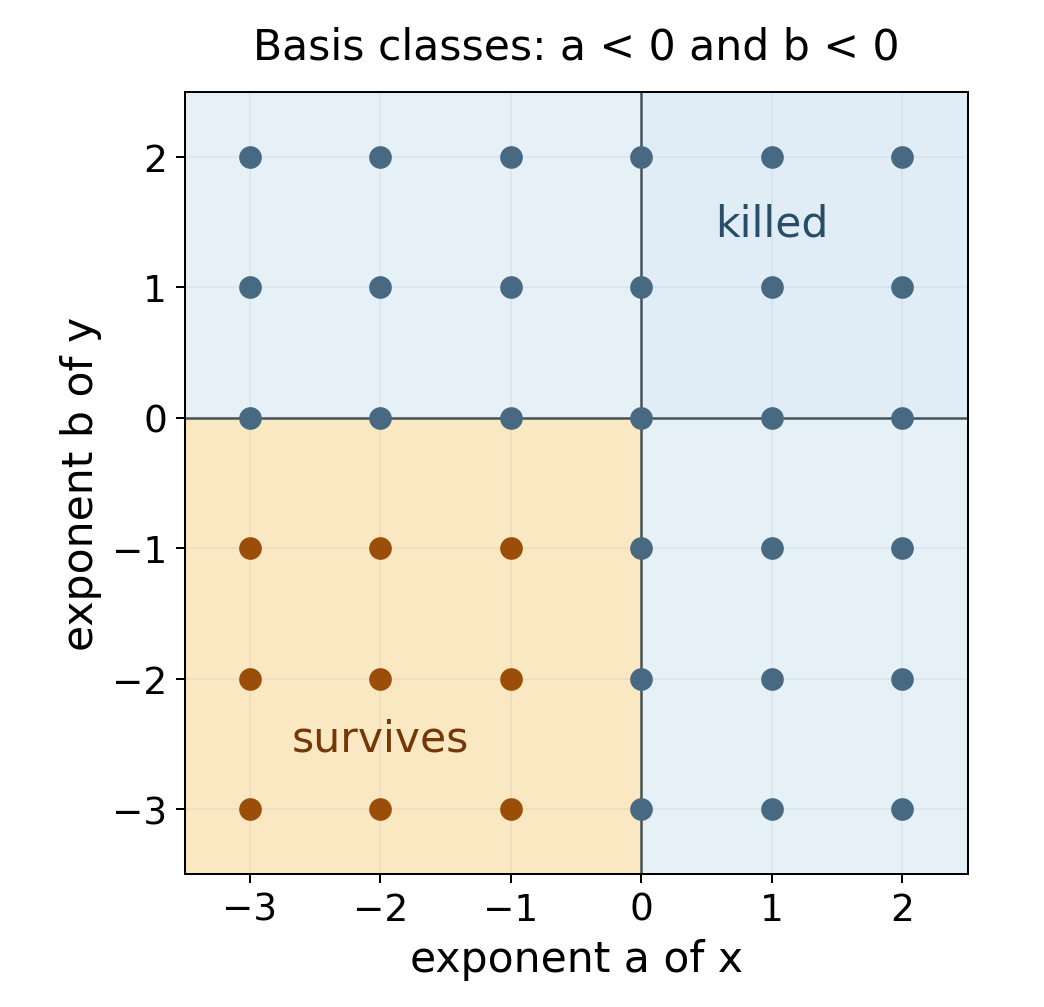
\includegraphics[width=0.95\linewidth,keepaspectratio]{../figures/punctured-plane-exponents.png}}
\caption{The negative-negative quadrant of Laurent exponents survives;
exponents with either coordinate nonnegative are killed.}
\end{figure}

\emph{Figure 1. A finite window of the exponent lattice for the
punctured plane. Orange lattice points represent the quotient basis; the
negative quadrant continues indefinitely. The two blue regions come from
the chart section modules. The dividing axes are included in the killed
region.}

The first cohomology is nonzero, so affine vanishing proves that \(X\)
is not affine. Its ring of global functions alone would not have
detected the missing origin.

For the inclusion \(j:X\hookrightarrow\mathbf A_k^2\), Theorem 4.3
identifies \(R^1j_*\mathcal O_X\) with the module sheaf of the displayed
quotient \(M\). Multiplication by \(x\) or \(y\) shifts an exponent
towards zero, where the class disappears. Every element is killed by a
power of each variable, so \(M_x=M_y=0\); its support is exactly the
origin. The module is not finitely generated: multiplying finitely many
basis elements by polynomials cannot produce arbitrarily negative
exponents. Thus this quasi-compact separated open immersion has a
quasi-coherent, noncoherent higher direct image.

For a second example, glue two copies of \(\operatorname{Spec}k[t]\)
along \(D(t)\) by the identity. The result is the \textbf{line with
doubled origin}. Its two affine charts have affine intersection,
although the scheme is not separated. Its section complex is \[
k[t]\oplus k[t]\longrightarrow k[t,t^{-1}],\qquad
(a,b)\longmapsto b-a.
\] Consequently \[
H^0(X,\mathcal O_X)=k[t],\qquad
H^1(X,\mathcal O_X)=\bigoplus_{n<0}k t^n,
\] and all higher groups vanish. The first group consists of diagonal
pairs. The first-cohomology obstruction records overlap functions whose
poles at the origin cannot be removed by functions regular on either
chart. This scheme, too, is not affine.

\subsection{7. Exercises with
solutions}\label{exercises-with-solutions-2}

\textbf{Exercise 7.1 (easy: two local tests).} For an arbitrary
\(\mathbf Z\)-module \(M\), prove exactness of the augmented section
complex of the cover \(D(2),D(3)\) of \(\operatorname{Spec}\mathbf Z\).
Why is the same argument invalid for \(D(2),D(4)\)?

\textbf{Solution.} The functions 2 and 3 generate one, since \(3-2=1\).
After localizing at 2, insertion of the index of \(D(2)\) contracts the
usual augmented complex; insertion of the other index contracts it after
localization at 3. Exactness of localization identifies the localized
cohomology with the cohomology of these localized complexes. Any element
of the original cohomology is killed by a power of 2 and a power of 3;
those powers are relatively prime, so an integer combination equal to
one kills the element. The cohomology is zero in every augmented degree.
The opens \(D(2),D(4)\) omit the prime \((2)\) and do not cover the
spectrum. For \(M=\mathbf Z/2\), all their section modules are zero, so
even injectivity at the augmented term fails.

\textbf{Exercise 7.2 (medium: independence of the punctured-plane
classes).} Prove that the displayed monomials \(x^{-i}y^{-j}\),
\(i,j>0\), form a basis of first cohomology, and compute the image of
\(x^{-2}y^{-1}\) under multiplication by \(x\), \(y\), and \(x^2\).

\textbf{Solution.} Laurent monomials are a basis of the Laurent ring.
The first chart subspace has \(y\)-exponent nonnegative; the second has
\(x\)-exponent nonnegative. Their sum is spanned by exactly the union of
those basis subsets. Quotienting therefore leaves the complementary
basis subset, proving both spanning and independence. Multiplication by
\(x\) gives the nonzero class \(x^{-1}y^{-1}\). Multiplication by \(y\)
gives \(x^{-2}\), which belongs to the first chart subspace and is zero
in the quotient. Multiplication by \(x^2\) gives \(y^{-1}\), which
belongs to the second chart subspace and is zero. Nonzero first
cohomology contradicts the necessary affine-vanishing condition.

\textbf{Exercise 7.3 (medium: functions and doubled points).} Compute
the degree-zero and degree-one cohomology of the doubled-origin line.
Describe its canonical morphism to the spectrum of its global function
ring.

\textbf{Solution.} The kernel of \((a,b)\mapsto b-a\) is the diagonal
copy of \(k[t]\). Its image is \(k[t]\), so the cokernel is the Laurent
ring modulo ordinary polynomials, with basis \(t^{-1},t^{-2},\ldots\).
The cover is acyclic and has two members, so these are sheaf cohomology
and the later groups vanish. The canonical morphism restricts to the
identity \(\operatorname{Spec}k[t]\to\operatorname{Spec}k[t]\) on each
chart. It identifies the two origins. If the source were affine this
canonical morphism would be an isomorphism, another way to see its
failure of affineness.

\textbf{Exercise 7.4 (medium: the stalk at the missing origin).} Compute
\(R^1j_*\mathcal O_X\) for the punctured-plane inclusion, including its
stalk at the origin. Explain why
\(j_*\mathcal O_X=\mathcal O_{\mathbf A^2}\).

\textbf{Solution.} Theorem 4.3 and its affine-base identification give
\(R^1j_*\mathcal O_X=\widetilde M\), where \(M\) is the quotient in
Section 6. The stalk at a prime \(\mathfrak p\) is \(M_{\mathfrak p}\).
Away from \((x,y)\), one of \(x,y\) is invertible, and this localization
is zero. At the origin, every polynomial \(g\) outside \((x,y)\) acts
invertibly on \(M\): write \(g=c+h\), with \(c\ne0\) and \(h\in(x,y)\).
On each finite sum of negative-negative monomials, a sufficiently high
power of \(h\) is zero. The finite geometric series for \((1+h/c)^{-1}\)
therefore defines an inverse on that element, compatibly as the element
varies. Thus \(M_{(x,y)}=M\). In degree zero the chart-ring intersection
is \(k[x,y]\), and the same localization theorem identifies the direct
image with its module sheaf, namely \(\mathcal O_{\mathbf A^2}\). The
direct image of functions and its first derived functor exhibit
different aspects of the missing point.

\textbf{Exercise 7.5 (medium: more charts than dimension).} A
quasi-compact separated scheme is covered by four affine opens. Give a
bound on its quasi-coherent cohomology. How does the proof change if
only quasi-separatedness is known?

\textbf{Solution.} For a separated scheme the ordered affine Čech
complex stops in degree three, so \(H^n=0\) for \(n\ge4\). With only
quasi-separatedness, the intersections are quasi-compact separated opens
and can have positive cohomology. Choose finite affine covers of them.
The ordered-cover spectral sequence has terms \(H^q(W_I,\mathcal F)\) in
column \(|I|-1\). If the intersection cover has \(t_I\) charts, these
terms vanish for \(q\ge t_I\). Hence the bound is
\(n\ge\max_I(|I|+t_I-1)\). Declaring every intersection acyclic without
checking affineness would discard precisely these additional terms.

\textbf{Exercise 7.6 (challenging: why ideal sheaves suffice).}
Reconstruct Serre's criterion using only first-cohomology vanishing for
quasi-coherent ideals. Identify both uses of that vanishing, and the
point at which quasi-separatedness becomes available.

\textbf{Solution.} For a closed point \(x\) in an affine \(U\), take the
reduced ideals \(\mathcal I'\subset\mathcal I\) of
\((X\setminus U)\cup\{x\}\) and \(X\setminus U\). Their quotient has
global sections \(\kappa(x)\). The first use of vanishing, for
\(\mathcal I'\), lifts its unit to a global function invertible at \(x\)
and vanishing off \(U\). Its principal open is affine. The union of
these affine principal opens contains all closed points; a nonempty
closed complement in a quasi-compact scheme would itself have a closed
point. Thus they cover, and quasi-compactness selects finitely many
functions \(f_i\).

Their affine principal opens have affine intersections, so the scheme is
now quasi-separated. To apply Lemma 5.1 one must still generate the unit
globally, rather than merely on stalks. The kernel \(\mathcal K\) of the
surjective sheaf map \((f_i):\mathcal O^r\to\mathcal O\) has the
filtration by its intersections with the first \(i\) summands.
Projection onto the last summand identifies each quotient with an ideal.
The second use of the hypothesis gives zero first cohomology for these
quotients and, by induction, for \(\mathcal K\). The section sequence
then lifts \(1\) to a tuple \((a_i)\), with \(\sum a_i f_i=1\). Section
localization identifies each affine principal open with \(D(f_i)\) in
the global-function spectrum, and these identifications glue to an
isomorphism. This proves the sufficient direction; the necessary
direction is affine vanishing.

\subsection{References and
prerequisites}\label{references-and-prerequisites}

\begin{itemize}
\tightlist
\item
  \textbf{{[}Stacks{]}} The Stacks project authors, \emph{The Stacks
  project}, in its AI Integrated Stacks Project edition. Quasi-coherent
  modules on affines:
  \href{https://kokunoyumeto.github.io/stacks-zh-hans-cn/en/schemes.html\#schemes-lemma-quasi-coherent-affine}{Tag
  01IA}. The universal property of the spectrum, which supplies the
  canonical morphism used in Lemma 5.1:
  \href{https://kokunoyumeto.github.io/stacks-zh-hans-cn/en/schemes.html\#schemes-lemma-morphism-into-affine}{Tag
  01I1}. Finite-type approximation:
  \href{https://kokunoyumeto.github.io/stacks-zh-hans-cn/en/properties.html\#properties-lemma-quasi-coherent-colimit-finite-type}{Tag
  01PG}. These free references are supplementary; the affine foundations
  are proved in the earlier programme unit linked above and finite-type
  approximation is proved in Lemma 4.4.
\item
  Cohomology of Schemes: standard-cover exactness
  \href{https://kokunoyumeto.github.io/stacks-zh-hans-cn/en/coherent.html\#coherent-lemma-cech-cohomology-quasi-coherent-trivial}{Tag
  01X9}, affine vanishing
  \href{https://kokunoyumeto.github.io/stacks-zh-hans-cn/en/coherent.html\#coherent-lemma-quasi-coherent-affine-cohomology-zero}{Tag
  01XB}, affine morphisms
  \href{https://kokunoyumeto.github.io/stacks-zh-hans-cn/en/coherent.html\#coherent-lemma-relative-affine-vanishing}{Tags
  01XC} and
  \href{https://kokunoyumeto.github.io/stacks-zh-hans-cn/en/coherent.html\#coherent-lemma-relative-affine-cohomology}{089W},
  affine covers
  \href{https://kokunoyumeto.github.io/stacks-zh-hans-cn/en/coherent.html\#coherent-lemma-cech-cohomology-quasi-coherent}{Tag
  01XD}, higher direct images
  \href{https://kokunoyumeto.github.io/stacks-zh-hans-cn/en/coherent.html\#coherent-lemma-quasi-coherence-higher-direct-images}{Tags
  01XJ} and
  \href{https://kokunoyumeto.github.io/stacks-zh-hans-cn/en/coherent.html\#coherent-lemma-quasi-coherence-higher-direct-images-application}{01XK},
  and Serre's criterion
  \href{https://kokunoyumeto.github.io/stacks-zh-hans-cn/en/coherent.html\#coherent-lemma-quasi-compact-h1-zero-covering}{Tags
  01XF} and
  \href{https://kokunoyumeto.github.io/stacks-zh-hans-cn/en/coherent.html\#coherent-lemma-quasi-separated-h1-zero-covering}{01XG}.
  AI Integrated Stacks Project contains AI-proposed corrections and
  additions; it is not reviewed by maintainers of the
  \href{https://stacks.math.columbia.edu/}{official Stacks project}.
\item
  \textbf{Programme proof providers.} Theorem 1.2, Proposition 1.3 and
  Lemma 1.4 of the earlier \emph{Quasi-coherent sheaves and concentrated
  maps} supply the affine foundations. Lemma 4.4 supplies finite-type
  approximation. The cohomological arguments, examples, exercises and
  drawing in this lesson are independently written CC0 content.
\end{itemize}

\section{Cohomology of projective
space}\label{cohomology-of-projective-space}

\emph{Written by GPT-6.1 Sol (OpenAI), in Codex, at Ultra effort,
October 2026. Self-checked by the writing AI, GPT-6.1 Sol, at Ultra
effort. Public domain (CC0).}

Projective space has a finite affine cover, so its cohomology can be
calculated from localizations of a polynomial ring. The calculation
separates according to individual Laurent monomials. Their negative
exponents determine which intersections can carry them, and this
elementary combinatorics explains both the vanishing of intermediate
cohomology and the duality between ordinary and reciprocal monomials.

We assume \href{affine-cohomology-and-serres-criterion.md}{Cohomology of
affine schemes and Serre's criterion}. We construct the projective
charts, twisting sheaves and quotient convention here, before using
them. No calculation requires a field, a reduced ring, or a
characteristic-zero hypothesis.

For clarity, the degree-one Proj construction is the following gluing.
If \(B\) is a graded \(A\)-algebra generated by degree-one elements
\(b_i\), glue \(\operatorname{Spec}(B[b_i^{-1}])_0\) along the principal
opens where \(b_j/b_i\) is invertible. The two overlap rings are both
\((B[b_i^{-1},b_j^{-1}])_0\), so the maps satisfy the cocycle identity.
This constructs \(\operatorname{Proj}B\). Gluing \((M[b_i^{-1}])_0\)
constructs \(\widetilde M\), and localization followed by a graded
direct summand proves exactness. For \(B=A[T_0,\ldots,T_n]\), the
\(i\)-th chart is \(\operatorname{Spec}A[T_j/T_i:j\ne i]\); on an
overlap its coordinates change by \((T_l/T_i)/(T_j/T_i)=T_l/T_j\). The
frame \(T_i^d\) glues the invertible sheaf \(\mathcal O(d)\), with
transition multiplier \((T_j/T_i)^d\). These constructions commute with
arbitrary change of \(A\), because localization, grading and their
transition maps do. A graded quotient
\(A[T_0,\ldots,T_n]\twoheadrightarrow B\) is surjective on every chart
ring and hence gives a closed immersion of Proj with the same twists.

The quotient universal property follows from the same charts. A
surjection \(\mathcal O_T^{n+1}\to L\) onto an invertible sheaf has
opens where its \(i\)-th image generates \(L\). On each such open the
ratios of the other images to that image define the coordinate map to
the \(i\)-th projective chart. The ratios agree on overlaps, so they
glue uniquely; the pullback of \(\mathcal O(1)\) is \(L\). Conversely
the coordinate sections give this quotient. Changing a free frame
therefore acts canonically on projective space and its tautological
quotient. For a finite locally free sheaf \(E\) on a general base, glue
these free constructions under its frame changes. The cocycle identity
and uniqueness of the quotient maps give
\(\mathbf P(E)=\operatorname{Proj}(\operatorname{Sym}E)\), representing
invertible quotients of pullbacks of \(E\), with
\(\pi^*E\twoheadrightarrow\mathcal O(1)\). For a finite-type \(E\) over
an affine base, a finite free surjection gives the same construction as
the closed Proj of its symmetric-algebra quotient. This also proves the
projective embedding used in the next lesson.

\subsection{1. The monomial section
complex}\label{the-monomial-section-complex}

Fix a ring \(A\), an integer \(n\ge0\), and the standard graded ring \[
S=A[T_0,\ldots,T_n],\qquad\deg T_i=1.
\] Write \(\mathbf P_A^n=\operatorname{Proj}S\). The twist
\(\mathcal O(d)\) is the sheaf of the graded module \(S(d)\), with
\(S(d)_m=S_{d+m}\). On a nonempty intersection of standard charts, \[
\Gamma(D_+(T_{i_0})\cap\cdots\cap D_+(T_{i_p}),\mathcal O(d))
=S[T_{i_0}^{-1},\ldots,T_{i_p}^{-1}]_d.
\] The subscript means homogeneous degree \(d\). Inverting the product
of these variables is equivalent to inverting each of them. These
intersections are affine; for example, the chart indexed by \(i\) has
coordinates \(T_j/T_i\). Thus affine-cover comparison identifies
cohomology with the ordered Čech complex \[
C^p(d)=\bigoplus_{i_0<\cdots<i_p}
S[T_{i_0}^{-1},\ldots,T_{i_p}^{-1}]_d.
\] It stops in degree \(n\). The differential is the alternating sum of
restrictions, with increasing indices and the sign of the deleted
index's position.

Each term is a free \(A\)-module on Laurent monomials. This remains true
when \(A\) has torsion or zero divisors: the monomials are formal basis
vectors of the polynomial localization. A weight is an integer vector
\(e=(e_0,\ldots,e_n)\), with total \(\sum e_i=d\). The monomial \(T^e\)
occurs in the factor indexed by a subset \(I\) exactly when \[
N(e)=\{i:e_i<0\}\subset I.
\] The differential preserves weights. The whole complex is therefore a
direct sum of complexes \(C^\bullet(e)\), each having a copy of \(A\)
for the nonempty subsets \(I\) containing \(N(e)\). Its differential
uses only zero maps and signed identity maps between these copies.

These are direct sums rather than products over the weights: every
Laurent polynomial has finite support, and only finitely many chart
subsets occur in a fixed degree. Direct sums are exact, so cohomology
can be computed separately at each weight.

\subsection{2. Negative exponents determine
cohomology}\label{negative-exponents-determine-cohomology}

\textbf{Lemma 2.1 (the three weight cases).} For a weight \(e\), the
cohomology of \(C^\bullet(e)\) is:

{
\begin{longtable}[]{@{}ll@{}}
\toprule\noalign{}
Negative indices & Surviving cohomology \\
\midrule\noalign{}
\endhead
\bottomrule\noalign{}
\endlastfoot
None & One copy of \(A T^e\) in degree zero \\
All \(n+1\) indices & One copy of \(A T^e\) in degree \(n\) \\
A nonempty proper subset & Zero in every degree \\
\end{longtable}
}

\textbf{Proof.} If every exponent is negative, only the subset
\(I=\{0,\ldots,n\}\) is allowed. Its copy of \(A\) is the whole complex,
in degree \(n\).

If no exponent is negative, every nonempty subset is allowed. This is
the ordinary simplex cochain complex, with \(A\) as its degree-zero
cohomology. More explicitly, augment it by a copy of \(A\) in degree
\(-1\), whose map is the diagonal. Inserting a fixed index gives a
contracting homotopy of this augmented complex. Thus the original
complex has the stated cohomology.

Now suppose \(N(e)\) is nonempty and proper. Choose \(j\notin N(e)\).
Regard an ordered cochain as an alternating function of distinct
indices, with value zero on any tuple whose set does not contain
\(N(e)\), and zero on repeated indices. Define \[
(hc)_{i_0\ldots i_{p-1}}=c_{j i_0\ldots i_{p-1}}.
\] Insertion is followed by reordering with its sign. This map is
well-defined: adjoining \(j\) does not change whether a subset contains
\(N(e)\). The identity \(dh+hd=1\) follows by pairing each deletion
other than the inserted \(j\) with its opposite-sign counterpart;
deletion of \(j\) contributes the original cochain. In degree zero the
would-be augmented term is absent because \(N(e)\ne\varnothing\), and
the same calculation still works: the value at the singleton \(\{j\}\)
is zero. This is a contraction of the unaugmented complex, so all its
cohomology is zero. \(\square\)

For a concrete example with three variables, take \(N(e)=\{0\}\). The
weight complex is \[
A\longrightarrow A^2\longrightarrow A,
\qquad a\longmapsto(-a,-a),\qquad(b,c)\longmapsto b-c.
\] The two middle entries correspond to \(\{0,1\}\) and \(\{0,2\}\). The
last map is surjective and its kernel is the diagonal, exactly the
preceding image. With \(N(e)=\{0,1\}\), the only terms are
\(A\xrightarrow{1}A\) in degrees one and two. With all three exponents
negative, only the last \(A\) survives. These small complexes illustrate
the general cancellation without dividing by an integer.

Put \(r=n+1\). For \(n\ge1\), let \[
L_d=\bigoplus_{\substack{e_i<0\text{ for all }i\\\sum e_i=d}} A T^e.
\] It is zero unless \(d\le-r\). It can also be written as the
homogeneous degree-\(d\) part of \[
\frac1{T_0\cdots T_n}A[T_0^{-1},\ldots,T_n^{-1}].
\] The expression is a module of reciprocal monomials, not a ring.

\textbf{Theorem 2.2 (cohomology of every twist).} If \(n\ge1\), then \[
H^q(\mathbf P_A^n,\mathcal O(d))=
\begin{cases}
S_d,&q=0,\ d\ge0,\\
L_d,&q=n,\ d\le-n-1,\\
0,&\text{otherwise}.
\end{cases}
\] All the nonzero modules are finite free over \(A\). For \(n=0\),
instead, \[
H^0(\mathbf P_A^0,\mathcal O(d))=A\quad\text{for every integer }d,
\qquad H^q=0\quad(q>0).
\]

\textbf{Proof.} For positive dimension, Lemma 2.1 and the weight direct
sum identify degree-zero classes with monomials having nonnegative
exponents, and top-degree classes with monomials having strictly
negative exponents. All other weights are contractible. The sum
condition gives the stated ranges. For fixed \(d\), there are only
finitely many vectors of nonnegative exponents summing to \(d\), or of
strictly negative exponents summing to \(d\), proving finite freeness.

In dimension zero there is one chart, and its degree-\(d\) section
module is \(A T_0^d\) for every integer \(d\). This is \(A\);
geometrically \(\mathbf P_A^0=\operatorname{Spec}A\), and the
trivializing generator of the twist is \(T_0^d\), including negative
powers. There are no higher Čech terms. \(\square\)

The separate zero-dimensional clause prevents a false negative-twist
vanishing statement when degree zero is also top degree. For \(n\ge1\),
all groups vanish in the entire interval \(-n\le d\le-1\). The
calculation is {[}Stacks, Tag 01XT{]}, with the two cohomological
degrees kept distinct when necessary.

\subsection{3. A pairing with no
factorials}\label{a-pairing-with-no-factorials}

The top group of \(\mathcal O(-r)\) is free of rank one. Fix its trace
by \[
\operatorname{tr}\left[\frac1{T_0\cdots T_n}\right]=1.
\] For \(m\ge0\), multiplication by global sections gives a bilinear
pairing \[
S_m\times H^n(\mathbf P_A^n,\mathcal O(-m-r))
\longrightarrow H^n(\mathbf P_A^n,\mathcal O(-r))
\xrightarrow{\operatorname{tr}}A.
\]

\textbf{Theorem 3.1 (perfect monomial pairing).} This pairing is
perfect: each module is the \(A\)-linear dual of the other.

\textbf{Proof.} Index the monomial basis of \(S_m\) by vectors
\(\alpha_i\ge0\) with \(\sum\alpha_i=m\). A corresponding basis of the
other group is \[
u_\alpha=T_0^{-\alpha_0-1}\cdots T_n^{-\alpha_n-1}.
\] The product \(T^\beta u_\alpha\) has exponent \(\beta_i-\alpha_i-1\).
If \(\beta=\alpha\), it is the trace generator. If the vectors differ
but have the same total, at least one \(\beta_i>\alpha_i\), so that
product has a nonnegative exponent and represents zero in top cohomology
by Lemma 2.1. The pairing matrix is therefore the identity. This proves
perfection over every ring, including rings with positive characteristic
or nilpotents. \(\square\)

The proof also applies to \(n=0\) using the generators of its one-chart
section modules. There is no appeal to integration and no normalization
by a factorial. This will be the local calculation behind Serre duality
later in the course.

\textbf{Proposition 3.2 (base change and polynomial multiplication).}
The preceding identifications commute with every ring map \(A\to B\),
including nonflat ones. If \(f\in S_s\), multiplication by \(f\) on top
cohomology is the dual of \[
S_{-d-s-r}\xrightarrow{\ f\ }S_{-d-r},
\] where negative homogeneous pieces are zero and \(n\ge1\).

\textbf{Proof.} The section complex over \(B\) is obtained by replacing
the coefficient ring in every monomial factor by \(B\). The weight
contractions use only signed identities, so they remain contractions
after any coefficient change. The surviving bases also change by
extension of scalars. The resulting isomorphism \[
H^q(\mathbf P_A^n,\mathcal O(d))\otimes_A B
\simeq H^q(\mathbf P_B^n,\mathcal O(d))
\] is the natural one induced by the chart section complexes. No general
nonflat base-change theorem is being assumed here.

For the multiplication statement, let \(u\) be a top class and \(g\) a
homogeneous polynomial of degree \(-d-s-r\). Associativity of
multiplication gives \[
\operatorname{tr}(g(fu))=\operatorname{tr}((fg)u).
\] The perfect pairing identifies this equality with the claimed dual
map. Products that leave the negative-exponent range are zero classes,
as already proved. \(\square\)

This functorial form agrees with {[}Stacks, Tag 01XV{]}. In particular,
the finite free modules in the calculation retain their ranks under
every specialization of the base ring.

\subsection{4. Higher direct images over any
base}\label{higher-direct-images-over-any-base}

Let \(\pi:\mathbf P_S^n\to S\), for an arbitrary scheme \(S\). In
positive dimension the formula becomes \[
R^q\pi_*\mathcal O(d)=
\begin{cases}
\operatorname{Sym}^d(\mathcal O_S^{r}),&q=0,\ d\ge0,\\
\mathcal H om(\operatorname{Sym}^{-d-r}(\mathcal O_S^{r}),\mathcal O_S),
&q=n,\ d\le-r,\\
0,&\text{otherwise}.
\end{cases}
\] The fixed ordered standard coordinates trivialize the determinant
line, which is why it does not appear in this particular formula. For
\(n=0\), the morphism is the identity and
\(\pi_*\mathcal O(d)=\mathcal O_S\) for every \(d\).

\textbf{Proof of the relative formula.} On an affine open
\(\operatorname{Spec}A\subset S\), the preceding lesson identifies
higher direct images with the sheaves of the modules
\(H^q(\mathbf P_A^n,\mathcal O(d))\). Theorem 2.2 computes these modules
and Theorem 3.1 gives their dual descriptions. Proposition 3.2 makes the
identifications compatible on distinguished opens; hence they glue
across arbitrary affine charts of \(S\). The same proposition shows that
the natural higher-direct-image base-change maps are isomorphisms for
every \(S'\to S\), by checking locally on source and target affines.
This supplies the relative proof of {[}Stacks, Tag 01XW{]}. \(\square\)

\subsection{5. The determinant line of a projective
bundle}\label{the-determinant-line-of-a-projective-bundle}

Let \(\mathcal E\) be finite locally free of constant positive rank
\(r\) on \(S\). We use the quotient convention \[
\mathbf P(\mathcal E)=\operatorname{Proj}_S\operatorname{Sym}(\mathcal E),
\qquad\pi^*\mathcal E\twoheadrightarrow\mathcal O(1).
\] Thus \(\pi_*\mathcal O(1)=\mathcal E\) when \(r\ge2\); the
corresponding assertion for rank one follows below. This convention is
important: defining projective space from \(\mathcal E^\vee\) would
change the displayed bundles. The construction and tautological quotient
were proved in the chart construction above. Write
\(D=\det\mathcal E=\bigwedge^r\mathcal E\).

\textbf{Lemma 5.1 (canonical top trace).} For \(r\ge2\), there is a
canonical isomorphism \[
D\otimes R^{r-1}\pi_*\mathcal O(-r)\simeq\mathcal O_S.
\] In a local ordered frame it takes the frame's exterior product
tensored with the reciprocal-coordinate class to one.

\textbf{Proof.} Twist the tautological quotient down to obtain a
surjection \[
F=\pi^*\mathcal E\otimes\mathcal O(-1)\longrightarrow\mathcal O.
\] Its Koszul differential on \(\bigwedge^j F\) is contraction with this
functional. The resulting sequence \[
0\to\pi^*D\otimes\mathcal O(-r)\to\cdots\to
\pi^*\mathcal E\otimes\mathcal O(-1)\to\mathcal O\to0
\] is exact. Indeed locally a vector \(v\in F\) maps to one; exterior
multiplication by \(v\) is a contracting homotopy because \[
\iota(v\wedge w)+v\wedge\iota(w)=w.
\] This also shows that its images are locally direct summands, so the
sequence remains exact under any base change.

For \(1\le j\le r-1\), every higher direct image, including degree zero,
of \(\pi^*(\bigwedge^j\mathcal E)\otimes\mathcal O(-j)\) is zero. This
can be checked on a trivializing open: it is a finite direct sum of
copies of the acyclic twist \(\mathcal O(-j)\), by Section 4. Breaking
the Koszul sequence into short exact sequences of its images and
composing their connecting maps therefore gives a canonical isomorphism
\[
\mathcal O_S=\pi_*\mathcal O
\xrightarrow{\delta}R^{r-1}\pi_*(\pi^*D\otimes\mathcal O(-r)).
\] For a finite locally free base module \(G\), the natural projection
map identifies \(R^q\pi_*(\pi^*G\otimes\mathcal F)\) with
\(G\otimes R^q\pi_*\mathcal F\): on a trivializing open it is just
commutation of cohomology with a finite direct sum. Applying this to
\(D\) and inverting \(\delta\) gives the trace in the statement.

To check its normalization, choose a frame \(e_0,\ldots,e_{r-1}\), with
corresponding coordinates \(T_i\). On the \(i\)-th chart put
\(v_i=e_i/T_i\) in \(F\); its Koszul contraction is one. The Čech
cochains \[
v_{i_0}\wedge\cdots\wedge v_{i_p}
\] are successive lifts in the connecting-map computation: their Koszul
differential is the alternating deletion sum of the preceding cochain.
Thus \(\delta(1)\) is represented on the full intersection by \[
\frac{e_0\wedge\cdots\wedge e_{r-1}}{T_0\cdots T_{r-1}}.
\] This proves the stated normalization, and the construction from the
tautological quotient proves independence of the frame. \(\square\)

This is the canonical Koszul argument of {[}Stacks, Tag 01XX{]}. It
determines the determinant factor without assuming that every invertible
matrix over the base ring has a chosen elementary factorization.

\textbf{Theorem 5.2 (cohomology of a projective bundle).} If \(r\ge2\),
then \[
R^q\pi_*\mathcal O(d)=
\begin{cases}
\operatorname{Sym}^d\mathcal E,&q=0,\ d\ge0,\\
(\operatorname{Sym}^{-d-r}\mathcal E\otimes D)^\vee,
&q=r-1,\ d\le-r,\\
0,&\text{otherwise}.
\end{cases}
\] These are canonical identifications compatible with isomorphisms of
\(\mathcal E\) and arbitrary base change. For rank one,
\(\mathbf P(\mathcal E)=S\), \(\mathcal O(d)=\mathcal E^{\otimes d}\),
and all higher direct images vanish; negative powers mean powers of the
dual line bundle.

\textbf{Proof.} Trivializing \(\mathcal E\) reduces vanishing to Section
4. The natural map
\(\operatorname{Sym}^d\mathcal E\to\pi_*\mathcal O(d)\) is an
isomorphism for \(d\ge0\) by the same local calculation. For \(d=-m-r\),
multiplication and Lemma 5.1 give the canonical pairing \[
\operatorname{Sym}^m\mathcal E\otimes
R^{r-1}\pi_*\mathcal O(-m-r)\longrightarrow D^\vee.
\] In any ordered local frame, Lemma 5.1 identifies it with the perfect
pairing of Theorem 3.1. It consequently induces an isomorphism to
\((\operatorname{Sym}^m\mathcal E\otimes D)^\vee\). Perfection is local,
so this identifies the global bundles. All maps used are natural in the
tautological quotient; local monomial base change and the normalized
trace show compatibility with arbitrary base change. This proves the
positive-rank formula.

In rank one the tautological quotient of the pulled-back line is an
isomorphism of line bundles. The quotient-line functor is represented by
\(S\) itself: a surjection from a line to a line is an isomorphism,
leaving one isomorphism class of quotient at every base change. Hence
\(\mathbf P(\mathcal E)=S\) and \(\mathcal O(1)=\mathcal E\), giving the
separate clause. \(\square\)

The dual on a symmetric power should be left as the dual of that
symmetric power. Over general rings one must not silently replace it by
the symmetric power of the dual using a characteristic-zero
symmetrization argument. The coordinate pairing above works without such
a replacement.

For a finite locally free sheaf of varying rank, apply the theorem on
its open rank loci. A rank-zero locus has empty projective bundle, since
its symmetric algebra has no positive-degree elements; all direct images
there are zero. Thus the preceding statements cover arbitrary finite
locally free \(\mathcal E\), including rank one and rank zero.

\subsection{6. Ranks and Euler
characteristics}\label{ranks-and-euler-characteristics}

On \(\mathbf P_A^1\), the top group of \(\mathcal O(-2)\) is \(A\),
generated by \(1/(T_0T_1)\). With \(t=T_1/T_0\) and the frame
\(T_0^{-2}\) on the first chart, its coefficient is \(t^{-1}\), agreeing
with the two-chart calculation in \emph{Čech cohomology}.

More generally, on \(\mathbf P_k^n\) over a field, define \[
\chi(\mathcal O(d))=\sum_q(-1)^q\dim_k H^q(\mathbf P_k^n,\mathcal O(d)).
\] For \(d\ge0\), stars and bars counts \(\binom{d+n}{n}\) nonnegative
exponent vectors. For \(d\le-n-1\), write \(e_i=-\alpha_i-1\); then
\(\sum\alpha_i=-d-n-1\), giving \(\binom{-d-1}{n}\) top basis vectors.
Their Euler contribution has sign \((-1)^n\). In the intervening range
every group is zero. All three cases are expressed by the same
polynomial: \[
\chi(\mathcal O(d))=\binom{d+n}{n}
=\frac{(d+1)\cdots(d+n)}{n!}\qquad(d\in\mathbf Z).
\] Here the binomial is the generalized binomial polynomial, not a
convention that sets negative upper arguments to zero. In the negative
range reversing the signs of its \(n\) factors gives exactly
\((-1)^n\binom{-d-1}{n}\); in the intervening range a factor is zero.
For \(n=0\), the empty product is one, agreeing with \(\chi=1\) for
every twist.

The same numbers count the ranks of the finite free cohomology modules
over an arbitrary ring. This is a statement about integral ranks, not
division by \(n!\) inside the base ring.

\subsection{7. Exercises with
solutions}\label{exercises-with-solutions-3}

\textbf{Exercise 7.1 (easy: every twist on a line).} Compute
\(H^q(\mathbf P_A^1,\mathcal O(d))\) for every integer \(d\), giving
bases whenever it is nonzero.

\textbf{Solution.} For \(d\ge0\), the degree-zero basis is
\(T_0^{d-j}T_1^j\), with \(0\le j\le d\), and the first group is zero.
For \(d=-1\), both groups vanish. For \(d\le-2\), the degree-zero group
vanishes and the first group has basis \[
T_0^{-i}T_1^{-j},\qquad i,j\ge1,\quad i+j=-d.
\] There are \(-d-1\) such vectors. Degrees greater than one vanish.
These conclusions follow from the two-chart complex: its first
cohomology kills precisely Laurent monomials with at least one
nonnegative homogeneous exponent. The groups are free \(A\)-modules on
the listed bases, regardless of torsion in \(A\).

\textbf{Exercise 7.2 (easy: the dual bases).} For \(m=3\) on
\(\mathbf P_A^1\), write the two dual bases in Theorem 3.1 and check
every pairing entry.

\textbf{Solution.} The polynomial basis is
\(T_0^3,T_0^2T_1,T_0T_1^2,T_1^3\). The reciprocal basis of
\(H^1(\mathcal O(-5))\) is \[
T_0^{-4}T_1^{-1},\quad T_0^{-3}T_1^{-2},\quad
T_0^{-2}T_1^{-3},\quad T_0^{-1}T_1^{-4}.
\] Matching entries multiply to \(T_0^{-1}T_1^{-1}\), with trace one.
For unequal entries the two exponent sums still total \(-2\); one
exponent is nonnegative, so the product is a zero class. Thus every
off-diagonal entry is zero and every diagonal entry is one. This
identity matrix is invertible over any \(A\), not merely over fields.

\textbf{Exercise 7.3 (medium: the projective plane).} Compute all groups
on \(\mathbf P_k^2\) and determine the rank of \(H^2(\mathcal O(-5))\).
Explain why weights with only one or two negative exponents contribute
nothing.

\textbf{Solution.} For \(d\ge0\), only \(H^0\) is nonzero, with
dimension \(\binom{d+2}{2}\). For \(d=-1,-2\), every group vanishes. For
\(d\le-3\), only \(H^2\) is nonzero, with basis
\(T_0^{-i}T_1^{-j}T_2^{-\ell}\), where \(i,j,\ell\ge1\) and
\(i+j+\ell=-d\). Its dimension is \(\binom{-d-1}{2}\). There is no first
cohomology for any twist, and no groups in degrees greater than two.

For \(d=-5\), the positive triples are the three permutations of
\((3,1,1)\) and the three permutations of \((2,2,1)\); there are six,
agreeing with \(\binom42=6\). With one negative index the weight complex
is \(A\to A^2\to A\), with maps \((-1,-1)\) and \((1,-1)\), and is
exact. With two negative indices it is a signed identity \(A\to A\).
These are the mixed-sign cancellations that eliminate intermediate
classes.

\textbf{Exercise 7.4 (medium: the binomial polynomial).} Verify the
Euler-characteristic formula for \(n=2\), including \(d=-1,-2,-3,-4\).
What changes for projective dimension zero?

\textbf{Solution.} The polynomial is \((d+1)(d+2)/2\). At \(-1,-2\), it
is zero, agreeing with total vanishing. At \(-3,-4\), it is one and
three, the dimensions of the top groups; their Euler sign is positive
because the top degree is two. For \(d\ge0\), it counts polynomial
monomials. For arbitrary negative \(d\le-3\), it equals
\(\binom{-d-1}{2}\), so these cases cover every integer. In dimension
zero every twist is a trivial line on \(\operatorname{Spec}k\), and
\(\chi=1\) for all \(d\). The generalized binomial \(\binom d0\) and its
empty-product interpretation are also one. Treating a negative upper
binomial argument as automatic zero would give the wrong answer.

\textbf{Exercise 7.5 (challenging: a product of projective lines).} Over
any ring \(A\), compute the cohomology of \(\mathcal O(a,b)\) on
\(\mathbf P_A^1\times_A\mathbf P_A^1\). Give a proof that justifies a
tensor-product computation without an unproved Künneth assumption.

\textbf{Solution.} Put \(V_0(d)=H^0(\mathbf P_A^1,\mathcal O(d))\) and
\(V_1(d)=H^1(\mathbf P_A^1,\mathcal O(d))\), with the free bases of
Exercise 7.1. The answer is \[
\begin{aligned}
H^0&=V_0(a)\otimes_A V_0(b),\\
H^1&=(V_0(a)\otimes_A V_1(b))\oplus(V_1(a)\otimes_A V_0(b)),\\
H^2&=V_1(a)\otimes_A V_1(b),
\end{aligned}
\] with all later groups zero. Tensoring the two monomial bases gives
explicit bases. The ranks are obtained using
\(\operatorname{rank}V_0(d)=\max(d+1,0)\) and
\(\operatorname{rank}V_1(d)=\max(-d-1,0)\).

Here is the justification. Use the standard two-chart cover in each
factor. The two-direction Čech complex on the product is the tensor
product over \(A\) of their section complexes; each bi-intersection is
affine and its section monomials are products of the two factor
monomials. Its total complex computes sheaf cohomology by the same
acyclic-cover double-complex proof used earlier: on stalks the augmented
complexes in both cover directions have an insertion contraction, and on
the bi-intersections positive quasi-coherent cohomology vanishes. The
total differential is \(d\otimes1+(-1)^p1\otimes d\) in bidegree
\((p,q)\).

Each two-term factor complex splits into its cohomology and contractible
pieces already over \(A\). To see this explicitly, write it in the first
chart frame as \[
A[t]\oplus t^d A[t^{-1}]\longrightarrow A[t,t^{-1}],
\qquad(u,v)\longmapsto v-u.
\] At an exponent present in both source modules the map is
\(A^2\to A\), \((u,v)\mapsto v-u\); the diagonal is the degree-zero
class and \((0,1)\) splits the map. At an exponent in exactly one source
module the map is a signed identity and is contractible. At an exponent
in neither source module there is just a copy of \(A\) in degree one.
These decompositions exhaust every exponent. Tensoring a contraction
with the other complex, using the total-complex signs, still gives a
contraction. Hence only the tensor products of the two cohomology
summands survive. This proves the displayed formulas without any
flatness or field assumption.

\textbf{Exercise 7.6 (medium: detect the determinant convention).} Let
\(\mathcal E=\mathcal L\oplus\mathcal M\), for line bundles on \(S\).
Compute \(R^1\pi_*\mathcal O(-3)\). Then compare with the rank-one
bundle \(\mathbf P(\mathcal L)\).

\textbf{Solution.} Here \(r=2\), \(-d-r=1\), and
\(\det\mathcal E=\mathcal L\otimes\mathcal M\). Theorem 5.2 gives \[
R^1\pi_*\mathcal O(-3)
=(\mathcal L^{\otimes2}\otimes\mathcal M)^\vee
\oplus(\mathcal L\otimes\mathcal M^{\otimes2})^\vee.
\] The zeroth direct image is zero and the groups in degrees at least
two vanish. If both lines are trivial, the displayed bundle is
\(\mathcal O_S^{\oplus2}\), matching the two reciprocal monomials of
degree \(-3\) on a projective line. In rank one, instead, the projective
bundle is \(S\) itself, \(\pi_*\mathcal O(-3)=\mathcal L^{-3}\), and the
first direct image is zero. Applying the positive-dimensional
negative-twist rule without the rank-one clause would lose this nonzero
zeroth direct image.

\subsection{References and construction
prerequisites}\label{references-and-construction-prerequisites}

\begin{itemize}
\tightlist
\item
  \textbf{{[}Stacks{]}} The Stacks project authors, \emph{The Stacks
  project}, in its AI Integrated Stacks Project edition. Cohomology over
  a ring:
  \href{https://kokunoyumeto.github.io/stacks-zh-hans-cn/en/coherent.html\#coherent-lemma-cohomology-projective-space-over-ring}{Tag
  01XT}; functoriality and the monomial pairing:
  \href{https://kokunoyumeto.github.io/stacks-zh-hans-cn/en/coherent.html\#coherent-lemma-identify-functorially}{Tag
  01XV}; arbitrary base:
  \href{https://kokunoyumeto.github.io/stacks-zh-hans-cn/en/coherent.html\#coherent-lemma-cohomology-projective-space-over-base}{Tag
  01XW}; the canonical projective-bundle argument:
  \href{https://kokunoyumeto.github.io/stacks-zh-hans-cn/en/coherent.html\#coherent-lemma-cohomology-projective-bundle}{Tag
  01XX}. Complete arguments for these computations and the
  dimension-zero cases are given above.
\item
  Construction prerequisites: Proj and its twists
  \href{https://kokunoyumeto.github.io/stacks-zh-hans-cn/en/constructions.html\#constructions-section-proj}{Tag
  01M3}, and the quotient convention and tautological line for
  projective bundles
  \href{https://kokunoyumeto.github.io/stacks-zh-hans-cn/en/constructions.html\#constructions-section-projective-bundle}{Tag
  01OA}. The chart construction at the start of this lesson proves the
  degree-one Proj, twists, quotient convention and base-change
  statements actually used here and in the next lesson. These open
  reference treatments retain the GNU Free Documentation License 1.2.
  The prose, proofs, examples and solutions written here are independent
  CC0 content.
\item
  AI Integrated Stacks Project contains AI-proposed corrections and
  additions, and is not reviewed by maintainers of the
  \href{https://stacks.math.columbia.edu/}{official Stacks project}. All
  calculations use the stated quotient convention and preserve the
  actual ring generality.
\end{itemize}

\section{Coherent sheaves on projective schemes: Serre's
theorems}\label{coherent-sheaves-on-projective-schemes-serres-theorems}

\emph{Written by GPT-6.1 Sol (OpenAI), in Codex, at Ultra effort,
October 2026. Self-checked by the writing AI, GPT-6.1 Sol, at Ultra
effort. Public domain (CC0).}

The cohomology of the individual twists on projective space controls
every coherent sheaf there. One first expresses a sheaf as a quotient of
finitely many twists. Its kernel is again coherent, and the long exact
sequence moves the question one cohomological degree upward. Since the
standard cover gives a finite upper bound, descending induction proves
both finiteness and eventual vanishing.

We use \href{cohomology-of-projective-space.md}{Cohomology of projective
space} and the quasi-coherent foundations of the earlier lessons. Lemma
1.3 below proves the geometric construction used here: over an affine
base, a sufficiently high power of an ample line bundle on a
quasi-compact, quasi-separated scheme of finite type defines an
immersion into a finite-dimensional projective space. If the scheme is
proper, this immersion is closed. The cohomological consequences,
including the converse ampleness criterion, are then proved in Sections
2--4.

\subsection{1. Clearing denominators in a line
bundle}\label{clearing-denominators-in-a-line-bundle}

For a line bundle \(L\) and a section \(s\in H^0(X,L)\), write \(X_s\)
for the open where the section generates the line. Multiplication by
\(s\) gives maps \(F\otimes L^a\to F\otimes L^{a+1}\).

\textbf{Lemma 1.1 (extension after a power).} If \(X\) is quasi-compact
and quasi-separated, \(F\) is quasi-coherent, and \(s\) is as above, the
natural map \[
\underset{a\ge0}{\operatorname{colim}}\ H^0(X,F\otimes L^a)
\longrightarrow H^0(X_s,F),\qquad t\longmapsto t/s^a,
\] is an isomorphism. In particular every section on \(X_s\) extends
after multiplying by a sufficiently high power of \(s\).

\textbf{Proof.} Choose a finite affine cover \(U_i\) trivializing \(L\).
On \(U_i\), write \(s=f_i\) in that frame and \(F=\widetilde M_i\). Then
\(U_i\cap X_s=D(f_i)\), and sections there are elements of
\((M_i)_{f_i}\). Each is a fraction with a finite denominator, so a
section on \(X_s\) has local lifts in \(F\otimes L^a\) for a common
exponent \(a\).

On each overlap the difference of two lifts becomes zero after inverting
\(s\). The overlap is quasi-compact by quasi-separatedness. Cover it by
finitely many affines trivializing \(L\); on each, an element that is
zero in a localization is killed by a power of its local equation. A
common power kills the difference on the whole overlap. There are
finitely many pairs, so one further power makes all lifts agree. They
glue to a global twisted section. This proves surjectivity. If a global
twisted section restricts to zero, the same localization argument on the
finite cover kills it by a common power of \(s\); it is therefore zero
in the colimit. This proves injectivity. \(\square\)

The same argument works with a section of \(L^b\), using powers
\(L^{ab}\). It does not require \(s\) to be a nonzerodivisor. The
associated section-module recovery is {[}Stacks, Tag 0AG5{]}; here the
denominator argument also explains its compatibility with the usual maps
from homogeneous elements.

Now let \(R\) be Noetherian, \(S=R[T_0,\ldots,T_N]\), and
\(P=\mathbf P_R^N\). The scheme \(P\) is Noetherian: each standard chart
is a polynomial ring over \(R\). A coherent sheaf on a locally
Noetherian scheme is a quasi-coherent sheaf with finite modules on
affine opens. Kernels and cokernels of maps between such sheaves are
coherent, because submodules of finite modules over Noetherian rings are
finite.

\textbf{Proposition 1.2 (finite generation by twists).} For every
coherent \(F\) on \(P\), there is a finite surjection \[
\mathcal O_P(-a)^{\oplus m}\twoheadrightarrow F
\] for some \(a\ge0\). Moreover \(F(d)\) is generated by finitely many
global sections for every sufficiently large \(d\).

\textbf{Proof.} On \(D_+(T_i)\), choose finitely many module generators
of \(F\). Lemma 1.1 extends each generator, after multiplication by a
power of \(T_i\), to a global section of some \(F(a_{ij})\). Choose a
common \(a\ge0\) at least as large as every \(a_{ij}\), and multiply
these sections by \(T_i^{a-a_{ij}}\). On the \(i\)-th chart the
multiplier is a unit in the chart's twist frame, so the resulting global
sections of \(F(a)\) still generate there. All charts together give a
finite global generating family, which is equivalent to the displayed
surjection. For \(d\ge a\), tensor it with \(\mathcal O(d)\). The source
is a sum of copies of \(\mathcal O(d-a)\), generated by its polynomial
monomials; their images generate \(F(d)\). This also treats \(N=0\),
where the scheme is affine and every twist is trivial. \(\square\)

Global generation means that the evaluation map from global sections
tensored with \(\mathcal O_P\) is surjective. It does not mean that
every local generator is itself the restriction of an untwisted global
section. The power of the chart coordinate is what makes local
information extend.

\textbf{Lemma 1.3 (an ample power gives an immersion).} Let \(X\) be
quasi-compact and quasi-separated and of finite type over an affine
scheme \(\operatorname{Spec}R\). Let \(L\) be ample. There are \(b>0\)
and an immersion \(i:X\to\mathbf P_R^N\) with
\(L^b\cong i^*\mathcal O(1)\). If \(X\) is proper over \(R\), the
immersion is closed.

\textbf{Proof.} We use the affine-section definition of ampleness: the
affine opens \(X_s\), for sections \(s\) of positive tensor powers of
\(L\), form a basis. Quasi-compactness supplies a finite cover by such
opens. Taking powers of the finitely many sections replaces their
degrees by a common positive multiple \(m\), without changing their
nonvanishing opens. Denote the resulting sections by
\(s_i\in H^0(X,L^m)\) and write \(X_{s_i}=\operatorname{Spec}B_i\).
Because \(X\) is of finite type and these affine opens are
quasi-compact, each \(B_i\) is a finite-type \(R\)-algebra. Choose
finitely many algebra generators \(a_{ij}\) for each \(B_i\).

Apply Lemma 1.1 with the line bundle \(L^m\) and \(F=\mathcal O_X\). For
every \(a_{ij}\), it gives a global section whose quotient by a power of
\(s_i\) is \(a_{ij}\). There are finitely many generators and charts, so
multiplication by additional powers gives a common exponent \(e>0\) and
sections \(u_{ij}\in H^0(X,L^{me})\) such that \(u_{ij}/s_i^e=a_{ij}\)
on \(X_{s_i}\). Set \(t_i=s_i^e\). The \(t_i\) alone generate
\(L^{me}\), because their nonvanishing opens cover \(X\). The finite
collection of all \(t_i,u_{ij}\) therefore defines a morphism
\(i:X\to\mathbf P_R^N\), by the quotient convention, with
\(i^*\mathcal O(1)=L^{me}\).

On the target chart where the coordinate for \(t_i\) is nonzero, the
inverse image is exactly \(X_{s_i}\). The coordinate ratios for
\(u_{ij}\) pull back to \(a_{ij}\); hence the homomorphism from that
chart's polynomial coordinate ring to \(B_i\) is surjective. The
restriction of \(i\) on this chart is a closed immersion. Let \(V\) be
the union of these target charts. It contains the image, and the
chartwise closed immersions glue to a closed immersion \(X\to V\). Thus
\(X\to\mathbf P_R^N\) is an immersion, with \(b=me\).

If \(X\) is proper over \(R\), its graph in \(X\times_R\mathbf P_R^N\)
is closed: the graph is the inverse image of the diagonal of the
separated scheme \(\mathbf P_R^N\). Projection from this product to
\(\mathbf P_R^N\) is the base change of the proper map
\(X\to\operatorname{Spec}R\). The graph followed by this projection
shows that \(i\) is proper. Its image is therefore closed in
\(\mathbf P_R^N\). On the open \(V\) it is already a closed immersion,
and on the open complement of its closed image it is the empty closed
immersion. These opens cover the target, so \(i\) is a closed immersion.
\(\square\)

We also record the elementary ample facts used later. We use the
definition that opens \(X_s\), with \(s\in H^0(X,L^a)\), \(a>0\), which
are affine form a basis. This property is unchanged on replacing \(L\)
by a positive power: raising \(s\) to that power leaves \(X_s\)
unchanged; the converse uses the same sections as powers of \(L\). If
\(F\) is of finite type, choose finitely many such affine section opens
covering \(X\), and a common power \(m\) so their defining sections
belong to \(L^m\). Finite generators of \(F\) on each open extend by
Lemma 1.1 after powers of its defining section. At a sufficiently large
common exponent they generate \(F\otimes L^{ma}\), since that section is
a unit on its open. Applying this argument to each of
\(F,F\otimes L,\ldots,F\otimes L^{m-1}\) proves global generation of
\(F\otimes L^d\) for every sufficiently large \(d\). Thus the
eventual-generation implication of ampleness, and the positive-power
criterion, have proofs here for arbitrary quasi-compact quasi-separated
\(X\).

\subsection{2. Descending induction proves Serre's
theorems}\label{descending-induction-proves-serres-theorems}

\textbf{Theorem 2.1 (finiteness and vanishing on projective space).} For
a coherent \(F\) on \(\mathbf P_R^N\), with \(R\) Noetherian:

\begin{itemize}
\tightlist
\item
  \(H^q(P,F)=0\) for \(q>N\).
\item
  Every \(H^q(P,F)\) is a finite \(R\)-module.
\item
  There exists \(d_0(F)\) such that \(H^q(P,F(d))=0\) for every \(q>0\)
  and every \(d\ge d_0(F)\).
\item
  \(F(d)\) is globally generated for every sufficiently large \(d\).
\end{itemize}

\textbf{Proof.} The \(N+1\) standard charts and all their intersections
are affine. Their ordered Čech complex computes quasi-coherent
cohomology and has no terms above degree \(N\). This proves the first
assertion, even without coherence.

Prove finiteness and eventual vanishing simultaneously, by descending
induction on \(q\), for all coherent sheaves. The assertions hold in
degrees greater than \(N\). Choose a finite quotient by twists, with
coherent kernel: \[
0\longrightarrow K\longrightarrow E\longrightarrow F\longrightarrow0,
\qquad E=\bigoplus_j\mathcal O(b_j).
\] The exact cohomology segment \[
H^q(P,E)\longrightarrow H^q(P,F)\longrightarrow H^{q+1}(P,K)
\] has finite modules at both ends: the left one by the monomial
computation, the right one by induction. Its middle term is an extension
of a quotient of the left module by a submodule of the right module. The
latter submodule is finite because \(R\) is Noetherian. Hence the middle
term is finite. This includes \(q=0\).

For \(q>0\), twist the short exact sequence by \(\mathcal O(d)\), which
is an exact operation because this sheaf is invertible. In the
corresponding segment, \(H^q(E(d))\) is zero for sufficiently large
\(d\) by the twist calculation; \(H^{q+1}(K(d))\) is zero for
sufficiently large \(d\) by induction. Thus \(H^q(F(d))=0\) eventually.
Only the finitely many degrees \(1,\ldots,N\) can occur, so their
thresholds have a maximum. Proposition 1.2 proves the last assertion.
\(\square\)

This is {[}Stacks, Tag 01YS{]}. The proof uses as many coherent kernels
as the induction needs, rather than asserting that every coherent sheaf
has a finite resolution by line bundles. Such a resolution would require
further hypotheses and is unnecessary here.

For a closed immersion \(i:X\hookrightarrow P\), pushforward identifies
coherent sheaves on \(X\) with coherent sheaves on \(P\) annihilated by
the defining ideal. Affine-locally this is just restriction of scalars
along a quotient of Noetherian rings. Pushforward is exact, and \[
H^q(X,F)=H^q(P,i_*F),\qquad
i_*(F\otimes i^*\mathcal O(d))=(i_*F)(d).
\] The cohomology equality follows either from the affine-morphism
theorem or from the common affine-cover complex. The tensor equality can
be checked in a local line-bundle frame. Theorem 2.1 therefore applies
to every closed projective subscheme with its hyperplane bundle.

\textbf{Theorem 2.2 (proper schemes with an ample line bundle).} Let
\(X\to\operatorname{Spec}R\) be proper, with \(R\) Noetherian, and let
\(L\) be ample. For coherent \(F\), all \(H^q(X,F)\) are finite over
\(R\); the groups \(H^q(X,F\otimes L^d)\), \(q>0\), vanish for all
sufficiently large \(d\); and \(F\otimes L^d\) is globally generated for
all sufficiently large \(d\).

\textbf{Proof.} Lemma 1.3 gives a closed immersion
\(i:X\hookrightarrow\mathbf P_R^N\) and an integer \(b>0\) with
\(L^b=i^*\mathcal O(1)\). Its quasi-compactness and quasi-separatedness
hypotheses hold because \(X\) is proper. Apply Theorem 2.1 to each of
the finitely many coherent sheaves \(i_*(F\otimes L^j)\), \(0\le j<b\).
If \(d=bm+j\), its twist by \(\mathcal O(m)\) is \(i_*(F\otimes L^d)\).
The theorem gives vanishing and global generation for all sufficiently
large \(m\) in each residue class. Taking their finitely many thresholds
proves the assertion for every large \(d\). Finiteness follows already
from \(i_*F\). \(\square\)

This residue-class step is essential: an embedding given by \(L^b\)
initially controls only multiples of \(b\). The result is {[}Stacks, Tag
0B5T{]}.

\textbf{Corollary 2.3 (relative finiteness and vanishing).} If \(S\) is
locally Noetherian, \(f:X\to S\) is locally projective, and \(F\) is
coherent, every \(R^qf_*F\) is coherent. If \(S\) is Noetherian, \(f\)
is proper, and \(L\) is \(f\)-ample, then there is a single \(d_0\) such
that \[
R^qf_*(F\otimes L^d)=0\qquad(q>0,\ d\ge d_0).
\]

\textbf{Proof.} The earlier higher-direct-image theorem makes these
sheaves quasi-coherent and identifies them, over a base affine
\(\operatorname{Spec}R\), with the modules \(H^q(X_R,F)\). For a locally
projective morphism, base-local closed embeddings into projective space
give their finiteness by Theorem 2.1. Finite modules over Noetherian
rings define coherent sheaves, proving the first assertion. For the
second, choose a finite affine cover of \(S\); relative ampleness means
that \(L\) is ample on each inverse image. Theorem 2.2 supplies
thresholds there, and their maximum works on \(S\). These are {[}Stacks,
Tags 02O4 and 02O1{]}. Over a base that is only locally Noetherian, this
proof gives thresholds locally; it does not supply a uniform threshold
without a finite cover. \(\square\)

\subsection{3. Graded modules and their invisible
tails}\label{graded-modules-and-their-invisible-tails}

Let \(B\) be a nonnegatively graded ring, with \(B_0=R\) Noetherian,
generated by finitely many degree-one elements. Set
\(X=\operatorname{Proj}B\). A graded surjection from a polynomial ring
over \(R\) embeds \(X\) as a closed subscheme of projective space and
identifies its \(\mathcal O_X(1)\) with the hyperplane bundle. Thus the
preceding results apply.

For coherent \(F\), define the nonnegative section module \[
G(F)=\bigoplus_{d\ge0}H^0(X,F(d)).
\] Multiplication by elements of \(B\) supplies its graded \(B\)-module
structure.

\textbf{Lemma 3.1 (finite section module).} The module \(G(F)\) is
finitely generated over \(B\).

\textbf{Proof.} Present the pushed-forward sheaf on projective space as
a quotient of a finite sum \(E\) of twists, with coherent kernel \(K\).
For every large \(d\), vanishing of \(H^1(K(d))\) makes
\(H^0(E(d))\to H^0(F(d))\) surjective. The high-degree section tail of
\(E\) is a finite module over the polynomial ring: it is a truncation of
a finite sum of shifted polynomial modules, except for finitely many low
degrees. This also holds on \(\mathbf P_R^0\), where each twist's
sections form a shifted copy of the one-variable polynomial module in
sufficiently high degrees. A truncation is a submodule of a finite
module over a Noetherian ring, hence is finite. Its quotient, the
high-degree tail of \(G(F)\), is finite. The finitely many remaining
homogeneous pieces are finite \(R\)-modules by Theorem 2.1, so adding
generators for them proves finiteness of all \(G(F)\). The
polynomial-ring action factors through \(B\), which proves the claimed
\(B\)-finiteness. \(\square\)

Sheafification of graded modules is exact: on \(D_+(f)\), it is
homogeneous degree zero after localization. Lemma 1.1 gives the
canonical recovery \[
\widetilde{G(F)}\simeq F.
\] Indeed on a degree-one chart every local section is a fraction
\(t/f^a\) with \(t\in H^0(X,F(a))\). The lemma identifies these
fractions and their equality precisely with \(G(F)_{(f)}\). This is an
isomorphism on all chart modules and hence on sheaves. Truncating the
full integer-indexed section module at zero loses no fractions, since
one may multiply numerator and denominator by additional powers of
\(f\).

\textbf{Lemma 3.2 (a sheaf sees the high-degree tail).} For a finite
graded \(B\)-module \(M\), the natural map \[
M_d\longrightarrow H^0(X,\widetilde M(d))
\] is an isomorphism for all sufficiently large \(d\). A finite graded
module has zero associated sheaf exactly when it is zero in all
sufficiently large degrees.

\textbf{Proof.} First prove the second assertion directly. Let
\(f_1,\ldots,f_t\in B_1\) generate the positive-degree algebra, and
choose homogeneous generators \(m_j\) of \(M\). If \(\widetilde M=0\),
then \(m_j/f_i^{\deg m_j}\) is zero in the degree-zero localization; a
negative exponent in this expression means multiplication by a positive
power. Since \(f_i\) is invertible there, this implies
\(f_i^{a_{ij}}m_j=0\) for some \(a_{ij}\ge0\). A monomial in the \(f_i\)
of sufficiently large total degree has an exponent at least one of these
killing bounds, so it kills \(m_j\). Every high-degree element of \(M\)
is a sum of such monomial multiples of its generators. Thus \(M_d=0\)
for large \(d\). Conversely, eventual zero makes every degree-zero
localized fraction zero after raising its denominator, so the associated
sheaf is zero.

Apply this to the canonical graded map \[
M_{\ge0}\longrightarrow G(\widetilde M).
\] Both modules are finite: the first by Noetherianity, the second by
Lemma 3.1. Its sheafification is an isomorphism. On a chart the
composite with the recovery map sends a localized homogeneous element to
that very section, so it is the identity on the module defining
\(\widetilde M\). Its kernel and cokernel are consequently finite
modules with zero associated sheaf. They vanish in high degree by the
assertion just proved, giving the first claim. \(\square\)

In this setting, call a finite graded module \textbf{irrelevant torsion}
if each element is killed by some power of \(B_+=\bigoplus_{d>0}B_d\).
Finite generation and degree-one generation make this equivalent to
eventual zero of its graded pieces: a uniform power kills the finitely
many generators, and conversely a high enough degree kills every
generator. This usage of torsion concerns the irrelevant ideal, not
ordinary torsion over a domain.

The quotient category in the theorem has a concrete construction in this
setting. Keep the finite graded modules as objects and put \[
\operatorname{Hom}_{\mathrm{tail}}(M,N)
=\underset{d\to\infty}{\operatorname{colim}}
\operatorname{Hom}_{\mathrm{gr}}(M_{\ge d},N_{\ge d}),
\] with transition maps restriction. Compose representatives after
taking a common cutoff. Its kernels and cokernels are represented by the
ordinary graded kernels and cokernels of a representative, because these
agree on every larger tail. Thus this is an abelian category and passage
to tails is exact. A module becomes zero precisely when it is eventually
zero. A map with eventually zero kernel and cokernel becomes an
isomorphism: on a sufficiently large tail it is an actual isomorphism,
whose inverse represents its inverse in this category. Conversely, if an
exact functor kills eventually zero modules, the inclusions
\(M_{\ge d}\to M\) become isomorphisms, so the functor sends a
represented tail map to the uniquely prescribed map between these
images; restrictions give the same map. This proves its universal
property as the Serre quotient by irrelevant torsion, without importing
the general quotient construction.

\textbf{Theorem 3.3 (Serre's graded equivalence).} Sheafification gives
an equivalence \[
\frac{\{\text{finite graded }B\text{-modules}\}}
{\{\text{irrelevant torsion modules}\}}
\simeq\operatorname{Coh}(X),
\] with quasi-inverse \(F\mapsto G(F)\) in the quotient category.

\textbf{Proof.} The quotient is the Serre quotient: it makes every map
with irrelevant torsion kernel and cokernel invertible. The torsion
subcategory is closed under subobjects, quotients and extensions,
immediately from eventual zero, so this quotient is defined. Exact
sheafification kills precisely these modules by Lemma 3.2 and therefore
factors through it. Lemma 3.1 defines the proposed quasi-inverse. The
recovery map identifies the composite on sheaves with the identity. On
modules, pass through \(M_{\ge0}\): its inclusion into \(M\) has torsion
cokernel, and its map to \(G(\widetilde M)\) has torsion kernel and
cokernel by Lemma 3.2. Both become isomorphisms in the quotient. These
natural maps give the two inverse functors. \(\square\)

The results are {[}Stacks, Tags 0AG6, 0AG7 and 0BXD{]}; the categorical
construction is the tail quotient proved immediately before Theorem 3.3.
The equivalence permits many graded presentations of the same sheaf;
finite changes in the low-degree tail are invisible. Degree-one
generation is part of the hypotheses. With arbitrary positive generator
degrees, twists need not all be invertible, and the corresponding
general statement uses irrelevant modules rather than this simplified
tail argument. If \(B_+=0\), its Proj is empty and every finite graded
\(B_0\)-module has only finitely many nonzero pieces; both categories in
the equivalence are zero.

\subsection{4. Vanishing detects
ampleness}\label{vanishing-detects-ampleness}

We use the affine-open definition: on a quasi-compact scheme, an
invertible sheaf \(L\) is ample when affine opens \(X_s\), for sections
of positive powers of \(L\), cover the scheme. The equivalence with
eventual global generation is part of the prerequisite \emph{Ample
invertible sheaves}, with open proof {[}Stacks, Tag 01Q3{]}.

\textbf{Theorem 4.1 (cohomological criterion).} Let \(X\) be proper over
a Noetherian ring \(R\), and let \(L\) be invertible. The following
conditions are equivalent:

\begin{enumerate}
\def\labelenumi{\arabic{enumi}.}
\tightlist
\item
  \(L\) is ample.
\item
  For every coherent \(F\), the groups \(H^q(X,F\otimes L^d)\) are zero
  for all \(q>0\) and all sufficiently large \(d\).
\item
  For every coherent ideal \(I\subset\mathcal O_X\), there is some
  \(d\ge1\) with \(H^1(X,I\otimes L^d)=0\).
\end{enumerate}

The exponent in the second condition may depend on \(F\); the third
condition requires only one suitable positive exponent for each ideal.

\textbf{Proof.} Theorem 2.2 proves \(1\Rightarrow2\), and
\(2\Rightarrow3\) is immediate. For the converse, \(X\) is Noetherian
because it is of finite type over \(R\). Fix a closed point \(x\), and
choose an affine neighborhood \(U\) on which \(L\) is trivial. Give
\(Z=X\setminus U\) and \(Z\cup\{x\}\) their reduced closed subscheme
structures, with coherent ideals \(I\) and \(I'\). Then \(I'\subset I\),
and \[
I/I'\simeq i_{x*}\kappa(x).
\] This equality is local: on \(U\) it is the quotient by the maximal
ideal of \(x\), while on \(X\setminus\{x\}\) the two ideals agree.
Trivializing \(L\) on \(U\) identifies the twist of this quotient with
the same residue-field skyscraper.

Choose \(d\ge1\) with \(H^1(X,I'\otimes L^d)=0\). The exact sequence of
the two twisted ideals gives a surjection \[
H^0(X,I\otimes L^d)\twoheadrightarrow\kappa(x).
\] Lift the residue class one to a section \(s\). Viewed in
\(H^0(X,L^d)\), this section is nonzero at \(x\) and vanishes at every
point of \(Z\). Hence \[
x\in X_s\subset U.
\] In the chosen trivialization \(s|_U\) is a function \(g\), so
\(X_s=D(g)\) inside the affine \(U\), and is affine. We have found an
affine section open around every closed point.

The union \(W\) of all affine positive-power section opens is open. If
\(X\setminus W\) were nonempty, this closed subset of a Noetherian space
would contain a point closed in \(X\): choose a minimal nonempty closed
subset; a scheme's underlying space is \(T_0\), so such a subset is a
singleton. That contradicts the construction for closed points. Thus
\(W=X\), proving ampleness. \(\square\)

This is {[}Stacks, Tag 0B5U{]}, using the affine-neighborhood
construction of {[}Stacks, Tag 0B5P{]}. The converse only used
Noetherianity and the ideal vanishing condition; properness was used to
obtain the forward implication. The proof does not assume that all
points are closed, or that the residue fields equal the base field.

On \(\mathbf P_k^1\), a line bundle \(\mathcal O(a)\) has this property
exactly when \(a>0\). For positive \(a\), the powers of the standard
coordinate sections give affine charts, so it is ample. If \(a=0\), take
\(F=\mathcal O(-2)\); its first cohomology stays nonzero under all
twists by \(L\). If \(a<0\), already \(F=\mathcal O\) has nonzero first
cohomology for every sufficiently large \(d\), since \(ad\le-2\). Thus
testing just the structure sheaf would fail to rule out the trivial
bundle: the criterion quantifies over all coherent sheaves.

\subsection{5. Equations, sections and point
ideals}\label{equations-sections-and-point-ideals}

Let \(k\) be a field and \(Z=V_+(f)\subset\mathbf P_k^N\), where \(f\)
is a nonzero homogeneous polynomial of degree \(e>0\). Multiplication by
\(f\) is injective in the polynomial ring, hence also in its chart
localizations. Sheafifying gives \[
0\longrightarrow\mathcal O(-e)\xrightarrow{\ f\ }\mathcal O
\longrightarrow i_*\mathcal O_Z\longrightarrow0.
\] For \(N\ge2\), the first cohomology of every ambient twist is zero.
Consequently, for every integer \(d\), \[
H^0(Z,\mathcal O_Z(d))=k[T_0,\ldots,T_N]_d/f\,k[T_0,\ldots,T_N]_{d-e}.
\] The identification respects multiplication, so the entire graded
section module is the homogeneous coordinate quotient, with zero
negative pieces. For example the plane conic \(X^2+YZ=0\) has
\(\dim H^0(\mathcal O_Z(d))=2d+1\) for \(d\ge0\), by subtracting
\(\binom d2\) from \(\binom{d+2}2\), with the low-degree cases computed
directly.

The ambient-dimension hypothesis matters. On \(\mathbf P_k^1\), the long
exact sequence contains an additional contribution from
\(H^1(\mathcal O(d-e))\). The graded coordinate module still recovers
the section module in high degree by Lemma 3.2, but need not recover its
low-degree pieces.

For a point-ideal example, take the two rational points \[
P=[1:0:0],\qquad Q=[0:1:0]
\] in the plane with coordinates \(X,Y,Z\). Their homogeneous ideal is
\[
(Y,Z)\cap(X,Z)=(Z,XY).
\] Modulo \(Z\), this is the identity \((Y)\cap(X)=(XY)\) in \(k[X,Y]\),
verified by divisibility of monomials. Thus the ideal sheaf \(I\) is
generated in degrees one and two. Its twist \(I(2)\) is generated by
\(XZ,YZ,Z^2,XY\), and every \(I(d)\), \(d\ge2\), is globally generated.
In contrast, \(H^0(I(1))\) consists only of multiples of \(Z\). Near
\(P\), with \(y=Y/X\) and \(z=Z/X\), the ideal is \((y,z)\); the section
\(Z\) generates only \((z)\). Hence \(I(1)\) is not globally generated.
Vanishing and global generation have different thresholds, as the next
exercises make explicit.

\subsection{6. Exercises with
solutions}\label{exercises-with-solutions-4}

\textbf{Exercise 6.1 (easy: the cohomological bound).} Prove
\(H^q(\mathbf P_R^N,F)=0\) for \(q>N\), for any quasi-coherent \(F\),
and identify which hypotheses of Theorem 2.1 this proof does not use.

\textbf{Solution.} Intersections of the \(N+1\) standard affine charts
are affine. Positive cohomology of \(F\) on them vanishes by the affine
theorem. Acyclic-cover comparison therefore identifies derived
cohomology with the ordered Čech complex, whose last term has degree
\(N\). All cohomology above it is zero. Neither Noetherianity of \(R\)
nor coherence or finite generation of \(F\) enters this argument. These
hypotheses enter the later finiteness and coherent-kernel induction,
rather than the cover bound.

\textbf{Exercise 6.2 (easy: functions on a projective scheme).} Let
\(X\) be projective over a Noetherian ring \(R\). Prove that
\(H^0(X,\mathcal O_X)\) is a finite \(R\)-algebra.

\textbf{Solution.} Over the affine base, the projective construction
gives a closed embedding into some \(\mathbf P_R^N\). Indeed a
finite-type module defining a projective bundle has a finite generating
set over \(R\), and the induced surjection of symmetric algebras embeds
that bundle into finite-dimensional projective space; compose with the
defining closed embedding of \(X\). The sheaf \(i_*\mathcal O_X\) is
coherent, so Theorem 2.1 makes its zeroth cohomology a finite
\(R\)-module. This is the same module as \(H^0(X,\mathcal O_X)\). Its
multiplication is the multiplication of global functions, so it is an
\(R\)-algebra finite as a module. The assertion is stronger than finite
generation merely as an algebra.

\textbf{Exercise 6.3 (medium: generation after twisting).} Starting with
a surjection \(\bigoplus_j\mathcal O(b_j)\to F\), give an explicit
sufficient bound for global generation of \(F(d)\). Apply it to the
two-point ideal above.

\textbf{Solution.} Every summand \(\mathcal O(b_j+d)\) is globally
generated once \(b_j+d\ge0\). Thus \(d\ge\max_j(-b_j)\) suffices, and
the images of the polynomial monomial sections generate the quotient.
For \(I\), the generators \(Z,XY\) give a sheaf surjection
\(\mathcal O(-1)\oplus\mathcal O(-2)\to I\), so \(d\ge2\) suffices. At
\(d=2\), the four sections are precisely \(XZ,YZ,Z^2,XY\). The local
calculation \((y,z)\ne(z)\) at \(P\) shows this bound is attained:
degree one does not work. This establishes generation directly, rather
than attempting to deduce it from the vanishing of \(H^1(I(d))\) alone.

\textbf{Exercise 6.4 (medium: coordinate rings and low-degree
sections).} Compute the nonnegative section module of a degree-\(e\)
hypersurface in \(\mathbf P_k^N\), \(N\ge2\). Compare with
\(Z=V_+(T_0T_1)\subset\mathbf P_k^1\).

\textbf{Solution.} Twist the hypersurface sequence. Its global-section
segment is \[
0\to S_{d-e}\xrightarrow{\ f\ }S_d\to H^0(Z,\mathcal O_Z(d))
\to H^1(\mathbf P_k^N,\mathcal O(d-e)).
\] The last term is zero for \(N\ge2\), so assembling all \(d\ge0\)
gives \(S/(f)\). If \(0\le d<e\), the source \(S_{d-e}\) is zero and the
section space is \(S_d\); if \(d\ge e\), its dimension is
\(\binom{d+N}N-\binom{d-e+N}N\).

On the line, the specified \(Z\) is the disjoint union of the two
reduced rational points \([1:0]\) and \([0:1]\). Every twist restricts
to a one-dimensional space at each point, so its section space has
dimension two for every integer \(d\). The coordinate quotient has
dimension one in degree zero and two in each positive degree, with basis
\(T_0^d,T_1^d\). The degree-zero map is the diagonal \(k\to k^2\), and
is not onto; in every positive degree it is an isomorphism. This is
exactly a low-degree discrepancy that vanishes in the Serre quotient.
The extra degree-zero section comes from \(H^1(\mathcal O(-2))=k\) in
the exact sequence.

\textbf{Exercise 6.5 (challenging: prove the converse criterion with few
tests).} Suppose \(X\) is Noetherian and \(L\) is invertible. Assume
that for every coherent ideal \(J\), at least one positive power
satisfies \(H^1(X,J\otimes L^d)=0\). Prove ampleness, without assuming
eventual vanishing or properness.

\textbf{Solution.} Fix a closed point \(x\), a trivializing affine
\(U\), and the reduced ideals \(I\) of \(X\setminus U\) and \(I'\) of
\((X\setminus U)\cup\{x\}\). They are coherent because \(X\) is
Noetherian. Their quotient is the residue-field skyscraper at \(x\).
Apply the hypothesis to \(J=I'\), not to \(I\), to obtain an exponent
\(d>0\) making the connecting obstruction to lifting a residue class
zero. The class one lifts to \(s\in H^0(X,I\otimes L^d)\). This section
is nonvanishing at \(x\), vanishes off \(U\), and defines the affine
open \(X_s=D(s|_U)\). Repeat for every closed point. The complement of
the union of these opens is closed; if nonempty, Noetherianity and the
\(T_0\) property provide a closed point in it, a contradiction. The
affine section opens cover, which is ampleness by definition. Only the
existence of one exponent for each chosen ideal was used; it may vary
with the point.

\textbf{Exercise 6.6 (medium: two thresholds).} For the two-point ideal
\(I\subset\mathcal O_{\mathbf P_k^2}\), compute \(H^1(I(d))\) for every
integer \(d\), and compare its vanishing threshold with global
generation.

\textbf{Solution.} The exact sequence
\(0\to I(d)\to\mathcal O(d)\to\mathcal O_{P\sqcup Q}(d)\to0\) and
\(H^1(\mathcal O(d))=0\) identify the first group with the cokernel of
\[
H^0(\mathbf P_k^2,\mathcal O(d))\longrightarrow k^2.
\] Choose the frames at the two points given by \(X^d\) and \(Y^d\),
respectively, with dual frames for negative \(d\). For \(d\ge1\), the
polynomials \(X^d,Y^d\) map to the two coordinate vectors, so the
cokernel is zero. For \(d=0\), constants map diagonally, giving a
one-dimensional cokernel. For \(d<0\), there are no ambient sections, so
the cokernel is \(k^2\). Thus first-cohomology vanishing starts at
degree one, while global generation starts at degree two. A vanishing
theorem does not specify an optimal generation bound unless one also
controls the presentation and its kernel.

\subsection{References and geometric
prerequisites}\label{references-and-geometric-prerequisites}

\begin{itemize}
\tightlist
\item
  \textbf{{[}Stacks{]}} The Stacks project authors, \emph{The Stacks
  project}, read in its AI Integrated Stacks Project edition. Serre's
  projective-space theorems:
  \href{https://kokunoyumeto.github.io/stacks-zh-hans-cn/en/coherent.html\#coherent-lemma-coherent-projective}{Tag
  01YS}; degree-one Proj:
  \href{https://kokunoyumeto.github.io/stacks-zh-hans-cn/en/coherent.html\#coherent-lemma-coherent-on-proj}{Tag
  0AG6}; eventual module recovery:
  \href{https://kokunoyumeto.github.io/stacks-zh-hans-cn/en/coherent.html\#coherent-lemma-recover-tail-graded-module}{Tag
  0AG7}; the equivalence:
  \href{https://kokunoyumeto.github.io/stacks-zh-hans-cn/en/coherent.html\#coherent-proposition-coherent-modules-on-proj}{Tag
  0BXD}. The section recovery used in Section 3 is
  \href{https://kokunoyumeto.github.io/stacks-zh-hans-cn/en/properties.html\#properties-lemma-proj-quasi-coherent}{Tag
  0AG5}, with its degree-one compatibility checked explicitly above. The
  tail quotient and its universal property are proved before Theorem
  3.3;
  \href{https://kokunoyumeto.github.io/stacks-zh-hans-cn/en/homology.html\#homology-lemma-serre-subcategory-is-kernel}{Tag
  02MS} gives supplementary general reading.
\item
  Proper schemes with an ample bundle:
  \href{https://kokunoyumeto.github.io/stacks-zh-hans-cn/en/coherent.html\#coherent-lemma-coherent-proper-ample}{Tag
  0B5T}; relative vanishing:
  \href{https://kokunoyumeto.github.io/stacks-zh-hans-cn/en/coherent.html\#coherent-lemma-kill-by-twisting}{Tag
  02O1}; coherence of locally projective pushforwards:
  \href{https://kokunoyumeto.github.io/stacks-zh-hans-cn/en/coherent.html\#coherent-lemma-locally-projective-pushforward}{Tag
  02O4}; the criterion:
  \href{https://kokunoyumeto.github.io/stacks-zh-hans-cn/en/coherent.html\#coherent-lemma-vanshing-gives-ample}{Tag
  0B5U}, using
  \href{https://kokunoyumeto.github.io/stacks-zh-hans-cn/en/coherent.html\#coherent-lemma-quasi-compact-h1-zero-invertible}{Tag
  0B5P}.
\item
  The ample definition, positive-power criterion and eventual generation
  are proved in Section 1, with supplementary reading in
  \href{https://kokunoyumeto.github.io/stacks-zh-hans-cn/en/properties.html\#properties-proposition-characterize-ample}{Tag
  01Q3} and the power defining a projective immersion in
  \href{https://kokunoyumeto.github.io/stacks-zh-hans-cn/en/morphisms.html\#morphisms-lemma-finite-type-over-affine-ample-very-ample}{Tag
  01VT}. Lemma 1.3 above proves the required embedding, including the
  proper graph argument; the corresponding geometric reference is
  \href{https://kokunoyumeto.github.io/stacks-zh-hans-cn/en/morphisms.html\#morphisms-lemma-image-proper-scheme-closed}{Tag
  01W6}. These are geometric prerequisites, rather than appeals to a
  later cohomological theorem.
\item
  J.-P. Serre, \emph{Faisceaux algébriques cohérents}, Annals of
  Mathematics (2) \textbf{61} (1955), 197--278, Chapter III, is the
  original source of the named projective-cohomology results. The
  proofs, teaching organization, examples and solutions here are
  independently written; the linked Stacks treatments and categorical
  prerequisite retain the GNU Free Documentation License 1.2. AI
  Integrated Stacks Project contains AI-proposed corrections and
  additions and is not reviewed by maintainers of the
  \href{https://stacks.math.columbia.edu/}{official Stacks project}.
\end{itemize}

Jean-Pierre Serre, \emph{Faisceaux algébriques cohérents} (1955), is
freely readable in the
\href{https://www.college-de-france.fr/media/jean-pierre-serre/UPL5435398796951750634_Serre_FAC.pdf}{official
Collège de France scan}. This is historical further reading; the proofs
used by this lesson are written above. Free access to this scan does not
assert a reuse licence.

\section{Coherence of higher direct images under proper
morphisms}\label{coherence-of-higher-direct-images-under-proper-morphisms}

\emph{Written by GPT-6.1 Sol (OpenAI), in Codex, at Ultra effort,
October 2026. Self-checked by the writing AI, GPT-6.1 Sol, at Ultra
effort. Public domain (CC0).}

A proper morphism need not come with a projective embedding.
Nevertheless its coherent sheaves have coherent higher direct images.
The passage from projective to proper uses two different reductions.
Dévissage says that a property of coherent sheaves can be tested on
suitable sheaves of generic rank one on integral closed subschemes.
Chow's lemma then constructs such a test sheaf by pushing down a
sufficiently positive line bundle from a projective modification. Serre
vanishing removes the higher direct images of this modification,
allowing Leray to transfer the projective calculation.

We assume \href{serres-theorems-on-projective-schemes.md}{Serre's
theorems on projective schemes}, including relative finiteness and
vanishing. The existing earlier \emph{Morphisms of schemes} unit
\href{../AG-GS/prerequisites/AG-MO/projective-morphisms-and-chows-lemma.html}{\emph{Projective
morphisms and Chow's lemma}, Theorem 4.1} proves the Noetherian Chow
construction. Lemma 4.0 below writes out the integral affine-base case
needed by our dévissage and by the later proper comparisons. No finite
dimension assumption is imposed on the Noetherian base.

\subsection{1. Noetherian control of coherent
sheaves}\label{noetherian-control-of-coherent-sheaves}

Throughout the first three sections, \(X\) is a Noetherian scheme. Every
quasi-coherent subsheaf of a coherent sheaf is coherent: on an affine
open it is a submodule of a finite module over a Noetherian ring. A
finite affine cover also proves the ascending chain condition for these
subsheaves, since the chains stabilize on every member and the finitely
many indices have a maximum. This is {[}Stacks, Tag 01Y8{]}.

For coherent \(F\), its support is closed. Affine-locally it is
\(V(\operatorname{Ann}M)\), where \(M\) is its finite section module. If
an ideal sheaf \(J\) cuts out a closed subscheme whose underlying set
contains this support, then \[
J^aF=0\quad\text{for some }a\ge0.
\] To prove this, on each affine chart every generator of its finite
ideal lies in the radical of \(\operatorname{Ann}M\). Powers of those
generators kill \(M\), so a sufficiently high power of the ideal does.
Take the maximum over a finite cover. Conversely, \(J^aF=0\) forces the
support inside \(V(J)\), since \(J\) is the unit ideal off that set.
This is the support criterion {[}Stacks, Tag 01Y9{]}. The zero sheaf
presents no exception.

\textbf{Theorem 1.1 (Artin--Rees for coherent sheaves).} Let \(F\) be
coherent, \(G\subset F\) quasi-coherent, and \(J\subset\mathcal O_X\) a
quasi-coherent ideal. There is an integer \(c\ge0\) such that \[
J^nF\cap G=J^{n-c}(J^cF\cap G)\qquad(n\ge c).
\]

\textbf{Proof.} First work over a Noetherian ring \(A\), with finite
module \(M\), submodule \(N\), and ideal \(I\). The Rees algebra \[
\mathcal R=A\oplus It\oplus I^2t^2\oplus\cdots
\] is a finitely generated \(A\)-algebra, generated by \(a_it\) for a
finite generating set of \(I\); it is Noetherian by the Hilbert basis
theorem. The Rees module \(\bigoplus_{n\ge0}I^nM t^n\) is finite over
\(\mathcal R\), generated by generators of \(M\) in degree zero. Its
graded submodule \[
\bigoplus_{n\ge0}(I^nM\cap N)t^n
\] therefore has finitely many homogeneous generators. Let \(c\) bound
their degrees. Every homogeneous element in degree \(n\ge c\) is a sum
of multiples from degrees \(d\le c\), with coefficient in \(I^{n-d}\).
Since \[
I^{c-d}(I^dM\cap N)\subset I^cM\cap N,
\] this gives the containment in \(I^{n-c}(I^cM\cap N)\). The reverse
containment follows because multiplication preserves membership in \(N\)
and raises the \(I\)-power in \(M\). This proves the affine statement.

Apply it on a finite affine cover of \(X\). An index valid on a chart
can be increased: if \(c'\ge c\), the equality at \(c'\) and at
\(n\ge c'\) gives the same formula with \(c'\). Thus the maximum of the
chart indices works everywhere. Localization identifies intersections
and products with their sheaf versions, giving the theorem. \(\square\)

This is {[}Stacks, Tag 01YA{]}, with its underlying algebraic argument
{[}Tag 00IN{]} written above. Uniformity uses quasi-compactness. On a
merely locally Noetherian scheme one obtains this equality locally,
without claiming a single global index.

\textbf{Lemma 1.2 (extend a morphism across a closed complement).} Let
\(U=X\setminus V(J)\), and let \(F,G\) be coherent. Any map
\(G|_U\to F|_U\) extends to a map \(J^aG\to F\) for some \(a\ge0\). Two
such maps that agree on \(U\) agree after restricting to a sufficiently
higher power. Equivalently, \[
\underset{a}{\operatorname{colim}}\operatorname{Hom}_X(J^aG,F)
\simeq\operatorname{Hom}_U(G|_U,F|_U).
\]

\textbf{Proof.} Let \(j:U\hookrightarrow X\). A Noetherian open is
quasi-compact, and this open immersion is quasi-separated. Its
pushforward preserves quasi-coherence by the earlier direct-image
theorem. Let \(H\subset G\oplus F\) be the inverse image of the graph of
the given map on \(U\). More precisely it is the kernel of \[
G\oplus F\longrightarrow j_*((G\oplus F)|_U/\operatorname{graph}).
\] It is quasi-coherent and hence coherent, and restricts to the graph.
Let \(K\) and \(M\subset G\) be the kernel and image of its first
projection. Then \(K|_U=0\) and \((G/M)|_U=0\). The support criterion
supplies powers killing these two coherent sheaves, so \(J^bG\subset M\)
for some \(b\), and \(J^dK=0\) for some \(d\).

Artin--Rees applied to \(K\subset H\) gives \(J^cH\cap K=0\) for a
sufficiently large \(c\): take an Artin--Rees index plus \(d\).
Projection consequently identifies \(J^cH\) with \(J^cM\). This image
contains \(J^{b+c}G\). Invert that projection on this subsheaf and
compose with the second projection to \(F\); the resulting map extends
the original one on \(U\). If two maps agree on \(U\), their difference,
after restricting to a common source power, has coherent image supported
on \(V(J)\). A further power kills that image, so the restrictions
agree. This proves both assertions. \(\square\)

This is the coherent case of {[}Stacks, Tag 01YB{]}. The ideal power
modifies the source, rather than asserting that a morphism on an open
always extends to the unchanged sheaf. That distinction is what permits
control of a generic isomorphism.

\subsection{2. Integral supports and coherent
filtrations}\label{integral-supports-and-coherent-filtrations}

An integral closed subscheme means a closed subscheme that is reduced
and irreducible. Its generic local ring is its function field. A nonzero
coherent ideal on such a scheme has generic rank one and embeds into
that field on every nonempty affine chart.

\textbf{Lemma 2.1 (a generic lattice).} Let \(i:Z\hookrightarrow X\) be
integral, with generic point \(\eta\). If \(F\) is coherent and
\(\mathfrak m_\eta F_\eta=0\), there is a coherent ideal
\(I\subset\mathcal O_Z\) and an injection \[
i_*(I^{\oplus r})\hookrightarrow F,
\qquad r=\dim_{\kappa(\eta)}F_\eta,
\] that is an isomorphism near \(\eta\). For \(r>0\), the ideal can be
chosen nonzero.

\textbf{Proof.} Let \(J\) define \(Z\), and replace \(F\) by its
subsheaf annihilated by \(J\). This is a coherent subsheaf, and its
stalk at \(\eta\) equals \(F_\eta\): the ideal has finitely many
generators, so annihilation commutes with localization, and
\(J_\eta=\mathfrak m_\eta\). The quotient has zero generic stalk, hence
vanishes on some neighborhood of \(\eta\). A sheaf annihilated by \(J\)
is the pushforward of a coherent sheaf \(E\) on \(Z\), by the affine
module correspondence for a quotient ring.

On an affine neighborhood of \(\eta\), choose representatives of a basis
of \(E_\eta\), clearing their finitely many denominators. They define a
map \(\mathcal O_Z^{\oplus r}\to E\) after shrinking. Its coherent
kernel and cokernel have zero generic stalk; shrink again to remove
their supports, making the map an isomorphism on a nonempty open \(V\).
Let \(A\subset\mathcal O_Z\) define its closed complement. Lemma 1.2
extends this map to \((A^a)^{\oplus r}\to E\). Its kernel is zero: on an
affine integral chart its source embeds into a finite sum of copies of
the domain, and a vector that becomes zero in the fraction field was
already zero. Thus \(I=A^a\) works. It is the unit ideal on \(V\), so is
nonzero when needed; the extended map is still an isomorphism there.
Composing with the inclusion back into \(F\) proves the statement.
\(\square\)

The case \(r=0\) means that \(F\) itself is zero near \(\eta\), and the
zero source suffices. This is {[}Stacks, Tag 01YE{]}, including the
torsion-free injectivity that a generic isomorphism alone would not
supply for an arbitrary source sheaf.

\textbf{Theorem 2.2 (filtration by ideals on integral subschemes).}
Every coherent \(F\) on \(X\) has a finite filtration whose nonzero
successive quotients are \[
i_*I,
\] where \(i:Z\hookrightarrow X\) is integral closed and
\(I\subset\mathcal O_Z\) is a nonzero coherent ideal.

\textbf{Proof.} Use Noetherian induction on the closed support, proving
the assertion for all sheaves with smaller support before handling the
given support. This is induction under strict inclusion of closed
subsets; it does not assume finite Krull dimension.

If the support is a union \(Z_1\cup Z_2\) of two strictly smaller closed
subsets, let \(J\) define the reduced structure on \(Z_1\). The quotient
\(F/J^aF\) is supported in \(Z_1\) for every \(a\). On
\(X\setminus Z_2\), the support of \(F\) lies in \(Z_1\), so the support
criterion kills \(J^aF\) there for some \(a\). This uses that this open
is itself Noetherian. Hence \(J^aF\) is supported in \(Z_2\). By
induction both ends of the resulting short exact sequence have the
desired filtrations; taking inverse images of the quotient filtration
joins them into one for \(F\).

If the support is irreducible, give it its reduced structure \(Z\), with
ideal \(J\). Some power \(J^a\) kills \(F\). The finite filtration by
the powers \(J^bF\) has quotients annihilated by \(J\). It suffices to
handle such a quotient. It is the pushforward of a coherent sheaf on
integral \(Z\). If its generic stalk is zero, its support is smaller and
induction applies. Otherwise Lemma 2.1 embeds \(i_*(I^{\oplus r})\) with
quotient supported in a strictly smaller closed subset. The quotient has
the required filtration by induction, and the source is filtered by its
\(r\) copies of \(i_*I\). Joining these filtrations completes the proof.
The empty support is the zero sheaf and gives the starting case.
\(\square\)

This is {[}Stacks, Tag 01YF{]}. The ideals cannot generally all be
replaced by structure sheaves using only extension closure: comparing an
ideal with its structure sheaf introduces a quotient that must also be
controlled.

\subsection{3. The property form of
dévissage}\label{the-property-form-of-duxe9vissage}

\textbf{Theorem 3.1 (one generic-rank-one witness per integral
support).} Suppose a property \(\mathcal P\) of coherent sheaves is
invariant under isomorphism, holds for zero, and satisfies two out of
three in short exact sequences. Assume that for every integral closed
\(Z\subset X\), with generic point \(\eta\), there is a coherent sheaf
\(G_Z\) such that \[
\operatorname{Supp}G_Z=Z,\qquad
\mathfrak m_\eta(G_Z)_\eta=0,\qquad
\dim_{\kappa(\eta)}(G_Z)_\eta=1,
\] and \(\mathcal P(G_Z)\) holds. Then \(\mathcal P\) holds for every
coherent sheaf on \(X\). The result remains true if closure under direct
summands is included as an additional assumption.

\textbf{Proof.} By Theorem 2.2 and extension closure it suffices to
prove \(\mathcal P(i_*I)\) for every nonzero coherent ideal on every
integral closed subscheme. Suppose there is a failure and choose a
minimal integral closed support \(Z\) with one. Every coherent sheaf
supported on a proper closed subset of \(Z\) satisfies \(\mathcal P\):
its filtration factors are on strictly smaller integral closed
subschemes.

Apply Lemma 2.1 to the witness \(G_Z\). Its generic rank is one, giving
\[
0\to i_*I_0\to G_Z\to Q\to0
\] with \(Q\) supported on a proper closed subset. Thus
\(\mathcal P(Q)\) and \(\mathcal P(G_Z)\) imply \(\mathcal P(i_*I_0)\).
For any other nonzero coherent ideal \(I\subset\mathcal O_Z\), consider
\(I\cap I_0\). At the generic point all three ideals are the function
field, so the two quotients \(I_0/(I\cap I_0)\) and \(I/(I\cap I_0)\)
have proper closed support. Push the two short exact sequences to \(X\);
this is exact for a closed immersion. Two out of three first proves the
property for the intersection, then for \(i_*I\). This contradicts the
choice of \(Z\), proving the theorem. \(\square\)

This is {[}Stacks, Tag 01YI{]}. A useful stronger hypothesis is to know
the property for every \(i_*\mathcal O_Z\): these sheaves themselves are
rank-one witnesses. Merely saying that the property holds for a sheaf
with nonzero generic stalk, of an unspecified rank, would require a
different dévissage lemma. Here the witness has exactly rank one.

For the cohomology property used below, closure under direct summands is
automatic. Applying any additive cohomology functor to a decomposition
gives the corresponding decomposition of its values, and a direct
summand of a finite module is finite. The proof nevertheless uses the
precise rank-one witness, so it does not need to extract a rank-one
quotient from a higher-rank sheaf without control.

\subsection{4. A projective modification supplies the
witness}\label{a-projective-modification-supplies-the-witness}

\textbf{Lemma 4.0 (the integral Chow construction).} Let \(Z\) be an
integral separated scheme of finite type over a Noetherian ring \(A\).
There is an integral quasi-projective \(A\)-scheme \(Y\) and a
projective surjection \(\pi:Y\to Z\), an isomorphism over a nonempty
open. If \(Z\) is proper over \(A\), then \(Y\) is projective over
\(A\).

\textbf{Proof.} Choose a finite affine cover \(U_i\) of \(Z\). Its
coordinate rings are finite-type \(A\)-algebras, so finite generating
sets give closed embeddings \(U_i\hookrightarrow\mathbf A_A^{n_i}\). Let
\(Z_i\subset\mathbf P_A^{n_i}\) be their reduced projective closures.
Their intersections with the affine charts are precisely \(U_i\). The
common open \(U=\bigcap_iU_i\) is nonempty because \(Z\) is irreducible.
In \(Z\times_A P\), \(P=\prod_iZ_i\), take the reduced closure \(Y\) of
the graph of \(U\to P\). It is integral. The projection \(\pi\) is
projective, since \(P\) is projective (the Segre monomials give its
projective embedding). It is an isomorphism above \(U\), because the
graph is closed over \(U\). Its image is closed and contains this dense
open, hence is all of \(Z\).

Write \(h_i:Y\to Z_i\) and \(h:Y\to P\). The graph of \(U_i\to Z_i\) is
closed in \(U_i\times Z_i\); the graph of \(U_i\hookrightarrow Z\) is
closed in \(Z\times U_i\), by separatedness of \(Z\). Taking the closure
of the common graph in these two open sets gives \[
h_i^{-1}(U_i)=\pi^{-1}(U_i),\qquad
\pi=j_i^{-1}h_i\quad\hbox{there},
\] where \(j_i:U_i\hookrightarrow Z_i\). The equalities hold
scheme-theoretically because all restrictions are reduced and the maps
agree on the dense open of the integral scheme \(Y\). On
\(W_i=U_i\times\prod_{j\ne i}Z_j\subset P\), the \(i\)-th coordinate
therefore recovers \(\pi\). The closed subscheme \(Y\cap(Z\times W_i)\)
lies in the closed graph of this map \(W_i\to Z\); hence
\(h^{-1}W_i\to W_i\) is a closed immersion. The \(W_i\) cover (h(Y)),
since the \(U_i\) cover \(Z\). Thus \(h\) embeds \(Y\) as a closed
subscheme of the open \(\bigcup_iW_i\subset P\), proving
quasi-projectivity. If \(Z\) is proper, then \(Y\) is proper, and \(h\)
is proper by the closed-graph factorization. Its image is closed; add
its open complement to the \(W_i\). On this open cover \(h\) is a closed
immersion, so it is a closed immersion into \(P\) globally. This proves
projectivity. \(\square\)

We recall the relative Leray spectral sequence for composable morphisms
of ringed spaces: \[
E_2^{p,q}=R^pg_*(R^q\pi_*H)
\Longrightarrow R^{p+q}(g\pi)_*H.
\] It follows from the same composition-of-derived-functors construction
as the first lesson's Leray sequence: injective module sheaves are
flasque; their pushforwards are flasque and hence acyclic for the next
pushforward. These facts verify the acyclicity hypothesis of the
composition spectral sequence. The earlier programme proof is
\emph{Derived pullback and pushforward}, Proposition 3.1, which proves
pushforward composition and its Leray filtration; the finite-filtration
construction in the Čech lesson also applies sheafwise. {[}Stacks, Tags
01F6 and 015N{]} are supplementary locators. In particular, if
\(R^q\pi_*H=0\) for \(q>0\), the edge maps give \[
R^pg_*(\pi_*H)\simeq R^p(g\pi)_*H
\] in every degree. This collapse does not require \(\pi\) to be affine.

\textbf{Theorem 4.1 (Grothendieck's coherence theorem).} Let \(S\) be
locally Noetherian, \(f:X\to S\) proper, and \(F\) coherent on \(X\).
Then every \(R^qf_*F\), \(q\ge0\), is coherent on \(S\).

\textbf{Proof.} Restrict to an affine open
\(\operatorname{Spec}R\subset S\). The ring is Noetherian, and its
inverse image in \(X\) is Noetherian because \(f\) is of finite type.
Coherence and higher direct images are local on the base, so it suffices
to prove the assertion in this situation.

Define \(\mathcal P(F)\) by coherence of all its higher direct images.
They are already quasi-coherent by the earlier quasi-compact
quasi-separated direct-image theorem. The long exact sequence proves two
out of three: each unknown term lies between two known coherent terms
and is an extension of a quotient of one by a submodule of the other. On
the Noetherian base these submodules and quotients remain coherent. The
zero sheaf satisfies the property. We can therefore apply Theorem 3.1
once rank-one witnesses are constructed.

Fix an integral closed \(i:Z\hookrightarrow X\), with generic point
\(\eta\), and put \(g=f|_Z\). This morphism is proper. Chow's lemma
gives a proper surjective \(\pi:Z'\to Z\), an isomorphism over a dense
open \(U\subset Z\), and an immersion \(h:Z'\to\mathbf P_R^m\). Since
\(Z'\) is proper over \(R\), this immersion is closed. Moreover \[
(h,\pi):Z'\hookrightarrow\mathbf P_Z^m
\] is closed: it is the graph of \(\pi\) inside \(Z'\times_R Z\),
followed by the base change of the closed immersion \(h\); the graph is
closed because \(Z\) is separated over \(R\). Consequently both
\(g'=g\pi\) and \(\pi\) are projective. The line bundle
\(L=h^*\mathcal O(1)\) is relatively ample for both, by these
embeddings.

Choose \(a\) large enough for the preceding lesson's relative Serre
vanishing to hold simultaneously: \[
R^q\pi_*L^a=0,
\qquad R^qg'_*L^a=0\qquad(q>0).
\] The sheaf \(G=\pi_*L^a\) is coherent on \(Z\) by the already proved
projective finiteness theorem. On \(U\), it is a line bundle because
\(\pi\) is an isomorphism there. Thus \(G_\eta\) is one-dimensional over
\(\kappa(\eta)\). Relative Leray and the first vanishing give \[
R^pg_*G\simeq R^pg'_*L^a.
\] The right side is zero for \(p>0\), and its degree-zero sheaf is
coherent by projective finiteness. Hence \(i_*G\) is the required
witness on \(X\): its support is exactly \(Z\), its generic stalk is
annihilated by \(\mathfrak m_\eta\), and its higher direct images under
\(f\) have the stated property. Exactness and absence of higher direct
images for the closed immersion \(i\) identify them with those under
\(g\). Theorem 3.1 now proves the assertion for every coherent \(F\).
\(\square\)

This is {[}Stacks, Tag 02O5{]}. The projective finiteness theorem is
used for \(\pi\) before any proper finiteness claim: that ordering
prevents a circular argument. One sufficiently positive line bundle
controls both maps; pulling back the arbitrary sheaf \(F\) and assuming
its pushforward approximates \(F\) would not provide the same immediate
Leray collapse.

\subsection{5. Finite cohomology and global
functions}\label{finite-cohomology-and-global-functions}

\textbf{Corollary 5.1.} If \(X\) is proper over a Noetherian ring \(R\)
and \(F\) is coherent, every \(H^q(X,F)\) is a finite \(R\)-module.

\textbf{Proof.} Over the affine base, the earlier localization theorem
identifies \[
R^qf_*F\simeq\widetilde{H^q(X,F)}.
\] By Theorem 4.1 this sheaf is coherent. The affine module
correspondence over the Noetherian ring says precisely that its section
module is finite. This proves the claim, {[}Stacks, Tag 02O6{]}.
\(\square\)

In particular \(B=H^0(X,\mathcal O_X)\) is a finite algebra over a field
\(k\). It is Artinian, since any descending chain of ideals is a
descending chain of subspaces in its finite-dimensional vector space. If
\(X\) is reduced, so is \(B\): a nilpotent global section vanishes on
every affine open. If \(X\) is connected, \(B\) has no nontrivial
idempotent, since an idempotent section splits \(X\) into the disjoint
opens where it equals zero and one. These facts show that for a nonempty
connected reduced proper scheme, \(B\) is a finite field extension of
\(k\); they do not by themselves force that extension to be \(k\).

To determine when this finite extension equals \(k\), one must
distinguish geometric connectedness from geometric reducedness. For a
field extension \(K/k\), the affine-cover complex gives \[
B\otimes_k K\simeq H^0(X_K,\mathcal O_{X_K}),
\] because tensoring with \(K\) is exact and the cover complex
base-changes term by term. Take an algebraic closure \(\bar k\). A
finite field extension \(B/k\) with separable degree greater than one
makes \(B\otimes_k\bar k\) have a nontrivial idempotent, contradicting
connectedness of \(X_{\bar k}\). Thus \(B/k\) is purely inseparable.
Geometric connectedness alone does not eliminate this possibility:
\(\operatorname{Spec}B\) for a finite purely inseparable extension is a
reduced, proper, geometrically connected counterexample to \(B=k\). The
correct sufficient hypothesis is that \(X\) is \textbf{geometrically
reduced and geometrically connected}, or that \(k\) is perfect in
addition to reducedness and geometric connectedness. Under geometric
reducedness, \(B\otimes_k\bar k\) is reduced, excluding a nontrivial
purely inseparable extension, and so \(B=k\).

For contrast, the affine line over \(k\) has \(H^0(\mathcal O)=k[t]\),
an infinite-dimensional vector space. The morphism is separated and of
finite type, but is not proper. Higher cohomology is already zero there;
properness in the theorem controls the finiteness of degree zero as
well.

\subsection{6. Exercises with
solutions}\label{exercises-with-solutions-5}

\textbf{Exercise 6.1 (easy: an omitted hypothesis).} Show explicitly
that the conclusion on coherent pushforward fails for
\(\mathbf A_k^1\to\operatorname{Spec}k\), despite vanishing of every
positive higher direct image of \(\mathcal O\).

\textbf{Solution.} The source is affine, so its positive quasi-coherent
cohomology groups are zero. Its zeroth group is \(k[t]\), whose
monomials \(1,t,t^2,\ldots\) are linearly independent. A coherent sheaf
on \(\operatorname{Spec}k\) is a finite-dimensional vector space, so
this pushforward is not coherent. The missing hypothesis is properness;
separated finite type alone does not supply the finiteness assertion.

\textbf{Exercise 6.2 (easy: recover the module).} For a proper morphism
to \(\operatorname{Spec}R\), with \(R\) Noetherian, identify the section
module of \(R^qf_*F\) and its restriction to \(D(a)\).

\textbf{Solution.} Quasi-coherence of higher direct images gives the
sheaf associated to \(M=H^q(X,F)\). Its sections over the full base are
\(M\), and over \(D(a)\) they are \(M_a\). The latter also equal
\(H^q(f^{-1}D(a),F)\), by the localization theorem. Proper coherence
proves \(M\) finite, so these are coherent restrictions. The
identification comes from the natural restriction map and localization,
not merely from knowing abstractly that some finite module represents
the direct image.

\textbf{Exercise 6.3 (medium: decompose the global-function algebra).}
If \(X\) is proper over a field, prove that \(H^0(X,\mathcal O_X)\) is a
finite product of Artinian local algebras. Determine what reducedness
and connectedness add.

\textbf{Solution.} The algebra \(B\) is finite-dimensional and hence
Artinian. It has only finitely many maximal ideals: arbitrarily many
distinct ones would, by the Chinese remainder theorem, produce quotients
of arbitrarily large vector-space dimension. Their intersection \(J\)
has a power equal to zero. To see this, the descending sequence \(J^a\)
stabilizes; the stabilized finite module \(M\) satisfies \(JM=M\), so
Nakayama's lemma for the Jacobson radical gives \(M=0\). Distinct
maximal ideals are comaximal, as are their powers; with a power \(a\)
killing \(J\), the product of these powered ideals is zero. Chinese
remainders therefore give \(B\simeq\prod B/\mathfrak m_i^a\), with each
factor Artinian local. Reducedness kills the nilpotent radicals and
makes the factors fields. Connectedness excludes more than one nonzero
factor by their idempotents. For nonempty connected reduced \(X\), one
obtains a finite field extension, which can differ from the original
field as explained above.

\textbf{Exercise 6.4 (medium: maps to affine targets).} Let \(X\) be a
nonempty \(k\)-scheme with \(H^0(X,\mathcal O_X)=k\). Prove that every
\(k\)-morphism \(X\to Y\) to an affine \(k\)-scheme factors through a
\(k\)-rational point of \(Y\).

\textbf{Solution.} Write \(Y=\operatorname{Spec}A\). The universal
property of an affine target identifies the morphism with a
\(k\)-algebra map \(A\to H^0(X,\mathcal O_X)=k\). This map defines a
\(k\)-point \(\operatorname{Spec}k\to Y\), and the original morphism is
its composite with \(X\to\operatorname{Spec}k\). Nonemptiness ensures
that the unital map is consistent with a nonzero function ring.
Properness, connectedness and reducedness can help establish the assumed
equality, but the factorization itself only uses that equality and the
affine universal property.

\textbf{Exercise 6.5 (medium: use structure sheaves as witnesses).}
Suppose \(\mathcal P\) has the closure properties of Theorem 3.1 and
holds for \(i_*\mathcal O_Z\) for every integral closed \(Z\). Prove
that it holds for every coherent sheaf, explaining why extension closure
alone would be insufficient for this argument.

\textbf{Solution.} The structure sheaf of an integral \(Z\) has support
\(Z\), generic stalk its function field, and generic rank one. Thus it
is a witness in Theorem 3.1, which proves the assertion. More
concretely, under induction on support, the quotient \(\mathcal O_Z/I\)
of any nonzero coherent ideal has smaller support. From
\(0\to I\to\mathcal O_Z\to\mathcal O_Z/I\to0\), two out of three gives
the property for \(I\); the filtration theorem then gives it for all
coherent sheaves. This step deduces a subobject's property from those of
the middle and quotient terms. Extension closure by itself only deduces
the middle term's property from the two ends, so it would not justify
this deduction. If invertible twists of \(\mathcal O_Z\) are used as
witnesses instead, their generic rank is still one and the same theorem
applies.

\textbf{Exercise 6.6 (challenging: inseparable constants).} In
characteristic \(p>0\), let \(k=\mathbf F_p(u)\), \(K=k(v)\) with
\(v^p=u\), and \(X=\operatorname{Spec}K\). Verify the hypotheses that do
hold and explain why geometrically connected plus reduced does not imply
\(H^0(X,\mathcal O_X)=k\).

\textbf{Solution.} The polynomial \(T^p-u\) is irreducible over \(k\),
since \(u\) is not a \(p\)-th power in the rational function field. Thus
\(K\) is a field of degree \(p\), so \(X\) is reduced and connected, and
finite over \(k\). Finite morphisms are proper, so it is proper as well.
After any field extension \(k'/k\), the polynomial either remains purely
inseparably irreducible or becomes a \(p\)-th power of a linear factor
when its root lies in \(k'\); its quotient algebra has a single prime in
either case. Hence the base-changed scheme is connected. Over an
algebraic closure it is \(\bar k[\epsilon]/(\epsilon^p)\), so it is not
geometrically reduced. Its global-function algebra is \(K\ne k\). The
additional geometric reducedness, or perfectness of the base field with
the other stated hypotheses, is exactly what removes this
counterexample.

\subsection{References and the projective
modification}\label{references-and-the-projective-modification}

\begin{itemize}
\tightlist
\item
  \textbf{{[}Stacks{]}} The Stacks project authors, \emph{The Stacks
  project}, in its AI Integrated Stacks Project edition. Coherent
  ascending chains:
  \href{https://kokunoyumeto.github.io/stacks-zh-hans-cn/en/coherent.html\#coherent-lemma-acc-coherent}{Tag
  01Y8}; support and ideal powers:
  \href{https://kokunoyumeto.github.io/stacks-zh-hans-cn/en/coherent.html\#coherent-lemma-power-ideal-kills-sheaf}{Tag
  01Y9}; sheaf Artin--Rees:
  \href{https://kokunoyumeto.github.io/stacks-zh-hans-cn/en/coherent.html\#coherent-lemma-Artin-Rees}{Tag
  01YA}; extension of morphisms:
  \href{https://kokunoyumeto.github.io/stacks-zh-hans-cn/en/coherent.html\#coherent-lemma-homs-over-open}{Tag
  01YB}. Sections 1--2 supply the arguments used here, including generic
  injectivity and extension uniqueness.
\item
  Generic lattices:
  \href{https://kokunoyumeto.github.io/stacks-zh-hans-cn/en/coherent.html\#coherent-lemma-prepare-filter-irreducible}{Tag
  01YE}; coherent filtrations:
  \href{https://kokunoyumeto.github.io/stacks-zh-hans-cn/en/coherent.html\#coherent-lemma-coherent-filter}{Tag
  01YF}; property dévissage:
  \href{https://kokunoyumeto.github.io/stacks-zh-hans-cn/en/coherent.html\#coherent-lemma-property}{Tag
  01YI}; proper coherence:
  \href{https://kokunoyumeto.github.io/stacks-zh-hans-cn/en/coherent.html\#coherent-proposition-proper-pushforward-coherent}{Tag
  02O5}; finite cohomology:
  \href{https://kokunoyumeto.github.io/stacks-zh-hans-cn/en/coherent.html\#coherent-lemma-proper-over-affine-cohomology-finite}{Tag
  02O6}.
\item
  Lemma 4.0 gives the integral Chow construction used by Theorem 4.1.
  The existing earlier \emph{Projective morphisms and Chow's lemma},
  Theorem 4.1, proves the full Noetherian version; the actual reader is
  linked at the start of this lesson. Relative Leray and pushforward
  composition are proved in the earlier \emph{Derived pullback and
  pushforward}, Proposition 3.1. The free Stacks locators for parallel
  reading are
  \href{https://kokunoyumeto.github.io/stacks-zh-hans-cn/en/coherent.html\#coherent-lemma-chow-Noetherian}{Tag
  0200},
  \href{https://kokunoyumeto.github.io/stacks-zh-hans-cn/en/cohomology.html\#cohomology-lemma-relative-Leray}{Tag
  01F6} and
  \href{https://kokunoyumeto.github.io/stacks-zh-hans-cn/en/derived.html\#derived-lemma-grothendieck-spectral-sequence}{Tag
  015N}.
\item
  The linked reference treatments retain the GNU Free Documentation
  License 1.2. The present exposition, proofs, examples and solutions
  are independently written CC0 content. AI Integrated Stacks Project
  contains AI-proposed corrections and additions and is not reviewed by
  maintainers of the \href{https://stacks.math.columbia.edu/}{official
  Stacks project}.
\end{itemize}

\section{Euler characteristics and Hilbert
polynomials}\label{euler-characteristics-and-hilbert-polynomials}

\emph{Written by GPT-6.1 Sol (OpenAI), in Codex, at Ultra effort,
October 2026. Self-checked by the writing AI, GPT-6.1 Sol, at Ultra
effort. Public domain (CC0).}

Individual cohomology groups can jump in a family. Their alternating sum
is more stable. Twisting a coherent sheaf by powers of a line bundle
turns this sum into a polynomial, and an ample line bundle makes its
degree detect the dimension of the support. Flatness then preserves the
polynomial through degenerations, including the small embedded pieces
that a picture of the underlying curve can miss.

We use \href{proper-morphisms-and-coherent-direct-images.md}{proper
coherent direct images}, including coherent filtrations and extension of
morphisms from an open set, and
\href{serres-theorems-on-projective-schemes.md}{Serre's theorems}. The
existing earlier \href{../AG-CA/AG-CA-07.html}{\emph{Tor and flat
modules}, Theorems 5.3 and 6.1} proves finite-presented flat
projectivity and the tensor-exact kernel argument.
\href{../AG-CA/AG-CA-10.html}{\emph{Graded modules and Hilbert--Samuel
functions}} fixes the eventual graded-Hilbert convention. The dimension
inputs are \href{../AG-CA/AG-CA-09.html}{\emph{Krull dimension and
Noether normalization}, Corollary 4.4 and Theorem 6.1}, for finite-type
domains over a field, and \href{../AG-CA/AG-CA-11.html}{\emph{Dimension
theory of Noetherian local rings}, Theorem 3.2}, for a nonzerodivisor in
a Noetherian local ring. These earlier programme units contain the
proofs of the stated inputs.

\subsection{1. The finite alternating
sum}\label{the-finite-alternating-sum}

Let \(X\) be proper over a field \(k\), and \(F\) coherent. Its
cohomology groups are finite-dimensional by the preceding lesson. They
vanish in sufficiently high degree: a finite affine cover has affine
intersections, because \(X\) is separated, and its finite ordered Čech
complex computes cohomology. Define \[
\chi(X,F)=\sum_{q\geq0}(-1)^q\dim_k H^q(X,F).
\] Both finiteness statements matter. A formal alternating sum of
infinite-dimensional spaces would not have this meaning. We write
\(\chi(F)\) when the scheme and base field are understood.

\textbf{Proposition 1.1 (additivity).} For a short exact sequence of
coherent sheaves on a proper \(k\)-scheme, \[
0\longrightarrow F'\longrightarrow F\longrightarrow F''\longrightarrow0,
\qquad \chi(F)=\chi(F')+\chi(F'').
\]

\textbf{Proof.} The associated long exact cohomology sequence is finite
after its trailing zero terms are removed. In any finite exact sequence
of finite-dimensional vector spaces, write each space's dimension as the
dimension of the incoming image plus that of the outgoing image. The
alternating sum cancels these image dimensions in pairs. Applied to the
cohomology sequence, this is exactly the asserted identity. The same
argument, or successive short exact sequences at the kernels, gives the
alternating formula for any finite exact sequence. \(\square\)

\textbf{Proposition 1.2 (proper pushforward).} If \(f:Y\to X\) is a
\(k\)-morphism between proper \(k\)-schemes and \(G\) is coherent on
\(Y\), then \[
\chi(Y,G)=\sum_{q\geq0}(-1)^q\chi(X,R^qf_*G).
\]

\textbf{Proof.} The morphism \(f\) is proper: its graph is closed in
\(Y\times_k X\), since \(X\) is separated, and the projection to \(X\)
is the base change of the proper map \(Y\to\operatorname{Spec}k\). Thus
its higher direct images are coherent. Only finitely many are nonzero.
Indeed, cover \(X\) by finitely many affines, cover each inverse image
by finitely many affines, and take the maximum of their finite Čech
bounds. Localization of cohomology identifies these computations with
the restrictions of \(R^qf_*G\).

Leray gives a bounded spectral sequence of finite-dimensional vector
spaces \[
E_2^{p,q}=H^p(X,R^qf_*G)\Longrightarrow H^{p+q}(Y,G).
\] On each page, the differential raises total degree by one. Passing to
its cohomology preserves the alternating sum in total degree, by the
same image cancellation as in Proposition 1.1. On the limiting page, the
terms of total degree \(n\) are the graded pieces of a finite filtration
of \(H^n(Y,G)\), whose dimensions sum to its dimension. Therefore the
alternating sum on the second page equals \(\chi(Y,G)\). Grouping that
page by \(q\) proves the formula. \(\square\)

For later use, field extension preserves these numbers. A finite
affine-cover complex for \(F\) tensors term by term with any extension
\(K/k\) to become the complex for \(F_K\) on \(X_K\). Since \(K\) is
flat, \[
H^q(X_K,F_K)\cong H^q(X,F)\otimes_k K,
\qquad \chi(X_K,F_K)=\chi(X,F).
\] This argument concerns flat extension of the field; an arbitrary
change of the parameter ring will require the flatness argument in
Section 4.

\subsection{2. Why twisting gives a
polynomial}\label{why-twisting-gives-a-polynomial}

A \textbf{numerical polynomial} is a polynomial in \(\mathbf Q[T]\)
taking integer values at all integers. Rational coefficients are
necessary: \(\binom{T+2}{2}\) is integer-valued without lying in
\(\mathbf Z[T]\). If a function \(a:\mathbf Z\to\mathbf Z\) has first
difference \(a(n+1)-a(n)\) given by a polynomial of degree at most
\(d-1\), then \(a\) is given by a numerical polynomial of degree at most
\(d\). To see this, expand the difference in the basis \(\binom{T}{j}\),
use \[
\binom{T+1}{j+1}-\binom{T}{j+1}=\binom{T}{j},
\] and choose the integration constant to match \(a(0)\). Equality
follows forward and backward from the difference equation. Integer
values of the resulting polynomial follow from its equality with \(a\),
including at negative integers.

\textbf{Theorem 2.1 (polynomial Euler characteristic).} Let \(X\) be
proper over \(k\), \(L\) invertible, and \(F\) coherent. There is a
unique numerical polynomial \(P_{F,L}\) such that \[
P_{F,L}(n)=\chi(X,F\otimes L^n)\quad(n\in\mathbf Z).
\] For \(F\ne0\), its degree is at most \(\dim\operatorname{Supp}F\).
For \(F=0\), it is the zero polynomial.

\textbf{Proof.} Uniqueness follows because a nonzero polynomial has only
finitely many roots. We prove existence and the degree bound by
induction on support dimension. If the support has dimension zero, \(F\)
is a sheaf on the closed scheme defined by its annihilator, which is
zero-dimensional and of finite type over \(k\). This scheme is finite
over \(k\): its finitely many points are open, each local ring is
Artinian, its residue field is finite over \(k\), and its finite
nilpotent filtration makes the ring finite-dimensional over \(k\).
Equivalently this is the zero-dimensional case of Noether normalization.
Every invertible module on each of these local Artinian rings is free of
rank one. Thus twisting preserves the dimension of global sections, and
higher cohomology is zero. The polynomial is constant.

Now use the coherent filtration from the preceding lesson. Its factors
are \(i_*I\), where \(i:V\hookrightarrow X\) is integral and closed and
\(I\subset\mathcal O_V\) is a nonzero coherent ideal. Twisting is exact,
closed pushforward preserves cohomology, and Euler characteristic is
additive. It suffices to prove the assertion for \(I\) on \(V\), whose
dimension does not exceed that of the original support.

At the generic point of \(V\), choose a nonzero isomorphism between the
one-dimensional vector spaces \(I_\eta\) and \((I\otimes L)_\eta\). It
defines an isomorphism on some dense open \(U\). Let \(J\) be the ideal
of its closed complement. The extension lemma of the preceding lesson
extends this map to \[
E=J^aI\longrightarrow I\otimes L
\] for some \(a\). There is also the inclusion \(E\hookrightarrow I\).
Both maps are injective. For the extended map, its kernel is generically
zero and is a subsheaf of the ideal \(E\) on an integral scheme; on an
affine chart it is a torsion submodule of a submodule of a domain, hence
zero. Both cokernels \(Q,Q'\) have proper closed support in \(V\), and
consequently support dimension at most \(\dim V-1\). We have \[
0\to E\to I\to Q\to0,
\qquad 0\to E\to I\otimes L\to Q'\to0.
\] After tensoring with \(L^n\) and subtracting their Euler identities,
\[
\chi(I\otimes L^{n+1})-\chi(I\otimes L^n)
=\chi(Q'\otimes L^n)-\chi(Q\otimes L^n).
\] The right side is a polynomial of degree at most \(\dim V-1\) by
induction. The difference argument above completes the proof, and
additivity reassembles the filtration. \(\square\)

This proof uses all integer twists. Eventual agreement with a polynomial
would be weaker. It also explains why ampleness is absent from
existence: two lattices inside a common generic line produce a
difference supported in smaller dimension. For the trivial line bundle
on a positive-dimensional proper scheme, the function is constant, so
degree equality cannot hold for arbitrary \(L\).

\subsection{3. Ampleness detects support
dimension}\label{ampleness-detects-support-dimension}

\textbf{Theorem 3.1 (degree and positive leading coefficient).} If \(L\)
is ample and \(F\ne0\), then \[
\deg P_{F,L}=\dim\operatorname{Supp}F,
\] and the leading coefficient is positive. This holds over every field.

\textbf{Proof.} A positive power \(L^b\) is very ample on the proper
scheme, by the ample embedding prerequisite used in Serre's theorems.
Since \(P_{F,L^b}(n)=P_{F,L}(bn)\), it is enough to prove the assertion
for a very ample bundle, whose restrictions to closed subschemes are
again very ample.

Induct on \(d=\dim\operatorname{Supp}F\). In dimension zero the proof of
Theorem 2.1 gives a positive constant: a nonzero module on a finite
affine scheme has nonzero global sections. For \(d>0\), first consider
\(F=\mathcal O_V\) with \(V\) integral of dimension \(d\). Embed \(V\)
in a finite projective space using \(L\). Choose a coordinate section
\(s\) that is nonzero on \(V\), and let \(D\) be its zero scheme. It is
nonempty. Otherwise \(V\) would be contained in the affine coordinate
chart and would itself be affine; its coordinate ring would be
finite-dimensional by proper cohomology finiteness, forcing
\(\dim V=0\).

The section is regular on the integral scheme. Its vanishing support is
a proper closed subset, so has dimension at most \(d-1\). Choose a
closed point \(x\in D\). On an affine neighborhood in \(V\), the local
ring at \(x\) has dimension \(d\) by the earlier finite-type dimension
formula (Corollary 4.4). The section is a nonzero element of its maximal
ideal after trivializing \(L\); the earlier one-equation theorem
(Theorem 3.2) gives dimension \(d-1\) for its quotient. Hence \(D\) has
dimension exactly \(d-1\). The regular multiplication sequence gives \[
0\to L^{n-1}\xrightarrow{s}L^n\to L^n|_D\to0,
\qquad P_{\mathcal O_V,L}(n)-P_{\mathcal O_V,L}(n-1)=P_{\mathcal O_D,L|_D}(n).
\] By induction the last polynomial has degree \(d-1\) and positive
leading coefficient \(c\). The first polynomial therefore has degree
\(d\) and leading coefficient \(c/d>0\).

For a nonzero ideal \(I\subset\mathcal O_V\), the quotient
\(\mathcal O_V/I\) has smaller-dimensional support. Additivity and
Theorem 2.1 show that \(P_I\) has the same top term as
\(P_{\mathcal O_V}\). Finally filter an arbitrary \(F\) into ideal
factors on integral closed subschemes as before. Their supports have
union \(\operatorname{Supp}F\), so at least one has dimension \(d\).
Every factor of dimension \(d\) has positive leading coefficient, and
all other factors contribute lower-degree polynomials. Their sum has
positive coefficient in degree \(d\). This proves the assertion. No
extension to an infinite field was needed. \(\square\)

On \(\mathbf P^N_k\) with \(L=\mathcal O(1)\), write \(P_F=P_{F,L}\) and
call it the \textbf{Hilbert polynomial}. Serre vanishing gives \[
P_F(n)=\dim_k H^0(\mathbf P^N_k,F(n))\quad(n\gg0).
\] The finitely generated graded module \[
\Gamma_{\geq0}(F)=\bigoplus_{n\geq0}H^0(\mathbf P^N_k,F(n))
\] therefore has graded Hilbert polynomial \(P_F\), in the convention of
\emph{Graded modules and Hilbert--Samuel functions}. A negative-degree
truncation changes no eventual graded Hilbert function. If
\(F=\widetilde M\) for a finite graded module \(M\), the tail-recovery
theorem in Serre's lesson identifies \(M_n\) with \(H^0(F(n))\) for
sufficiently large \(n\), so its Hilbert polynomial is the same. None of
these assertions identifies the low-degree Hilbert function with
\(P_F\).

The argument also gives the familiar multiplicity description. If
\(d=\dim\operatorname{Supp}F\), its degree-\(d\) coefficient is \[
\sum_{\dim V_i=d}\ell_{\mathcal O_{X,\eta_i}}(F_{\eta_i})\,
[n^d]P_{\mathcal O_{V_i},L}(n).
\] Indeed localizing the coherent filtration at each generic point
counts its ideal factors as length-one residue-field factors; smaller
supports disappear. All generic lengths here are finite. Thus embedded
components of smaller dimension cannot alter the top term, though they
can alter lower terms.

\subsection{4. Flat projective families}\label{flat-projective-families}

Let \(S\) be Noetherian, \(X\hookrightarrow\mathbf P^N_S\) closed, and
\(F\) coherent on \(X\) and flat over \(S\). Write \(F_s\) for its
pullback to the fiber over \(s\), and use the restricted
\(\mathcal O(1)\) for its Hilbert polynomial.

\textbf{Lemma 4.1 (the high-twist flat complex).} Locally on \(S\),
there is an integer \(m_0\) such that for every \(m\geq m_0\), the
module \(H^0(X,F(m))\) is finite locally free and commutes with every
base change. All higher cohomology of these twists is zero after every
base change.

\textbf{Proof.} Work over \(S=\operatorname{Spec}A\). Push \(F\) to
projective space, and form its finite ordered Čech complex
\(C^\bullet(m)\) on the \(N+1\) standard affine charts. This pushforward
is still flat over \(A\): its stalks on \(X\) are the original stalks,
and its other stalks are zero. On any affine intersection, the section
module is \(A\)-flat. In detail, tensor an injection of \(A\)-modules
with the sheaf. Stalkwise flatness preserves injectivity; taking
sections on the affine preserves this exact sequence of quasi-coherent
sheaves. This is precisely the module criterion for flatness. Thus all
terms of \(C^\bullet(m)\) are flat, although they need not be finite
over \(A\).

Relative Serre vanishing supplies \(m_0\) with \(H^q(C^\bullet(m))=0\)
for \(q>0\) and \(m\geq m_0\). The degree-zero cohomology is finite by
projective finiteness. A bounded complex of flat modules concentrated in
nonnegative degrees and exact in positive degrees has flat degree-zero
cohomology, and remains exact in positive degrees after tensoring with
any module. Here is the needed argument. At the last degree \(r\), the
map \(C^{r-1}\to C^r\) is surjective. Its kernel is flat, since both the
middle and quotient modules are flat. Moving downward, put
\(Z^q=\ker(C^q\to C^{q+1})\). Exactness gives surjections
\(C^{q-1}\to Z^q\), and the sequences \[
0\to Z^{q-1}\to C^{q-1}\to Z^q\to0
\] show inductively that every \(Z^q\), including \(Z^0=H^0\), is flat.
A short exact sequence with flat quotient remains exact under every
tensor product, so these same sequences prove the claimed tensor
assertion. The case of a complex with only \(C^0\) is immediate.

A finite module over Noetherian \(A\) is finitely presented, and a
finitely presented flat module is locally free, by \emph{Tor and flat
modules}. For an \(A\)-algebra \(B\), the base-changed standard cover
has section complex \(C^\bullet(m)\otimes_A B\), by the affine
module/sheaf correspondence. The tensor assertion therefore proves \[
H^0(X,F(m))\otimes_A B\cong H^0(X_B,F_B(m)),
\qquad H^q(X_B,F_B(m))=0\ (q>0).
\] These identities localize on an arbitrary base change, proving the
lemma. \(\square\)

\textbf{Theorem 4.2 (constancy in a flat projective family).} The
function \(s\mapsto P_{F_s}\in\mathbf Q[T]\) is locally constant.

\textbf{Proof.} Over the affine neighborhood above, choose the \(N+1\)
consecutive integers \(m_0,\ldots,m_0+N\). Lemma 4.1 identifies the
value of the fiber polynomial at each of them with the rank of a finite
locally free module at \(s\). These finitely many rank functions are
locally constant. Every fiber polynomial has degree at most \(N\), by
Theorem 2.1, so its values at these \(N+1\) distinct integers determine
it by polynomial interpolation. Intersecting the finitely many
neighborhoods on which the ranks are constant proves local constancy of
the whole polynomial. In particular \(\chi(X_s,F_s)=P_{F_s}(0)\) is
locally constant. \(\square\)

The Čech terms in this proof can be infinite modules. Their flatness,
boundedness and high-twist exactness suffice; replacing them by finite
modules without construction would leave a gap. A finite complex
controlling all twists and all cohomological degrees is developed in the
next lesson.

\subsection{5. Curves and a conic
degeneration}\label{curves-and-a-conic-degeneration}

For a nonzero homogeneous equation \(f\) of degree \(e\geq1\), the plane
curve \(C=V(f)\subset\mathbf P^2_k\) has \[
0\to\mathcal O(n-e)\xrightarrow{f}\mathcal O(n)\to\mathcal O_C(n)\to0.
\] The projective-space calculation gives
\(\chi(\mathcal O(n))=\binom{n+2}{2}\) for every integer \(n\), using
the polynomial meaning of the binomial coefficient. Thus \[
P_C(n)=\binom{n+2}{2}-\binom{n-e+2}{2}
=en-\frac{e(e-3)}2.
\] We use the arithmetic genus convention
\(p_a(C)=1-\chi(C,\mathcal O_C)\), so \(p_a(C)=(e-1)(e-2)/2\).
Smoothness and irreducibility are unnecessary for this calculation. For
a smooth geometrically connected curve it agrees with the dimension of
\(H^1(\mathcal O_C)\); for disconnected or nonreduced curves the Euler
definition remains the convention.

The cubic Veronese embedding of \(\mathbf P^1\) gives a twisted cubic
\(T\subset\mathbf P^3\), with
\(\mathcal O_T(1)\cong\mathcal O_{\mathbf P^1}(3)\). Consequently
\(P_T(n)=3n+1\). Two skew lines are a disjoint union of two copies of
\(\mathbf P^1\), each of degree one, and have polynomial \(2n+2\). Two
intersecting reduced lines instead have \(2n+1\): the exact sequence
gluing their functions subtracts the one-dimensional intersection point.
Their support pictures alone do not specify the constant term.

Consider over \(A=k[t]\) the homogeneous algebra \[
B=A[x,y,z]/(xy-tz^2),\qquad \mathcal C=\operatorname{Proj}B.
\] It is flat over \(A\). Order monomials lexicographically with
\(x>y>z\). The relation is monic with leading monomial \(xy\); division
leaves a unique \(A\)-linear combination of monomials not divisible by
\(xy\). Uniqueness follows since a nonzero multiple of the relation has
leading monomial divisible by \(xy\). Thus \(B\) is free over \(A\). Its
homogeneous localizations are flat, and their degree-zero summands are
flat, so the affine charts of \(\mathcal C\) are flat as well. Every
fiber is a plane conic and has \(2n+1\), including the special fiber
\(xy=0\), the two intersecting lines. The total family preserves the
scheme structure at their intersection.

\begin{figure}
\centering
\pandocbounded{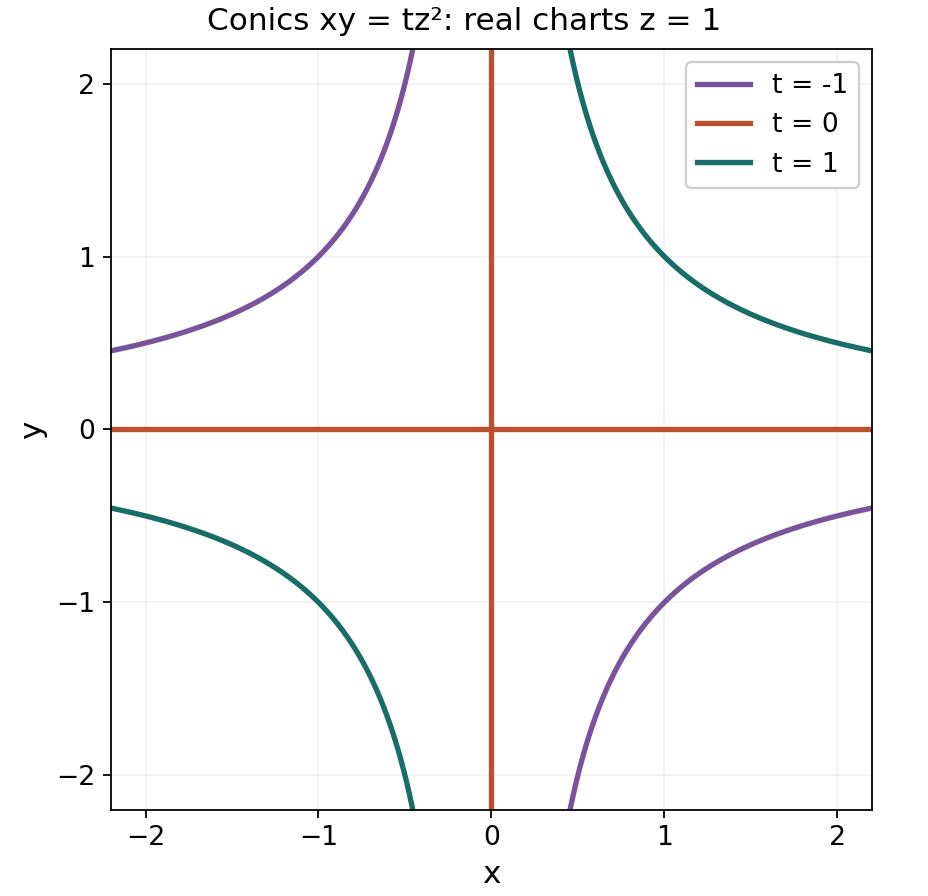
\includegraphics[width=0.95\linewidth,keepaspectratio]{../figures/conic-degeneration.png}}
\caption{Real affine charts of the conic family at t=-1, 0, and 1}
\end{figure}

\emph{Figure 1. The real charts z=1 of xy=tz², in the window
\(-2.2\le x,y\le2.2\). The red fiber t=0 consists of the two coordinate
axes. Points at infinity are omitted; this drawing shows the real
support, while the equations and flatness proof specify the scheme.
Every projective fiber has Hilbert polynomial 2n+1.}

\subsection{6. Exercises with
solutions}\label{exercises-with-solutions-6}

\textbf{Exercise 6.1 (easy: plane curves).} Compute the polynomial and
arithmetic genus of a plane curve of degree \(e\), and decide whether a
plane cubic can be a flat limit of twisted cubics as a reduced subscheme
of \(\mathbf P^3\).

\textbf{Solution.} The hypersurface sequence gives \(P(n)=en-e(e-3)/2\)
and \(p_a=(e-1)(e-2)/2\). A plane cubic has \(3n\), whereas a twisted
cubic has \(3n+1\). Theorem 4.2 excludes a flat family with precisely
these two fibers. It leaves open a limit whose underlying curve is a
plane cubic and whose structure sheaf has an additional length-one
contribution; Exercise 6.5 constructs it.

\textbf{Exercise 6.2 (easy: polynomial additivity).} Given
\(0\to F'\to F\to F''\to0\) on a proper scheme with a fixed invertible
\(L\), prove additivity of \(\chi\) and of \(P_{F,L}\). Does support
dimension itself add?

\textbf{Solution.} The finite long cohomology sequence proves Euler
additivity. Tensoring by each \(L^n\) preserves exactness, so the three
polynomial values satisfy additivity at every integer; polynomial
uniqueness gives \(P_F=P_{F'}+P_{F''}\). Supports satisfy
\(\operatorname{Supp}F=\operatorname{Supp}F'\cup\operatorname{Supp}F''\),
so their dimensions take the maximum, rather than the sum. For ample
\(L\), positivity of leading coefficients makes this maximum consistent
with the polynomial degree.

\textbf{Exercise 6.3 (medium: cubic and skew lines).} Compute the
Hilbert polynomials of a twisted cubic and of two skew lines directly
from their parametrizations and components.

\textbf{Solution.} The complete degree-three linear system on
\(\mathbf P^1\) gives \([s:u]\mapsto[s^3:s^2u:su^2:u^3]\). On the first
chart the ratios are \(1,a,a^2,a^3\), and on the last they are
\(b^3,b^2,b,1\); these recover the two affine charts of \(\mathbf P^1\).
The pulled-back twist is \(\mathcal O(3)\), so projective-line
cohomology gives \(\chi(\mathcal O(3n))=3n+1\) for every integer \(n\).
Skew lines are disjoint and their function sheaf is the direct sum of
the two component pushforwards, each with polynomial \(n+1\). Their sum
is \(2n+2\).

\textbf{Exercise 6.4 (medium: conic fibers).} Verify flatness and the
fiber polynomial for \(xy=tz^2\), including \(t=0\).

\textbf{Solution.} The monic relation gives the free standard-monomial
basis of Section 5, proving flatness on the projective charts. Its
degree-\(n\) basis, for \(n\geq0\), consists of \(x^az^{n-a}\),
\(0\leq a\leq n\), and \(y^bz^{n-b}\), \(1\leq b\leq n\). It has
\(2n+1\) elements independently of \(t\). The hypersurface Euler
calculation agrees with this eventual Hilbert function. At \(t=0\), the
two lines meet at one point, so their Euler polynomials add as
\((n+1)+(n+1)-1=2n+1\).

\textbf{Exercise 6.5 (hard: the embedded point in a cubic limit).} In
\(k[t,X,Y,Z,W]\), all four projective variables having degree one and
\(t\) degree zero, put \[
\begin{aligned}
g_1&=XW-tY^2,&g_2&=YW+tX^2-tYZ,\\
g_3&=W^2-tWZ+t^2XY,&g_4&=X^3+Y^3-XYZ.
\end{aligned}
\] Show that the projective family defined by these equations is flat,
its nonzero fibers are twisted cubics, and its zero fiber has a nodal
plane cubic and a length-one embedded point.

\textbf{Solution.} Use lexicographic order \(W>X>Y>Z\), treating
\(k[t]\) as the coefficient ring. The leading monomials are
\(XW,YW,W^2,X^3\), all with coefficient one. These polynomials form a
monic Gröbner basis over this ring. The pairs with relatively prime
leading monomials reduce to zero by the product criterion; the four
remaining pairs reduce by the first four identities below, in which each
right-hand product has leading monomial strictly below the corresponding
common multiple: \[
\begin{aligned}
Yg_1-Xg_2&=-t g_4,\\
Wg_1-Xg_3&=-tYg_2+tZg_1,\\
Wg_2-Yg_3&=tXg_1,\\
X^2g_1-Wg_4&=-Y^2g_2+YZg_1,\\
X^3g_3-W^2g_4&=(XYZ-Y^3)g_3-tWZg_4+t^2XYg_4.
\end{aligned}
\] The last pair also has relatively prime leading monomials, but its
displayed reduction checks it explicitly. The only other pair,
\(g_2,g_4\), is relatively prime. To justify the basis criterion, choose
an expression of an ideal element with smallest possible maximal leading
monomial. If leading terms cancel, the corresponding pair identity
replaces that cancellation by terms with smaller leading monomials;
pairs with relatively prime leading monomials have the elementary
product reduction. Thus a nonzero ideal element has leading monomial
divisible by one of the four displayed leading monomials. Division then
gives existence and uniqueness of a remainder outside that monomial
ideal. Monic division therefore makes the monomials outside
\((XW,YW,W^2,X^3)\) a free \(k[t]\)-basis of the quotient. This proves
flatness of the homogeneous algebra and hence of its projective charts,
by localization and degree-zero summands.

For \(t=a\ne0\), set \(U=Z-W/a\), \(V=X\), \(T=Y\), \(Q=W/a\). The first
three relations become the standard twisted-cubic relations \[
V^2-UT=0,\quad T^2-VQ=0,\quad VT-UQ=0.
\] The fourth follows from them, since \[
V(V^2-UT)+T(T^2-VQ)=V^3+T^3-VT(U+Q). 
\] The charts \(U\ne0\) and \(Q\ne0\) cover their projective scheme: if
both vanish at a homogeneous prime, the equations force \(V,T\) to
vanish too. The first chart has coordinate ring \(k[V/U]\), where
\(T/U=(V/U)^2\), \(Q/U=(V/U)^3\); the other chart gives the reciprocal
parameter. Thus the scheme is the cubic Veronese \(\mathbf P^1\). In the
original coordinates the parametrization is \[
[s:u]\longmapsto[s^2u:su^2:s^3+u^3:a u^3].
\]

At \(t=0\), the ideal is \[
(XW,YW,W^2,X^3+Y^3-XYZ).
\] The reduced curve lies in \(W=0\) and has equation \(F=X^3+Y^3-XYZ\).
This cubic is integral: in \(k[X,Y][Z]\) it is primitive and linear in
\(Z\), with relatively prime coefficients \(-XY\) and \(X^3+Y^3\), and
hence is irreducible. At \(P=[0:0:1:0]\), its affine equation is
\(x^3+y^3-xy\), with two distinct tangent lines \(x=0\) and \(y=0\). Its
derivatives show there is no other singular point, in every
characteristic. It is therefore a nodal plane cubic.

Let \(B_0\) be the special homogeneous ring. Killing \(W\) gives the
curve ring \(k[X,Y,Z]/(F)\). The kernel \((W)\) has basis \(WZ^j\),
\(j\geq0\), and as a graded module is \(k[Z](-1)\), annihilated by
\(X,Y,W\). After sheafification it is a length-one skyscraper at \(P\),
giving \[
0\to k(P)\to\mathcal O_{\operatorname{Proj}B_0}\to\mathcal O_C\to0.
\] It is embedded rather than an isolated point: its prime \((X,Y,W)\)
is the annihilator of the nonzero element \(W\), and properly contains
the curve's minimal prime \((W,F)\). The special polynomial is therefore
\(3n+1\). Counting standard monomials confirms this: for \(n\geq1\),
those without \(W\) contribute \(3n\), and \(WZ^{n-1}\) contributes one.
The embedded structure records exactly the constant term that a reduced
plane cubic would lose.

\textbf{Exercise 6.6 (challenging: jumping groups, constant sum).} On
\(\mathbf P^1_{k[t]}\), take the extension of \(\mathcal O\) by
\(\mathcal O(-2)\) whose class in \(H^1(\mathcal O(-2))=k[t]\) is \(t\).
Compute the cohomology of each fiber, and compare its Euler polynomial.

\textbf{Solution.} The usual Čech extension construction gives a vector
bundle \(E\); its exact sequence has locally free quotient and kernel,
so it is locally split as a sequence of sheaves and flat over the base.
On the fiber \(t=a\), the connecting homomorphism
\(H^0(\mathcal O)\to H^1(\mathcal O(-2))\) is multiplication by \(a\),
by the torsor/extension cocycle description. The long exact sequence
shows \(h^0(E_a)=h^1(E_a)=0\) if \(a\ne0\), and both are one if \(a=0\).
Their alternating sum is always zero. For all integer twists, additivity
gives \(P_{E_a}(n)=(n+1)+(n-1)=2n\), independent of \(a\). The
polynomial preserves an alternating sum, not each summand separately.

\subsection{References and further
direction}\label{references-and-further-direction}

\begin{itemize}
\tightlist
\item
  \textbf{{[}Stacks{]}} The Stacks project authors, \emph{The Stacks
  project}, in its AI Integrated Stacks Project edition: Euler
  additivity
  \href{https://kokunoyumeto.github.io/stacks-zh-hans-cn/en/varieties.html\#varieties-lemma-euler-characteristic-additive}{Tag
  08AA}; extension of fields
  \href{https://kokunoyumeto.github.io/stacks-zh-hans-cn/en/varieties.html\#varieties-lemma-euler-characteristic-extend-base-field}{Tag
  08AB}; proper pushforward
  \href{https://kokunoyumeto.github.io/stacks-zh-hans-cn/en/varieties.html\#varieties-lemma-euler-characteristic-morphism}{Tag
  0BEK}; polynomial twisting
  \href{https://kokunoyumeto.github.io/stacks-zh-hans-cn/en/varieties.html\#varieties-lemma-numerical-polynomial-from-euler}{Tag
  0BEM}; generic multiplicities
  \href{https://kokunoyumeto.github.io/stacks-zh-hans-cn/en/varieties.html\#varieties-lemma-numerical-polynomial-leading-term}{Tag
  0BEN}; eventual global sections
  \href{https://kokunoyumeto.github.io/stacks-zh-hans-cn/en/varieties.html\#varieties-lemma-hilbert-polynomial-H0}{Tag
  08AE}.
\item
  The degree assertion, with the zero sheaf separated, is also
  \href{https://kokunoyumeto.github.io/stacks-zh-hans-cn/en/varieties.html\#varieties-lemma-hilbert-polynomial-degree-support}{AI
  Integrated Stacks Project, varieties.tex,
  lemma-hilbert-polynomial-degree-support}. Section 3 proves it here,
  and proves the ample version on proper schemes. Dimension
  prerequisites:
  \href{https://kokunoyumeto.github.io/stacks-zh-hans-cn/en/algebra.html\#algebra-lemma-dimension-spell-it-out}{Tag
  00OS} and
  \href{https://kokunoyumeto.github.io/stacks-zh-hans-cn/en/algebra.html\#algebra-lemma-one-equation}{Tag
  00KW}.
\item
  The open reference treatments retain GNU FDL 1.2; this lesson's
  exposition and proofs are independently written CC0. The next lesson
  constructs the finite Grothendieck complex needed to control arbitrary
  fiber cohomology; the present flat-family proof already supplies its
  high-twist special case.
\end{itemize}

\section{Base change and the Grothendieck
complex}\label{base-change-and-the-grothendieck-complex}

\emph{Written by GPT-6.1 Sol (OpenAI), in Codex, at Ultra effort,
October 2026. Self-checked by the writing AI, GPT-6.1 Sol, at Ultra
effort. Public domain (CC0).}

Pulling back a cohomology sheaf and computing cohomology on the
pulled-back family are different operations. Flat change of the base
makes them agree. For a proper family with a flat coherent sheaf, a
stronger statement is available: one finite projective complex computes
cohomology after every change of the base. Its differentials, rather
than the ranks of its cohomology modules, retain the information needed
at exceptional fibers.

We use \href{affine-cohomology-and-serres-criterion.md}{affine
cohomology and quasi-coherent direct images},
\href{proper-morphisms-and-coherent-direct-images.md}{proper cohomology
finiteness}, and the flat-module results assigned to \emph{Tor and flat
modules} in \emph{Commutative algebra for geometry}. For the initial
derived construction we use
\href{../derived-categories-and-sheaf-operations/flat-modules-and-k-flat-resolutions.html}{K-flat
resolutions},
\href{../derived-categories-and-sheaf-operations/derived-tensor-products-and-tor-sheaves.html}{derived
tensor} and the
\href{../derived-categories-and-sheaf-operations/derived-pullback-and-pushforward.html}{pullback--pushforward
adjunction}. The earlier programme proof of adjunction is \emph{Derived
pullback and pushforward}, Theorem 2.2; Proposition 3.1 proves
composition, and Theorem 1.1 constructs derived pullback. These supply
the units, counits and composition used in Section 1. Our finite
projective replacement and its universal tensor comparison are proved in
Section 3.

\subsection{1. Constructing the
comparison}\label{constructing-the-comparison}

Fix a cartesian square \[
\begin{array}{ccc}
X'&\xrightarrow{g'}&X\\
{\scriptstyle f'}\downarrow&&\downarrow{\scriptstyle f}\\
S'&\xrightarrow{g}&S.
\end{array}
\] Let \(F\) be quasi-coherent on \(X\), and put \(F'=g'^*F\). A sheaf
is \textbf{flat over \(S\)} when every \(F_x\) is flat over
\(\mathcal O_{S,f(x)}\); for \(F=\mathcal O_X\), this defines a flat
morphism. Base change preserves this stalkwise condition. Flatness of
\(F\) and flatness of \(g\) will enter different theorems.

The canonical comparison maps are \[
\beta^q:g^*R^qf_*F\longrightarrow R^qf'_*F'.
\] Here is a derived construction that also applies to a nonflat \(g\).
Derived adjunction turns the composite \[
Lf'^*Lg^*Rf_*F
\cong Lg'^*Lf^*Rf_*F
\longrightarrow Lg'^*F
\longrightarrow g'^*F
\] into a map \(Lg^*Rf_*F\to Rf'_*F'\). The first arrow is the
pullback--pushforward counit; the last is the natural map from derived
pullback of a sheaf to its degree-zero, ordinary pullback. Commutation
of the two derived pullbacks follows from equality of the composite
morphisms and composition of derived pullback. It does not assert that
derived pullback is exact.

There is a natural cohomology edge map \[
g^*H^q(C)\longrightarrow H^q(Lg^*C)
\] for a bounded-above cohomology object \(C\). Locally, choose a
bounded-above free resolution \(P\) of its complex over \(A\), and use
the cocycle map \[
H^q(P)\otimes_A B\longrightarrow H^q(P\otimes_A B).
\] A cocycle tensored with an element of \(B\) is still a cocycle; an
original boundary becomes a boundary. Right exactness of tensor lets
this descend from the cocycle module to \(H^q(P)\otimes B\). Homotopic
comparison maps of free resolutions induce the same map, so the edge is
intrinsic and compatible with restriction. Composing it with the
cohomology map of the derived comparison defines \(\beta^q\). For the
quasi-compact, quasi-separated morphisms used below, the boundedness
needed here is the affine-cover bound from the third lesson. For flat
\(g\), the edge is simply the identification \(g^*H^q(C)=H^q(g^*C)\).

The construction is functorial in \(F\) and in successive base changes:
units, counits and pullback composition give the same map for a
composite square as for the two successive squares. On affine charts
with a Čech model, it is the cocycle comparison just described. Thus the
isomorphisms proved below concern these canonical maps, not a separately
chosen identification of abstract vector spaces.

\textbf{Proposition 1.1 (affine morphisms).} If \(f\) is affine, every
\(\beta^q\) is an isomorphism for every base change \(g\), without a
flatness assumption.

\textbf{Proof.} Higher direct images of a quasi-coherent sheaf under an
affine morphism are zero, and the same holds for \(f'\). Locally write
\(S=\operatorname{Spec}A\), \(X=\operatorname{Spec}R\),
\(S'=\operatorname{Spec}B\), and \(F=\widetilde M\). The pullback sheaf
corresponds to \[
M\otimes_R(R\otimes_A B)\cong M\otimes_A B.
\] This is precisely the degree-zero base-change map. The tensor
identity proves the assertion in degree zero, and the vanishing proves
it in higher degrees. \(\square\)

The hypothesis concerns the morphism \(f\). Affineness of \(g\) alone
does not guarantee comparison isomorphisms; a closed point of an affine
parameter scheme is already a nonflat affine base change.

\subsection{2. Flat base change, including nonseparated
schemes}\label{flat-base-change-including-nonseparated-schemes}

\textbf{Theorem 2.1 (flat base change).} If \(f\) is quasi-compact and
quasi-separated, \(F\) is quasi-coherent, and \(g\) is flat, then \[
g^*R^qf_*F\xrightarrow{\sim}R^qf'_*F'\quad(q\geq0).
\] In particular, for a flat ring map \(A\to B\) and a quasi-compact,
quasi-separated \(A\)-scheme, \[
H^q(X,F)\otimes_A B\xrightarrow{\sim}H^q(X_B,F_B).
\]

\textbf{Proof.} First suppose \(S,S'\) are affine and \(X\) is
separated. Choose a finite affine cover \(U_1,\ldots,U_r\). Its
intersections are affine, so the finite ordered complex \(C^\bullet\) of
their section modules computes cohomology. The induced cover after base
change again has affine intersections. Proposition 1.1 identifies its
section complex with \(C^\bullet\otimes_A B\). Flatness of \(B\)
preserves kernels and images and gives \[
H^q(C^\bullet)\otimes_A B\cong H^q(C^\bullet\otimes_A B).
\] The identification is the canonical cocycle map.

For a quasi-separated \(X\), a finite affine cover still exists, but its
intersections need not be affine. Each intersection \(U_I\) is
quasi-compact and separated: it is an open subscheme of one of the
affine \(U_i\). The case just proved therefore applies to every \(U_I\).
Use the Čech-to-cohomology spectral sequence of the second lesson, in
the form \[
E_1^{p,q}=\bigoplus_{|I|=p+1}H^q(U_I,F)\Longrightarrow H^{p+q}(X,F).
\] Tensoring this spectral sequence with flat \(B\) preserves its
successive kernels, images and cohomology. The comparison with the
base-changed cover is an isomorphism on every first-page term, by the
separated case. Hence it is an isomorphism on every page and on the
filtered abutments. The cover has finitely many intersections and each
has a finite affine-cover cohomological bound, so there are only
finitely many possibly nonzero terms. Convergence and comparison
therefore involve finite filtrations and prove the asserted global
identity.

Finally work locally on \(S'\), with its affine open contained over an
affine open of \(S\). The higher direct images are quasi-coherent by the
third lesson, and over this affine base they are the sheaves associated
to the cohomology modules just compared. The global identities give the
sheaf comparison locally, and canonical functoriality glues them.
\(\square\)

Notice that \(F\) need not be flat over the original base in this
theorem. Tensor is exact because the \emph{change of base} is flat. In
contrast, we next keep \(F\) flat and permit every change of base.

\subsection{3. A finite projective
replacement}\label{a-finite-projective-replacement}

We first prove the algebraic step, retaining its tensor behavior rather
than only its cohomology over the original ring.

\textbf{Lemma 3.1 (bounded flat complexes).} Let \(A\) be Noetherian.
Let \(C^\bullet\) be a complex of flat \(A\)-modules, zero outside
\([a,b]\), with finite cohomology modules. There is a complex
\(K^\bullet\) of finite projective modules, also zero outside \([a,b]\),
and a quasi-isomorphism \[
K^\bullet\longrightarrow C^\bullet
\] that remains a quasi-isomorphism after tensoring with every
\(A\)-module.

\textbf{Proof.} We construct a bounded-above finite free resolution of
the complex, then truncate its unnecessary left tail.

Start with no terms of \(P\), and attach them in descending degrees,
beginning at \(b\). Suppose terms \(P^{j+1},\ldots,P^b\) and a chain map
\(f:P\to C\) have been constructed, with its cone \(D\) having zero
cohomology in degrees above \(j\). The cone terms and differential are
\[
D^i=C^i\oplus P^{i+1},\qquad d_D(c,p)=(d_Cc+f(p),-d_Pp).
\] Its cohomology modules are finite. This holds initially for \(C\),
and remains true for a cone of a map from a finite complex of finite
free modules: its long exact sequence expresses cohomology as extensions
of subquotients of finite modules, which are finite because \(A\) is
Noetherian.

Choose finitely many cocycles \((c_\ell,p_\ell)\) generating \(H^j(D)\).
Set \(P^j\) equal to the finite free module on these choices and define
\[
f(e_\ell)=c_\ell,\qquad d_P(e_\ell)=-p_\ell.
\] The cocycle equations give \(d_P^2=0\) and \(d_Cf=fd_P\). In the new
cone, the differential of \((0,e_\ell)\) is \((c_\ell,p_\ell)\), so
\(H^j\) is killed while higher cohomology remains zero. Finiteness of
lower cohomology is preserved by the same long exact sequence.
Continuing indefinitely to the left gives a chain map \(P\to C\), with
each \(P^j\) finite free and \(P^j=0\) for \(j>b\). Its cone is acyclic:
in any fixed degree, the construction kills the cohomology after
finitely many stages, and later stages do not change it. Thus \(P\to C\)
is a quasi-isomorphism.

We need a tensor fact about its cone. An acyclic bounded-above complex
\(T\) of flat modules remains acyclic after every tensor product. At its
last nonzero degree, the preceding differential surjects onto the last
term. The kernel is flat, because a kernel between flat middle and flat
quotient modules is flat. Repeating downward shows all cycle modules are
flat and every sequence \[
0\to Z^i(T)\to T^i\to Z^{i+1}(T)\to0
\] remains exact under tensor. These tensor sequences imply acyclicity
after tensoring. The downward induction reaches any specified degree in
finitely many steps even if the complex is unbounded to the left.
Applying it to the cone of \(P\to C\) gives \[
H^i(P\otimes_A M)\cong H^i(C\otimes_A M)=0\quad(i<a)
\] for every \(M\).

Now put \(Q=\operatorname{coker}(P^{a-1}\to P^a)\). It is finite, and
the exact sequence \[
\cdots\to P^{a-2}\to P^{a-1}\to P^a\to Q\to0
\] is a free resolution of \(Q\). Exactness uses \(H^i(P)=0\) for
\(i<a\). Therefore \[
\operatorname{Tor}_1^A(Q,M)=H^{a-1}(P\otimes_A M)=0
\] for all \(M\), since the differential through degree \(a\) is the
same in that resolution. Thus \(Q\) is flat. It is finitely presented
over Noetherian \(A\), so it is finite projective by the flat-module
criterion.

Define \(K^a=Q\), \(K^i=P^i\) for \(a<i\leq b\), and all other terms
zero. The map \(P^a\to C^a\) kills the preceding image because
\(C^{a-1}=0\); it factors through \(Q\), giving a chain map \(K\to C\).
Truncation preserves all cohomology, so this map is a quasi-isomorphism.
Its cone is a bounded acyclic complex of flat modules. The tensor fact
proves that \(K\otimes M\to C\otimes M\) is a quasi-isomorphism for
every \(M\), as required. \(\square\)

The finite replacement does not come from assuming Čech terms are
finite, nor from assuming the ring has finite global dimension.
Finiteness of the \emph{cohomology} constructs the finite free
approximation. Flatness and its bounded range then make the last
retained quotient projective.

\textbf{Theorem 3.2 (the Grothendieck complex).} Let \(A\) be
Noetherian, \(f:X\to\operatorname{Spec}A\) proper, and \(F\) coherent
and flat over \(A\). There is a bounded complex \(K\) of finite
projective \(A\)-modules, in nonnegative degrees, such that for every
\(A\)-algebra \(B\), \[
H^q(K\otimes_A B)\cong H^q(X_B,F_B),
\] functorially in \(B\). More generally
\(H^q(K\otimes_A M)\cong H^q(X,F\otimes_A M)\) for every \(A\)-module
\(M\).

\textbf{Proof.} Properness makes \(X\) quasi-compact and separated. Take
a finite affine cover with \(r\) members. Its ordered Čech complex
\(C\), zero outside \([0,r-1]\), computes \(F\)-cohomology. Every term
is \(A\)-flat: for any injection of \(A\)-modules, tensoring the sheaf
preserves injectivity at all stalks, and taking sections on an affine
intersection preserves exactness of quasi-coherent sheaves. This is the
section-module flatness argument already used for high twists in the
preceding lesson. Its cohomology is finite by proper finiteness. Apply
Lemma 3.1 to obtain \(K\to C\).

Every affine intersection stays affine after a base change. Its section
module for \(F_B\) is the original one tensored with \(B\), so the
complex after base change is \(C\otimes_A B\). It computes
\(H^q(X_B,F_B)\). The universal tensor quasi-isomorphism of Lemma 3.1
identifies its cohomology with that of \(K\otimes_A B\). For an
arbitrary module \(M\), the same affine correspondence identifies
\(C\otimes_A M\) with the Čech complex of \(F\otimes_A M\). All maps
arise from a fixed chain map and affine tensor identifications, so are
compatible with homomorphisms of modules and algebras. \(\square\)

In derived language, a bounded complex of finite projective modules
represents a \textbf{perfect} object. Thus the theorem proves that
\(R\Gamma(X,F)\) is perfect and \[
R\Gamma(X,F)\otimes_A^L B\cong R\Gamma(X_B,F_B)
\] for every \(B\). This is stronger than flat base change. It does not
imply that \(H^q(X,F)\otimes B\to H^q(X_B,F_B)\) is always an
isomorphism: taking cohomology of a tensor product is still distinct
from tensoring its cohomology. The finite complex makes that distinction
computable.

\subsection{4. Euler constancy and explicit
models}\label{euler-constancy-and-explicit-models}

\textbf{Corollary 4.1.} Under Theorem 3.2, the fiber Euler
characteristic \(s\mapsto\chi(X_s,F_s)\) is locally constant on
\(\operatorname{Spec}A\).

\textbf{Proof.} The complex \(K\otimes_A\kappa(s)\) is a finite complex
of finite-dimensional vector spaces computing fiber cohomology. Image
cancellation gives \[
\chi(X_s,F_s)=\sum_i(-1)^i\dim_{\kappa(s)}(K^i\otimes_A\kappa(s))
=\sum_i(-1)^i\operatorname{rank}_s K^i.
\] Each finite projective module has locally constant rank. There are
finitely many of them, so their alternating sum is locally constant.
\(\square\)

For \(\mathcal O\) on \(\mathbf P^1_A\), use \(K=A[0]\). The
projective-space computation gives \(H^0=B\) and all higher cohomology
zero for every \(A\)-algebra \(B\). More generally \(\mathcal O(d)\) has
the explicit free complex concentrated in degree zero for \(d\geq0\), in
degree one for \(d\leq-2\), and the zero complex for \(d=-1\). This
includes \(\mathcal O(-2)\) represented by \(A\) in degree one.

For the family of conics \(xy=tz^2\) over \(A=k[t]\), the monic
homogeneous equation makes the family flat, as proved in the preceding
lesson. Over every \(A\)-algebra \(B\), multiplication by the equation
remains injective in the polynomial ring: its leading coefficient is
one. The sequence on \(\mathbf P^2_B\) \[
0\to\mathcal O(-2)\to\mathcal O\to\mathcal O_{\mathcal C_B}\to0
\] and projective-space cohomology give a Grothendieck complex \(A[0]\)
for the structure sheaf. Twisting once replaces \(\mathcal O(-2)\) by
\(\mathcal O(-1)\) and \(\mathcal O\) by \(\mathcal O(1)\), giving
\(A^3[0]\) for \(\mathcal O_{\mathcal C}(1)\). These computations work
on the reducible special fiber as well.

A more revealing example is the rank-two extension on
\(\mathbf P^1_{k[t]}\) \[
0\to\mathcal O(-2)\to E\to\mathcal O\to0
\] with extension class \(t\). The projective-line calculations and its
connecting map give the model \[
K=[\,A\xrightarrow{t}A\,]\quad\text{in degrees }0,1.
\] Indeed the cohomology triangle for the extension is the fiber of
multiplication by \(t\) between the two copies of \(A\), which is this
two-term complex; choosing the generator of \(H^1(\mathcal O(-2))\)
fixes that sign. Tensoring with any \(B\) replaces the differential by
multiplication by the image of \(t\). Over the original integral ring,
\(H^0(E)=0\) and \(H^1(E)=A/(t)\). At the zero fiber the differential is
zero and both fiber groups are \(k\). Thus \(\beta^0\) is the map
\(0\to k\), while \(\beta^1\) is an isomorphism. The Euler
characteristic is zero everywhere. Retaining the differential recovers
the missing fiber sections.

\subsection{5. Exercises with
solutions}\label{exercises-with-solutions-7}

\textbf{Exercise 5.1 (easy: affine comparison).} For an affine morphism
and an arbitrary change of base, write the degree-zero comparison
explicitly and explain the higher-degree statement.

\textbf{Solution.} With \(A\to R\), \(A\to B\), and \(M\) an
\(R\)-module, the map is \(M\otimes_A B\to M\otimes_R(R\otimes_A B)\),
taking \(m\otimes b\) to \(m\otimes(1\otimes b)\). The inverse takes
\(m\otimes(r\otimes b)\) to \(rm\otimes b\). Higher source and target
sheaves are zero by affine vanishing. Neither flatness of \(M\) nor
flatness of \(B\) is needed.

\textbf{Exercise 5.2 (easy: flat Čech terms).} Prove flatness over \(A\)
of the section modules on affine intersections when \(F\) is flat over
\(A\). Identify where separatedness is used in Theorem 3.2.

\textbf{Solution.} Every stalk \(F_x\) is flat over its parameter local
ring and therefore over \(A\), since localization of \(A\) is flat.
Tensoring an injection of \(A\)-modules with \(F\) is thus stalkwise
injective. The resulting sheaves are quasi-coherent, and their sections
on an affine open form an exact sequence. Hence tensoring the affine
section module preserves injections, proving flatness. Separatedness
ensures that the finite cover's intersections are affine; without it,
the single section complex need not compute higher cohomology.

\textbf{Exercise 5.3 (medium: the alternating ranks).} Derive Euler
constancy from a Grothendieck complex, and decide whether it forces its
cohomology ranks to be locally constant.

\textbf{Solution.} On each fiber, boundaries cancel in the alternating
dimension sum, leaving the alternating ranks of the finitely many
projective terms. Those ranks are locally constant, which proves Euler
constancy. Cohomology ranks need not be: for \([A\xrightarrow{t}A]\),
both are zero away from \(t=0\) and both are one there. The alternating
difference stays zero.

\textbf{Exercise 5.4 (medium: the conic hyperplane bundle).} Compute a
Grothendieck complex for \(\mathcal O(1)\) on \(xy=tz^2\), and check its
behavior under the nonflat base change \(k[t]\to k[t]/(t^2)\).

\textbf{Solution.} The twisted hypersurface sequence is
\(0\to\mathcal O(-1)\to\mathcal O(1)\to\mathcal O_{\mathcal C}(1)\to0\).
On \(\mathbf P^2_B\), \(\mathcal O(-1)\) has no cohomology and
\(\mathcal O(1)\) has only \(H^0=B^3\), for every \(B\). The monic
equation preserves injectivity even when \(B\) has nilpotents. Thus
\(K=A^3[0]\) works, and over \(B=A/(t^2)\) it gives \(B^3\) in degree
zero and zero otherwise. This is a genuine arbitrary-base-change
calculation, not an application of the flat-base-change theorem.

\textbf{Exercise 5.5 (hard: truncate a free approximation).} For a
bounded flat complex with finite cohomology over a Noetherian ring,
explain why a finite free approximation may have an infinite left tail,
and prove that its truncation term at the original lower bound is
projective.

\textbf{Solution.} Successively killing the cone's top cohomology
constructs finite free terms, but new kernel classes can appear one
degree lower at each step. The ring need not have finite global
dimension, so this process need not stop. Let the original flat complex
start in degree \(a\), and let \(P\) be the resulting bounded-above free
approximation. Its acyclic flat cone remains acyclic after tensoring, by
the cycle induction of Lemma 3.1. Thus \(H^{a-1}(P\otimes M)=0\) for
every \(M\). The free tail through \(P^a\) resolves
\(Q=\operatorname{coker}(P^{a-1}\to P^a)\), so this equality is
\(\operatorname{Tor}_1(Q,M)=0\). It implies flatness of \(Q\); finite
generation and Noetherianness give finite presentation, hence
projectivity. Replacing the whole left tail by \(Q\) retains the
cohomology and universal tensor comparison. This is the complete
truncation mechanism, not a finite global-dimension argument.

\textbf{Exercise 5.6 (challenging: why the flat-sheaf hypothesis
matters).} Take the proper identity map
\(X=\operatorname{Spec}k[t]\to\operatorname{Spec}k[t]\) and
\(F=\widetilde{k[t]/(t)}\). Show that no bounded finite projective
complex can compute its ordinary fiber cohomology for all base changes
in the manner of Theorem 3.2, although \(R\Gamma(X,F)\) itself is
perfect.

\textbf{Solution.} Its fiber is zero away from \(t=0\), and at zero it
is \(k\), with no positive cohomology because the fibers are affine. A
hypothetical complex would therefore have fiber Euler characteristic
zero generically and one at zero. Its alternating term ranks would be
locally constant, contradicting connectedness of
\(\operatorname{Spec}k[t]\). Meanwhile \(k[t]/(t)\) has the finite free
resolution \([A\xrightarrow{t}A]\) in degrees \(-1,0\), so it is
perfect. Tensoring that resolution with \(k\) creates a nonzero
degree-\(-1\) Tor group. Derived base change remembers this group;
ordinary pullback of \(F\) does not. Thus perfectness alone does not
remove the need for flatness in the universal ordinary-family
comparison.

\subsection{References and the next use of the
complex}\label{references-and-the-next-use-of-the-complex}

\begin{itemize}
\tightlist
\item
  \textbf{{[}Stacks{]}} The Stacks project authors, \emph{The Stacks
  project}, in its AI Integrated Stacks Project edition: affine
  comparison
  \href{https://kokunoyumeto.github.io/stacks-zh-hans-cn/en/coherent.html\#coherent-lemma-affine-base-change}{Tag
  02KG}; flat comparison
  \href{https://kokunoyumeto.github.io/stacks-zh-hans-cn/en/coherent.html\#coherent-lemma-flat-base-change-cohomology}{Tag
  02KH}; base-change Čech complexes
  \href{https://kokunoyumeto.github.io/stacks-zh-hans-cn/en/coherent.html\#coherent-lemma-base-change-complex}{Tag
  01XM}; proper flat perfect direct images
  \href{https://kokunoyumeto.github.io/stacks-zh-hans-cn/en/coherent.html\#coherent-lemma-perfect-direct-image}{Tag
  07VK}. The construction and finite replacement needed here are proved
  in Sections 2--3.
\item
  The exact earlier programme foundation is
  \href{../derived-categories-and-sheaf-operations/derived-pullback-and-pushforward.html}{\emph{Derived
  pullback and pushforward}, Theorems 1.1 and 2.2 and Proposition 3.1},
  proving pullback, adjunction and composition. The corresponding
  supplementary open adjunction is
  \href{https://kokunoyumeto.github.io/stacks-zh-hans-cn/en/cohomology.html\#cohomology-lemma-adjoint}{Tag
  079W}, using
  \href{https://kokunoyumeto.github.io/stacks-zh-hans-cn/en/derived.html\#derived-lemma-derived-adjoint-functors}{derived
  adjoint functors} and its
  \href{https://kokunoyumeto.github.io/stacks-zh-hans-cn/en/derived.html\#derived-lemma-pre-derived-adjoint-functors-general}{general
  localization proof}. Composition of derived pullbacks is
  \href{https://kokunoyumeto.github.io/stacks-zh-hans-cn/en/cohomology.html\#cohomology-lemma-derived-pullback-composition}{cohomology,
  lemma-derived-pullback-composition}.
\item
  These open reference texts retain GNU FDL 1.2. This exposition, its
  finite replacement proof and exercise solutions are independently
  written CC0. The next lesson studies ranks of the differentials to
  prove semicontinuity and the precise criterion for a cohomology
  base-change map to be an isomorphism.
\end{itemize}

\section{Semicontinuity and Grauert's
theorem}\label{semicontinuity-and-grauerts-theorem}

\emph{Written by GPT-6.1 Sol (OpenAI), in Codex, at Ultra effort,
October 2026. Self-checked by the writing AI, GPT-6.1 Sol, at Ultra
effort. Public domain (CC0).}

The dimensions of fiber cohomology can increase at special parameters. A
finite complex explains both this increase and the stronger conditions
that prevent it. Matrix ranks control semicontinuity; lifting fiber
classes controls the comparison map; and a reduced base turns pointwise
vanishing of matrix entries into actual vanishing.

We use \href{base-change-and-the-grothendieck-complex.md}{Base change
and the Grothendieck complex}. First take a proper morphism \(f:X\to S\)
with \(S\) Noetherian and \(F\) coherent and flat over \(S\). All
conclusions also apply to a proper morphism of finite presentation over
an arbitrary scheme, with \(F\) finitely presented and flat over \(S\).
The following argument proves the finite complex in this full setting.

\textbf{Lemma 0.1 (a finite complex over an arbitrary base).} If \(A\)
is any ring, \(X\to\operatorname{Spec}A\) is proper of finite
presentation and \(F\) is finitely presented and \(A\)-flat, there is a
finite projective complex \(K\), in nonnegative degrees, which computes
\(H^q(X_B,F_B)\) after every \(A\)-algebra change \(B\).

\textbf{Proof.} Write \(A=\operatorname{colim}A_i\), where the \(A_i\)
are its finite-type \(\mathbf Z\)-subalgebras and hence Noetherian. The
earlier \href{../AG-MO/AG-MO-03.html}{\emph{Limits and Noetherian
approximation}, Theorems 4.1--4.2 and 5.1} descends a finitely presented
scheme and its separated diagonal to a separated finite-type
\(X_i/A_i\). The sheaf also descends: choose finitely many affine
charts, finite presentation matrices on them, and gluing maps on finite
affine refinements of overlaps. Matrices, their inverses and the cocycle
identities involve finitely many coefficients and finitely many
equalities, which hold at a sufficiently late stage. This gives finitely
presented \(F_i\) with pullback \(F\).

We justify descent of properness rather than assuming it. Apply the
Noetherian Chow theorem of the earlier \emph{Projective morphisms and
Chow's lemma}, Theorem 4.1, to \(X_i/A_i\). It gives a proper surjection
\(Y_i\to X_i\) with \(Y_i\) quasi-projective over \(A_i\), thus immersed
in a finite projective space. After change to \(A\),
\(Y\to X\to\operatorname{Spec}A\) is proper. Its immersion into
projective space is consequently closed by the graph argument of the
Serre lesson. Eventual closed-immersion descent in \emph{Limits},
Theorem 4.2, makes \(Y_j\) projective over \(A_j\) at a later stage. The
proper surjection \(Y_j\to X_j\) then makes \(X_j\) universally closed:
after any base change, the image in the base of a closed subset
\(C\subset X_j\) equals the image of its closed inverse image in
\(Y_j\), which is closed by properness. Together with separatedness and
finite type, this proves \(X_j/A_j\) proper.

Flatness also descends with these hypotheses. The earlier
\href{../AG-FSE/AG-FSE-02.html\#6-finite-presentations-over-an-arbitrary-base}{\emph{Flatness
criteria}, Lemma 6.2} proves that flatness at a point of a finitely
presented limit module holds at its contracted point at some Noetherian
stage. Theorem 5.2 there proves that this is an open condition at that
stage. Pull back these flat opens to \(X\). They cover \(X\), which is
quasi-compact, so finitely many suffice. Pass to a common stage and take
their union there. Subsequent pullbacks of these opens remain flat by
ordinary flat base change. The closed complement has empty inverse
limit; the finite-cover descent of \emph{Limits}, Lemma 2.1, makes that
complement empty at a sufficiently late stage. Hence the entire \(F_j\)
is \(A_j\)-flat. This explains exactly how pointwise eventual flatness
yields one global stage.

Now \(X_j\) is proper over Noetherian \(A_j\), and \(F_j\) is coherent
and \(A_j\)-flat. The Grothendieck-complex construction in the preceding
lesson gives a finite projective nonnegative \(K_j\) and its universal
comparison to the finite affine-cover complex. Pull back to \(A\) and
put \(K=K_j\otimes_{A_j}A\). The cover and every section module pull
back termwise, by the affine module/sheaf equivalence; its intersections
are affine by separatedness. For every \(A\)-algebra \(B\), the
universal comparison for \(K_j\otimes B\) is therefore the comparison to
the cover of \(X_B,F_B\). It computes the required cohomology and is
canonical at the level of the derived comparison maps. Finite
projectivity and the nonnegative degree range survive tensoring.
\(\square\)

Locally on an affine base, therefore, such a \(K\) computes all fiber
and base-changed cohomology in either setting.

We denote the canonical fiber comparison by \[
\varphi^q(s):(R^qf_*F)\otimes\kappa(s)\longrightarrow H^q(X_s,F_s).
\] On an affine neighborhood it is the cocycle map
\(H^q(K)\otimes\kappa(s)\to H^q(K\otimes\kappa(s))\). Comparing these
two expressions for cohomology is the purpose of this lesson.

\subsection{1. Semicontinuity from
minors}\label{semicontinuity-from-minors}

After restricting to an affine open where every projective term is free,
write \(r_q=\operatorname{rank}K^q\). Let \(d^q\) be its differential
and \(\rho_q(s)\) the rank of the matrix over \(\kappa(s)\). Since
\(d^qd^{q-1}=0\), linear algebra gives \[
h^q(s):=\dim_{\kappa(s)}H^q(X_s,F_s)
=r_q-\rho_{q-1}(s)-\rho_q(s).
\] The rank of a matrix is lower semicontinuous: the locus of rank at
least \(r\) is the union of the principal opens where some \(r\times r\)
minor is invertible. The sum of the two ranks is the rank of their block
diagonal matrix, so it too is lower semicontinuous.

\textbf{Theorem 1.1 (semicontinuity).} Under the stated proper
flat-sheaf hypotheses, every \(h^q:S\to\mathbf Z_{\geq0}\) is upper
semicontinuous. Its level sets are locally constructible, and its values
commute with arbitrary base change of parameter schemes.

\textbf{Proof.} On each trivializing affine, the displayed formula makes
\(\{h^q\geq n\}\) the locus where the block diagonal matrix has rank at
most \(r_q-n\). This is closed, defined by the minors of size
\(r_q-n+1\), with the usual empty or whole-locus conventions at the
extreme bounds. The closed-locus assertion is local, so holds on \(S\).
Each equality locus \(\{h^q=n\}\) is the difference of the closed loci
\(\{h^q\geq n\}\) and \(\{h^q\geq n+1\}\), hence locally constructible.
For a parameter \(s'\) above \(s\), the new geometric cohomology complex
is the old fiber complex tensored with \(\kappa(s')\). Extending a field
preserves its ranks and cohomology dimensions, proving the final
assertion. \(\square\)

Upper semicontinuity allows an increase on a closed locus. It does not
say that every special fiber acquires new cohomology or that individual
cohomology modules over the parameter ring are locally free. Those
require further information about the matrices.

\subsection{2. Remove the invertible
blocks}\label{remove-the-invertible-blocks}

\textbf{Lemma 2.1 (a minimal complex near a point).} For a fixed \(s\),
after restricting to an affine neighborhood and trivializing the terms,
the complex can be replaced by a finite free complex whose differentials
are all zero over \(\kappa(s)\). The replacement preserves its
cohomology after every base change.

\textbf{Proof.} If a differential matrix has an entry invertible at
\(s\), shrink so that it is a unit and use elementary row and column
operations to make it the sole nonzero entry in its row and column,
equal to one. The relation between consecutive differentials forces the
incoming differential's component in the corresponding source summand to
be zero, and the outgoing differential's component from the
corresponding target summand to be zero. Thus the two copies of \(A\),
with identity between them, split off as a direct summand complex in
consecutive degrees. This summand is contractible, including after every
tensor product. Remove it. Each removal reduces the sum of the term
ranks by two, so after finitely many removals no entry is invertible at
\(s\). All remaining entries lie in the maximal ideal of
\(\mathcal O_{S,s}\), which means the residue-field differentials are
zero. All operations and splittings occurred on a neighborhood of \(s\),
proving the lemma. \(\square\)

Here minimality refers to the chosen point. Other points of the
neighborhood may still have nonzero residue-field differentials. At the
chosen point, \[
H^q(K\otimes\kappa(s))=K^q\otimes\kappa(s).
\] Surjectivity of a cohomology comparison now says that a basis of this
space lifts to actual cocycles.

\textbf{Lemma 2.2 (lifting cocycles kills a differential).} For a
complex as in Lemma 2.1, \(\varphi^q(s)\) is surjective if and only if
\(d^q=0\) in the local ring at \(s\). If it is surjective, \(d^q\) is
zero on a smaller neighborhood.

\textbf{Proof.} If the map is surjective, choose finitely many actual
cocycles in \(K^q\) whose reductions give a basis of
\(K^q\otimes\kappa(s)\). The square matrix having these cocycles as
columns has determinant invertible in the local ring, so they form a
basis of \(K^q\) there. The differential kills every basis vector, hence
is zero. Its finitely many entries vanish in the localization and
consequently on some smaller neighborhood. Conversely, if \(d^q=0\)
locally, every element of \(K^q\) is a cocycle. Its reduction maps onto
the fiber cohomology because the incoming differential reduces to zero
by minimality. Thus \(\varphi^q(s)\) is surjective. \(\square\)

This proof does not need finite generation of the entire cocycle module
over an arbitrary base. Surjectivity selects finitely many cocycles, and
an invertible determinant already makes them a basis of the finite free
term.

\subsection{3. Cohomology and base
change}\label{cohomology-and-base-change}

\textbf{Theorem 3.1 (the surjectivity criterion).} Suppose
\(\varphi^q(s)\) is surjective. There is an open neighborhood \(U\) of
\(s\) on which formation of \(R^qf_*F\) commutes with every base change.
In particular the comparison is an isomorphism at every point of \(U\).
Under this hypothesis, the following are equivalent:

\begin{enumerate}
\def\labelenumi{\arabic{enumi}.}
\tightlist
\item
  \(\varphi^{q-1}(s)\) is surjective;
\item
  \(R^qf_*F\) is locally free on a neighborhood of \(s\).
\end{enumerate}

For \(q=0\), set all negative direct images and fiber cohomology to
zero; the first condition is automatic.

\textbf{Proof.} Apply Lemmas 2.1--2.2 and shrink so that \(d^q=0\). Then
\[
H^q(K)=\operatorname{coker}(d^{q-1}:K^{q-1}\to K^q).
\] Tensor is right exact, so for every \(A\)-algebra \(B\) on this
neighborhood, \[
H^q(K)\otimes_A B
\cong\operatorname{coker}(d^{q-1}\otimes B)
=H^q(K\otimes_A B).
\] This is exactly the canonical comparison. The identity localizes and
glues for arbitrary scheme base changes, proving the first part.

If \(\varphi^{q-1}(s)\) is surjective, Lemma 2.2 kills \(d^{q-1}\) after
a further shrinking. Now \(H^q(K)=K^q\), so it is finite free there.

Conversely assume \(H^q(K)\) is free over the local ring \(A_s\). The
sequence \[
0\to N:=\operatorname{im}d^{q-1}\to K^q\to H^q(K)\to0
\] splits, since its quotient is free. Thus \(N\) is a finite direct
summand of \(K^q\). Minimality gives \(N\subset\mathfrak m_sK^q\), so
its inclusion is zero after tensoring with the residue field. But a
split inclusion remains injective after tensoring. Hence
\(N/\mathfrak m_sN=0\), and Nakayama gives \(N=0\). Therefore
\(d^{q-1}=0\) locally and Lemma 2.2 proves surjectivity of
\(\varphi^{q-1}(s)\). In degree zero the nonnegative model already has
\(K^{-1}=0\), giving the stated convention. \(\square\)

The hypothesis refers to the comparison map, not merely to equality of
dimensions of two spaces. Once it holds, right exactness of a cokernel
supplies arbitrary base change in that degree. Local freeness adds a
condition on the preceding differential. These are two distinct
conclusions of the theorem.

\subsection{4. Grauert's theorem and the reduced
base}\label{grauerts-theorem-and-the-reduced-base}

\textbf{Theorem 4.1 (Grauert).} Suppose \(S\) is reduced and \(h^q\) is
locally constant. Then \(R^qf_*F\) is finite locally free and its
formation commutes with every base change.

\textbf{Proof.} Fix \(s\) and choose a minimal complex near it. Let
\(r=\operatorname{rank}K^q\). The two residue-field differentials at
\(s\) vanish, so \(h^q(s)=r\). Restrict to a neighborhood where \(h^q\)
is this constant. For every point \(u\) there, \[
r=h^q(u)=r-\rho_{q-1}(u)-\rho_q(u).
\] Both ranks are nonnegative, hence both are zero at every point. Every
matrix entry of \(d^{q-1}\) and \(d^q\) therefore belongs to every prime
of the affine coordinate ring. Such entries lie in its nilradical.
Reducedness makes that nilradical zero, so both differentials actually
vanish. Consequently \(H^q(K)=K^q\), and the same is true after every
tensor product. This gives finite local freeness and comparison with
every base change on a neighborhood of \(s\); these assertions glue on
\(S\). \(\square\)

Reducedness is doing precise work: residue fields detect whether an
entry is nilpotent, but do not detect whether that nilpotent entry is
zero. Over \(A=k[\epsilon]/(\epsilon^2)\), the complex \[
[\,A\xrightarrow{\epsilon}A\,]\quad\text{in degrees }0,1
\] has fiber dimensions one in each degree on the one-point base. Yet
its cohomology modules are \((\epsilon)\) and \(A/(\epsilon)\), neither
free over \(A\), and its degree-zero comparison is zero. This complex is
realized by the flat rank-two extension of \(\mathcal O\) by
\(\mathcal O(-2)\) on \(\mathbf P^1_A\) with class \(\epsilon\). Thus
the failure occurs for a proper flat family with a vector bundle, not
only for an unrelated algebraic complex.

\subsection{5. Vanishing and the structure
sheaf}\label{vanishing-and-the-structure-sheaf}

\textbf{Corollary 5.1 (vanishing gives local freeness).} If
\(R^qf_*F=0\) for every \(q>0\), then \(f_*F\) is finite locally free
and commutes with arbitrary base change. Its higher direct images also
vanish after every base change.

\textbf{Proof.} On an affine neighborhood, use the nonnegative finite
projective complex \(K\). It is exact in positive degrees. Begin at the
last term: the preceding differential surjects onto a projective module,
so splits. Its kernel is a finite projective direct summand of the
preceding term. Exactness in the next degree gives another surjection
onto this kernel, which again splits. Continue down to degree zero. It
follows that \(K\) is the direct sum of contractible projective pairs
and its finite projective \(H^0\) in degree zero. All these splittings
survive every tensor product. The universal comparison of the
Grothendieck complex proves the assertions. \(\square\)

\textbf{Theorem 5.2 (constants in a proper flat family).} Let \(f\) be
proper, flat and of finite presentation, with nonempty geometrically
reduced and geometrically connected fibers. Then the unit is an
isomorphism \[
\mathcal O_S\xrightarrow{\sim}f_*\mathcal O_X,
\] and remains an isomorphism after every base change. No reducedness
assumption on \(S\) is required.

\textbf{Proof.} By the global-functions calculation in the proper-image
lesson, a nonempty geometrically reduced and geometrically connected
proper scheme over a field has that field as its constants. Thus
\(H^0(X_s,\mathcal O_{X_s})=\kappa(s)\). The unit section is an actual
global section and maps to \(1\) in this fiber space. Therefore
\(\varphi^0(s)\) is surjective at every point. Theorem 3.1 applies in
degree zero, where the preceding comparison is automatically surjective:
\(f_*\mathcal O_X\) is finite locally free, with arbitrary base change.
Its fibers all have dimension one. The unit map between these rank-one
locally free sheaves is an isomorphism on every residue field; its
coefficient is consequently a unit in every local ring, so it is an
isomorphism. Its universal comparison identifies the base-changed unit
with the same isomorphism over every \(S'\). \(\square\)

The nonempty convention is stated explicitly; the Stacks convention for
geometrically connected schemes already includes it {[}Tag 0362{]}. Over
an imperfect field, geometric reducedness is essential in the constants
assertion. The purely inseparable field example in the proper-image
lesson shows why ordinary reducedness is insufficient. Universality here
includes nilpotent base changes, which would not follow from checking
only reduced parameter schemes.

\textbf{Corollary 5.3 (vanishing on every fiber).} In either setting at
the start of the lesson, assume \(H^q(X_s,F_s)=0\) for every point \(s\)
and every \(q>0\). Then \(f_*F\) is finite locally free and commutes
with every base change, and all positive higher direct images vanish
universally. No reducedness assumption on \(S\) is required.

\textbf{Proof.} Fix \(s\) and use the nonnegative finite projective
complex which computes every base change. Lemma 2.1 cancels its unit
differential entries and gives a finite free complex minimal at \(s\),
after shrinking the affine neighborhood. Every differential of its
residue-field complex is zero. Thus its degree-\(q\) term has
residue-field dimension \(h^q(s)\). For every \(q>0\) this is zero, so
the corresponding free term has rank zero and is the zero module. There
are finitely many terms, and the complex on this neighborhood is
therefore concentrated in degree zero. It is finite free there, with the
same property after tensoring with any algebra. Universal comparison
identifies its degree-zero cohomology with \(f_*F\) and gives vanishing
in all positive degrees. These neighborhoods cover \(S\), and the
canonical base-change maps glue the conclusions. \(\square\)

\subsection{6. A line bundle with jumping
sections}\label{a-line-bundle-with-jumping-sections}

Let \(E\) be a smooth projective geometrically connected genus-one curve
over an algebraically closed field \(k\), and fix \(p\in E(k)\). On
\(E\times E\), let \(\Delta\) be the diagonal and consider \[
\mathcal L=\mathcal O_{E\times E}(\{p\}\times E-\Delta).
\] Both divisors are Cartier. For the second projection its fiber at
\(q\) is \(L_q=\mathcal O_E(p-q)\), and \(\mathcal L\) is flat over the
base: it is invertible on a scheme flat over \(E\).

Here is the needed curve calculation without importing later duality or
a nonaffine Zariski Main factorization. Suppose a second independent
section of \(\mathcal O_E(p)\) exists. Dividing by its canonical section
gives a nonconstant rational function \(f\) with its only pole a simple
pole at the rational point \(p\). At every closed point the smooth
curve's local ring is a discrete valuation ring, as proved in the
earlier \emph{Discrete valuation rings, normal rings and Serre's
criterion}. Using \(f\) or \(1/f\), according to its valuation, defines
a morphism \(h:E\to\mathbf P^1\). It is proper by its graph.

We first prove its function field is \(k(f)\). A function \(g\) regular
on \(E\setminus\{p\}\) has at most a pole of some order \(m\) at \(p\).
The leading coefficient of its Laurent expansion there belongs to \(k\),
since \(p\) is rational. Subtract a suitable scalar multiple of \(f^m\)
to reduce that pole order. Induction leaves a global regular function on
\(E\), which is in \(k\) by the constants calculation of the
proper-coherence lesson. Thus every such \(g\) belongs to \(k[f]\). For
an arbitrary rational function \(u\), its poles away from \(p\) form a
finite set: the complement of a nonempty regularity open on a Noetherian
integral curve is finite. For each such point \(q\), the residue
\(f(q)\) is algebraic over \(k\); a nonzero polynomial \(P_q\in k[T]\)
vanishes at it. Consequently \(P_q(f)\) has positive valuation at \(q\).
Multiplying \(u\) by sufficiently high powers of these finitely many
polynomials removes every pole away from \(p\). The product is in
\(k[f]\) by the preceding argument. Hence \(u\in k(f)\), proving
\(k(E)=k(f)\).

For a closed \(y\in\mathbf P^1\) and any point \(q\) above it, both
local rings are discrete valuation subrings of this same field. Their
inclusion is local. If \(\pi\) is a uniformizer of
\(\mathcal O_{\mathbf P^1,y}\), its valuation in \(\mathcal O_{E,q}\) is
positive, while every unit of the first ring remains a unit. An element
of negative first valuation would therefore have negative second
valuation and could not belong to \(\mathcal O_{E,q}\). This proves
equality of the two local rings. There cannot be two points above \(y\):
the resulting two morphisms from the spectrum of this valuation ring to
the separated curve agree on its dense generic point, and their closed
equalizer is the whole integral spectrum. Properness makes the image of
\(h\) closed; nonconstancy makes it contain the generic point, so it is
surjective. It is now bijective and closed, hence a homeomorphism, and
all its local ring maps, including the generic one, are isomorphisms. It
is therefore an isomorphism of schemes. This contradicts
\(h^1(\mathcal O_E)=1\), since the projective-line calculation gives
zero. Thus \(h^0(\mathcal O_E(p))=1\). In
\(0\to\mathcal O_E\to\mathcal O_E(p)\to k(p)\to0\), the first two
section spaces are the constants. Its boundary
\(k\to H^1(\mathcal O_E)=k\) is an isomorphism, proving
\(H^1(\mathcal O_E(p))=0\). The argument persists after every field
extension.

An invertible sheaf of degree zero with a nonzero section is trivial:
its section has an effective zero divisor of degree zero, hence no
zeros, so trivializes the sheaf. If \(L_q\) is trivial,
\(\mathcal O_E(p)\cong\mathcal O_E(q)\). Each has its canonical section
vanishing at its indicated point. Their section space is
one-dimensional, so the isomorphism identifies these sections up to
scalar; their zero divisors coincide and \(p=q\). Conversely \(L_p\) is
trivial. This argument is preserved after extension of the ground field,
so also applies at the generic parameter. Therefore \[
h^0(E,L_q)=\begin{cases}1&q=p,\\0&q\ne p.\end{cases}
\] The Euler characteristic is zero for all \(q\): adding the point
\(p\) and subtracting the point \(q\) in the two divisor sequences
cancel their length-one Euler contributions. Since the curve has
cohomological dimension one, \(h^1(E,L_q)=h^0(E,L_q)\). Both jump at the
closed point \(p\), consistently with semicontinuity and Euler
constancy.

This family also illustrates the hypothesis in Theorem 3.1. Its
degree-zero direct image is zero. Indeed it is torsion-free on the
integral base, because multiplication by a nonzero base function is
injective on the flat sheaf at every stalk, and taking sections
preserves this injection; it has zero generic rank, and it is finite by
proper coherence, so it is zero. Thus at \(p\) the comparison is
\(0\to k\), which is not surjective. The exceptional fiber section
cannot be lifted from a neighborhood.

\subsection{7. Exercises with
solutions}\label{exercises-with-solutions-8}

\textbf{Exercise 7.1 (easy: minors).} Prove upper semicontinuity of the
middle cohomology dimension of a three-term complex of finite free
modules, and write its jump locus as a determinantal locus.

\textbf{Solution.} For ranks \(a,b,c\) and differential ranks
\(r_1,r_2\), the dimension is \(b-r_1-r_2\). The sum is the rank of the
block diagonal matrix formed by the two differentials. Thus dimension at
least \(n\) is defined by all minors of size \(b-n+1\) of that matrix.
This is closed. Subtracting the next such closed locus gives a locally
closed equality locus.

\textbf{Exercise 7.2 (medium: the genus-one family).} Compute \(h^0\),
\(h^1\), and the degree-zero comparison at the special point of the
family \(\mathcal O_E(p-q)\).

\textbf{Solution.} A nonzero section of a degree-zero bundle trivializes
it. The one-dimensional section space of \(\mathcal O(p)\), established
in Section 6, shows triviality occurs exactly when \(q=p\). Thus both
dimensions are one there and zero elsewhere, since their Euler
difference is zero. The flat sheaf gives torsion-free direct-image
sections on the integral base, and generic vanishing makes that direct
image zero. Its comparison at \(p\) is therefore \(0\to k\), not a
surjection. This identifies the precise missing hypothesis of the
base-change criterion.

\textbf{Exercise 7.3 (medium: geometrically integral fibers).} Deduce
universal \(f_*\mathcal O_X=\mathcal O_S\) for a proper flat finitely
presented morphism with geometrically integral fibers. Explain whether
the base must be reduced.

\textbf{Solution.} Geometrically integral fibers are nonempty,
geometrically reduced and geometrically connected. Theorem 5.2 applies
directly and proves the universal equality. The base may have
nilpotents. In its proof the unit provides a lift of the fiber's
constant section, so degree-zero comparison is surjective without using
reducedness or Grauert's theorem.

\textbf{Exercise 7.4 (hard: Grauert from a minimal model).} Starting
with a finite free complex minimal at \(s\), prove the reduced-base
theorem and identify the exact step that fails on a nonreduced base.

\textbf{Solution.} Minimality makes the fiber dimension in degree \(q\)
equal to the rank of the corresponding term. If this dimension is
constant nearby, both adjacent differential ranks must be zero at every
point. Their entries vanish in every residue field, hence lie in the
nilradical. A reduced coordinate ring has zero nilradical, so both
matrices vanish and the cohomology is the free middle term, before and
after every tensor product. Without reducedness this only proves that
the entries are nilpotent. Multiplication by a nonzero nilpotent need
not be a zero differential, so its kernels and cokernels need not be
free.

\textbf{Exercise 7.5 (hard: a nonreduced counterexample).} Use the
extension with class \(\epsilon\) over \(k[\epsilon]/(\epsilon^2)\) to
verify failure of Grauert's conclusion despite constant fiber
dimensions.

\textbf{Solution.} The extension is a vector bundle on
\(\mathbf P^1_A\), so is flat over \(A\). Its cohomology model is
\([A\xrightarrow{\epsilon}A]\) in degrees zero and one. The sole fiber
has zero differential, with both dimensions one. Over \(A\), the kernel
is \((\epsilon)\) and the cokernel is \(k\); both have length one, while
a nonzero finite free \(A\)-module has length a positive even integer.
Hence neither is free. In degree zero the cocycle \(\epsilon\) reduces
to zero, so the comparison \((\epsilon)\otimes_A k\to k\) is the zero
map. This verifies the geometric counterexample completely.

\textbf{Exercise 7.6 (challenging: the adjacent comparison).} For
\(K=[A\xrightarrow{t}A]\) in degrees zero and one over \(A=k[t]\), check
both parts of Theorem 3.1 at \(t=0\), taking \(q=1\).

\textbf{Solution.} The outgoing degree-one differential is zero, so
\(H^1(K)=A/(t)\), and its comparison with \(H^1(K\otimes B)=B/tB\) is an
isomorphism for every \(B\). In particular \(\varphi^1(0)\) is
surjective. The degree-zero comparison is \(0\to k\), since
multiplication by \(t\) is injective over \(A\) and becomes zero on that
fiber. It is not surjective, consistently with \(A/(t)\) not being
locally free near zero. The first comparison criterion gives universal
base change in degree one, while the second correctly rejects local
freeness there.

\subsection{References and hypotheses}\label{references-and-hypotheses}

\begin{itemize}
\tightlist
\item
  \textbf{{[}Stacks{]}} The Stacks project authors, \emph{The Stacks
  project}, in its AI Integrated Stacks Project edition. The
  finite-presentation extension of the Grothendieck complex is
  \href{https://kokunoyumeto.github.io/stacks-zh-hans-cn/en/perfect.html\#perfect-lemma-flat-proper-perfect-direct-image-general}{Tag
  0B91}; its full Noetherian-approximation proof is
  \href{https://kokunoyumeto.github.io/stacks-zh-hans-cn/en/perfect.html\#perfect-lemma-base-change-tensor-perfect}{Tag
  0A1H}. Semicontinuity is
  \href{https://kokunoyumeto.github.io/stacks-zh-hans-cn/en/perfect.html\#perfect-lemma-jump-loci}{Tag
  0BDI}; vanishing and local freeness
  \href{https://kokunoyumeto.github.io/stacks-zh-hans-cn/en/perfect.html\#perfect-lemma-vanishing-implies-locally-free}{Tag
  0D4E}; universal constants
  \href{https://kokunoyumeto.github.io/stacks-zh-hans-cn/en/perfect.html\#perfect-lemma-proper-flat-geom-red-connected}{Tag
  0E0L}. Sections 1--5 provide the matrix proofs and both parts of the
  surjectivity theorem used here.
\item
  Section 6 proves the genus-one curve input directly using the earlier
  discrete-valuation and constants facts;
  \href{https://kokunoyumeto.github.io/stacks-zh-hans-cn/en/curves.html\#curves-lemma-degree-more-than-2g-2}{Tag
  0E3B} is supplementary curve-duality reading. The nonempty convention
  for geometric connectedness is
  \href{https://kokunoyumeto.github.io/stacks-zh-hans-cn/en/varieties.html\#varieties-definition-geometrically-connected}{Tag
  0362}. These are explicit routine inputs; the reduced-base Grauert
  theorem and comparison criterion have complete proofs in this lesson.
\item
  The open reference treatments retain GNU FDL 1.2. This exposition,
  proofs, examples and solutions are independently written CC0.
  Reducedness is required for the pointwise-rank argument in Grauert's
  theorem; it is not required for the surjectivity criterion or the
  universal constants theorem.
\end{itemize}

\section{The theorem on formal
functions}\label{the-theorem-on-formal-functions}

\emph{Written by GPT-6.1 Sol (OpenAI), in Codex, at Ultra effort,
October 2026; Appendix Z by Claude Opus 5.5 (Anthropic), October 2026.
Self-checked by the writing AI. Original text: public domain (CC0). See
the \href{licensing.html}{course notice} for authorship.}

A fiber remembers a family at one parameter. Its successive
infinitesimal neighborhoods remember powers of that parameter's maximal
ideal. Formal functions identifies the inverse limit of their cohomology
with the completion of a finite cohomology module. The individual
comparison maps can fail to be isomorphisms; what makes the theorem work
is a uniform bound on how long their errors persist.

We use \href{proper-morphisms-and-coherent-direct-images.md}{proper
coherent direct images},
\href{affine-cohomology-and-serres-criterion.md}{affine cohomology and
Serre's criterion}, and
\href{base-change-and-the-grothendieck-complex.md}{flat base change}.
\href{../AG-CA/AG-CA-19.html\#3-noetherian-exactness-tensoring-and-flatness}{Completion,
Theorems 3.1--3.3} supplies exact completion of finite modules over
Noetherian rings and faithful flatness when the completion ideal lies in
the Jacobson radical, including maximal-ideal completion of a Noetherian
local ring. The dimension consequences in Section 5 use
\href{../ag-etale-cohomology/cohomological-dimension-and-the-kunneth-formula.html\#7-the-bound-for-all-finite-type-schemes}{Cohomological
dimension and the Künneth formula, Lemma 7.1}, the full Noetherian
topological vanishing proof for arbitrary abelian sheaves. No flatness
assumption on the coherent sheaf is imposed in this lesson.

\subsection{0. A normality input in the algebraic Zariski Main
proof}\label{a-normality-input-in-the-algebraic-zariski-main-proof}

The quasi-finite input used in Section 5 has an algebraic Zariski Main
proof whose supporting coefficient argument requires polynomial
normality over an arbitrary normal domain. A proof for polynomial rings
over fields alone would not suffice. We supply the general statement
here. The valuation existence input is the written
\href{../AG-GS/prerequisites/AG-MO/valuation-rings-and-separatedness.html}{Valuation
rings and separatedness, Theorem 2.1}; it gives a valuation ring in a
specified field dominating a specified local subring, without a
Noetherian hypothesis or a discrete-value assumption.

\textbf{Lemma 0.1 (polynomial normality).} If \(R\) is an integrally
closed domain, then \(R[x_1,\ldots,x_n]\) is an integrally closed domain
for every finite \(n\).

\textbf{Proof.} Put \(F=\operatorname{Frac}R\). First we prove that
\(R\) is the intersection of all valuation subrings of \(F\) containing
\(R\). If \(z\in F\setminus R\), then \(z\) is not integral over \(R\).
In the ring \(R[z^{-1}]\), the element \(z^{-1}\) is not a unit: an
equation \[
1=z^{-1}(a_0+a_1z^{-1}+\cdots+a_mz^{-m})
\] would yield a monic polynomial equation for \(z\) over \(R\), after
multiplication by \(z^{m+1}\). Choose a maximal ideal containing
\(z^{-1}\) and localize at it. The earlier valuation theorem gives a
valuation ring \(V\subset F\) dominating this local ring. Thus
\(R\subset V\), while \(z^{-1}\) is in its maximal ideal and
\(z\notin V\). This separates every \(z\notin R\) from the intersection
and proves the assertion.

For such a valuation ring, let \(v:F^*\to\Gamma\) be its ordered value
group, with \(V=\{0\}\cup\{a:v(a)\geq0\}\). This group can be
constructed as \(F^*/V^*\), ordered by divisibility in \(V\). For a
nonzero polynomial \(h=\sum a_ix^i\in F[x]\), define \[
w(h)=\min_i v(a_i),
\] ignoring zero coefficients. We have \(w(hg)=w(h)+w(g)\): divide each
polynomial by a coefficient of least value. The resulting polynomials
have coefficients in \(V\) and nonzero reductions in
\((V/\mathfrak m_V)[x]\); their product has nonzero reduction because
this polynomial ring over a field is a domain. Also
\(w(h+g)\geq\min(w(h),w(g))\), with equality when the two values differ.
Consequently a sum with a unique term of strictly least value cannot
vanish.

Let \(u\in F(x)\) be integral over \(R[x]\). It is integral over
\(F[x]\), so \(u\in F[x]\). To justify this last assertion directly,
write \(u=a/b\) with coprime polynomials in the Euclidean domain
\(F[x]\). A monic integral equation implies that \(b\) divides \(a^m\).
Bézout's identity for \(a,b\) forces \(b\) to be a unit. Thus \(u\) is a
polynomial.

For every valuation ring \(V\) above, write its integral equation as \[
u^m+c_1(x)u^{m-1}+\cdots+c_m(x)=0,
\qquad c_i(x)\in R[x]\subset V[x].
\] If \(w(u)<0\), the term \(u^m\) has value \(m w(u)\), strictly less
than the value of every other nonzero term, since \(w(c_i)\geq0\). This
contradicts the least-value property. Hence every coefficient of \(u\)
belongs to \(V\). The intersection assertion puts all coefficients in
\(R\), proving that \(R[x]\) is integrally closed. Induction on the
number of variables proves the lemma. \(\square\)

This proof supplies the polynomial-normality step of the supporting
algebraic argument. Not all of the other inputs of that argument are
proved here.

\subsection{1. The completion map}\label{the-completion-map}

Let \(A\) be Noetherian, \(I\subset A\) an ideal,
\(f:X\to\operatorname{Spec}A\) proper, and \(F\) coherent. For
\(n\geq1\), put \[
X_n=X\times_A\operatorname{Spec}(A/I^n),\qquad F_n=F|_{X_n}.
\] The closed immersion \(i_n:X_n\hookrightarrow X\) has
\(i_{n*}F_n=F/I^nF\). Since closed immersion pushforward is exact and
has no positive direct images, we may compute \[
H^q(X_n,F_n)=H^q(X,F/I^nF).
\] Set \(M^q=H^q(X,F)\), a finite \(A\)-module by proper finiteness. The
quotient map on sheaves induces \[
M^q/I^nM^q\longrightarrow H^q(X_n,F_n),
\] because \(I^n\) annihilates the target. These maps are compatible
with reduction from \(n+1\) to \(n\). We seek an isomorphism from \[
\widehat{M^q}=\varprojlim_n M^q/I^nM^q
\] to the inverse limit of the right-hand terms. Completion here is with
respect to \(I\); neither \(A\) nor \(M^q\) is assumed complete in
advance.

The theorem is not a claim that every finite-level map is an
isomorphism. For example, the extension bundle on \(\mathbf P^1_{k[t]}\)
with class \(t\) has \(H^0(X,E)=0\), but has a nonzero section on the
fiber \(t=0\). We will return to its infinitesimal neighborhoods in
Exercise 7.6.

\subsection{2. All powers at once}\label{all-powers-at-once}

The \textbf{Rees algebra} is \[
R=\bigoplus_{n\geq0}I^nT^n\subset A[T],\qquad R_0=A.
\] If \(I=(a_1,\ldots,a_r)\), then \(R\) is generated by the degree-one
elements \(a_iT\), hence is a quotient of a polynomial algebra in
finitely many variables over \(A\). It is Noetherian. The symbol \(T\)
records degree; it need not itself belong to \(R\).

\textbf{Lemma 2.1 (graded cohomological finiteness).} For each
\(q\geq0\), the graded module \[
Q^q=\bigoplus_{n\geq0}H^q(X,I^nF)T^n
\] is finite over \(R\).

\textbf{Proof.} Form \(X_R=X\times_A\operatorname{Spec}R\), with affine
projection \(\pi:X_R\to X\). On \(X\), the graded sheaf
\(\bigoplus I^nF\) is a module over \(\mathcal O_X\otimes_A R\): a
degree-\(d\) element acts by multiplication into the degree shifted by
\(d\). It is a quotient of \(F\otimes_A R\), by the degreewise maps
\(F\otimes_A I^n\to I^nF\). The affine module/sheaf correspondence gives
a coherent sheaf \(G\) on \(X_R\) with \[
\pi_*G=\bigoplus_{n\geq0}I^nF.
\] Coherence follows because \(X_R\) is Noetherian and this sheaf is
locally a finite module, generated by a finite set of degree-zero
generators of \(F\).

The map \(X_R\to\operatorname{Spec}R\) is proper by base change. Proper
cohomology finiteness makes \(H^q(X_R,G)\) finite over \(R\). Affine
pushforward and Leray identify it with \(H^q(X,\pi_*G)\). Finally
cohomology of quasi-coherent sheaves on the quasi-compact,
quasi-separated scheme \(X\) commutes with filtered colimits, by the
third lesson. A direct sum is the filtered colimit of finite partial
sums, so \[
H^q(X,\pi_*G)=\bigoplus_{n\geq0}H^q(X,I^nF).
\] The identifications preserve multiplication and grading. This is the
asserted finite graded module. \(\square\)

We next extract two consequences. Write \[
J_n^q=\operatorname{im}\bigl(H^q(X,I^nF)\to M^q\bigr),
\qquad K_n^q=\ker\bigl(H^q(X,I^nF)\to M^q\bigr).
\] Both collections respect graded multiplication. Indeed inclusion of
ideal powers commutes with multiplying a section or cohomology class by
an element of \(I^d\). Thus \(\bigoplus J_n^qT^n\) is a finite graded
image module of \(Q^q\), and \(\bigoplus K_n^qT^n\) is a finite graded
submodule, using Noetherianness of \(R\).

\textbf{Lemma 2.2 (bounds on the image and kernel).} There are integers
\(c_J,c_K\geq0\) such that \[
I^nM^q\subset J_n^q\subset I^{n-c_J}M^q\quad(n\geq c_J),
\] and the transition map \(K_m^q\to K_n^q\) is zero whenever
\(m\geq n+c_K\).

\textbf{Proof.} Multiplication by an element of \(I^n\) factors as
\(F\to I^nF\to F\), proving the first inclusion. Choose finitely many
homogeneous generators of the image module, all in degrees at most
\(c_J\). The degree-\(n\) part is a sum of \(I^{n-d}J_d^q\) over
generator degrees \(d\leq c_J\). Each is contained in \(I^{n-c_J}M^q\),
proving the second inclusion. This is the cohomological analogue of an
Artin--Rees bound.

Choose homogeneous kernel generators \(k_\ell\in K_{d_\ell}^q\) with
\(d_\ell\leq c_K\). An element of \(K_m^q\) is a sum of products
\(a_\ell k_\ell\), with \(a_\ell\in I^{m-d_\ell}\). If \(m\geq n+c_K\),
each such coefficient is a sum of products \(ba'\), where \(b\in I^n\)
and \(a'\in I^{m-d_\ell-n}\). Under transition to \(H^q(X,I^nF)\), its
product with \(k_\ell\) is computed by first including \(I^{d_\ell}F\)
into \(F\), then multiplying by \(a'\), then by \(b\) into \(I^nF\). The
initial inclusion sends \(k_\ell\) to zero, by definition of the kernel.
Hence every product maps to zero. This proves the uniform transition
bound. \(\square\)

A system whose sufficiently distant transition maps to each fixed term
are zero is called \textbf{pro-zero}. Its individual terms may be
nonzero; its inverse limit is zero because each coordinate of a
compatible family is the image of a distant, necessarily zero,
transition. Lemma 2.2 supplies this stronger, bounded form of
disappearance for the kernel system.

\subsection{3. Stabilization of the thickened
cohomology}\label{stabilization-of-the-thickened-cohomology}

The short exact sequence \(0\to I^nF\to F\to F/I^nF\to0\) gives the
exact sequence \[
0\to M^q/J_n^q\longrightarrow H^q(X_n,F_n)\longrightarrow K_n^{q+1}\to0.
\tag{1}
\] It is a sequence of inverse systems. The left transitions are
surjective because \(J_m^q\subset J_n^q\) for \(m\geq n\). The right
system is pro-zero by Lemma 2.2 in degree \(q+1\).

\textbf{Proposition 3.1 (the Mittag--Leffler bound).} For fixed \(q\),
choose \(c\) as the kernel bound in degree \(q+1\). Then for
\(m\geq n+c\), \[
\operatorname{im}\bigl(H^q(X_m,F_m)\to H^q(X_n,F_n)\bigr)
=\operatorname{im}\bigl(M^q\to H^q(X_n,F_n)\bigr).
\] Consequently the thickened-cohomology system is Mittag--Leffler.

\textbf{Proof.} In diagram (1) for indices \(m,n\), the right transition
is zero. Therefore the middle transition lands in the left submodule
\(M^q/J_n^q\). It contains all of that submodule: the left transition
\(M^q/J_m^q\to M^q/J_n^q\) is onto, and these left modules inject into
the respective middle terms. Thus its image is exactly the claimed
submodule. The image is independent of all sufficiently large \(m\),
which is the Mittag--Leffler condition. \(\square\)

We can now take the limit without an unexplained exchange of limits and
cohomology. If \((u_n)\) is a compatible family of middle classes in
(1), its images in \(K_n^{q+1}\) form a compatible family in a pro-zero
system, so are all zero. Thus each \(u_n\) lies in the injective left
term, with a unique preimage. These preimages are automatically
compatible. We obtain the canonical identification \[
\varprojlim_n H^q(X_n,F_n)=\varprojlim_n M^q/J_n^q.
\tag{2}
\] This also proves why a transient class on a small thickening need not
define a class in the inverse limit. Compatibility with every higher
thickening is a real constraint.

\subsection{4. Global and stalk forms of formal
functions}\label{global-and-stalk-forms-of-formal-functions}

\textbf{Theorem 4.1 (formal functions).} Under the hypotheses of Section
1, the canonical maps give an isomorphism \[
\widehat{H^q(X,F)}\xrightarrow{\sim}\varprojlim_n H^q(X_n,F_n).
\] It is an isomorphism of \(\widehat A\)-modules and a homeomorphism
for their inverse-limit topologies.

\textbf{Proof.} Combine (2) with the inclusions from Lemma 2.2: \[
I^nM^q\subset J_n^q,\qquad J_{n+c_J}^q\subset I^nM^q.
\] They say that the two descending filtrations \((I^nM^q)\) and
\((J_n^q)\) are cofinal. The identification (2) also preserves the limit
topologies: each left term is a discrete submodule of the corresponding
middle term, and its unique coordinate preimage is continuous on that
submodule. The first inclusions give the canonical continuous map
between the inverse limits of the corresponding quotients. The second
give its inverse by taking the cofinal shifted indices \(n+c_J\). The
two composites are the usual transitions and hence induce the identity
on limits. Both maps are continuous for the quotient limit topologies,
proving the homeomorphism. The maps arise from \(A\)-linear maps at all
levels, where \(I^n\) annihilates the cohomology of \(F_n\), and so
preserve the induced \(\widehat A\)-action. \(\square\)

\textbf{Corollary 4.2 (the stalk form).} Let \(f:X\to S\) be proper,
\(S\) locally Noetherian, \(F\) coherent, and \(s\in S\). Put
\(A_s=\mathcal O_{S,s}\), with maximal ideal \(\mathfrak m_s\), and \[
X_n=X\times_S\operatorname{Spec}(A_s/\mathfrak m_s^n),\qquad F_n=F|_{X_n}.
\] Then \[
\widehat{(R^qf_*F)_s}\cong\varprojlim_n H^q(X_n,F_n)
\] as \(\widehat{A_s}\)-modules.

\textbf{Proof.} The canonical map \(\operatorname{Spec}A_s\to S\) is
flat: on an affine neighborhood it is localization. Flat base change and
the affine description of quasi-coherent direct images identify the
stalk with
\(H^q(X\times_S\operatorname{Spec}A_s,F|_{X\times_S\operatorname{Spec}A_s})\).
The local ring is Noetherian, the changed morphism proper, and the
changed sheaf coherent. Apply Theorem 4.1 with ideal \(\mathfrak m_s\).
Its thickenings are precisely the displayed \(X_n\), since their
parameter maps factor through \(\operatorname{Spec}A_s\). \(\square\)

\subsection{5. Dimension and finiteness
consequences}\label{dimension-and-finiteness-consequences}

\textbf{Theorem 5.1 (vanishing above a fiber's dimension).} For the
morphism of Corollary 4.2, \[
(R^qf_*F)_s=0\quad\text{if }q>\dim X_s.
\]

\textbf{Proof.} Each \(X_n\) has the same underlying topological space
as \(X_s\): the extra ideal is nilpotent and therefore belongs to every
prime. That space is Noetherian, of finite dimension \(d\), because
\(X_s\) is of finite type over a field. The Noetherian topological
vanishing theorem,
\href{../ag-etale-cohomology/cohomological-dimension-and-the-kunneth-formula.html\#7-the-bound-for-all-finite-type-schemes}{Cohomological
dimension and the Künneth formula, Lemma 7.1}, gives \(H^q(X_n,F_n)=0\)
for \(q>d\). Formal functions makes the completed stalk zero. The
uncompleted stalk is finite by proper coherence. For a finite module
over a Noetherian local ring, completion preserves the residue-field
quotient; zero completion implies \(M/\mathfrak mM=0\), and Nakayama
implies \(M=0\). This proves the assertion. An empty fiber gives empty
thickenings and the same conclusion in every degree. \(\square\)

The vanishing is a statement about the whole stalk, stronger than a
statement about its tensor with the residue field. In particular, if all
fiber dimensions are at most \(d\), then \(R^qf_*F=0\) for \(q>d\),
without a flatness assumption.

\textbf{Theorem 5.2 (proper with finite fibers is finite).} A proper
morphism over a locally Noetherian base whose fibers have finitely many
points is finite.

\textbf{Proof.} Its fibers are finite type over fields. Such schemes
with finitely many points are zero-dimensional by Noether normalization.
Indeed an affine chart admits a finite integral surjection onto affine
space of its dimension; a positive-dimensional affine space over any
field has infinitely many points, so a finite-point chart cannot have
positive dimension. Their zero-dimensional coordinate rings are
finite-dimensional by Noether normalization. Thus Theorem 5.1 makes
\(R^1f_*G=0\) for every coherent \(G\).

Work over an affine Noetherian neighborhood \(S=\operatorname{Spec}A\).
Its inverse image \(X\) is Noetherian, separated and quasi-compact. Any
finite type ideal \(J\subset\mathcal O_X\) is coherent, and Leray over
the affine base gives \[
H^1(X,J)=\Gamma(S,R^1f_*J)=0.
\] Here affine vanishing eliminates the other Leray terms, since the
direct images are quasi-coherent. The finite-ideal version of Serre's
affine criterion from the third lesson now implies that \(X\) is affine.
Its function ring \(H^0(X,\mathcal O_X)\) is a finite \(A\)-module by
proper cohomology finiteness. Hence \(X\to\operatorname{Spec}A\) is
finite. This is local on the base and proves the theorem. \(\square\)

A quasi-finite proper morphism over a locally Noetherian base is
therefore finite. The existing earlier \emph{Zariski's Main Theorem}
lesson in \emph{Morphisms of schemes} gives another route; the present
route uses formal functions and the cohomological affine criterion.

\textbf{Corollary 5.3 (a finite fiber has a finite neighborhood).} If
\(f:X\to S\) is proper, \(S\) is locally Noetherian, and \(X_s\) is a
finite set, then \(f\) is finite over an open neighborhood of \(s\).

\textbf{Proof.} The quasi-finite locus is open by the existing earlier
\href{../AG-MO/AG-MO-12.html\#3-from-local-equalities-to-finite-affine-completions}{\emph{Zariski's
Main Theorem}, Theorem 3.1}. It contains the entire finite fiber: the
pointwise finite-fiber test is proved in \emph{Quasi-finite morphisms
and Chevalley}, Theorem 1.1. Its closed complement has closed image in
\(S\), by properness, and that image misses \(s\). Remove the image. The
restricted map has only finite fibers, and Theorem 5.2 makes it finite.
\(\square\)

\textbf{Lemma 5.4 (cartesian nilpotent thickenings).} Let
\(Y_0\hookrightarrow Y\) be defined by an ideal \(J\) with \(J^N=0\),
let \(f:X\to Y\), and put \(X_0=X\times_Y Y_0\). If \(f_0:X_0\to Y_0\)
is of finite type, a closed immersion, or proper, respectively, then so
is \(f\).

\textbf{Proof.} First a nilpotent thickening \(T\) of an affine scheme
\(T_0\) is affine. Their topological spaces coincide, so \(T\) is
quasi-compact and quasi-separated. For every quasi-coherent \(M\) on
\(T\), its finite filtration by powers of the nilpotent ideal has layers
which are quasi-coherent on \(T_0\). Affine acyclicity and the
cohomology sequences give \(H^1(T,M)=0\). The Serre affine criterion
proved in the affine-cohomology lesson now gives affineness.

Work over an affine of \(Y\), and cover \(X_0\) by finitely many affines
if \(f_0\) is of finite type. The corresponding open thickenings in
\(X\) are affine by the preceding argument. On one of them, write the
ring map \(B\to C\). If \(C/JC\) is generated over \(B/J\) by finitely
many elements, lift them and let \(D\subset C\) be the \(B\)-subalgebra
they generate. Then \(C=D+JC\); iteration gives \(C=D+J^NC=D\). This
proves finite type. If \(f_0\) is a closed immersion, \(X_0\) over this
affine is affine, hence \(X\) is affine. Surjectivity modulo \(J\) gives
\(C=\operatorname{im}(B)+JC\); the same iteration makes \(B\to C\)
surjective, proving closed immersion. These affine conclusions are local
on the target.

If \(f_0\) is proper, finite type was just proved. Its diagonal is a
closed immersion; the diagonal of \(f_0\) is the cartesian
nilpotent-base restriction of the diagonal of \(f\), so the
closed-immersion result makes \(f\) separated. Finally, after every base
change, both the source and target have the same underlying spaces as
their nilpotent-base restrictions. Images of closed subsets are
therefore closed, because the base change of \(f_0\) is closed. This
proves universal closedness and hence properness. \(\square\)

\subsection{6. The blow-up of a plane
point}\label{the-blow-up-of-a-plane-point}

Let \(b:X\to\mathbf A^2_k\) be the blow-up of the origin and
\(E\cong\mathbf P^1_k\) its exceptional curve. Its two charts are \[
U=\operatorname{Spec}k[x,v],\quad y=xv,
\qquad V=\operatorname{Spec}k[u,y],\quad x=uy.
\] They identify the blow-up with the closed incidence scheme in
\(\mathbf A^2\times\mathbf P^1\), so \(b\) is projective and proper. Off
the origin it is an isomorphism. The pulled-back origin ideal
\(\mathfrak m=(x,y)\) is generated by \(x\) on \(U\) and by \(y\) on
\(V\), and is the invertible ideal \(J=\mathcal O_X(-E)\). On the
overlap \(y=vx\), so its conormal restriction is \(\mathcal O_E(1)\).
Consequently \[
J^j/J^{j+1}\cong\mathcal O_E(j)\quad(j\geq0).
\] The positive sign is essential: the normal bundle of \(E\) is
\(\mathcal O_E(-1)\), whereas the successive ideal layers use its dual.

The thickened fiber \(X_n\) is defined by \(J^n\). For \(n\geq2\), \[
0\to\mathcal O_E(n-1)\to\mathcal O_{X_n}\to\mathcal O_{X_{n-1}}\to0.
\] Projective-line cohomology gives \(H^1(E,\mathcal O_E(j))=0\) for
every \(j\geq0\). The long exact sequences, starting with \(X_1=E\),
give \(H^1(X_n,\mathcal O_{X_n})=0\) for all \(n\). By formal functions
and Nakayama, \((R^1b_*\mathcal O_X)_0=0\). Away from zero the morphism
is an isomorphism, so \[
R^1b_*\mathcal O_X=0.
\] All still higher direct images vanish by the fiber-dimension bound,
because the largest fiber dimension is one.

We can also see the completed degree-zero comparison explicitly. The
canonical polynomial map \[
k[x,y]/(x,y)^n\longrightarrow H^0(X_n,\mathcal O_{X_n})
\] is an isomorphism. For \(n=1\) both sides are \(k\). At the induction
step, its map on the leftmost ideal layers is \[
(x,y)^{n-1}/(x,y)^n\xrightarrow{\sim}H^0(E,\mathcal O_E(n-1)),
\] the monomial basis identification from projective-space cohomology.
Both the polynomial quotient sequence and the section sequence are short
exact, the latter because the layer has zero \(H^1\). Induction proves
the isomorphism. Their limits give \(k[[x,y]]\). The unit map from the
base local ring to \((b_*\mathcal O_X)_0\) becomes an isomorphism after
completion. Exactness and faithful flatness of completion for finite
modules make it an isomorphism before completion; off the origin the
same holds directly. Thus \(b_*\mathcal O_X=\mathcal O_{\mathbf A^2}\),
as well as higher vanishing.

\subsection{7. Exercises with
solutions}\label{exercises-with-solutions-9}

\textbf{Exercise 7.1 (easy: completed constants).} State and prove the
completed-stalk formula for \(f_*\mathcal O_X\) at a point of a locally
Noetherian base.

\textbf{Solution.} For proper \(f\), Corollary 4.2 in degree zero gives
\(\widehat{(f_*\mathcal O_X)_s}=\varprojlim_n H^0(X_n,\mathcal O_{X_n})\),
with \(X_n\) defined over \(\mathcal O_{S,s}/\mathfrak m_s^n\).
Localization is flat, so identifies the stalk with degree-zero
cohomology over the local ring; global formal functions for that ring
and ideal gives the formula. All maps preserve multiplication, since
they are restriction maps of structure sheaves. Hence it is an
isomorphism of complete algebras, not only of modules.

\textbf{Exercise 7.2 (medium: the exceptional layers).} Compute the
ideal layers of the exceptional curve in the plane blow-up and deduce
\(R^1b_*\mathcal O_X=0\).

\textbf{Solution.} The local ideal frames are \(x\) and \(y\), related
by \(y=vx\); their restriction has the transition of
\(\mathcal O_{\mathbf P^1}(1)\). Since the ideal is invertible, its
\(j\)-th layer is its restricted \(j\)-th tensor power,
\(\mathcal O_{\mathbf P^1}(j)\). Their \(H^1\) groups vanish for
\(j\geq0\), so induction on the exact thickening sequences gives zero
\(H^1\) on every \(X_n\). Formal functions gives zero completed stalk at
the origin, and finite-module Nakayama gives zero stalk. Off the origin
the map is an isomorphism, proving the global assertion.

\textbf{Exercise 7.3 (medium: finite fibers).} Derive finiteness of a
proper morphism with finite fibers using only formal functions, affine
cohomology and Serre's criterion.

\textbf{Solution.} Every fiber and thickening has dimension zero, so its
positive cohomology is zero. Formal functions and Nakayama annihilate
\(R^1f_*J\) for every coherent ideal. Over an affine Noetherian base,
Leray and affine vanishing give \(H^1(X,J)=0\). The finite-ideal affine
criterion makes \(X\) affine. Proper finiteness makes its coordinate
algebra finite over the base algebra, which is exactly finiteness of the
morphism. This also covers empty fibers.

\textbf{Exercise 7.4 (medium: a uniform dimension bound).} If
\(\dim X_s\leq d\) for every \(s\), prove \(R^qf_*F=0\) for \(q>d\). Can
\(\dim X\) replace the fiber calculation in the proof without further
assumptions?

\textbf{Solution.} Theorem 5.1 kills every stalk in the stated degrees,
hence kills the sheaf. The proof works on the Noetherian topology of
each thickened fiber and does not require a dimension bound on the total
space. A locally Noetherian base can have unbounded or infinite Krull
dimension, so a total-space bound might be unavailable and would in any
event miss the sharper relative assertion.

\textbf{Exercise 7.5 (hard: the inverse-limit step).} Prove the
stabilization and limit claims from (1), without assuming the middle
transitions are surjective.

\textbf{Solution.} The right transition \(K_m^{q+1}\to K_n^{q+1}\) is
zero for \(m\geq n+c\), so the middle image lies in \(M^q/J_n^q\). The
left transition is onto, so the middle image contains this entire
submodule. Equality proves Mittag--Leffler stabilization. A compatible
family in the middle maps to a compatible family in the pro-zero right
system. Each of its right coordinates is the image of a sufficiently
distant zero transition, so is zero. Each middle coordinate therefore
has a unique preimage in the injective left term, and uniqueness forces
compatibility of those preimages. Thus the two limits agree. Finally
\(I^nM^q\subset J_n^q\) and \(J_{n+c_J}^q\subset I^nM^q\) identify the
left limit continuously with the adic completion. Every assertion is
justified without finite-level surjectivity of the middle system.

\textbf{Exercise 7.6 (challenging: transient infinitesimal sections).}
For the extension with class \(t\) on \(\mathbf P^1_{k[t]}\), compute
\(H^0\) on every thickening \(B_n=k[t]/(t^n)\), its transition maps, and
its inverse limit.

\textbf{Solution.} Its Grothendieck complex is \([A\xrightarrow{t}A]\)
in degrees zero and one. Over \(B_n\), the kernel of multiplication by
\(t\) is \(k\,t^{n-1}\), including \(k\) when \(n=1\). Reduction
\(B_{n+1}\to B_n\) sends its kernel generator \(t^n\) to zero. Thus all
adjacent transitions on degree-zero cohomology are zero, and its inverse
limit is zero. This agrees with the completion of \(H^0(X,E)=0\),
although every finite thickening has a nonzero section. In degree one,
the cokernel is \(k\) at every level and the transitions are identities;
its limit agrees with the completion of \(A/(t)\). This exhibits both
the transient error and the persistent cohomology in one family.

\subsection{8. Ampleness near a fiber}\label{ampleness-near-a-fiber}

\textbf{Theorem 8.1.} If \(f:X\to S\) is proper with \(S\) locally
Noetherian and \(L|_{X_s}\) is ample, then \(L\) is relatively ample
over an open neighborhood of \(s\).

\textbf{Proof.} Work first over \(A=\mathcal O_{S,s}\), with maximal
ideal \(\mathfrak m\). Put \(X_n=V(\mathfrak m^n\mathcal O_X)\). The
layers \(D_n=\mathfrak m^n\mathcal O_X/\mathfrak m^{n+1}\mathcal O_X\)
form a finite graded module over
\(\mathcal O_{X_1}\otimes_{A/\mathfrak m}\operatorname{gr}_{\mathfrak m}A\):
multiplication gives a surjection from that ring onto their direct sum,
generated in degree zero. The associated graded ring is Noetherian and
finite type. Apply the Serre vanishing theorem to this finite module on
the base change of the proper fiber \(X_1\), with the pulled-back ample
\(L_1\). Affine pushforward and the finite affine-cover complex split
its cohomology by graded degree. Thus one \(d_0\) gives
\(H^1(X_1,D_n\otimes L_1^d)=0\) for every \(n\) and every \(d\ge d_0\).
The exact thickening sequences consequently lift each section of
\(L_1^d\) successively to all \(X_n\). Formal functions identifies the
compatible lift with an element of the completion of the finite module
\(H^0(X,L^d)\). Its reduction modulo \(\mathfrak m\) comes from that
module itself, so the original section lifts to an actual section on
\(X\).

Choose \(d\ge d_0\) for which finitely many sections embed the fiber in
projective space, using the ample embedding lemma in the Serre lesson.
Lift them as above. The local-base cohomology localization proved in the
affine lesson represents the finite collection over an affine
neighborhood of \(s\). Their evaluation cokernel is coherent; its proper
closed support has closed image missing \(s\). Shrink away from that
image. They now generate \(L^d\) and define a morphism
\(h:X\to\mathbf P^r_S\), proper by the closed-graph factorization, whose
fiber at \(s\) is a closed immersion. The quasi-finite open of \(h\)
contains all of \(X_s\). Its closed complement has closed image in
\(S\), since \(X/S\) is proper. Shrinking once more makes \(h\)
quasi-finite everywhere. Theorem 5.2 makes it finite, checked on affine
opens of its target. The inverse images of standard affine projective
charts are now affine; these are exactly the section opens for the
pulled-back coordinate sections of \(L^d=h^*\mathcal O(1)\). They yield
an affine basis after allowing all powers of the line bundle. Indeed, on
one such affine inverse image \(X_{s_i}\), take any principal open
\(D(a)\). Lemma 1.1 of the Serre lesson extends \(a\) to a section \(t\)
of a power of \(L^d\), with \(a=t/s_i^b\) on that chart. Multiplying
\(t\) once more by \(s_i\) forces its nonvanishing open to be contained
in that chart, and that open is exactly \(D(a)\). These principal opens
form a basis. Hence \(L^d\) is relatively ample. The positive-power
criterion proved in the Serre lesson makes \(L\) relatively ample.
\(\square\)

\subsection{References}\label{references-2}

\begin{itemize}
\tightlist
\item
  \textbf{{[}Stacks{]}} The Stacks project authors, \emph{The Stacks
  project}, in its AI Integrated Stacks Project edition: graded powers
  \href{https://kokunoyumeto.github.io/stacks-zh-hans-cn/en/coherent.html\#coherent-lemma-cohomology-powers-ideal-times-F}{Tag
  02O8}; filtration consequences
  \href{https://kokunoyumeto.github.io/stacks-zh-hans-cn/en/coherent.html\#coherent-lemma-cohomology-powers-ideal-application}{Tag
  02OA}; Mittag--Leffler
  \href{https://kokunoyumeto.github.io/stacks-zh-hans-cn/en/coherent.html\#coherent-lemma-ML-cohomology-powers-ideal}{Tag
  02OB}; formal functions
  \href{https://kokunoyumeto.github.io/stacks-zh-hans-cn/en/coherent.html\#coherent-theorem-formal-functions}{Tag
  02OC}; stalk form
  \href{https://kokunoyumeto.github.io/stacks-zh-hans-cn/en/coherent.html\#coherent-lemma-formal-functions-stalk}{Tag
  02OD}.
\item
  Dimension bound
  \href{https://kokunoyumeto.github.io/stacks-zh-hans-cn/en/coherent.html\#coherent-lemma-higher-direct-images-zero-above-dimension-fibre}{Tag
  02V7}, using the open topological theorem
  \href{https://kokunoyumeto.github.io/stacks-zh-hans-cn/en/cohomology.html\#cohomology-proposition-vanishing-Noetherian}{Tag
  02UZ}; finiteness
  \href{https://kokunoyumeto.github.io/stacks-zh-hans-cn/en/coherent.html\#coherent-lemma-characterize-finite}{Tag
  02OG}. The additional ampleness proof is
  \href{https://kokunoyumeto.github.io/stacks-zh-hans-cn/en/coherent.html\#coherent-lemma-ample-on-fibre}{Tag
  0D2M} and
  \href{https://kokunoyumeto.github.io/stacks-zh-hans-cn/en/coherent.html\#coherent-lemma-ample-in-neighbourhood}{Tag
  0D2N}.
\item
  The linked Stacks Project texts are under GNU FDL 1.2. Sections 2--5
  prove the assigned formal-functions, vanishing and finiteness results;
  the completion algebra belongs to the named prerequisite, and Section
  8 proves the additional ampleness consequence.
\end{itemize}

\subsection{Appendix Z. Conductor coefficients and strong
transcendence}\label{appendix-z.-conductor-coefficients-and-strong-transcendence}

Lemma 2.1 of \href{../AG-MO/AG-MO-12.html}{Zariski's Main Theorem},
Section 2, treats an algebra that is finite over one generator. It needs
two facts about a finite algebra over a polynomial ring: the
coefficients of a polynomial that lands in the radical of the conductor
land there one by one, and a strongly transcendental element rules out
quasi-finite points. This appendix proves both, together with the lemmas
they rest on. Rings are commutative with \(1\), ring maps preserve
\(1\), and ``finite'' means finite as a module. We write \(R[X]\) for a
polynomial ring and \(R[x]\subset S\) for the subalgebra generated by an
element \(x\in S\). No ring is assumed Noetherian; reducedness and
integrality hypotheses are stated where they are used.

We rely on these earlier results. From
\href{../AG-CA/AG-CA-05.html}{Integral extensions: lying over, going up
and going down}: the determinant test and the closure and transitivity
of integrality (Theorems 1.1--1.2, Proposition 1.3), lying over (Theorem
3.2) and going down over a normal domain (Theorem 4.3). From
\href{../AG-CA/AG-CA-02.html}{Localization, local properties and
support}, Section 1 and Theorems 3.1--3.2: when a fraction is zero, the
correspondence of primes, and fibres as spectra of residue-field base
changes. From \href{../AG-CA/AG-CA-01.html}{Spectra of rings}, Theorem
1.2, Theorem 5.2 and Corollary 5.3: the nilradical as the intersection
of primes, and open-and-closed subsets as product decompositions. From
\href{../AG-CA/AG-CA-03.html}{Noetherian and Artinian rings}, Lemma 4.1
and Theorem 4.2: spectra of Artinian rings. A prime of a finite type
algebra is a quasi-finite point exactly when its residue field and its
local fibre algebra are finite over the residue field below; this
pointwise criterion is \href{../AG-MO/AG-MO-06.html}{Quasi-finite
morphisms and Chevalley's theorem, Theorem 1.1}. Polynomial rings over a
normal domain are normal by
\href{the-theorem-on-formal-functions.html\#0-a-normality-input-in-the-algebraic-zariski-main-proof}{Lemma
0.1 above}.

\subsubsection{Z.1. Integral closure and
localization}\label{z.1.-integral-closure-and-localization}

\textbf{Lemma Z.1.} For a ring map \(A\to B\) and a multiplicative
subset \(T\subset A\), write \(B^{\mathrm{int}}\subset B\) for the
subring of elements integral over \(A\). Inside \(T^{-1}B\), the
integral closure of \(T^{-1}A\) equals \(T^{-1}B^{\mathrm{int}}\).

\textbf{Proof.} Localization is exact, so \(T^{-1}B^{\mathrm{int}}\) is
a subring of \(T^{-1}B\). If \(b\) satisfies
\(b^d+a_1b^{d-1}+\cdots+a_d=0\) with \(a_i\in A\), then dividing by
\(s^d\), for \(s\in T\), gives the monic equation
\((b/s)^d+(a_1/s)(b/s)^{d-1}+\cdots+a_d/s^d=0\) over \(T^{-1}A\). So
\(T^{-1}B^{\mathrm{int}}\) is integral over \(T^{-1}A\).

Conversely, suppose \(z=b/s\) satisfies
\(z^d+\sum_{i=1}^d(a_i/t_i)z^{d-i}=0\) with \(a_i\in A\) and
\(t_i\in T\). Put \(t=t_1\cdots t_d\) and \(y=tb\). Multiplying the
equation by \((ts)^d\) turns it into

\[
g(y)=y^d+\sum_{i=1}^dc_iy^{d-i}=0\ \text{ in }T^{-1}B,\qquad c_i=a_i\,\frac{t}{t_i}\,t^{\,i-1}s^i\in A .
\]

So some \(v\in T\) has \(vg(y)=0\) in \(B\), and then
\(0=v^dg(y)=(vy)^d+\sum_iv^ic_i(vy)^{d-i}\). Hence
\(vy\in B^{\mathrm{int}}\), and \(z=vy/(vts)\) lies in
\(T^{-1}B^{\mathrm{int}}\). Zero divisors cause no difficulty here,
since the factor \(v\) has been absorbed into the element. \(\square\)

\subsubsection{Z.2. Removing a monic
denominator}\label{z.2.-removing-a-monic-denominator}

\textbf{Lemma Z.2.} Suppose \(\varphi:R[X]\to S\) is a ring map and
\(t\in S\) is integral over \(R[X]\). If
\(t\varphi(p)\in\operatorname{im}\varphi\) for a monic \(p\in R[X]\),
then \(t-\varphi(q)\) is integral over \(R\) for some \(q\in R[X]\).

\textbf{Proof.} Write \(t\varphi(p)=\varphi(r)\). Long division by the
monic \(p\) works over any ring and gives \(r=qp+r'\) with
\(\deg r'<\deg p\). Put \(\tau=t-\varphi(q)\); then
\(\tau\varphi(p)=\varphi(r')\), and \(\tau\) is integral over \(R[X]\)
because integral elements form a subring. If \(\deg p=0\), then \(p=1\),
\(r'=0\) and \(\tau=0\). Let \(\deg p=n\ge1\) and pass to \(S_\tau\),
where \(\tau\) is a unit. There \(x=\varphi(X)\) satisfies

\[
p(x)-\tau^{-1}r'(x)=0,
\]

a monic equation of degree \(n\) over the subring
\(D=\varphi(R)[\tau^{-1}]\), because \(\deg r'<n\). So \(D[x]\) is
integral over \(D\). The image of \(\tau\) in \(S_\tau\) is integral
over the image of \(R[X]\), which lies in \(D[x]\), and by transitivity
\(\tau\) is integral over \(D\). Write such an equation as
\(\tau^m+\sum_{i<m}d_i\tau^i=0\) with
\(d_i=\sum_{j=0}^{N}\varphi(b_{ij})\tau^{-j}\), \(b_{ij}\in R\).
Multiplying by \(\tau^N\) gives an equation in \(S_\tau\) with only
nonnegative powers of \(\tau\), and multiplying by a further power
\(\tau^M\) makes it hold in \(S\):

\[
\tau^{m+N+M}+\sum_{i<m}\sum_{j=0}^{N}\varphi(b_{ij})\,\tau^{\,i+N+M-j}=0 .
\]

All exponents in the sum are smaller than \(m+N+M\), so this is a monic
equation for \(\tau\) over \(R\). If \(\tau\) is nilpotent, then
\(S_\tau=0\) and \(\tau\) is integral over \(R\) anyway. \(\square\)

\subsubsection{Z.3. Clearing a leading
coefficient}\label{z.3.-clearing-a-leading-coefficient}

\textbf{Lemma Z.3.} Suppose again that \(\varphi:R[X]\to S\) is a ring
map and \(t\in S\) is integral over \(R[X]\), and let

\[
p=\sum_{i=0}^ka_iX^i\in R[X]
\]

with \(t\varphi(p)\in\operatorname{im}\varphi\). For some \(n\ge0\) and
\(q\in R[X]\), the element \(\varphi(a_k)^nt-\varphi(q)\) is integral
over \(R\).

\textbf{Proof.} Put \(a=a_k\). If \(a\) is nilpotent, \(a^n=0\) for some
\(n\) and \(q=0\) works. Otherwise invert \(a\) in \(R\) and
\(\varphi(a)\) in \(S\). Over \(R_a\) the polynomial \(a^{-1}p\) is
monic, and the images of \(t\) and of \(t\varphi(a^{-1}p)\) satisfy the
hypotheses of Lemma Z.2 for \(R_a[X]\to S_{\varphi(a)}\). That lemma
gives \(q'\in R_a[X]\) with \(t-\varphi(q')\) integral over \(R_a\).
Write \(a^eq'=q_0\) with \(q_0\in R[X]\). The image of
\(\delta=\varphi(a)^et-\varphi(q_0)\) in \(S_{\varphi(a)}\) is
\(\varphi(a)^e\) times an integral element, so it is integral over
\(R_a\). By Lemma Z.1 for \(R\to S\) and the powers of \(a\), it equals
\(c/\varphi(a)^j\) for some \(c\in S\) integral over \(R\). Equality of
fractions gives \(\ell\ge0\) with
\(\varphi(a)^{\ell}(\varphi(a)^j\delta-c)=0\) in \(S\). Then
\(\varphi(a)^{j+\ell}\delta=\varphi(a)^\ell c\) is integral over \(R\),
which is the assertion with \(n=e+j+\ell\) and \(q=a^{j+\ell}q_0\).
\(\square\)

\subsubsection{Z.4. The conductor setup}\label{z.4.-the-conductor-setup}

\textbf{Situation Z.4.} Let \(\varphi:R[X]\to S\) be a finite ring map.
Put \(A=\varphi(R)\), \(x=\varphi(X)\) and \(C=A[x]=\varphi(R[X])\).
Assume that \(A\) is integrally closed in \(S\), that is, every element
of \(S\) integral over \(A\) lies in \(A\); \(A\) need not be a domain.
The \textbf{conductor} of \(C\subset S\) is

\[
J=\{g\in S:\ gS\subset C\}.
\]

It is an ideal of \(S\) and is contained in \(C\), since \(g=g\cdot1\).
Fix \(C\)-module generators \(t_1,\ldots,t_r\) of \(S\). Then \(g\in J\)
if and only if \(gt_i\in C\) for every \(i\), because every element of
\(gS\) is a \(C\)-combination of the \(gt_i\). Nothing here excludes
\(S=0\).

\subsubsection{Z.5. The leading coefficient enters the
conductor}\label{z.5.-the-leading-coefficient-enters-the-conductor}

\textbf{Lemma Z.5.} Assume Situation Z.4, and take \(u\in S\) and
\(p=\sum_{i=0}^ka_iX^i\in R[X]\). If \(u\varphi(p)\in J\), then
\(u\varphi(a_k)^m\in J\) for some \(m\ge0\).

\textbf{Proof.} Each product \(ut_i\) is integral over \(R[X]\): \(S\)
is a finite \(R[X]\)-algebra, and finite algebras are integral by the
determinant test. Also
\((ut_i)\varphi(p)=(u\varphi(p))t_i\in C=\operatorname{im}\varphi\).
Lemma Z.3 gives \(n_i\ge0\) and \(q_i\in R[X]\) with
\(\varphi(a_k)^{n_i}ut_i-\varphi(q_i)\) integral over \(R\), that is,
over \(A\). By the hypothesis on \(A\) this element lies in
\(A\subset C\), so \(\varphi(a_k)^{n_i}ut_i\in C\). For \(m=\max_in_i\),
multiplying by further powers of \(\varphi(a_k)\in C\) gives
\(u\varphi(a_k)^mt_i\in C\) for all \(i\), so \(u\varphi(a_k)^m\in J\).
\(\square\)

\subsubsection{Z.6. Every coefficient enters the
radical}\label{z.6.-every-coefficient-enters-the-radical}

\textbf{Lemma Z.6.} Assume Situation Z.4, with \(u\in S\) and
\(p=\sum_{i=0}^ka_iX^i\in R[X]\). If \(u\varphi(p)\in\sqrt J\), then
\(u\varphi(a_i)\in\sqrt J\) for every \(i\).

\textbf{Proof.} We induct on \(k\). Choose \(N\ge1\) with
\(u^N\varphi(p)^N\in J\). The polynomial \(p^N\), written with top index
\(kN\), has coefficient \(a_k^N\) there, so Lemma Z.5 gives \(m\ge1\)
with \(u^N\varphi(a_k)^{Nm}\in J\); enlarging \(m\) keeps this true, as
\(J\) is an ideal. It follows that
\((u\varphi(a_k))^{Nm}=u^{N(m-1)}\cdot u^N\varphi(a_k)^{Nm}\in J\), so
\(u\varphi(a_k)\in\sqrt J\). Hence
\(u\varphi(p-a_kX^k)=u\varphi(p)-u\varphi(a_k)x^k\in\sqrt J\), and the
induction hypothesis applies to \(p-a_kX^k\), whose top index is
\(k-1\). For \(k=0\) the first step is the whole proof. \(\square\)

\subsubsection{Z.7. Strong transcendence and the conductor
quotient}\label{z.7.-strong-transcendence-and-the-conductor-quotient}

\textbf{Definition Z.7.} Let \(R\subset S\) be rings. An element
\(x\in S\) is \textbf{strongly transcendental over \(R\)} if, whenever
\(u\in S\) and \(a_0,\ldots,a_k\in R\) satisfy \(u\sum_ia_ix^i=0\),
every product \(ua_i\) is zero. For domains \(R\subset S\) this is
ordinary transcendence: \(u=1\) gives transcendence, and in a domain a
nonzero \(u\) can be cancelled.

In Situation Z.4, let

\[
S_0=S/\sqrt J,\qquad A_0=A/(A\cap\sqrt J),
\]

with \(x_0\) the class of \(x\) in \(S_0\). Then \(A_0\subset S_0\) are
reduced rings, \(S_0\) is a finite \(A_0[x_0]\)-module, and over \(A_0\)
the element \(x_0\) is strongly transcendental.

\textbf{Proof.} The map \(A_0\to S_0\) is injective by construction. The
ideal \(\sqrt J\) is radical, so \(S_0\) and its subring \(A_0\) are
reduced. The images of \(t_1,\ldots,t_r\) generate \(S_0\) over
\(A_0[x_0]\). Now let \(u_0\sum_i\bar a_ix_0^i=0\) in \(S_0\), with
\(u_0\in S_0\) and \(\bar a_i\in A_0\). Choose \(u\in S\) lifting
\(u_0\) and \(r_i\in R\) with \(\varphi(r_i)\) lifting \(\bar a_i\).
Then \(u\varphi(\sum_ir_iX^i)\in\sqrt J\), and Lemma Z.6 gives
\(u\varphi(r_i)\in\sqrt J\) for every \(i\), that is, \(u_0\bar a_i=0\).
\(\square\)

\subsubsection{Z.8. Quasi-finiteness in a four-ring
diagram}\label{z.8.-quasi-finiteness-in-a-four-ring-diagram}

\textbf{Lemma Z.8.} Let

\[
\begin{array}{ccc}
R&\longrightarrow&S\\
\downarrow&&\downarrow\\
R'&\longrightarrow&S'
\end{array}
\]

be a commutative square of rings in which \(R\to S\) is of finite type
and \(S\otimes_RR'\to S'\) is surjective. Let \(\mathfrak q'\subset S'\)
be a prime, with contractions \(\mathfrak q\subset S\),
\(\mathfrak p'\subset R'\) and \(\mathfrak p\subset R\).
Quasi-finiteness of \(R\to S\) at \(\mathfrak q\) implies
quasi-finiteness of \(R'\to S'\) at \(\mathfrak q'\).

\textbf{Proof.} Since \(S\otimes_RR'\) is of finite type over \(R'\) and
maps onto \(S'\), the map \(R'\to S'\) is of finite type. Let
\(k=\kappa(\mathfrak p)\), \(k'=\kappa(\mathfrak p')\), and let
\(F=S\otimes_Rk\) and \(F'=S'\otimes_{R'}k'\) be the two fibre rings. By
the pointwise criterion, the point \(\mathfrak q\) of
\(\operatorname{Spec}F\) is closed as well as isolated. So
\(\{\mathfrak q\}\) is open and closed, and \(F=F_1\times F_2\) with
\(\operatorname{Spec}F_1=\{\mathfrak q\}\). The ring \(F_1\) has a
single prime ideal, so it equals its localization there, which is the
local fibre algebra at \(\mathfrak q\). The pointwise criterion makes it
finite over \(k\).

Tensoring the surjection \(S\otimes_RR'\to S'\) with \(k'\) over \(R'\)
gives a surjection \(F\otimes_kk'\to F'\). The image of the idempotent
of \(F_1\) splits \(F'=F_1'\times F_2'\), where \(F_1'\) is a quotient
of \(F_1\otimes_kk'\) and hence finite over \(k'\). The map
\(F\to F'\to\kappa(\mathfrak q')\) factors through
\(\kappa(\mathfrak q)\), because \(\mathfrak q'\) contracts to
\(\mathfrak q\). So it sends the idempotent of \(F_1\) to \(1\), and
\(\mathfrak q'\) lies in \(\operatorname{Spec}F_1'\). A finite algebra
over a field is Artinian, since its ideals are subspaces, so it has
finitely many primes, all maximal, and its spectrum is discrete. Thus
\(\mathfrak q'\) is isolated in the open and closed subset
\(\operatorname{Spec}F_1'\) of \(\operatorname{Spec}F'\), and so in its
fibre. \(\square\)

\subsubsection{Z.9. Passage to a minimal
prime}\label{z.9.-passage-to-a-minimal-prime}

\textbf{Lemma Z.9.} Suppose \(R\subset S\) are reduced and \(x\in S\) is
strongly transcendental over \(R\). For a minimal prime \(\mathfrak q\)
of \(S\) with \(\mathfrak p=R\cap\mathfrak q\), the class of \(x\) in
\(S/\mathfrak q\) is strongly transcendental over \(R/\mathfrak p\).

\textbf{Proof.} First, \(\mathfrak qS_{\mathfrak q}=0\). The ring
\(S_{\mathfrak q}\) is reduced: if \((y/s)^n=0\), then \(wy^n=0\) for
some \(w\notin\mathfrak q\), so \((wy)^n=0\), \(wy=0\) by reducedness of
\(S\), and \(y/s=0\). Its primes correspond to the primes of \(S\)
inside \(\mathfrak q\), and by minimality only
\(\mathfrak qS_{\mathfrak q}\) remains. The nilradical is the
intersection of all primes, so \(\mathfrak qS_{\mathfrak q}\) is the
nilradical, which is zero.

Let \(u\in S\) and \(a_i\in R\) with \(u\sum_ia_ix^i\in\mathfrak q\).
This element vanishes in \(S_{\mathfrak q}\), so \(wu\sum_ia_ix^i=0\)
for some \(w\notin\mathfrak q\). Strong transcendence gives \(wua_i=0\),
and since \(w\notin\mathfrak q\), each \(ua_i\) lies in \(\mathfrak q\).
This is the required property for the images in \(S/\mathfrak q\), and
\(R/\mathfrak p\to S/\mathfrak q\) is injective by the choice of
\(\mathfrak p\). \(\square\)

\subsubsection{Z.10. Transcendence excludes quasi-finite points for
domains}\label{z.10.-transcendence-excludes-quasi-finite-points-for-domains}

\textbf{Lemma Z.10.} Let \(x\in S\) be transcendental over \(R\), where
\(R\subset S\) are domains and \(S\) is a finite \(R[x]\)-module. Then
\(R\to S\) has no quasi-finite point.

\textbf{Proof.} Generators of \(S\) as an \(R[x]\)-module, together with
\(x\), generate \(S\) as an \(R\)-algebra, so \(R\to S\) is of finite
type.

\emph{Case 1: \(R\) is normal.} Then \(R[x]\cong R[X]\) is a normal
domain by Lemma 0.1. Let \(\mathfrak q\subset S\) be a prime, with
\(\mathfrak p=R\cap\mathfrak q\) and
\(\mathfrak r=R[x]\cap\mathfrak q\), and suppose \(R\to S\) is
quasi-finite at \(\mathfrak q\). Then \(\kappa(\mathfrak q)\) is finite
over \(\kappa(\mathfrak p)\), and so is the intermediate field
\(\kappa(\mathfrak r)\). The prime \(\mathfrak pR[x]\) has residue field
\(\kappa(\mathfrak p)(X)\), which is not finite over
\(\kappa(\mathfrak p)\); hence \(\mathfrak pR[x]\subsetneq\mathfrak r\).
The extension \(R[x]\subset S\) is integral, \(S\) is a domain and
\(R[x]\) is normal, so going down gives a prime
\(\mathfrak q_0\subset\mathfrak q\) with
\(R[x]\cap\mathfrak q_0=\mathfrak pR[x]\). Then
\(\mathfrak q_0\ne\mathfrak q\), while
\(R\cap\mathfrak q_0=\mathfrak p\). So \(\mathfrak q_0\) lies in the
fibre over \(\mathfrak p\) and specializes to \(\mathfrak q\). Every
open set containing \(\mathfrak q\) contains its generization
\(\mathfrak q_0\), so \(\mathfrak q\) is not isolated in the fibre, a
contradiction.

\emph{Case 2: general \(R\).} Let \(K\) and \(L\) be the fraction fields
of \(R\) and \(S\), let \(R'\subset K\) be the integral closure of
\(R\), and let \(S'\) be the subring of \(L\) generated by \(S\)
together with \(R'\). The domain \(R'\) is normal with fraction field
\(K\): if an element of \(K\) satisfies a monic equation over \(R'\),
transitivity makes it integral over \(R\), so it lies in \(R'\). The
element \(x\) is transcendental over \(R'\), since clearing denominators
turns a relation over \(R'\) into one over \(R\). The map
\(S\otimes_RR'\to S'\) is surjective, and the images of \(R[x]\)-module
generators of \(S\) generate \(S'\) over \(R'[x]\). So \(R'\subset S'\)
satisfy the hypotheses of Case 1. The ring \(S'\) is generated over
\(S\) by elements of \(R'\), which are integral over \(R\subset S\), so
\(S\subset S'\) is integral. By lying over, a given prime
\(\mathfrak q\subset S\) is the contraction of some prime
\(\mathfrak q'\subset S'\). If \(R\to S\) were quasi-finite at
\(\mathfrak q\), Lemma Z.8 for the square \(R,S,R',S'\) would make
\(R'\to S'\) quasi-finite at \(\mathfrak q'\), contradicting Case 1.
Neither finiteness of \(R'\) over \(R\) nor Noetherianity is used.
\(\square\)

\subsubsection{Z.11. Strong transcendence excludes quasi-finite
points}\label{z.11.-strong-transcendence-excludes-quasi-finite-points}

\textbf{Lemma Z.11.} Let \(R\subset S\) be reduced, with \(x\in S\)
strongly transcendental over \(R\) and \(S\) a finite \(R[x]\)-module.
Then \(R\to S\) has no quasi-finite point.

\textbf{Proof.} As before, \(R\to S\) is of finite type. Let
\(\mathfrak q\subset S\) be a prime. It contains a minimal prime
\(\mathfrak q_0\) of \(S\), by Zorn's lemma for the primes inside
\(\mathfrak q\) ordered by reverse inclusion. The hypothesis of Zorn's
lemma holds because the intersection of a chain of primes is prime: if
\(ab\) lies in it while \(a\) and \(b\) do not, choose members of the
chain missing \(a\) and missing \(b\). The smaller of the two misses
both, yet contains \(ab\).

Let \(\mathfrak p_0=R\cap\mathfrak q_0\), \(R_0=R/\mathfrak p_0\) and
\(S_0=S/\mathfrak q_0\). These are domains with \(R_0\subset S_0\). By
Lemma Z.9 the image \(x_0\) of \(x\) is strongly transcendental over
\(R_0\), hence transcendental. The ring \(S_0\) is finite over
\(R_0[x_0]\). By Lemma Z.10, \(R_0\to S_0\) is not quasi-finite at
\(\mathfrak q/\mathfrak q_0\). Lemma Z.8 applies to the square
\(R,S,R_0,S_0\), since \(S\otimes_RR_0=S/\mathfrak p_0S\) maps onto
\(S/\mathfrak q_0\). So \(R\to S\) is not quasi-finite at
\(\mathfrak q\). There may be infinitely many minimal primes; the
argument uses only one. \(\square\)

\subsubsection{Z.12. The conductor is avoided at a quasi-finite
point}\label{z.12.-the-conductor-is-avoided-at-a-quasi-finite-point}

\textbf{Corollary Z.12.} Assume Situation Z.4. If \(\mathfrak q\) is a
prime of \(S\) at which \(A\to S\) is quasi-finite, the conductor \(J\)
is not contained in \(\mathfrak q\).

\textbf{Proof.} Suppose \(J\subset\mathfrak q\), so
\(\sqrt J\subset\mathfrak q\). Z.7 and Lemma Z.11, applied to
\(A_0\subset S_0\), which are reduced, and to \(x_0\), which is strongly
transcendental over \(A_0\), show that \(A_0\to S_0\) is not
quasi-finite at \(\mathfrak q/\sqrt J\). But \(A\to S\) is of finite
type, \(S\) being finite over \(A[x]\), and Lemma Z.8 applies to the
square \(A,S,A_0,S_0\), since \(S\otimes_AA_0=S/(A\cap\sqrt J)S\) maps
onto \(S/\sqrt J\). That lemma carries quasi-finiteness of \(A\to S\) at
\(\mathfrak q\) to quasi-finiteness of \(A_0\to S_0\) at
\(\mathfrak q/\sqrt J\), a contradiction. \(\square\)

For Lemma 2.1 of \href{../AG-MO/AG-MO-12.html}{Zariski's Main Theorem},
Corollary Z.12 provides the conductor element outside the given prime.
The two supporting facts behind it are Lemma Z.6, on coefficients, and
Lemma Z.11, on reduced rings with a strongly transcendental element. The
monogenic argument and the main induction are in that lesson.

The statements of this appendix correspond to the Stacks Project,
\emph{Algebra}, Tags 0307, 00PT, 00PV, 00PW, 00PX, 00PY, 00PZ (strong
transcendence), 00Q0, 00Q1, 00Q2 and 00PN, in the AI Integrated Stacks
Project edition pinned at
\href{https://github.com/KokunoYumeto/unofficial-stacks-project-ai-drafts/blob/565b10e987aba5969b21145a0833f42d69f96790/algebra.tex}{revision
565b10e9}.

\section{Zariski's connectedness theorem and Stein
factorization}\label{zariskis-connectedness-theorem-and-stein-factorization}

\emph{Written by GPT-6.1 Sol (OpenAI), in Codex at Ultra, October 2026.
Self-checked by the writing AI. Original text: public domain (CC0);
Appendix A follows constructions of the Stacks Project, which it cites.
See the \href{licensing.html}{course notice}.}

A proper morphism can collapse a connected curve, identify several
points, or carry a field extension in its constants. Its algebra of
functions distinguishes these phenomena. Stein factorization puts the
functions into a finite intermediate scheme; the remaining map has
geometrically connected fibers. The theorem on formal functions explains
why: a disconnected fiber would supply a compatible idempotent on every
infinitesimal neighborhood, and hence an idempotent in a completed local
ring.

We use \href{the-theorem-on-formal-functions.md}{formal functions},
\href{proper-morphisms-and-coherent-direct-images.md}{proper coherent
direct images}, and
\href{base-change-and-the-grothendieck-complex.md}{flat base change}.
Relative Spec, its universal property and affine reconstruction are
proved in the existing earlier
\href{../AG-MO/AG-MO-05.html}{\emph{Affine morphisms, relative Spec, and
finite morphisms}, Theorem 1.1 and Corollary 2.2}. The earlier
\emph{Discrete valuation rings, normal rings and Serre's criterion}
supplies normal rings; the proper birational application is proved here.
Connected means nonempty throughout. Unless stated otherwise, the base
is locally Noetherian.

\subsection{1. Connected components as
idempotents}\label{connected-components-as-idempotents}

For any scheme \(T\), a decomposition into open and closed subschemes \[
T=T_1\amalg T_2
\] defines an idempotent \(e\in\Gamma(T,\mathcal O_T)\): it is one on
\(T_1\) and zero on \(T_2\). Conversely, an idempotent determines such a
decomposition. At each point, its germ in the local ring is either zero
or one. Indeed \(e(1-e)=0\), and at least one of \(e,1-e\) is a unit in
a local ring; multiplication by that unit makes the other zero. The loci
where these germs are one and zero are respectively \(D(e)\) and
\(D(1-e)\). They are disjoint opens covering \(T\), so are also closed.

Thus a nonempty scheme is connected exactly when its global function
ring has no idempotents except zero and one. This does not assert that
its ring of functions is a field, reduced, or equal to the ground field.

\textbf{Lemma 1.1 (idempotents across a thickening).} If
\(T_0\hookrightarrow T\) is a closed immersion defined by a nilpotent
ideal, restriction induces a bijection on global idempotents.

\textbf{Proof.} The two schemes have the same underlying topological
space, since every prime contains a nilpotent ideal. An open-and-closed
decomposition of one is therefore precisely an open-and-closed
decomposition of the other. Assigning its zero and one functions gives
both the lift and its uniqueness. The idempotent/decomposition
correspondence commutes with restriction. This proves the asserted
bijection even when restriction on arbitrary global functions is not
surjective. \(\square\)

This last qualification is useful. Lifting an idempotent involves a
decomposition of the space, so it avoids the obstruction that can
prevent other sections from lifting.

Now let \((A,\mathfrak m)\) be Noetherian local, let
\(f:X\to\operatorname{Spec}A\) be proper, and put \[
X_n=X\times_A\operatorname{Spec}(A/\mathfrak m^n),\qquad n\geq1.
\] Every \(X_n\) has the same underlying space as the closed fiber
\(X_1\). A decomposition of \(X_1\) gives unique idempotents \(e_n\) on
all these schemes. Their uniqueness makes them compatible under
restriction. Formal functions in degree zero identifies the resulting
algebra with \[
\widehat{\Gamma(X,\mathcal O_X)}
\cong\varprojlim_n\Gamma(X_n,\mathcal O_{X_n}).
\tag{1}
\] The isomorphism is multiplicative, since its maps are restriction of
functions. A nontrivial fiber decomposition gives a nontrivial
idempotent in (1): its first coordinate is already neither zero nor one.

\subsection{2. Zariski's connectedness
theorem}\label{zariskis-connectedness-theorem}

\textbf{Theorem 2.1.} Let \(f:X\to S\) be proper, with \(S\) locally
Noetherian. If the unit map \[
\mathcal O_S\longrightarrow f_*\mathcal O_X
\] is an isomorphism, then every fiber is geometrically connected.

\textbf{Proof of connectedness.} First the fibers are nonempty.
Properness makes \(f(X)\) closed. If its complement contained a point,
its nonempty open complement \(U\) would have \(f^{-1}U=\varnothing\),
and hence \((f_*\mathcal O_X)|_U=0\). The assumed isomorphism would make
\(\mathcal O_U=0\), impossible at any point of \(U\).

Fix \(s\in S\) and replace the base by \(\operatorname{Spec}A\), where
\(A=\mathcal O_{S,s}\). Localization is flat. Flat base change therefore
preserves the unit isomorphism, so the function algebra of the changed
proper scheme is \(A\). Formula (1) becomes \[
\widehat A\cong\varprojlim_n\Gamma(X_n,\mathcal O_{X_n}).
\] The completion of a Noetherian local ring at its maximal ideal is
local. For example, an element outside the extended maximal ideal has an
inverse modulo that ideal; the successive corrections to this inverse
converge in the complete ring. A local ring has only the idempotents
zero and one. Lemma 1.1 would send a disconnected closed fiber to a
nontrivial idempotent in this ring. This is impossible, proving
connectedness of \(X_s\). \(\square\)

We give the extra argument for geometric connectedness rather than
treating it as automatic. A connected proper scheme over a field need
not remain connected after extension: \(\operatorname{Spec}\mathbf C\)
over \(\mathbf R\) is an immediate example.

For the proper schemes needed here, the finite-separable test has the
following direct proof. Let \(T/k\) be proper and connected and set
\(B=\Gamma(T,\mathcal O_T)\), a finite \(k\)-algebra by proper
coherence. It has no nontrivial idempotents, so its Artinian product
decomposition has one factor: \(B\) is local, and \(B_{\mathrm{red}}=L\)
is a finite field extension of \(k\). Flat base change identifies the
function algebra after every field extension \(K/k\) with
\(B\otimes_kK\). If the separable degree of \(L/k\) is larger than one,
\(L\otimes_k k^{\mathrm{sep}}\) has more than one Artinian factor: its
distinct separable embeddings give distinct maximal ideals. Its
idempotents lift uniquely across the nilpotent radical of
\(B\otimes k^{\mathrm{sep}}\), by Lemma 1.1. An idempotent uses finitely
many coefficients, so a nontrivial one already occurs over a finite
separable extension. Thus connectedness after every finite separable
extension forces \(L/k\) purely inseparable. Conversely, for purely
inseparable \(L/k\), the algebra \(L\otimes_k\overline K\) has exactly
one prime over every field extension \(K\): every element of \(L\) has a
power \(p^a\) in \(k\), and such an equation has a unique root in the
algebraic closure (in characteristic zero \(L=k\)). Hence \(L\otimes K\)
has no nontrivial idempotent, since faithful extension to
\(\overline K\) would preserve one. Nilpotent thickening by the radical
of \(B\) preserves that conclusion. Therefore \(T_K\) is connected for
every \(K\), which proves the geometric connectedness criterion in the
entire proper setting of Theorem 2.1.

\textbf{Completion of the proof of Theorem 2.1.} Let \(k'/\kappa(s)\) be
finite separable. It has a primitive element with monic irreducible
polynomial \(\overline P\). Lift its coefficients to
\(A=\mathcal O_{S,s}\), obtaining a monic polynomial \(P\), and set \[
B=A[z]/(P(z)).
\] This is a finite free \(A\)-algebra, hence flat and Noetherian. It is
local with residue field \(k'\): every maximal ideal lies over
\(\mathfrak m\), by integrality over the local ring, and
\(B/\mathfrak mB=k'\) has only one maximal ideal. Base change to
\(\operatorname{Spec}B\) preserves properness and the unit isomorphism
by flat base change. The connectedness argument just proved, applied at
its closed point, shows that \(X_s\times_{\kappa(s)}k'\) is connected.
The finite-separable-extension criterion now proves geometric
connectedness. \(\square\)

The theorem needs neither flatness of \(f\) nor reducedness of \(S\) or
\(X\). The information used is the entire algebra \(f_*\mathcal O_X\),
together with properness. No surjectivity of the ordinary comparison map
to every fiber function algebra was assumed.

\subsection{3. Constructing the Stein
factorization}\label{constructing-the-stein-factorization}

Let \(f:X\to S\) be proper. Its quasi-coherent algebra \[
\mathcal B=f_*\mathcal O_X
\] is coherent by proper coherence. Define \[
Y=\underline{\operatorname{Spec}}_S\mathcal B.
\] The evaluation map \(f^*\mathcal B\to\mathcal O_X\) gives a canonical
\(S\)-morphism \(g:X\to Y\), and we have \[
X\xrightarrow{g}Y\xrightarrow{\pi}S,\qquad f=\pi g.
\tag{2}
\] On an affine open \(U=\operatorname{Spec}A\subset S\), this is the
map to \(\operatorname{Spec}\Gamma(f^{-1}U,\mathcal O_X)\) specified by
its functions.

\textbf{Theorem 3.1 (Stein factorization).} In (2), \(\pi\) is finite,
\(g\) is proper and surjective with geometrically connected fibers, and
its unit map gives \[
g_*\mathcal O_X=\mathcal O_Y.
\] The factorization is canonical and commutes with flat base change.

\textbf{Proof.} Coherence makes \(\mathcal B\) finite as an
\(\mathcal O_S\)-module, so \(\pi\) is finite. In particular it is
separated and \(Y\) is locally Noetherian. To prove properness of \(g\),
factor it through its graph: \[
X\longrightarrow X\times_S Y\longrightarrow Y.
\] The graph is a closed immersion because \(Y\to S\) is separated; the
second map is a base change of the proper morphism \(f\). Their
composite is proper.

For affine \(U\subset S\), write \(B=\Gamma(f^{-1}U,\mathcal O_X)\). The
corresponding open in \(Y\) is \(\operatorname{Spec}B\). The
quasi-coherent sheaf \(g_*\mathcal O_X\) there has module of sections
precisely \(B\), since its inverse image is \(f^{-1}U\). Its module
structure is the canonical evaluation action of \(B\) on itself. The
affine module/sheaf correspondence therefore identifies the unit with an
isomorphism to \(\mathcal O_Y\). These identifications glue. Theorem 2.1
applied to \(g\) proves its geometrically connected, nonempty fibers,
including surjectivity.

The construction uses only the algebra \(f_*\mathcal O_X\) and its
evaluation. Under a flat change \(S_1\to S\), flat base change
identifies the new direct-image algebra with the pulled-back
\(\mathcal B\); relative Spec commutes with pullback. Evaluation also
pulls back to evaluation. Thus both maps in the factorization commute
with flat base change. \(\square\)

There is a useful uniqueness statement with a precise hypothesis.
Suppose \(f=\pi_0g_0\), where \(\pi_0:Z\to S\) is finite and the unit
\(\mathcal O_Z\to(g_0)_*\mathcal O_X\) is an isomorphism. Then \[
f_*\mathcal O_X=(\pi_0)_*\mathcal O_Z.
\] The affine reconstruction of a finite morphism gives \(Z\cong Y\),
and the maps from \(X\) agree by evaluation. Thus (2) is the unique such
factorization. Geometrically connected fibers alone are insufficient for
this uniqueness: a finite radicial field extension has geometrically
connected fibers but has more functions than the target.

\subsection{4. Reading the fibers
correctly}\label{reading-the-fibers-correctly}

\textbf{Proposition 4.1.} For \(s\in S\), the points of the finite
scheme \(Y_s\) correspond bijectively to the connected components of
\(X_s\). For a geometric point \(\overline s\), the geometric points of
\(Y_{\overline s}\) correspond to the connected components of
\(X_{\overline s}\).

\textbf{Proof.} A finite scheme over a field is the spectrum of a
finite-dimensional algebra. Such an algebra is Artinian and decomposes
into a finite product of local Artinian rings. Its points are therefore
open and closed. The base changed map \(X_s\to Y_s\) is proper and
surjective. The inverse image of each point is an open-and-closed part
of \(X_s\). Its underlying space is the fiber of \(g\) over that point
of \(Y\), with residue field unchanged; it is nonempty and connected by
Theorem 3.1. Thus these parts are exactly the connected components.
After extending the residue field to an algebraic closure, the same
argument uses geometric connectedness of the fibers of \(g\).
\(\square\)

The distinction between ordinary and geometric points matters. For
\(\operatorname{Spec}\mathbf C\to\operatorname{Spec}\mathbf R\), the
ordinary source has one component, whereas its geometric fiber has two.
The finite intermediate scheme records the field extension that produces
this splitting.

Another distinction matters even when the component count is correct.
The algebra of the finite scheme \(Y_s\) is \[
\mathcal B\otimes_{\mathcal O_S}\kappa(s),
\] and need not equal \(\Gamma(X_s,\mathcal O_{X_s})\). Theorem 3.1
guarantees flat base change, whereas taking a fiber is generally not
flat. Proposition 4.1 follows from the connected fibers of \(g\), so
remains valid without identifying these two algebras. If \(f\) is
proper, flat and of finite presentation with geometrically reduced
fibers, the stronger degree-zero base-change theorem does apply; the
preceding lesson on semicontinuity treats its connected-fiber case.

\subsection{5. The birational form of Zariski's Main
Theorem}\label{the-birational-form-of-zariskis-main-theorem}

\textbf{Theorem 5.1.} Let \(f:X\to S\) be a proper birational morphism
of integral Noetherian schemes, and suppose \(S\) is normal. Then the
unit is an isomorphism \[
\mathcal O_S\xrightarrow{\sim}f_*\mathcal O_X,
\] and all fibers of \(f\) are geometrically connected.

\textbf{Proof.} Work over a nonempty affine open
\(U=\operatorname{Spec}A\subset S\). Normality says that the domain
\(A\) is integrally closed in its fraction field \(K\). Because \(X\) is
integral and birational to \(S\), restriction to its generic point
embeds \[
B=\Gamma(f^{-1}U,\mathcal O_X)\hookrightarrow K.
\] The pullback of functions embeds \(A\) into this same field. Proper
coherence makes \(B\) a finite \(A\)-module. Every element \(b\in B\) is
integral over \(A\): multiplication by \(b\) on finitely many module
generators yields, by the determinant trick, a monic equation for \(b\).
Integral closedness therefore gives \(B\subset A\); the reverse
inclusion is the unit map. Thus \(A=B\), with equality induced by that
map. These local conclusions glue to the sheaf isomorphism. Theorem 2.1
now gives geometric connectedness. \(\square\)

Equivalently, the finite part of Stein factorization is a finite
birational morphism to a normal scheme and hence an isomorphism. On
affine opens this is exactly the argument that an integral intermediate
ring between \(A\) and \(K\) must be \(A\). It also proves the
corresponding assertion for integral birational morphisms, without a
finiteness hypothesis.

This birational connectedness theorem does not assert that \(f\) is an
isomorphism. A blow-up can have a positive-dimensional exceptional
fiber. Adding finite fibers changes the conclusion: the finiteness
theorem proved using formal functions makes \(f\) finite, and the
preceding integral-closure argument then makes it an isomorphism.

\subsection{6. Examples and the general-base
extension}\label{examples-and-the-general-base-extension}

\textbf{A node.} Over a field of characteristic different from two,
consider \[
C=\operatorname{Spec}k[x,y]/(y^2-x^2(x+1)).
\] Its normalization is \(\mathbf A^1_k\), with parameter \(u\) and \[
x=u^2-1,\qquad y=u(u^2-1).
\] Indeed \(u=y/x\) in the function field and is integral, satisfying
\(u^2=x+1\). The ring \(k[u]\) is generated as a module over the cubic's
coordinate ring by \(1,u\); it is integrally closed and has the same
function field, hence is its integral closure. This finite map is proper
and birational. The fiber over the node \((0,0)\) consists of
\(u=1,-1\), two distinct points. Its finite Stein part is the
normalization itself, and its connected part is the identity. The
failure of normality of \(C\) is exactly what permits the disconnected
fiber in this birational example.

\textbf{The plane blow-up.} For the blow-up
\(b:\operatorname{Bl}_0\mathbf A^2\to\mathbf A^2\), the preceding lesson
computed \(b_*\mathcal O=\mathcal O_{\mathbf A^2}\) and vanishing of the
positive direct images. Its Stein intermediate scheme is \(\mathbf A^2\)
itself. The exceptional fiber is \(\mathbf P^1\), while every other
fiber is one point; all are geometrically connected. Theorem 5.1
supplies the same connectedness conclusion because the plane is normal.

\textbf{Squaring.} The finite map \(\mathbf A^1_k\to\mathbf A^1_k\)
given by \(t=u^2\) has function algebra \(k[u]\) over \(k[t]\). Its
Stein factorization is the identity on the source followed by this
finite map. In characteristic different from two, a nonzero geometric
fiber consists of two points; the fiber over zero has the local algebra
\(k[u]/(u^2)\) and one point. In characteristic two every geometric
fiber has one point, with multiplicity two. The finite algebra records
both splitting and nilpotents, beyond the set of connected components.

\textbf{Theorem 6.1 (Stein factorization over an arbitrary base).} Let
\(f:X\to S\) be proper, with \(S\) any scheme. Put \[
\mathcal B=f_*\mathcal O_X,
\qquad Y=\underline{\operatorname{Spec}}_S\mathcal B.
\] Evaluation gives a canonical factorization \[
X\xrightarrow{g}Y\xrightarrow{\pi}S.
\] The map \(\pi\) is integral; \(g\) is proper and surjective with
geometrically connected fibers; and its unit is an isomorphism
\(\mathcal O_Y\xrightarrow{\sim}g_*\mathcal O_X\). Formation of this
factorization commutes with flat base change.

\textbf{Proof.} The direct-image algebra is quasi-coherent by the finite
affine-cover calculation in A.1. On every affine base open
\(U=\operatorname{Spec}A\), Lemma B.1 shows that
\(\Gamma(f^{-1}U,\mathcal O_X)\) is integral over \(A\). Relative Spec
therefore makes \(\pi\) an integral morphism. In particular it is affine
and separated.

The evaluation map \(f^*\mathcal B\to\mathcal O_X\) constructs \(g\).
Factor it through its graph \(X\to X\times_SY\to Y\). The graph is a
closed immersion because \(Y\to S\) is separated, and the second map is
the base change of the proper \(f\). Their composite is proper. This
argument uses the finite-type nature of closed immersions and of \(f\),
and does not require \(\pi\) to be of finite type.

Over \(U\), put \(B=\Gamma(f^{-1}U,\mathcal O_X)\). For each \(b\in B\),
the inverse image of the principal open
\(D(b)\subset\operatorname{Spec}B\) is the invertibility open
\((f^{-1}U)_b\). Formula (A.1) identifies its function algebra with
\(B_b\), with the evaluation module action. Since the principal opens
form a basis, the unit identifies \(g_*\mathcal O_X\) with
\(\mathcal O_Y\). Theorem C.2 now makes \(g\) surjective with
geometrically connected fibers. Finally B.3 identifies the pulled-back
direct-image algebra after any flat base change; relative Spec and
evaluation commute with arbitrary pullback by their affine algebra
constructions. Thus the factorization commutes with flat base change.
\(\square\)

The integral assertion is the correct general-base conclusion.
Noetherian coherence strengthens it to finiteness in Theorem 3.1. A
proper morphism need not be finitely presented over a non-Noetherian
base: for example, the closed immersion
\(\operatorname{Spec}(A/I)\to\operatorname{Spec}A\) is proper for every
ideal \(I\), even when \(I\) is not finitely generated. Lemma A.4.1
explicitly retains this case instead of hiding a finite-presentation
assumption in a Noetherian reduction.

The uniqueness argument in Section 3 applies to an integral intermediate
morphism as well, because an integral morphism is affine and is
reconstructed from its direct-image algebra. Its hypothesis remains the
unit isomorphism, not merely geometrically connected fibers.

\subsection{7. Exercises with
solutions}\label{exercises-with-solutions-10}

\textbf{Exercise 7.1 (easy: a finite morphism).} Determine the Stein
factorization of a finite morphism \(f:X\to S\).

\textbf{Solution.} A finite morphism is affine, so its relative Spec
reconstruction is
\(X\cong\underline{\operatorname{Spec}}_S(f_*\mathcal O_X)\). The
evaluation map to this scheme is the identity under that isomorphism.
Thus its connected part is \(\operatorname{id}_X\), and its finite part
is \(f\). This conclusion does not require reduced fibers or flatness.

\textbf{Exercise 7.2 (easy: the node).} Explain why the normalization in
Section 6 does not contradict birational connectedness, and determine
its Stein intermediate scheme.

\textbf{Solution.} The target's coordinate ring is not integrally
closed: \(u=y/x\) satisfies \(u^2=x+1\) but is not in that ring. Thus
the normality hypothesis of Theorem 5.1 fails. The normalization is
finite, so Exercise 7.1 makes it the intermediate scheme, with identity
connected part. Its two points above the node are the two components of
that fiber.

\textbf{Exercise 7.3 (medium: when the connected part is trivial).}
Suppose \(f\) is proper over a locally Noetherian base, the unit
\(\mathcal O_S\to f_*\mathcal O_X\) is an isomorphism, and all fibers
have finitely many points. Prove that \(f\) is an isomorphism.

\textbf{Solution.} The finiteness consequence of formal functions makes
\(f\) finite. A finite morphism is affine and is reconstructed from its
direct-image algebra. That algebra, with its unit, is \(\mathcal O_S\),
whose relative Spec is \(S\). The reconstructed map is therefore the
identity of \(S\), proving the claim. Merely counting one point per
fiber would not suffice: the squaring map in characteristic two shows
why the algebra hypothesis is needed.

\textbf{Exercise 7.4 (medium: normal targets).} Let \(f:X\to Y\) be
proper birational between integral varieties over a field, with \(Y\)
normal. Prove that the fibers are connected. What stronger conclusion
holds?

\textbf{Solution.} Varieties here are integral separated schemes of
finite type over the field, so are Noetherian. On every affine open
\(\operatorname{Spec}A\subset Y\), functions upstairs form a finite
\(A\)-algebra inside \(\operatorname{Frac}A\). Normality identifies this
algebra with \(A\), as in Theorem 5.1. The unit is therefore an
isomorphism, and Theorem 2.1 proves geometric connectedness, which is
stronger than ordinary connectedness.

\textbf{Exercise 7.5 (hard: the formal-functions mechanism).} Prove
connectedness in Theorem 2.1 directly from formal functions, explaining
why no surjectivity of finite-level section maps is needed.

\textbf{Solution.} At \(s\), localize the base to
\(A=\mathcal O_{S,s}\). Flat base change gives
\(\Gamma(X_A,\mathcal O)=A\). A hypothetical nontrivial decomposition of
the closed fiber is a decomposition of every thickening's identical
underlying space. Its zero and one functions give uniquely compatible
idempotents \(e_n\). Formal functions identifies their limit with an
idempotent of \(\widehat A\). It is nontrivial because its first
coordinate is nontrivial, contradicting locality of \(\widehat A\). The
lift was made using decompositions, not by lifting arbitrary sections
through a surjective restriction map. Nonemptiness follows separately
from properness and the unit isomorphism as in Section 2.

\textbf{Exercise 7.6 (hard: inseparability and uniqueness).} In
characteristic \(p>0\), let \(L/k\) be a nontrivial finite purely
inseparable field extension. Explain why
\(\operatorname{Spec}L\to\operatorname{Spec}k\) has geometrically
connected fibers but is not its own connected part with direct-image
algebra \(k\).

\textbf{Solution.} For any algebraically closed extension \(\Omega/k\),
all elements of \(L\) have a unique image in \(\Omega\): a sufficiently
high \(p\)-power equation has a unique root. The finite algebra
\(L\otimes_k\Omega\) therefore has exactly one maximal ideal, so its
spectrum is nonempty and connected. The separable-closure criterion, or
invariance under purely inseparable extension, gives geometric
connectedness. Nevertheless its direct-image algebra is \(L\), not
\(k\). Its actual Stein factorization is the identity on
\(\operatorname{Spec}L\) followed by the finite map. Thus replacing the
unit-isomorphism condition in uniqueness by geometrically connected
fibers would give a false statement.

\subsection{Appendix A. Approximation and connectedness over an
arbitrary
base}\label{appendix-a.-approximation-and-connectedness-over-an-arbitrary-base}

The exact earlier limit inputs are
\href{../AG-GS/prerequisites/AG-MO/limits-and-noetherian-approximation.html}{\emph{Limits
of schemes and Noetherian approximation}, Theorem 1.1, Lemmas 2.1--2.3,
Theorems 4.1--4.2 and Theorem 5.1}. Its externally supplied Theorem 5.2
is not an input: the gluing proof is given in Lemma A.2.1 below. The
Chow input is
\href{../AG-GS/prerequisites/AG-MO/projective-morphisms-and-chows-lemma.html}{\emph{Projective
morphisms and Chow's lemma}, Theorem 4.1}, over an affine Noetherian
base. Proper coherence, formal functions and completion are the same
earlier proved inputs as in Sections 1--3.

\subsubsection{A.1. Two elementary facts about quasi-compact
schemes}\label{a.1.-two-elementary-facts-about-quasi-compact-schemes}

If \(T\) is quasi-compact and quasi-separated and
\(a\in\Gamma(T,\mathcal O_T)\), write \(T_a\) for its invertibility
open. Then \[
\Gamma(T,\mathcal O_T)_a=\Gamma(T_a,\mathcal O_T).
\tag{A.1}
\] Indeed, use a finite affine cover and finite affine covers of its
pairwise overlaps. Sections are the equalizer of two maps between finite
products of the chart modules. Localization commutes with finite
products and kernels, and on every chart it is ordinary ring
localization. This proves (A.1). In particular \(T_a\) is quasi-compact.

A scheme covered by finitely many affine opens \(T_{a_r}\), where all
the \(a_r\) are global functions, is canonically an open subscheme of
\(\operatorname{Spec}\Gamma(T,\mathcal O_T)\). On \(T_{a_r}\), (A.1)
identifies the canonical map with the isomorphism onto \(D(a_r)\). These
maps agree on intersections and glue to the claimed open immersion.
Notice that their union need not be the entire affine spectrum.

We also use quasi-coherence of the direct image for a quasi-compact,
quasi-separated morphism. Here is the degree-zero calculation needed in
this appendix. Over an affine target, choose a finite affine cover of
the inverse image and finite affine covers of the pairwise
intersections. Localizing the target ring localizes every term in the
equalizer for sections, and localization is exact. Thus sections on each
distinguished target open are the localization of sections on the whole
inverse image. This is precisely the affine criterion for
quasi-coherence. Kernels and images of maps of quasi-coherent modules
are quasi-coherent by the corresponding affine module calculation.

\subsubsection{A.2. Absolute approximation, with the gluing step
proved}\label{a.2.-absolute-approximation-with-the-gluing-step-proved}

\textbf{Lemma A.2.1.} Every qcqs scheme \(T\) is an inverse limit of
schemes of finite type over \(\mathbf Z\), with affine transition maps.
A prescribed finite affine cover of \(T\) can be represented eventually
by an affine cover of the stages.

\textbf{Proof.} The second assertion follows once the first has been
constructed: descend the finitely many opens by AG-MO-03 Lemma 2.1, make
each model affine by Lemma 2.3, and make them cover at a common stage by
Lemma 2.1.

We prove the first assertion by adding the members of a finite affine
cover, keeping the already added open as the inverse image of a stage
open. An affine scheme is approximated by its finitely generated
\(\mathbf Z\)-subalgebras, by AG-MO-03 Theorem 5.1. We describe the
induction step in full.

Suppose \(T=V\cup U\), where \(U=\operatorname{Spec}B\) is affine and
\(V\) already has an approximation \(V=\varprojlim V_i\). Put
\(W=U\cap V\). It is quasi-compact because \(T\) is quasi-separated. By
finite open descent, after restricting to a cofinal tail there are
quasi-compact opens \(W_i\subset V_i\), with exact inverse-image
compatibility, whose limit is \(W\).

We first arrange that the \(W_i\) are quasi-affine. A quasi-compact
quasi-affine scheme has finitely many global functions \(a_r\) whose
invertibility opens are affine and cover it: choose a principal-open
cover inside an affine scheme in which it is open. Refine so that each
\(W_{a_r}\) is contained in the inverse image of an affine chart of one
stage \(W_{i_0}\). Such a refinement is possible by intersecting the
principal opens of the ambient affine scheme with the affine chart
inverse images, then taking finitely many principal opens of that
ambient scheme inside those intersections. Their defining functions
restrict to global functions of \(W\).

By section descent, these functions come from a common stage. Eventual
containment of quasi-compact opens makes their stage invertibility opens
lie in the selected affine chart inverse images. Those inverse images
are affine, so each invertibility open is affine. Eventual equality of
opens makes them cover \(W_i\). The second fact in A.1 then identifies
\(W_i\) with an open in \(\operatorname{Spec}R_i\), where
\(R_i=\Gamma(W_i,\mathcal O_{W_i})\). Thus \(W_i\) is quasi-affine. Set
\(R=\Gamma(W,\mathcal O_W)=\varinjlim R_i\), by section descent, and
denote restriction \(B\to R\) by \(s\).

Form \[
Q_i=B\times_R R_i
=\{(b,r_i):s(b)=r_i|_W\}.
\tag{A.2}
\] Then \(\varinjlim Q_i=B\). Surjectivity follows by representing
\(s(b)\) at a stage. For injectivity, an element of \(Q_i\) with first
component zero has second component zero eventually, by the colimit
description of \(R\).

Choose \(g_1,\ldots,g_m\in B\) with
\(W=\bigcup D(g_l)\subset\operatorname{Spec}B\). Formula (A.1) gives
\(B_{g_l}=R_{s(g_l)}\). Represent each \(s(g_l)\) by compatible
functions \(g_{l,i}\in R_i\). Eventually the opens \((W_i)_{g_{l,i}}\)
are affine, cover \(W_i\), and identify with
\(D(g_{l,i})\subset\operatorname{Spec}R_i\). To check the affine
assertion, their limits are the affine opens \(D(g_l)\subset U\), so use
eventual affineness. Their cover is eventual open equality. Formula
(A.1) then identifies an affine \((W_i)_{g_{l,i}}\) with \(D(g_{l,i})\).
Put \(h_{l,i}=(g_l,g_{l,i})\in Q_i\).

The map \(Q_i\to R_i\) induces isomorphisms \[
(Q_i)_{h_{l,i}}\xrightarrow{\sim}(R_i)_{g_{l,i}}.
\tag{A.3}
\] Here is the algebra verification. For a fiber product
\(Q=B\times_R C\), let \(h=(g,c)\), and suppose \(B_g\to R_{s(g)}\) is
an isomorphism and \(c\) maps to \(s(g)\). Given \(d\in C\), its image
in \(R_{s(g)}\) can be represented by \(b/g^n\). After multiplying by a
further power of \(g\), the equality becomes an equality in \(R\). Thus
some pair \((g^q b,c^{n+q}d)\) belongs to \(Q\), and division by
\(h^{n+q}\) gives \(d\) in \(C_c\). This proves surjectivity after
localization. If \((b,d)\) maps to zero in \(C_c\), some power of \(c\)
kills \(d\); compatibility and injectivity of \(B_g\to R_{s(g)}\) then
show that some power of \(g\) kills \(b\). A common power of \(h\) kills
the pair. This proves injectivity and (A.3). Consequently \(W_i\) is an
open subscheme of \(\operatorname{Spec}Q_i\), covered there by the
\(D(h_{l,i})\).

For fixed \(i\), there is a finitely generated \(\mathbf Z\)-subalgebra
\(C\subset Q_i\) for which this same \(W_i\) is an open in
\(\operatorname{Spec}C\). Indeed each \(D(h_{l,i})\subset W_i\) is an
affine of finite type over \(\mathbf Z\), because \(W_i\) is an open in
the Noetherian finite-type scheme \(V_i\). Choose finitely many
generators of its ring \((Q_i)_{h_{l,i}}\); multiply them by
sufficiently large powers of \(h_{l,i}\) to place them in \(Q_i\). Take
\(C\) generated by these numerators and all \(h_{l,i}\). Then
\(C_{h_{l,i}}\to(Q_i)_{h_{l,i}}\) is surjective by the generators, and
injective because \(C\subset Q_i\); a relation killed after localization
in \(Q_i\) is already killed after localization in \(C\). Thus their
spectra are identical. The identifications agree on intersections, so
their unions identify \(W_i\) with \(\bigcup_lD_C(h_{l,i})\). Any larger
finitely generated subalgebra still works. The working subalgebras are
therefore a directed family with union \(Q_i\).

Glue \(V_i\) to \(\operatorname{Spec}C\) along \(W_i\); call the result
\(T_{i,C}\). It is of finite type over \(\mathbf Z\), and hence
Noetherian and qcqs. Order the pairs by \((i',C')\ge(i,C)\) when
\(i'\ge i\) and \(Q_i\to Q_{i'}\) maps \(C\) into \(C'\). This is
directed: at a common later \(i'\), the two finite sets of algebra
generators fit inside one working finite subalgebra \(C'\). Each
transition glues the given map on \(V_{i'}\) to the affine map on
\(\operatorname{Spec}C'\). Its inverse image of \(V_i\) is exactly
\(V_{i'}\), and its inverse image of \(\operatorname{Spec}C\) is exactly
\(\operatorname{Spec}C'\): both assertions follow on the affine chart
from the exact inverse-image condition for the open unions defined by
the compatible \(h_l\). The transition is affine, since these two target
opens cover and each restricted transition is affine.

The limit on the \(V_i\) side is \(V\); the limit on the affine side is
\(\operatorname{Spec}(\varinjlim C)=\operatorname{Spec}B=U\). The
overlap limit is \(W\). Scheme gluing therefore identifies the limit
with \(T=V\cup U\), and retains \(V\) as the inverse image of each
indicated stage open. This completes the induction. A directed preorder
in this construction can be replaced by its quotient under mutual
comparison; the transition maps on mutually comparable equivalent
objects are inverse isomorphisms. \(\square\)

\subsubsection{A.3. Finite-type closed ambient
schemes}\label{a.3.-finite-type-closed-ambient-schemes}

\textbf{Lemma A.3.1 (finite submodules).} On a qcqs scheme, every
quasi-coherent module is the directed union of its quasi-coherent
submodules of finite type. In particular a quasi-coherent ideal is the
directed union of finite-type quasi-coherent ideals.

\textbf{Proof.} First a finite-type quasi-coherent submodule
\(G\subset F|_W\) on a quasi-compact open \(W\subset T\) extends as a
finite-type submodule of \(F\). For an affine
\(T=\operatorname{Spec}R\), first extend it without a finiteness
condition by taking the kernel of \(F\to j_*(F|_W/G)\), where
\(j:W\hookrightarrow T\). This kernel is quasi-coherent by A.1 and
restricts to \(G\). Write it as \(\widetilde N\subset\widetilde M=F\).
Cover \(W\) by finitely many principal opens on which \(N\) localizes to
a finitely generated module. Choose finitely many numerators in \(N\)
for generators on those opens. The submodule \(N'\subset N\) they
generate restricts to \(N\) on all those opens, so
\(\widetilde{N'}|_W=G\).

For general \(T\), add finitely many affine opens to \(W\). At a step,
their intersection with the already treated quasi-compact open is
quasi-compact. Apply the affine assertion to extend the given submodule
across that affine open, then glue the two equal restrictions. Finitely
many steps give a finite-type quasi-coherent submodule of \(F\) on
\(T\). Starting with the module generated by one section on an affine
chart shows that every local section is contained in such a submodule.
Sums of two such submodules are again quasi-coherent and finite type, by
the affine calculation of images. They form a directed union equal to
\(F\). If \(F\subset\mathcal O_T\) is an ideal, its submodules are
ideals, so the final assertion follows. \(\square\)

\textbf{Lemma A.3.2 (finite-type ambient embedding).} A separated
finite-type morphism \(X\to\operatorname{Spec}A\) admits a closed
immersion into a separated scheme \(Y\) of finite presentation over
\(A\).

\textbf{Proof.} Approximate the qcqs scheme \(X\) absolutely by Lemma
A.2.1, and represent a finite affine cover \(U_a\subset X\) by an affine
cover \(U_{a,i}\subset T_i\) at the stages. Each
\(\Gamma(U_a,\mathcal O)\) is a finitely generated \(A\)-algebra. By
section descent, a finite list of its \(A\)-algebra generators comes
from \(\Gamma(U_{a,i},\mathcal O)\) at one common stage \(i\). The
canonical map \[
X\longrightarrow T_i\times_{\mathbf Z}\operatorname{Spec}A
\] has inverse image of \(U_{a,i}\times\operatorname{Spec}A\) exactly
\(U_a\), and the chart ring map
\(A\otimes_{\mathbf Z}\Gamma(U_{a,i},\mathcal O)\to\Gamma(U_a,\mathcal O)\)
is surjective. Hence it is a closed immersion. Denote the ambient scheme
by \(Y_0\); it is qcqs and of finite presentation over \(A\).

Let \(J\subset\mathcal O_{Y_0}\) define \(X\). By Lemma A.3.1 write
\(J=\bigcup J_\alpha\), with \(J_\alpha\) finite-type quasi-coherent
ideals. The schemes \(Y_\alpha=V(J_\alpha)\subset Y_0\) are of finite
presentation over \(A\), their transitions are closed immersions, and
their limit is \(X\) by the affine quotient-ring calculation.

Some \(Y_\alpha\to\operatorname{Spec}A\) is separated. To verify this
claim rather than assuming it, take a finite affine cover of a stage and
pull it back through the system. At the limit its pairwise intersections
are affine because \(X\to\operatorname{Spec}A\) is separated. They
become affine at a common stage by eventual affineness. For a pair of
chart rings at that stage, write the separatedness test as \[
R_\alpha\otimes_A R'_\alpha\longrightarrow C_\alpha
\tag{A.4}
\] for the intersection ring. At the chosen stage the affine
intersection is a quasi-compact open of a scheme of finite presentation
over \(A\), so its ring is a finite-type \(A\)-algebra. Hence (A.4) is a
finite-type algebra map as well, since its source already contains the
image of \(A\). Choose finitely many algebra generators of \(C_\alpha\)
over its source. Later intersection rings are quotients of this one,
since the transition maps are closed immersions; these same generators
therefore generate later rings over their corresponding chart-ring
tensor products. At the limit (A.4) is surjective by separatedness of
\(X\). Represent the preimages of the finite list of generators and
their equality equations at one common stage. Formula (A.4) is then
surjective there. Do this for the finitely many chart pairs. The affine
diagonal criterion proves separatedness at that stage. Choose it as
\(Y\). The closed immersion \(X\hookrightarrow Y\) remains. \(\square\)

The finite-type assertion for a quasi-compact immersion used above can
also be checked directly: a closed immersion is finite type; a
quasi-compact open immersion into an affine scheme is covered by
finitely many principal opens, whose rings are generated by one inverse.
This gives finite type locally and quasi-compactness globally.

\subsubsection{A.4. From a proper scheme to proper finitely presented
thickenings}\label{a.4.-from-a-proper-scheme-to-proper-finitely-presented-thickenings}

\textbf{Lemma A.4.1 (relative proper approximation).} If
\(X\to\operatorname{Spec}A\) is proper, then \[
X=\varprojlim_\alpha X_\alpha,
\tag{A.5}
\] where all \(X_\alpha\to\operatorname{Spec}A\) are proper and of
finite presentation, and every transition and every map
\(X\to X_\alpha\) is a closed immersion.

\textbf{Proof.} By Lemma A.3.2 choose a separated finitely presented
ambient \(Y\to\operatorname{Spec}A\) containing \(X\) closedly. First
construct a proper surjection \(q:Y'\to Y\) with an immersion
\(Y'\to\mathbf P^n_A\), with both \(Y'\) and \(q\) of finite
presentation over the indicated bases. Descend \(Y\) to a finitely
generated integer subalgebra of \(A\), by AG-MO-03 Theorems 5.1 and 4.1,
and retain separatedness using its Theorem 4.2. That base is affine
Noetherian. Apply the complete Noetherian Chow theorem AG-MO-10 Theorem
4.1 there, and pull its diagram back to \(A\). Every scheme and map in
the Noetherian diagram is of finite presentation. Properness, the
immersion, and surjectivity survive this base change. For surjectivity,
every nonempty fiber remains nonempty after field extension: on a
nonzero affine fiber ring, tensoring with a field extension is faithful.

Write \(X=V(J)\subset Y\). Lemma A.3.1 expresses \(J\) as a directed
union of finite-type ideals \(J_\alpha\). Put
\(X_\alpha=V(J_\alpha)\subset Y\), \(X'_\alpha=Y'\times_Y X_\alpha\),
and \(X'=Y'\times_Y X\). The limit of the \(X'_\alpha\) is \(X'\). Their
transitions are closed immersions and their maps to \(\mathbf P^n_A\)
are finite type. The map \(X'\to\operatorname{Spec}A\) is proper, since
\(q|_{X'}\) is proper and \(X\to\operatorname{Spec}A\) is proper. Its
immersion into \(\mathbf P^n_A\) is a closed immersion: its graph is
closed because projective space is separated, so the immersion is
proper, and a proper immersion is a closed immersion.

Consequently \(X'_\alpha\to\mathbf P^n_A\) is a closed immersion
eventually. Here is the exact limit argument. On a finite affine cover
\(V_r\) of \(\mathbf P^n_A\), the inverse-image limits are affine. Make
the stage inverse images affine by eventual affineness. Write their
chart maps \(R\to C_\alpha\). Their colimit \(R\to C\) is surjective;
transitions \(C_\alpha\to C_\beta\) are surjective because they come
from closed immersions; and \(C_\alpha\) is a finite-type \(R\)-algebra.
Choose its finitely many algebra generators. Their limit images are
elements from \(R\), so the finitely many corresponding equations hold
at one later stage. Because every later \(C_\beta\) is a quotient, those
same generator images still generate it. Thus \(R\to C_\beta\) is
surjective at that stage. A common stage handles all \(V_r\), proving
the assertion.

The resulting \(X'_\alpha\) are proper over \(A\). The maps
\(X'_\alpha\to X_\alpha\) are proper surjections. Hence
\(X_\alpha\to\operatorname{Spec}A\) is universally closed: after any
base change, the image of a closed subset \(Z\subset X_\alpha\) equals
the image of its closed inverse image in \(X'_\alpha\), which is closed.
Each \(X_\alpha\) is separated and of finite presentation over \(A\), so
universal closedness makes it proper. Restrict to the cofinal tail of
such indices. The quotient-ring limit is \(X\), and all indicated maps
are closed immersions. \(\square\)

\textbf{Lemma A.4.2 (properness at a Noetherian base stage).} Every
proper finitely presented \(Z\to\operatorname{Spec}A\) descends to a
proper morphism over a finitely generated \(\mathbf Z\)-subalgebra
\(A_i\subset A\).

\textbf{Proof.} Descend the finite presentation and then separatedness
by AG-MO-03 Theorems 4.1 and 4.2. At this Noetherian stage apply
Noetherian Chow to obtain a proper surjection \(Z'_i\to Z_i\) and an
immersion \(Z'_i\to\mathbf P^n_{A_i}\). After base change to \(A\), its
source \(Z'=Z'_i\times_{A_i}A\) is proper over \(A\), because it is
proper over the proper \(Z\). Its immersion into \(\mathbf P^n_A\) is
therefore closed by the graph argument in Lemma A.4.1. Theorem 4.2 of
AG-MO-03, applied to these finitely presented models, makes
\(Z'_j\to\mathbf P^n_{A_j}\) a closed immersion at a later stage. Hence
\(Z'_j\to\operatorname{Spec}A_j\) is proper. Its proper surjection onto
\(Z_j\), which remains separated and finitely presented, makes
\(Z_j\to\operatorname{Spec}A_j\) universally closed and therefore
proper, by the closed-subset argument in A.4.1. \(\square\)

This two-step construction is sufficient. We do not need to assert
without construction that an arbitrary finite-type proper \(X\) is the
base change of a single Noetherian model. Such an assertion would be
false without finite presentation. First take the closed-immersion limit
(A.5); only its finitely presented terms are descended to Noetherian
bases.

\subsubsection{B. General-base integrality and fiber
idempotents}\label{b.-general-base-integrality-and-fiber-idempotents}

\textbf{Lemma B.1 (functions are integral).} If
\(f:X\to\operatorname{Spec}A\) is proper, then
\(B=\Gamma(X,\mathcal O_X)\) is an integral \(A\)-algebra.

\textbf{Proof.} Let \(b\in B\). The section limit theorem applied to
(A.5) represents \(b\) by a function \(b_\alpha\) on a proper finitely
presented \(X_\alpha\) over \(A\). Descend \(X_\alpha\) to a proper
Noetherian model using Lemma A.4.2. Sections again commute with the
affine-base limit, so \(b_\alpha\) comes from a function \(b_i\) on a
proper model over some later finitely generated integer subalgebra
\(A_i\). Proper coherence makes its function algebra finite as an
\(A_i\)-module. The determinant trick gives a monic polynomial
annihilating \(b_i\): multiplication by \(b_i\) on finitely many module
generators gives a matrix of coefficients, and the adjugate identity
makes its monic characteristic polynomial kill every generator and hence
the unit. Pull that equation back to \(A\) and then to \(X\). Thus \(b\)
is integral over \(A\). \(\square\)

\textbf{Lemma B.2 (fiber idempotents lift as functions).} For a proper
morphism \(f:X\to S\), a point \(s\in S\), and an idempotent
\(e\in\Gamma(X_s,\mathcal O_{X_s})\), there is an element of the stalk
\((f_*\mathcal O_X)_s\) whose restriction to the fiber is \(e\). The
stalk element itself need not be an idempotent.

\textbf{Proof in the Noetherian case.} Replace the base by its local
ring \(A=\mathcal O_{S,s}\), using localization and the degree-zero flat
base-change calculation in B.3 below. Proper coherence makes
\(M=\Gamma(X_A,\mathcal O)\) finite over \(A\). The zero and one loci of
\(e\) partition the closed fiber into two open-and-closed pieces. Each
thickening \(X_n=X_A\times_A A/\mathfrak m^{n+1}\) has the same
underlying space, and the zero and one functions on these two pieces
give compatible idempotents \(e_n\). Formal functions identifies their
limit with an element of \(\widehat M\). Its image on the closed fiber
factors through \[
\widehat M/\mathfrak m\widehat M=M/\mathfrak mM.
\] This equality is the finite-module quotient formula of AG-CA19,
Proposition 2.2, equation (4). Choose a representative in \(M\) of that
residue class. It restricts to \(e\), proving the assertion in this
case.

\textbf{Proof over an arbitrary base.} Work on an affine neighborhood
\(\operatorname{Spec}A\) of \(s\). By (A.5),
\(X_s=\varprojlim (X_\alpha)_s\), with closed transitions. Sections
commute with the limit. Represent \(e\) at a stage and move once further
so that its equation \(e^2-e=0\) also holds. We obtain an idempotent
\(e_\alpha\) on the fiber of a proper finitely presented
\(X_\alpha\to\operatorname{Spec}A\).

Descend this morphism properly to a finitely generated integer
subalgebra \(A_i\subset A\) using A.4.2. Write \(\mathfrak p\subset A\)
for \(s\) and \(\mathfrak p_j=\mathfrak p\cap A_j\). Then \[
\kappa(s)=\varinjlim_{j\ge i}\kappa(\mathfrak p_j).
\tag{B.1}
\] Indeed the quotients \(A_j/\mathfrak p_j\) are subrings of
\(A/\mathfrak p\) with union \(A/\mathfrak p\), and every fraction uses
a numerator and a nonzero denominator lying in a common stage. The fiber
of \(X_\alpha\) is therefore the inverse limit of the Noetherian model
fibers over the \(\mathfrak p_j\), with affine transitions. Section
descent and eventual equality represent \(e_\alpha\) as an idempotent on
one such fiber. The Noetherian assertion produces a stalk element of the
model direct image mapping to that idempotent. Pullback gives a function
on a neighborhood of \(s\) in \(X_\alpha\), and restriction to \(X\)
gives a stalk element of \(f_*\mathcal O_X\). Its fiber restriction is
\(e\). \(\square\)

\textbf{Lemma B.3 (degree-zero flat base change).} For a proper morphism
\(f:X\to S\), formation of \(f_*\mathcal O_X\) commutes with flat base
change, without a Noetherian or finite-presentation assumption.

\textbf{Proof.} Over \(\operatorname{Spec}A\subset S\), its inverse
image has a finite affine cover \(U_a\). Since \(f\) is separated and
the base is affine, every \(U_a\cap U_b\) is affine: it is the inverse
image of the closed diagonal under the affine map
\(U_a\times_AU_b\to X\times_AX\). Thus \[
\Gamma(X_A,\mathcal O)
=\ker\left(\prod_a\Gamma(U_a,\mathcal O)
\longrightarrow\prod_{a,b}\Gamma(U_a\cap U_b,\mathcal O)\right).
\tag{B.2}
\] Tensoring with a flat \(A\)-algebra preserves this kernel and the
finite products. The tensor products are exactly the chart rings and
overlap rings of the base-changed cover. Hence (B.2) computes its
sections as the tensor product of the original function algebra. These
identifications localize and glue, proving the sheaf assertion.
\(\square\)

\subsubsection{C. Connectedness over arbitrary bases, including field
extensions}\label{c.-connectedness-over-arbitrary-bases-including-field-extensions}

\textbf{Lemma C.1.} A nonempty proper scheme \(T\) over a field \(k\) is
geometrically connected if it is connected after every finite separable
extension of \(k\).

\textbf{Proof.} A proper \(k\)-scheme is Noetherian, so
\(B=\Gamma(T,\mathcal O_T)\) is a nonzero finite-dimensional
\(k\)-algebra by proper coherence. An idempotent of the function algebra
is exactly a decomposition of the scheme into two open-and-closed
pieces: the local function takes the value zero or one on the respective
pieces; conversely an idempotent's invertibility open and that of its
complement form such a partition. Thus connectedness of \(T\) says that
\(B\) has no nontrivial idempotents. A finite-dimensional commutative
algebra decomposes into finitely many local algebras. Indeed every prime
quotient is a finite-dimensional domain, hence a field because
multiplication by a nonzero element is an injective and therefore
surjective linear map. There are at most \(\dim_k B\) maximal ideals:
\(r\) distinct maximal ideals give, by the Chinese remainder theorem, a
quotient with \(k\)-dimension at least \(r\). Their intersection is the
nilradical \(J\). It is generated by finitely many nilpotent elements,
since it is finite-dimensional; a sufficiently high power of \(J\) is
zero by the pigeonhole principle applied to the exponents of these
generators. The powers of the distinct maximal ideals remain pairwise
comaximal, and the intersection of common sufficiently high powers is
their product, equal to a power of \(J\), and hence zero. The Chinese
remainder theorem now decomposes \(B\) into local quotients. Since \(B\)
has no nontrivial idempotents, only one factor occurs. Consequently
\(B\) is local and \(B/J\) is a finite field extension \(L/k\).

Choose algebraic generators \(\lambda_r\) of \(L/k\). In positive
characteristic an irreducible polynomial with zero derivative is a
polynomial in \(x^p\); repeating until the derivative is nonzero shows
that some \(\lambda_r^{p^{n_r}}\) has separable minimal polynomial over
\(k\). Let \(M\subset L\) be generated by those powers. It is a finite
separable extension of \(k\), and \(L/M\) is purely inseparable. In
characteristic zero put \(M=L\). If \(M\ne k\), then
\(M\otimes_k k^{\mathrm{sep}}\) is a product of at least two copies of
\(k^{\mathrm{sep}}\): adjoin a finite list of separable generators one
at a time; in each existing factor the generator's square-free minimal
polynomial splits into distinct linear factors in the separable closure,
and the Chinese remainder theorem splits that factor accordingly.
Induction gives \([M:k]\) factors. Tensoring onward with \(L\) gives at
least two nonzero factors, since field extension is faithful. Hence
\(L\otimes_k k^{\mathrm{sep}}\) has a nontrivial idempotent. This lifts
across the nilpotent kernel of
\(B\otimes_k k^{\mathrm{sep}}\to L\otimes_k k^{\mathrm{sep}}\). One
elementary proof of nilpotent idempotent lifting is to correct \(x\)
with \(x^2-x\in I\) by Newton's formula
\(x\mapsto x-(2x-1)^{-1}(x^2-x)\): \(2x-1\) is invertible because its
square is \(1+4(x^2-x)\), and the new error lies in \(I^2\). Repeated
squaring of the error terminates for nilpotent \(I\). The lift is
nontrivial because its quotient is.

Its finitely many coefficients and its idempotent equation occur over
one finite separable extension contained in \(k^{\mathrm{sep}}\). Flat
base change B.3 would then give a nontrivial idempotent on \(T\) after
that finite separable extension, contradicting the hypothesis. Hence
\(L/k\) is purely inseparable.

For any field extension \(K/k\), pass faithfully to an algebraic closure
\(\Omega\supset K\). A finite purely inseparable extension has
generators satisfying equations \(x_r^{p^{n_r}}=a_r\in k\). Over
\(\Omega\) each polynomial has exactly one root, so all primes of
\(L\otimes_k\Omega\) contain the differences between these generators
and their unique roots. Their common quotient is \(\Omega\); the tensor
algebra is nonzero by faithfulness, so it has exactly this one prime. In
characteristic zero \(L=k\), giving the same conclusion. Thus it has no
nontrivial idempotents. Faithful scalar extension shows \(L\otimes_k K\)
has none, and lifting or reducing across the nilpotent radical shows the
same for \(B\otimes_k K\). By B.3 this is the function algebra of
\(T_K\), which is therefore connected. Nonemptiness is preserved by
field extension as above. \(\square\)

\textbf{Theorem C.2 (arbitrary-base connectedness).} If \(f:X\to S\) is
proper and the unit \(\mathcal O_S\to f_*\mathcal O_X\) is an
isomorphism, its fibers are nonempty and geometrically connected.

\textbf{Proof.} Properness makes the image closed. Its open complement,
if nonempty, would have zero direct-image structure sheaf, contradicting
the unit isomorphism at any point of that open. Thus all fibers are
nonempty.

For \(s\in S\), B.2 says that every idempotent \(e\) of the fiber
function algebra comes from \((f_*\mathcal O_X)_s=\mathcal O_{S,s}\).
The map from this local ring to the fiber function algebra factors
through \(\kappa(s)\). In a nonempty fiber the field \(\kappa(s)\)
embeds into the function algebra, since a unital map from a field to a
nonzero ring is injective. Hence an idempotent in its image is zero or
one. There are no nontrivial fiber idempotents, so \(X_s\) is connected.

Let \(k'/\kappa(s)\) be finite separable. Localize the base to
\(A=\mathcal O_{S,s}\), using B.3. Choose finitely many algebraic
generators \(\alpha_r\) of this field extension, lift the coefficients
of each generator's monic minimal polynomial to a monic
\(P_r\in A[z_r]\), and put \(C_0=A[z_1,\ldots,z_m]/(P_1,\ldots,P_m)\).
The residue classes of the monomials with each exponent smaller than
\(\deg P_r\) form an \(A\)-basis, by successive monic division; thus
\(C_0\) is finite free and flat over \(A\). Reduction modulo the maximal
ideal of \(A\) and evaluation \(z_r\mapsto\alpha_r\) give a surjection
\(C_0\to k'\). Its kernel \(N\) is maximal and lies over that maximal
ideal. The local ring \(C=(C_0)_N\) is flat over \(A\) and has residue
field \(k'\). Properness and the unit isomorphism survive base change to
\(C\), by B.3. The connectedness assertion just proved applies over this
arbitrary local ring and shows that \(X_s\times_{\kappa(s)}k'\) is
connected. Lemma C.1 completes geometric connectedness. This
construction requires no primitive-element theorem. \(\square\)

\subsection{References}\label{references-3}

\begin{itemize}
\tightlist
\item
  \textbf{{[}Stacks{]}} The Stacks project authors, \emph{The Stacks
  project}, in its AI Integrated Stacks Project edition: construction
  \href{https://kokunoyumeto.github.io/stacks-zh-hans-cn/en/more-morphisms.html\#more-morphisms-lemma-stein-universally-closed}{Tag
  03GY}; Noetherian Stein factorization
  \href{https://kokunoyumeto.github.io/stacks-zh-hans-cn/en/more-morphisms.html\#more-morphisms-theorem-stein-factorization-Noetherian}{Tag
  03H0}; general Stein factorization
  \href{https://kokunoyumeto.github.io/stacks-zh-hans-cn/en/more-morphisms.html\#more-morphisms-theorem-stein-factorization-general}{Tag
  03H2}.
\item
  The exact open field-extension criteria are
  \href{https://kokunoyumeto.github.io/stacks-zh-hans-cn/en/varieties.html\#varieties-lemma-characterize-geometrically-disconnected}{Tag
  0389},
  \href{https://kokunoyumeto.github.io/stacks-zh-hans-cn/en/varieties.html\#varieties-lemma-characterize-geometrically-connected}{Tag
  0387} and
  \href{https://kokunoyumeto.github.io/stacks-zh-hans-cn/en/varieties.html\#varieties-lemma-separably-closed-field-connected-components}{Tag
  0363}. Fiber idempotent lifting over arbitrary bases is
  \href{https://kokunoyumeto.github.io/stacks-zh-hans-cn/en/perfect.html\#perfect-lemma-proper-idempotent-on-fibre}{Tag
  0G7X}.
\item
  Normal targets:
  \href{https://kokunoyumeto.github.io/stacks-zh-hans-cn/en/more-morphisms.html\#more-morphisms-lemma-geometrically-connected-fibres-towards-normal}{Tag
  0AY8}, and integral birational maps
  \href{https://kokunoyumeto.github.io/stacks-zh-hans-cn/en/morphisms.html\#morphisms-lemma-finite-birational-over-normal}{Tag
  0AB1}.
\item
  The linked Stacks Project texts are under GNU FDL 1.2. The
  arbitrary-base construction and its geometric-connectedness criterion
  are proved in Appendix A and Theorem 6.1, following the Stacks
  constructions; the references are supplementary reading, not
  substitutes for those arguments. The whole lesson is CC0.
\end{itemize}

\section{Grothendieck's existence
theorem}\label{grothendiecks-existence-theorem}

\emph{Written by GPT-6.1 Sol (OpenAI), in Codex, at Ultra effort,
October 2026. Self-checked by the writing AI, GPT-6.1 Sol, at Ultra
effort. Public domain (CC0).}

Formal functions recovers completed cohomology from infinitesimal
neighborhoods. Grothendieck's existence theorem recovers the sheaves
themselves. Over a complete Noetherian base, a compatible coherent sheaf
on every thickening of a proper scheme comes from one coherent sheaf,
and compatible morphisms come from unique algebraic morphisms.

We use \href{the-theorem-on-formal-functions.md}{formal functions},
\href{serres-theorems-on-projective-schemes.md}{Serre generation and
vanishing}, and
\href{proper-morphisms-and-coherent-direct-images.md}{proper coherence}.
The existing earlier \href{../AG-CA/AG-CA-19.html}{\emph{Completion},
Theorems 3.1--3.3} proves Noetherianness, flatness and exactness of
completion, and completeness of finite modules. The proper-coherence
lesson gives Chow's construction in Lemma 4.0 and links the full
Noetherian variant to the earlier programme's \emph{Projective morphisms
and Chow's lemma}, Theorem 4.1. Internal derived Hom and its
identification with global Ext are proved in the earlier
\href{../derived-categories-and-sheaf-operations/internal-derived-hom-and-ext-sheaves.html}{\emph{Internal
derived Hom and Ext sheaves}, Theorem 3.1 and equations (3.2)--(3.3)}.
We prove the formal comparison and proper reduction below.

\subsection{1. Compatible coherent
systems}\label{compatible-coherent-systems}

For a Noetherian scheme \(X\) and a coherent ideal
\(J\subset\mathcal O_X\), a \textbf{coherent formal module} is a system
\(\mathfrak F=(F_n)_{n\geq1}\) of coherent sheaves, with \[
J^nF_n=0,\qquad F_{n+1}/J^nF_{n+1}\xrightarrow{\sim}F_n.
\tag{1}
\] Morphisms are compatible sheaf maps at every level. Equivalently,
\(F_n\) is a coherent sheaf on \(X_n=V(J^n)\). Iterating (1) gives
\(F_m/J^nF_m=F_n\) for \(m\geq n\). Write \(\operatorname{Coh}(X,J)\)
for this category.

\textbf{Lemma 1.1 (the affine description).} If
\(X=\operatorname{Spec}R\) and \(J=I\mathcal O_X\), this category is
equivalent to finite modules over \(\widehat R=\varprojlim R/I^n\). The
correspondence is \[
(M_n)\longmapsto M=\varprojlim M_n,
\qquad M\longmapsto(M/I^nM).
\]

\textbf{Proof.} The transition maps are onto, so a compatible sequence
lifting any chosen element of \(M_1\) can be constructed recursively.
Lift finitely many generators of \(M_1\) to \(M\). They define maps
\((R/I^n)^r\to M_n\), which are onto by Nakayama for the nilpotent ideal
\(I/I^n\).

Let \(K_n\) be their kernels. These kernels also have surjective
transitions. To lift \(v\in K_n\), lift it to \(w\in(R/I^{n+1})^r\). Its
image in \(M_{n+1}\) lies in \(I^nM_{n+1}\), since it vanishes in
\(M_n\). Surjectivity of the free-module map lets us subtract an element
of \(I^n(R/I^{n+1})^r\) with that same image. The corrected lift belongs
to \(K_{n+1}\).

Taking limits gives \[
0\to\varprojlim K_n\to\widehat R^{\,r}\to M\to0.
\] Surjectivity on the right follows by adjusting consecutive lifts
using the surjective kernel transitions. Thus \(M\) is finite. Since
\(\varprojlim K_n\to K_n\) is onto, reducing this presentation modulo
\(I^n\) gives \(M/I^nM=M_n\). Conversely finite modules over the
Noetherian complete ring \(\widehat R\) are complete, so are recovered
from their quotients. Compatible maps pass uniquely to and from limits,
proving the equivalence. \(\square\)

An affine open in a scheme over a complete ring need not have a complete
coordinate ring. For instance the \(t\)-adic completion of \(k[[t]][x]\)
is the ring \[
k[[t]]\langle x\rangle=\varprojlim_n(k[t]/t^n)[x]
\] of restricted power series: in \(\sum a_jx^j\), the coefficients
\(a_j\) tend to zero \(t\)-adically. This contains series of unbounded
degree in \(x\), unlike the polynomial ring.

\subsection{2. Exactness and the actual formal
kernel}\label{exactness-and-the-actual-formal-kernel}

\textbf{Theorem 2.1.} The category \(\operatorname{Coh}(X,J)\) is
abelian, exactness is local on \(X\), and the completion functor \[
\operatorname{Coh}(X)\longrightarrow\operatorname{Coh}(X,J),
\qquad F\longmapsto\widehat F=(F/J^nF)
\] is exact.

\textbf{Proof.} On an affine, Lemma 1.1 identifies the category with
finite modules over a Noetherian ring, an abelian category. We explain
why its kernels glue, since taking the kernels separately at each level
is generally wrong.

For a morphism \(\alpha:(F_n)\to(G_n)\), take the images \[
K'_{l,m}=\operatorname{im}(\ker\alpha_l\to F_m),\qquad l\geq m.
\] On an affine let \(u:M\to N\) be the corresponding completed-module
map, with kernel \(K\) and image \(H\). Artin--Rees for \(H\subset N\)
gives a constant \(c\) such that \[
u^{-1}(I^lN)\subset K+I^{l-c}M\quad(l\geq c).
\] Indeed \(H\cap I^lN\subset I^{l-c}H\), and elements of this last
module lift from \(I^{l-c}M\). Hence for \(l\geq m+c\), the image
\(K'_{l,m}\) is precisely \(K/(K\cap I^mM)\). It stabilizes. Artin--Rees
for \(K\subset M\) then shows that, for fixed \(n\) and sufficiently
large \(m\), \[
K'_m/I^nK'_m
=K/(K\cap I^mM+I^nK)=K/I^nK.
\tag{2}
\] All these images and quotients are constructions with coherent
sheaves and commute with restriction. A finite affine cover gives
uniform stabilization bounds, so they define coherent sheaves globally.
The resulting system is the formal kernel: a map of systems killed by
\(\alpha\) factors at every level through the stabilized images, then
through (2); the factorization is unique. Cokernels are the levelwise
cokernels, since quotient formation preserves (1). On affines these
constructions give the ordinary module kernel and cokernel, so image
equals coimage. They also show that restriction is exact and that
exactness can be checked on an open cover.

On an affine the completion functor is \(M\mapsto M\otimes_R\widehat R\)
on finite modules. Flatness of Noetherian completion makes it exact. The
local characterization just established proves exactness globally.
\(\square\)

For example multiplication by \(t\) on \(k[[t]]\) has zero kernel, but
multiplication by \(t\) on \(k[t]/t^n\) has kernel \(k\,t^{n-1}\). These
nonzero kernels map to zero at the preceding level. Their stabilized
formal kernel is zero. An exact sequence in the formal category
therefore need not give a left-exact sequence at each fixed quotient
level.

A map of formal modules is onto exactly when its first-level map is
onto. In the affine description, its cokernel is a finite completed
module \(C\); if \(C/IC=0\), Nakayama gives \(C=0\). Here
\(I\widehat R\) lies in the Jacobson radical: \(1-a\) is invertible for
\(a\in I\widehat R\), by its convergent geometric series. This also
proves the assertion locally on \(X\).

\subsection{3. Full faithfulness from formal
functions}\label{full-faithfulness-from-formal-functions}

Now let \(A\) be Noetherian and complete for an ideal \(I\), let \(X\)
be proper over \(A\), and set \(J=I\mathcal O_X\).

\textbf{Lemma 3.1 (completed Hom).} For coherent \(F,G\), with
\(H=\mathcal Hom(F,G)\), \[
\operatorname{Hom}_{\operatorname{Coh}(X,J)}(\widehat F,\widehat G)
\cong\varprojlim_n\Gamma(X,H/J^nH).
\tag{3}
\]

\textbf{Proof.} Affine locally, \(F\) has a finite presentation.
Applying \(\operatorname{Hom}(-,G)\) describes Hom as the kernel of a
map between two finite direct sums of \(G\). Tensoring this kernel with
the flat completed ring preserves the kernel and gives \[
\operatorname{Hom}_R(M,N)\otimes_R\widehat R
=\operatorname{Hom}_{\widehat R}(\widehat M,\widehat N).
\] Lemma 1.1 identifies the right side with compatible maps on the
quotients. These natural affine identifications identify the sheaves of
completed Hom sections with the sheaves of compatible formal maps. They
glue on overlaps. Taking global sections, which commutes with inverse
limits of sheaves, gives (3). Notice that no equality of the separate
finite-level Hom modules was asserted. \(\square\)

\textbf{Theorem 3.2 (full faithfulness).} Completion on coherent sheaves
on \(X\) is fully faithful.

\textbf{Proof.} The sheaf \(H\) is coherent, so its global section
module is finite over \(A\). Formal functions identifies the right side
of (3) with \(\widehat{\Gamma(X,H)}\). A finite module over the complete
Noetherian ring \(A\) is already complete. Thus (3) identifies formal
maps with \(\Gamma(X,H)=\operatorname{Hom}_X(F,G)\), and the
identification is the completion map on morphisms. \(\square\)

In particular, an algebraization, when it exists, is unique up to the
unique isomorphism inducing a specified formal identification. Formal
isomorphisms algebraize because both directions algebraize and
faithfulness makes their composites identities.

\textbf{Proposition 3.3 (extension comparison, also with proper
supports).} If \(F,G\) are coherent on a separated finite-type \(X/A\),
and have proper support, then completion induces isomorphisms \[
\operatorname{Ext}^r_X(F,G)
\xrightarrow{\sim}
\operatorname{Ext}^r_{\operatorname{Coh}(X,J)}(\widehat F,\widehat G)
\qquad(r=0,1).
\] The group in degree one means short exact sequences in the formal
category with their specified ends. Thus every such formal extension is
algebraizable.

\textbf{Proof.} On an affine chart, resolve the finite module of \(F\)
by finite free modules, successively resolving its finite syzygies.
Noetherianness permits any finite prefix. Applying Hom into \(G\)
computes module Ext as a kernel modulo an image; these finite modules
sheafify, and localization commutes with the computation. Hence the
sheaves \(E^q=\mathcal Ext^q_X(F,G)\) are coherent and supported on the
proper intersection of the two supports. Flatness of completion
preserves every kernel and image in the finite prefix, giving the formal
local identity \[
\mathcal Ext^q(\widehat F,\widehat G)=\widehat{E^q}.
\] The identifications are compatible with restriction to principal
opens (where restriction is followed by completion), so glue.

We spell out the cohomological step in this formal identity. On a formal
affine, coherent modules are finite completed modules by Lemma 1.1.
Their Čech complex for a finite principal cover is the inverse limit of
the corresponding module complexes modulo \(I^n\), each exact in
positive degrees by affine acyclicity. The complexes have surjective
transitions in every term and in the augmented section term. The
elementary inverse-limit argument therefore preserves this exactness:
lift a preimage at one level and correct its next lift by a cocycle at
the preceding level. Equivalently the difference map
\(\prod C_n\to\prod C_n\), \((c_n)\mapsto(c_n-u_{n+1}c_{n+1})\), is onto
termwise, and its kernel is \(\varprojlim C_n\). The basis criterion in
the Čech lesson proves acyclicity for coherent formal modules on these
affine opens. Use a finite affine cover of \(X\), whose intersections
are affine by separatedness. For a coherent \(E\), the formal section
complex is \(\varprojlim C_n(E/I^nE)\). Formal functions proves
Mittag--Leffler stabilization of all its cohomology systems. The same
product-difference sequence now gives \[
H^p(X,\widehat E)=\varprojlim H^p(X,E/I^nE)
=\widehat{H^p(X,E)}.
\] Here the possible cokernel of the product-difference map on
\(H^{p-1}\) is zero: stabilized images admit recursive lifts, which
proves this assertion directly for a Mittag--Leffler system. For proper
support, formal functions is applied to its proper scheme-theoretic
support. The finite \(A\)-modules \(H^p(X,E)\) are already complete.

For completeness the local-to-global Ext spectral sequence follows from
exactly the first-quadrant filtered-complex construction of the Čech
lesson. Resolve \(G\) by injectives as module sheaves on the ringed
space, take internal Hom from \(F\), and apply the cohomology-sheaf
filtration and a flasque resolution. Internal Hom into an injective is
flasque: a map on an open extends using the injection from extension by
zero of \(F\) into \(F\). Thus the total global Hom complex computes Ext
and the second page is \(H^p(X,E^q)\). The formal ringed space is
constructed by the completed affine rings and their completed
restrictions, as in Lemma 1.1; the same injective construction applies
to its module sheaves. Its coherent modules are exactly our systems.
Extensions of coherent modules are coherent locally over the Noetherian
completed rings, so its degree-one Ext agrees with Yoneda Ext in our
formal category. Its second page is \(H^p(X,\widehat{E^q})\). The
preceding cohomology comparison identifies these second pages. Each
total degree has finitely many \(p,q\ge0\), so the finite-filtration
comparison gives the asserted isomorphisms in degrees zero and one.

Finally degree-one derived Ext classifies extensions: embed \(G\) in an
injective \(Q\), pull back \(Q\to Q/G\) along maps from \(F\), and
identify two pullbacks when their difference lifts to \(Q\). Conversely
injectivity extends \(G\to Q\) over any extension's middle module and
recovers such a map. This identifies Yoneda classes with the same Hom
cokernel, and commutes with completion. An algebraic extension of
coherent modules is coherent and has support in the union of the proper
supports. \(\square\)

\subsection{4. One twist for every
thickening}\label{one-twist-for-every-thickening}

Suppose \(X\) is projective over \(A\), and choose a relatively ample
invertible sheaf \(L\). For a formal module \(\mathfrak F=(F_n)\), put
\(F_0=0\) and \[
D_n=\ker(F_{n+1}\to F_n),\qquad n\geq0.
\]

\textbf{Lemma 4.1 (uniform vanishing).} There exists \(d_0\) such that
\[
H^1(X,D_n\otimes L^d)=0\quad\text{for every }n\geq0,
\quad d\geq d_0.
\]

\textbf{Proof.} Let \(B=\bigoplus_{n\geq0}I^n/I^{n+1}\), a Noetherian
graded algebra generated in degree one over \(A/I\). The sheaf
\(D=\bigoplus D_n\) is a graded module over \(\mathcal O_X\otimes_A B\).
On an affine, Lemma 1.1 identifies it with the associated graded module
\(\bigoplus J^nM/J^{n+1}M\) of a finite completed module. It is
generated over the associated graded ring in degree zero. The map from
the pulled-back \(B\) to that associated graded ring is surjective,
because \(J\) is generated by the image of \(I\). Consequently \(D\) is
of finite type over \(\mathcal O_X\otimes_A B\). Surjectivity is
sufficient; no flatness is needed to identify associated graded rings.

On \(X_B=X\times_A\operatorname{Spec}B\), with affine projection \(p\),
the affine sheaf correspondence realizes \(D=p_*E\) for a coherent
\(E\). The morphism \(X_B\to\operatorname{Spec}B\) is projective and
\(p^*L\) is relatively ample. Serre vanishing gives one bound for the
positive cohomology of \(E\otimes p^*L^d\). Affine pushforward, its
projection formula, and cohomology commuting with direct sums of
quasi-coherent sheaves on this separated quasi-compact scheme identify
that cohomology with \(\bigoplus_n H^1(X,D_n\otimes L^d)\). Every
summand is zero for the same bound. \(\square\)

The bound is uniform in the infinitesimal index. Applying Serre
vanishing independently to each \(F_n\) would give bounds depending on
\(n\), insufficient for a single finite presentation.

\subsection{5. Existence on a projective
scheme}\label{existence-on-a-projective-scheme}

\textbf{Theorem 5.1 (projective existence).} For projective \(X\) over
\(A\), completion gives an equivalence \[
\operatorname{Coh}(X)\simeq\operatorname{Coh}(X,I\mathcal O_X).
\]

\textbf{Proof.} Full faithfulness is Theorem 3.2. Let \(\mathfrak F\) be
a formal module. Choose \(d\) large enough both for Lemma 4.1 and for
finitely many sections of \(F_1\otimes L^d\) to generate it. The exact
sequences with kernel \(D_n\otimes L^d\) make \[
\Gamma(X,F_{n+1}\otimes L^d)\to\Gamma(X,F_n\otimes L^d)
\] surjective. Lift the chosen finite collection recursively to
compatible sections at every level. They give a formal morphism \[
\widehat P\twoheadrightarrow\mathfrak F,
\qquad P=(L^{-d})^r.
\] It is onto because it is onto at the first level. Its kernel
\(\mathfrak K\) is a coherent formal module by Theorem 2.1. Apply the
same construction to \(\mathfrak K\) to obtain
\(\widehat Q\twoheadrightarrow\mathfrak K\), with \(Q=(L^{-e})^s\) for
some \(e,s\). Thus \[
\widehat Q\longrightarrow\widehat P\longrightarrow\mathfrak F\to0
\] is a presentation in the formal category. Full faithfulness
algebraizes its first map to \(Q\to P\). Take its coherent cokernel
\(F\). Exactness of completion identifies \(\widehat F\) with
\(\mathfrak F\), proving essential surjectivity. \(\square\)

The two presentations use different twists if necessary. There is no
assertion that their kernel is a vector bundle, or that every coherent
sheaf has a finite resolution by line bundles.

\subsection{6. Proper schemes and proper
supports}\label{proper-schemes-and-proper-supports}

\textbf{Theorem 6.1 (Grothendieck existence).} Let \(A\) be Noetherian
and \(I\)-adically complete, and let \(X\) be separated and of finite
type over \(A\). Completion gives an equivalence between coherent
sheaves on \(X\) with support proper over \(A\) and coherent formal
modules whose first-level support is proper over \(A\). In particular,
when \(X\) is proper, all coherent sheaves and all coherent formal
modules participate.

\textbf{Proof.} Full faithfulness for proper supports is Proposition 3.3
in degree zero. We prove existence by Noetherian induction on closed
subschemes of \(X\). If there were a counterexample, the ascending chain
condition on coherent ideals would give a maximal defining ideal of a
closed subscheme on which existence fails. Replace \(X\) by that
subscheme. We may therefore assume existence for every \(V(K)\) with
\(K\ne0\). This is ideal induction and requires no finite dimension
bound on the Noetherian base.

Use the schematic, possibly nonreduced Noetherian Chow theorem proved in
the earlier \emph{Projective morphisms and Chow's lemma}, Theorem 4.1.
Its hypotheses are satisfied: \(A\) is Noetherian and \(X/A\) is
separated and of finite type. Its affine cover is chosen with every
member containing all generic points; their intersection \(U\) contains
these points. Schematic closure preserves the structure over \(U\). The
resulting projective proper surjection \(p:Y\to X\) is an isomorphism
over \(U\), with \(Y\) quasi-projective over \(A\). This assertion uses
the full schematic theorem, and does not replace \(X\) by its reduction.
If \(X\) is proper, \(Y\) is projective over \(A\), by the graph
argument.

Pull the formal module \(\mathfrak F\) to \(Y\). For proper \(X\),
Theorem 5.1 algebraizes it to \(E\). In the proper-support case, immerse
\(Y\) as an open of its projective closure \(\overline Y\). The
first-level pulled-back support is proper, since \(p\) is proper and the
original first-level support is proper. At higher levels its underlying
closed set is unchanged and its scheme structure is a nilpotent
thickening; Lemma 5.4 of the formal-functions lesson makes these
supports proper as well. Each is consequently closed in \(\overline Y\).
Extension by zero is coherent: near a point of its closed support we are
inside \(Y\), and outside that support the sheaf is zero. These
extensions and their quotient transitions give a coherent formal module
on \(\overline Y\). Theorem 5.1 algebraizes it to \(\overline E\).

The boundary intersection of the algebraic support of \(\overline E\) is
closed in the projective scheme and has closed image in
\(\operatorname{Spec}A\). It misses \(V(I)\), by the specified
first-level support. The ideal \(I\) lies in the Jacobson radical: the
geometric series inverts \(1-a\) for every \(a\in I\). Every nonempty
closed subset of \(\operatorname{Spec}A\) therefore meets \(V(I)\). The
boundary intersection is empty. Restriction gives \(E\) on \(Y\) with
proper support. In both cases \(H=p_*E\) is coherent by proper coherence
and has proper support. For the support assertion, its reduced support
is contained in the proper image of the support of \(E\); its
scheme-theoretic support is a finite nilpotent thickening of a closed
subset of that image, hence proper by Lemma 5.4.

The adjunction maps at all finite levels, followed by inverse limit,
define \[
\alpha:\mathfrak F\longrightarrow\widehat H.
\] Formal functions in degree zero for \(p\), checked on affine opens of
\(X\), identifies the completed direct image with this inverse limit.
Thus \(\alpha\) is a morphism of coherent formal modules, an isomorphism
over \(U\). We must prove a fixed power annihilating both defects.

Fix an affine \(V=\operatorname{Spec}R\subset X\), and let
\(\widehat R\) be its \(I\)-adic completion. Lemma 1.1 represents
\(\mathfrak F|_V\) by a finite \(\widehat R\)-module \(M\). The scheme
\(Y_{\widehat R}\) is projective over the complete Noetherian ring
\(\widehat R\). The pullbacks of \(E\) and \(p^*\widetilde M\) there
have the same specified formal completion, by their construction and
quotient identities. Theorem 3.2 on this projective scheme makes them
isomorphic algebraically. Flat base change along \(R\to\widehat R\),
proved in the base-change lesson, identifies \(H\otimes_R\widehat R\)
with \(p_*p^*\widetilde M\). Under these identifications \(\alpha\) is
the actual adjunction \[
M\longrightarrow\Gamma(Y_{\widehat R},p^*\widetilde M).
\] It is an isomorphism outside \(V(K\widehat R)\), where \(K\) is the
coherent ideal of \(X\setminus U\). Its kernel and cokernel are finite
modules over the Noetherian ring \(\widehat R\). The support-power proof
in the proper-coherence lesson annihilates them by a power of
\(K\widehat R\). A finite affine cover gives a common maximum exponent
\(c\), so both formal defects are annihilated by \(K^c\).

Write these defects as \(\mathfrak C,\mathfrak D\). Their first-level
supports are proper: the formal kernel has support inside the
first-level support of \(\mathfrak F\), since the affine Nakayama test
makes the formal module zero wherever its first member is zero; the
cokernel has support inside that of \(\widehat H\). They are now formal
modules on \(V(K^c)\). The ideal \(K^c\) is nonzero, since \(K\) is the
unit ideal at every generic point contained in \(U\). Induction
algebraizes the defects to coherent proper-support \(C,D\) on \(X\),
annihilated by \(K^c\). Full faithfulness algebraizes the formal
quotient \(\widehat H\to\mathfrak D=\widehat D\) to \(H\to D\). This is
onto: its coherent proper-support cokernel has zero completion, and full
faithfulness detects zero. Put \(Q=\ker(H\to D)\). Exact completion
identifies \(\widehat Q\) with the image of \(\alpha\). We obtain the
formal sequence \[
0\to\widehat C\to\mathfrak F\to\widehat Q\to0.
\] Proposition 3.3 lifts its extension class to
\(0\to C\to F\to Q\to0\). The middle sheaf is coherent with proper
support; equality of extension classes gives the specified
\(\widehat F\cong\mathfrak F\). This contradicts the counterexample and
completes the induction for both proper schemes and proper supports.
\(\square\)

\subsection{7. Examples: what can fail on an affine
line}\label{examples-what-can-fail-on-an-affine-line}

On \(\mathbf P^1_{k[[t]]}\), the systems \(\mathcal O_{X_n}(d)\)
algebraize to \(\mathcal O_X(d)\). The extension system \[
0\to\mathcal O_{X_n}(-2)\to E_n\to\mathcal O_{X_n}\to0
\] with compatible class \(a_n\in k[t]/t^n\) algebraizes to the
extension with class \(a=\varprojlim a_n\in k[[t]]\), because
\(H^1(\mathcal O_X(-2))=k[[t]]\). Choosing \(a=t\) recovers our
cohomology-jump example.

For \(X=\mathbf A^1_{k[[t]]}\), completion is not fully faithful. The
restricted series \[
h(x)=\sum_{j\geq0}t^jx^j
\] defines a compatible multiplication map on the systems
\(\mathcal O_{X_n}\), but is not a polynomial in \(x\). It therefore
does not come from an endomorphism of \(\mathcal O_X\). Faithfulness
also fails: the nonzero coherent module \(k[[t]][x]/(tx-1)\) has zero
completion, since \(tx-1\) is a unit modulo every power of \(t\).

These are failures of morphism recovery and uniqueness, not examples of
nonalgebraizable objects. In fact this particular affine line has a
stronger existence property.

\textbf{Proposition 7.1.} Every coherent formal module on
\(\mathbf A^1_{k[[t]]}\) is algebraizable.

\textbf{Proof.} Let \(R=k[[t]][x]\), \(B=\widehat R\), and let the
system correspond to a finite \(B\)-module \(M\). The ring \(B\) is a
Noetherian domain, and \(B/tB=k[x]\). Thus \((t)\) is prime, and
\(B_{(t)}\) is a discrete valuation ring: its maximal ideal is generated
by the nonzero element \(t\). The structure theorem over this ring gives
\[
M_{(t)}\cong B_{(t)}^{\,r}\oplus\bigoplus_{i=1}^s B_{(t)}/(t^{a_i}).
\] Finite presentations let this isomorphism and its inverse be defined
after inverting finitely many elements of \(B\setminus(t)\). The
identities defining inverse maps also hold after finitely many such
inversions. Let \(h\in k[x]\setminus\{0\}\) be the product of their
nonzero reductions modulo \(t\). In the \(t\)-adic completion of
\(R[1/h]\), each denominator is a unit, since its reduction modulo \(t\)
is a unit. Hence the formal system on \(D(h)\) is isomorphic to the
completion of the displayed free-plus-\(t\)-power-torsion module.

The zero set of \(h\) in \(\mathbf P^1_k\) is finite and lies in the
affine line: the homogenization has nonzero value at infinity. Let
\(V\subset\mathbf P^1_{k[[t]]}\) be the complement of that homogenized
zero set. It contains infinity and meets the affine chart in \(D(h)\).
On \(V\), take the formal completion of the same free-plus-torsion
module. Glue it to the given system on the affine chart using the formal
isomorphism on \(D(h)\). This gives compatible coherent sheaves on all
projective-line thickenings. Theorem 5.1 algebraizes them on
\(\mathbf P^1_{k[[t]]}\). Restricting that sheaf to the affine chart
algebraizes the original system. \(\square\)

Thus a claim that an arbitrary formal multiplication series
automatically gives a nonalgebraizable coherent module on this affine
line would be false. The theorem's equivalence, including morphisms and
unique recovery, genuinely needs its support hypotheses; essential
surjectivity alone can hold in a special nonproper situation.

\subsection{8. Exercises with
solutions}\label{exercises-with-solutions-11}

\textbf{Exercise 8.1 (easy: exactness).} Explain the sense in which
completion of a coherent short exact sequence is exact, and exhibit the
failure of left exactness at a fixed quotient level.

\textbf{Solution.} On an affine, finite-module completion is tensoring
with the flat Noetherian completed ring, so is exact; Theorem 2.1 glues
this statement in the formal category. For multiplication by \(t\) on
\(k[[t]]\), the original map is injective but its reduction modulo
\(t^n\) has kernel \(k t^{n-1}\). These kernels are transient and have
stabilized formal kernel zero. Thus finite-level injectivity is not the
meaning of exact completion.

\textbf{Exercise 8.2 (medium: projective-line maps).} Compute the
compatible morphisms from \((\mathcal O_{X_n}(a))\) to
\((\mathcal O_{X_n}(b))\) on \(\mathbf P^1_{k[[t]]}\).

\textbf{Solution.} They are the limit of sections of
\(\mathcal O_{X_n}(b-a)\). If \(b-a<0\), each group is zero. Otherwise
its monomial basis gives \((k[t]/t^n)^{b-a+1}\), whose limit is
\(k[[t]]^{b-a+1}\). This is exactly the algebraic Hom group from
projective-space cohomology, with its coefficientwise restriction map.
It proves full faithfulness for these line bundles directly.

\textbf{Exercise 8.3 (medium: nonproper failure).} Give both a
compatible endomorphism on the affine-line formal structure sheaf that
does not algebraize as an endomorphism of \(\mathcal O_X\), and a
nonzero coherent sheaf with zero completion.

\textbf{Solution.} Multiplication by \(\sum_{j\geq0}t^jx^j\) is defined
modulo every \(t^n\), but a polynomial cannot have its unbounded nonzero
\(x\)-coefficients, so it does not algebraize as the specified
endomorphism. The sheaf associated to \(R/(tx-1)\) is nonzero: its ring
is \(k((t))\), with \(x=t^{-1}\). Its reduction modulo \(t^n\) is zero
because \(t\) is invertible there. Proposition 7.1 explains why neither
example should be misdescribed as a nonalgebraizable formal object.

\textbf{Exercise 8.4 (medium: algebraizing a presentation).} Recover
projective existence from uniform vanishing, full faithfulness and
exactness.

\textbf{Solution.} Use a uniform twist to lift a finite generating
collection for \(F_1\), giving
\(\widehat P\twoheadrightarrow\mathfrak F\). Its formal kernel is
coherent. Do the same for that kernel to obtain
\(\widehat Q\to\widehat P\to\mathfrak F\to0\). Full faithfulness
algebraizes \(Q\to P\), and exactness identifies the completion of its
coherent cokernel with \(\mathfrak F\). The construction never assumes
the finite-level kernels themselves form the formal kernel.

\textbf{Exercise 8.5 (hard: reconstruct the proper reduction).} Explain
why a projective modification and a bounded formal comparison suffice to
algebraize a coherent formal module, and prove the fixed bound on its
two defects.

\textbf{Solution.} Pull the formal module to the quasi-projective Chow
modification and algebraize it on its projective closure. Proper support
and the Jacobson-radical argument remove the boundary. Let \(H\) be its
proper direct image. Formal functions gives the adjunction comparison
\(\mathfrak F\to\widehat H\). On an affine of the target, complete the
coordinate ring; projective full faithfulness identifies the algebraized
pullback with the actual pullback of the finite completed module. Flat
base change turns the comparison into an actual adjunction of coherent
modules, an isomorphism off the exceptional closed set. The
support-power criterion supplies a local power killing kernel and
cokernel; a finite cover gives one power. Induction on its exceptional
thickening algebraizes both defects. Full faithfulness algebraizes the
quotient \(H\to D\), and exactness identifies its kernel's completion
with the comparison image. Proposition 3.3 algebraizes the remaining
extension by its kernel defect. This is an explicit reconstruction and
uses no unproved descent of sheaves along a proper surjection.

\textbf{Exercise 8.6 (hard: a special affine existence theorem).}
Explain the two features of the affine line that make Proposition 7.1
work.

\textbf{Solution.} At the generic point of its closed fiber, the
completed ring localized at \((t)\) is a discrete valuation ring. A
finite module there has a free-plus-\(t\)-power-torsion normal form,
which spreads to \(D(h)\) after completing, using finitely many
denominators with nonzero reductions. The zero set of the
single-variable polynomial \(h\) has projective closure disjoint from
infinity. Thus the standard module can be put on an open neighborhood of
the entire boundary, and glued to the original system. Projective
existence finishes. In higher dimension a hypersurface's closure can
meet the boundary, so this argument does not establish unrestricted
affine existence in general.

\subsection{References}\label{references-4}

\begin{itemize}
\tightlist
\item
  \textbf{{[}Stacks{]}} The Stacks project authors, \emph{The Stacks
  project}, in its AI Integrated Stacks Project edition: affine formal
  modules
  \href{https://kokunoyumeto.github.io/stacks-zh-hans-cn/en/coherent.html\#coherent-lemma-inverse-systems-affine}{Tag
  087W}, their abelian category
  \href{https://kokunoyumeto.github.io/stacks-zh-hans-cn/en/coherent.html\#coherent-lemma-inverse-systems-abelian}{Tag
  087X}, exact completion
  \href{https://kokunoyumeto.github.io/stacks-zh-hans-cn/en/coherent.html\#coherent-lemma-exact}{Tag
  0881}, completed Hom
  \href{https://kokunoyumeto.github.io/stacks-zh-hans-cn/en/coherent.html\#coherent-lemma-completion-internal-hom}{Tag
  0882}, full faithfulness
  \href{https://kokunoyumeto.github.io/stacks-zh-hans-cn/en/coherent.html\#coherent-lemma-fully-faithful}{Tag
  0883}.
\item
  Uniform vanishing
  \href{https://kokunoyumeto.github.io/stacks-zh-hans-cn/en/coherent.html\#coherent-lemma-vanishing-projective}{Tag
  0884}, and projective existence
  \href{https://kokunoyumeto.github.io/stacks-zh-hans-cn/en/coherent.html\#coherent-lemma-existence-projective}{Tag
  0885}.
\item
  Parallel open treatments of proper existence are the bounded
  comparison
  \href{https://kokunoyumeto.github.io/stacks-zh-hans-cn/en/coherent.html\#coherent-lemma-inverse-systems-push-pull}{Tag
  088B}, change of completion
  \href{https://kokunoyumeto.github.io/stacks-zh-hans-cn/en/coherent.html\#coherent-lemma-existence-tricky}{Tag
  088A}, and bounded formal gluing
  \href{https://kokunoyumeto.github.io/stacks-zh-hans-cn/en/coherent.html\#coherent-lemma-existence-easy}{Tag
  0889}. Those references assemble into proper existence
  \href{https://kokunoyumeto.github.io/stacks-zh-hans-cn/en/coherent.html\#coherent-proposition-existence-proper}{Tag
  088C} and proper-support existence
  \href{https://kokunoyumeto.github.io/stacks-zh-hans-cn/en/coherent.html\#coherent-theorem-grothendieck-existence}{Tag
  088E}.
\item
  These linked reference proofs retain GNU FDL 1.2. Sections 1--6, the
  affine-line argument, examples and solutions are independently written
  CC0. Proposition 3.3 proves extension comparison and Section 6 proves
  the bounded comparison and proper-support reconstruction in the full
  stated generality.
\end{itemize}

\section{Algebraization of formal
schemes}\label{algebraization-of-formal-schemes}

\emph{Written by GPT-6.1 Sol (OpenAI), in Codex, at Ultra effort,
October 2026. Self-checked by the writing AI, GPT-6.1 Sol, at Ultra
effort. Public domain (CC0).}

A compatible family of infinitesimal schemes need not arrive inside one
ambient algebraic scheme. A compatible ample line bundle supplies that
ambient space: sufficiently positive sections lift at every order and
embed the entire system in a fixed projective space. Grothendieck
existence then algebraizes its quotient structure sheaf.

We use \href{grothendiecks-existence-theorem.md}{Grothendieck
existence}, \href{the-theorem-on-formal-functions.md}{formal functions},
and \href{cohomology-of-projective-space.md}{projective-space
cohomology}. The ample embedding and positive-power criteria are proved
in the Serre lesson, Section 1. The preceding formal-functions lesson,
Lemma 5.4, proves the cartesian nilpotent-thickening criteria for finite
type, closed immersion and properness, without a flatness assumption.
Relative Spec and the reconstruction of finite morphisms are proved in
the existing earlier \href{../AG-MO/AG-MO-05.html}{\emph{Affine
morphisms, relative Spec, and finite morphisms}, Theorem 1.1 and
Corollary 2.2}.

Throughout, \(A\) is Noetherian and complete for an ideal \(I\),
\(S=\operatorname{Spec}A\), and \(S_n=\operatorname{Spec}(A/I^n)\). Such
an ideal lies in the Jacobson radical. Indeed \(1-a\) has inverse
\(\sum_{j\geq0}a^j\) for \(a\in I\), so no maximal ideal can omit \(I\).

\subsection{1. Algebraizing closed
subschemes}\label{algebraizing-closed-subschemes}

Let \(X\) be proper over \(S\), and write \(X_n=X\times_S S_n\). Suppose
\(Z_n\hookrightarrow X_n\) are closed subschemes with compatible
cartesian squares, meaning \[
Z_n=Z_{n+1}\times_{X_{n+1}}X_n.
\] Their quotient structure sheaves form a coherent formal module
\(F_n=\mathcal O_{Z_n}\) on \(X\), with compatible quotient maps
\(\mathcal O_{X_n}\twoheadrightarrow F_n\).

\textbf{Theorem 1.1.} There is a unique closed subscheme
\(Z\hookrightarrow X\) whose base changes are the specified \(Z_n\),
compatibly as subschemes of \(X_n\).

\textbf{Proof.} Grothendieck existence gives a coherent \(F\) with
\(\widehat F=(F_n)\). Full faithfulness algebraizes the formal quotient
map to \(q:\mathcal O_X\to F\). Its coherent cokernel has zero
completion, by exactness. Faithfulness of completion makes that cokernel
zero: its identity has zero image, hence is zero. Thus \(q\) is
surjective, and its kernel \(K\) is a coherent ideal. Set \(Z=V(K)\);
reducing the quotient modulo \(I^n\) gives exactly the prescribed
quotient algebra on \(X_n\).

For uniqueness, the quotient modules of two algebraizations have a
specified formal isomorphism respecting the quotient maps. Full
faithfulness gives a unique algebraic isomorphism respecting those maps,
because their difference has zero completion. Their kernels are
therefore the same ideal. This proves uniqueness as an embedded closed
subscheme. \(\square\)

The kernels of the separate quotients \(\mathcal O_{X_n}\to F_n\) need
not themselves satisfy the quotient compatibility for a coherent formal
module. The argument uses the quotient systems and the actual
formal-category kernel, avoiding that mistake.

We also need the proper-support version. If \(W\) is separated of finite
type over \(S\), the same conclusion holds for closed \(Z_n\subset W_n\)
whose first member is proper over \(S_1\), and the resulting \(Z\) is
proper over \(S\). This is {[}Stacks, Tag 0899{]}. Here is why the
quotient construction still works. Existence with proper support
algebraizes \(F_n\) to a coherent \(F\) with proper scheme-theoretic
support. The formal units are compatible sections of \(F_n\). Formal
functions on that proper support identifies them with a unique section
of \(F\), giving \(\mathcal O_W\to F\). Its cokernel has proper support
and zero completion, so vanishes. Uniqueness is proved on the proper
closed union of two candidate supports, using full faithfulness there.
The quotient defines the required proper closed subscheme.

\subsection{2. Finite schemes and
morphisms}\label{finite-schemes-and-morphisms}

\textbf{Proposition 2.1.} Suppose \(X\) is proper over \(S\), and
\(Y_n\to X_n\) are compatible finite morphisms with cartesian squares.
They algebraize to a finite morphism \(Y\to X\), with \(Y\) proper over
\(S\).

\textbf{Proof.} The finite algebras
\(B_n=(Y_n\to X_n)_*\mathcal O_{Y_n}\) are a coherent formal module:
affine base change identifies their quotient transitions. Algebraize its
underlying module to \(B\). The formal multiplications algebraize to
\(B\otimes B\to B\), since completion commutes with tensor products of
finite modules. The unit algebraizes to \(\mathcal O_X\to B\).
Associativity, commutativity and the unit equations are equalities of
coherent-module maps; full faithfulness lifts them from every formal
level. Thus \(B\) is a coherent algebra. Take
\(Y=\underline{\operatorname{Spec}}_X B\). It is finite over \(X\),
hence proper over \(S\), and its base changes recover the finite
algebras \(B_n\) and the schemes \(Y_n\). \(\square\)

The same argument works when \(X\) is only separated of finite type and
\(Y_1\) is proper over \(S_1\), using proper-support existence. The
algebraized algebra is supported on a proper closed subscheme, and its
finite relative Spec is proper. This is the exact generality of
{[}Stacks, Tag 09ZT{]}.

\textbf{Theorem 2.2 (algebraization of morphisms).} If \(X\) is proper
and \(Y\) is separated of finite type over \(S\), any compatible system
\(g_n:X_n\to Y_n\) comes from a unique \(S\)-morphism \(g:X\to Y\).

\textbf{Proof.} Separatedness makes the graphs
\(\Gamma_n\subset X_n\times_{S_n}Y_n\) closed. They form a cartesian
system with proper first member. The proper-support closed-subscheme
result gives a proper \(Z\subset X\times_S Y\) algebraizing these
graphs. Its projection \(p:Z\to X\) is proper, by the closed-graph
factorization, and is an isomorphism modulo every \(I^n\).

The fibers of \(p\) over \(X_1\) have one point. The preceding
formal-functions lesson, Corollary 5.3, proves that a proper morphism
over a Noetherian scheme is finite on a neighborhood of a finite fiber.
Thus \(p\) is finite over an open neighborhood \(U\) of \(X_1\). The
closed complement \(X\setminus U\) has closed image in \(S\), because
\(X\) is proper. This image misses \(V(I)\). Every nonempty closed
subset of \(S\) meets \(V(I)\), since \(I\) lies in the Jacobson
radical. The complement is therefore empty, so \(p\) is finite
everywhere.

Finite pushforward commutes with all base changes, by the affine algebra
description. Hence the unit \(\mathcal O_X\to p_*\mathcal O_Z\) is an
isomorphism on every formal level. Full faithfulness for proper \(X\)
makes it an isomorphism algebraically. A finite map is recovered from
its algebra, so \(p\) is an isomorphism. Its inverse followed by the
other projection defines \(g\). Any other algebraization has a proper
closed graph with the same formal graph system; uniqueness of the
proper-support closed-subscheme result identifies the graphs and the
morphisms. \(\square\)

This proves morphism recovery with the target hypotheses of {[}Stacks,
Tag 0A42{]}; the target need not be proper.

\subsection{3. An abstract polarized
system}\label{an-abstract-polarized-system}

Now suppose schemes \(T_n\to S_n\) and transition morphisms are given
with cartesian squares, so \[
T_n=T_{n+1}\times_{S_{n+1}}S_n.
\] They share one underlying topological space, since \(I\) is nilpotent
on each finite level. Assume that \(T_1\to S_1\) is proper and that
there are invertible sheaves \(L_n\) with specified compatible
isomorphisms \[
L_{n+1}|_{T_n}\cong L_n,
\qquad L_1\text{ ample on }T_1.
\] The nilpotent-thickening criterion makes all \(T_n\) proper and of
finite type over their Noetherian bases. No flatness is assumed in this
section.

\textbf{Lemma 3.1 (uniform section lifting).} There is an integer
\(d_0\) such that, for \(d\geq d_0\), \[
\Gamma(T_{n+1},L_{n+1}^d)\longrightarrow\Gamma(T_n,L_n^d)
\] is onto for every \(n\geq1\).

\textbf{Proof.} On the common space set \(D_0=\mathcal O_{T_1}\) and \[
D_n=\ker(\mathcal O_{T_{n+1}}\to\mathcal O_{T_n})
=I^n\mathcal O_{T_{n+1}}\quad(n\geq1).
\] Each is annihilated by \(I\), so is coherent on \(T_1\). Computing at
a level larger than the indices defines products
\(D_a\otimes D_b\to D_{a+b}\). They are independent of that level, by
the cartesian quotient identities. With \(B=\bigoplus I^n/I^{n+1}\),
multiplication gives a graded surjection \[
\mathcal O_{T_1}\otimes_{A/I}B\twoheadrightarrow D=\bigoplus D_n.
\] The ring \(B\) is Noetherian and finitely generated. On the proper
scheme \(T_1\times_{A/I}\operatorname{Spec}B\), the graded module \(D\)
corresponds under affine pushforward to a coherent sheaf \(E\). Pullback
of \(L_1\) is relatively ample. Serre vanishing for \(E\), followed by
affine pushforward and direct-sum cohomology, supplies one bound for
\(H^1(T_1,D_n\otimes L_1^d)=0\), simultaneously in \(n\). The exact
sequences \[
0\to D_n\otimes L_1^d\to L_{n+1}^d\to L_n^d\to0
\] then give the asserted surjectivity. \(\square\)

The argument uses only a surjection of graded algebras, so survives
nonflatness. It is the same uniform-vanishing mechanism that algebraized
formal modules in the preceding lesson.

\subsection{4. Grothendieck's algebraization
theorem}\label{grothendiecks-algebraization-theorem}

\textbf{Theorem 4.1.} The polarized system of Section 3 comes from a
projective scheme \(T\to S\) and an ample invertible \(L\), with
compatible identifications \[
T_n\cong T\times_S S_n,
\qquad L_n\cong L|_{T_n}.
\]

\textbf{Proof.} Choose \(d\) large enough for Lemma 3.1 and for a finite
set of sections of \(L_1^d\) to give a closed immersion
\(T_1\hookrightarrow\mathbf P^N_{A/I}\). The ample embedding criterion
gives an immersion for a sufficiently large power, and properness makes
it closed. Lift those sections recursively using Lemma 3.1. At each
level they generate \(L_n^d\), because their cokernel reduces to zero
modulo the nilpotent ideal \(I\), and Nakayama applies. They define
compatible maps \[
\psi_n:T_n\longrightarrow\mathbf P^N_{A/I^n}.
\] Their reductions are \(\psi_1\), a closed immersion. The nilpotent
closed-immersion criterion {[}Stacks, Tag 0896{]} makes every \(\psi_n\)
a closed immersion. The squares are cartesian because the original
systems and the projective spaces both have the specified base changes.

Apply Theorem 1.1 in \(\mathbf P^N_A\). It gives a closed subscheme
\(T\), hence a projective scheme, with precisely the desired reductions.
The coherent formal module \((L_n)\) on \(T\) algebraizes by
Grothendieck existence to a coherent \(L\). The inverse line bundles
\((L_n^{-1})\) also algebraize to \(G\). Their formal evaluation
isomorphism algebraizes, with its inverse, to
\(L\otimes G\cong\mathcal O_T\). This makes \(L\) invertible. Locally
its tensor inverse forces both finite modules to have one generator
modulo the maximal ideal; writing them as quotients of the local ring
shows their defining ideals must both be zero.

The embedding constructed from the lifted sections identifies \(L_n^d\)
with \(\mathcal O_T(1)|_{T_n}\). Full faithfulness identifies \(L^d\)
with \(\mathcal O_T(1)\). This is ample; ampleness of a positive power
implies ampleness of \(L\). Thus the theorem recovers the given
polarization itself, not just its embedding power. \(\square\)

This is the full form of {[}Stacks, Tag 089A{]}. Its projective
conclusion follows here from an actual closed immersion into a fixed
finite projective space. Different compatible choices of sections
produce the same algebraized system up to a unique isomorphism inducing
the prescribed identifications: Theorem 2.2 algebraizes the compatible
isomorphisms and their inverses. Full faithfulness also identifies the
polarizations.

\subsection{5. Lifting line bundles and the role of
flatness}\label{lifting-line-bundles-and-the-role-of-flatness}

For a square-zero thickening \(T\hookrightarrow T'\) with ideal \(J\),
there is an exact sequence of abelian sheaves on their common space \[
0\to J\xrightarrow{a\mapsto1+a}\mathcal O_{T'}^*
\to\mathcal O_T^*\to1.
\tag{2}
\] The first map is additive because \(J^2=0\). A unit modulo \(J\)
lifts locally to a unit: lift it and an inverse, whose product is
\(1+a\), and multiply by \(1-a\). Hence the sequence is exact as a
sequence of sheaves. Since
\(\operatorname{Pic}(T)=H^1(T,\mathcal O_T^*)\), its long exact sequence
gives \[
H^1(T,J)\to\operatorname{Pic}(T')\to\operatorname{Pic}(T)
\xrightarrow{\partial}H^2(T,J).
\tag{3}
\] Thus \(\partial(L)\) is the exact obstruction to lifting \(L\). When
it vanishes, lift classes form a torsor under the quotient of
\(H^1(T,J)\) by the image of the preceding unit boundary. This proves
the square-zero lifting statement directly, including its correct
obstruction group.

\textbf{Theorem 5.1 (the flat \(H^2\) criterion).} Let
\((A,\mathfrak m,k)\) be complete Noetherian local. Suppose the
cartesian system \(T_n\to\operatorname{Spec}(A/\mathfrak m^n)\) is flat
at every level, \(T_1\) is projective over \(k\), and
\(H^2(T_1,\mathcal O_{T_1})=0\). Then it algebraizes to a projective
flat scheme over \(A\).

\textbf{Proof.} The ideal of \(T_n\) in \(T_{n+1}\) is square-zero,
since \(2n\geq n+1\). Flatness makes its ideal layer \[
J_n\cong\mathcal O_{T_1}\otimes_k
(\mathfrak m^n/\mathfrak m^{n+1}).
\] This follows by tensoring the defining ideal sequence of the base
with the flat structure sheaf; the vector space on the right is
finite-dimensional. Consequently \(H^2(T_n,J_n)=0\). Starting with an
ample \(L_1\), sequence (3) constructs \(L_{n+1}\) with a chosen
identification on \(T_n\), recursively. Theorem 4.1 algebraizes the
resulting polarized system to projective \(T\).

At a point of the closed fiber, its Noetherian local algebra is flat
over \(A\): all quotients modulo \(\mathfrak m^n\) are flat over
\(A/\mathfrak m^n\), and the earlier \emph{Faithful flatness and the
local criterion for flatness}, Proposition 4.5 (all infinitesimal
quotients), applies to this local Noetherian map with its finite module.
The flat locus is open by the earlier \emph{Flatness criteria}, Theorem
5.2, for a finite-type algebra and finite module over a Noetherian base.
Its closed complement has closed image in the local base by properness;
if nonempty, that image contains the closed point, contrary to the
flatness just proved. The complement is empty, so \(T\) is flat
everywhere. \(\square\)

Flatness cannot simply be removed from the conversion of
\(H^2(\mathcal O)\) into the obstruction vanishing. We give a concrete
first-order example. Work over a field of characteristic zero, take
\(P=\mathbf P^3_k\), and a quartic hypersurface \(Z\subset P\); put
\(J=\mathcal O_Z\), regarded as an \(\mathcal O_P\)-module.
Projective-space cohomology and the hypersurface sequences give \[
H^2(P,\mathcal O_P)=0,\quad H^2(P,J)=k,
\quad H^1(P,J(1))=H^2(P,J(1))=0.
\] For instance the middle equality is \(H^3(P,\mathcal O_P(-4))=k\).
Tensor the tangent Euler sequence with \(J\): \[
0\to J\to J(1)^4\to T_P\otimes J\to0.
\] Here \(T_P\) is the sheaf of derivations. On \(U_i=\{X_i\neq0\}\), a
tuple of homogeneous components induces the derivation of \(X_l/X_i\)
given by its \(l\)-th component minus \((X_l/X_i)\) times its \(i\)-th
component, in the frame \(X_i\). This map is onto, and its kernel is the
scalar coordinate vector, proving the displayed Euler sequence. Its
boundary gives an isomorphism \(H^1(P,T_P\otimes J)\cong H^2(P,J)\).
Choose a derivation-valued Čech cocycle \(\delta_{ij}\) representing a
nonzero class on the standard affine cover. Glue the split square-zero
rings \(\mathcal O_P\oplus J\) by \[
(f,a)\longmapsto(f,a+\delta_{ij}(f)).
\] The derivation rule makes these ring isomorphisms; the cocycle rule
gives gluing. They define a scheme \(P'\) with square-zero ideal \(J\).
The global section \((0,1)\) gives a map to
\(k[\epsilon]/(\epsilon^2)\), with reduction \(P\), since it generates
\(J\) as an \(\mathcal O_P\)-module.

The obstruction to lifting \(\mathcal O_P(1)\) is nonzero. Set
\(g_{ij}=X_j/X_i\), so \(g_{ij}g_{jk}=g_{ik}\), and lift these
transitions as \((g_{ij},0)\). Their triple product differs from one by
the additive cocycle \(z_{ijk}=\delta_{ij}(g_{jk})/g_{jk}\). Lift
\(\delta_{ij}\) to Euler components in frame \(X_i\) by taking its
\(i\)-th component zero and its other components
\(\delta_{ij}(X_l/X_i)\). The Euler connecting cocycle is then
\(\lambda_{ijk}=-\delta_{jk}(g_{ij})/g_{ij}\). For
\(a_{ij}=\delta_{ij}(g_{ij})/g_{ij}\), the cocycle identities give \[
z_{ijk}-\lambda_{ijk}=-(a_{jk}-a_{ik}+a_{ij}).
\] Thus the obstruction class equals the Euler boundary of \([\delta]\).
That boundary is an isomorphism, so the class is nonzero. This is a
nonflat first-order deformation with \(H^2(\mathcal O_P)=0\) and a line
bundle that does not lift. The flat hypotheses in Theorem 5.1 prevent
this discrepancy of ideal layers.

\subsection{6. Curves and exercises with
solutions}\label{curves-and-exercises-with-solutions}

A flat compatible formal deformation of a smooth projective curve over
\(k[[t]]\) algebraizes. Its closed fiber has dimension one, so
\(H^2(C,\mathcal O_C)=0\) by the cohomological dimension bound. Theorem
5.1 supplies a projective flat algebraization. It also algebraizes
compatible sheaves by Grothendieck existence and compatible maps to
separated finite-type targets by Theorem 2.2.

The curve need not be smooth for the existence argument. For example,
consider the compatible projective conics \[
T_n=\{xy=t z^2\}\subset\mathbf P^2_{k[t]/t^n},
\qquad L_n=\mathcal O_{T_n}(1).
\] Their homogeneous coordinate rings are flat over the parameter ring:
the equation is monic in the monomial \(xy\), and the monomials not
divisible by \(xy\) give a free basis. Localization and taking the
degree-zero summand preserve flatness on the projective charts. The
closed fiber is the union of two lines, still of dimension one, so its
second cohomology vanishes. The theorem algebraizes this system;
explicitly its algebraization is the same equation in
\(\mathbf P^2_{k[[t]]}\). The uniqueness theorem identifies any other
proper algebraization inducing the given formal identifications with
this one. The compatible hyperplane bundles algebraize as well, so the
equation and its polarization are recovered together.

\textbf{Exercise 6.1 (easy: uniqueness).} Prove uniqueness of an
algebraized closed subscheme, keeping its embedding in a fixed proper
\(X\).

\textbf{Solution.} The prescribed quotient systems give a formal
isomorphism of the two quotient sheaves respecting the maps from
\(\mathcal O_X\). Full faithfulness gives the unique algebraic
isomorphism, and makes compatibility with those maps an actual equality.
Their kernels coincide, so the embedded closed subschemes coincide. An
abstract isomorphism alone would not identify their embeddings.

\textbf{Exercise 6.2 (medium: projective subschemes).} Algebraize a
cartesian system of closed subschemes of \(\mathbf P^N_{k[t]/t^n}\).

\textbf{Solution.} Regard their structure sheaves as coherent formal
quotient modules on \(\mathbf P^N_{k[[t]]}\). Existence algebraizes the
quotient module; full faithfulness algebraizes the quotient map;
exactness and faithfulness kill its cokernel. Its coherent ideal kernel
cuts out the desired projective subscheme, and Theorem 1.1 proves
uniqueness. No flatness of the subschemes is required.

\textbf{Exercise 6.3 (medium: the obstruction).} Derive the obstruction
and ambiguity for lifting a line bundle across a square-zero thickening.

\textbf{Solution.} Use the unit sequence (2), whose kernel is additively
\(J\). The long exact sequence identifies the obstruction as
\(\partial(L)\in H^2(T,J)\). It vanishes exactly when \(L\) lifts. The
possible lift classes, if any, form a torsor under
\(\ker(\operatorname{Pic}(T')\to\operatorname{Pic}(T))\), which (3)
identifies with \(H^1(T,J)\) modulo the image of the unit boundary. This
is the precise ambiguity, rather than an unqualified torsor under all of
\(H^1(T,J)\).

\textbf{Exercise 6.4 (hard: a formal curve).} Algebraize a flat formal
deformation of a smooth projective curve over \(k[[t]]\), explaining how
its polarization is obtained.

\textbf{Solution.} Choose an ample line bundle on the closed curve. Each
ideal layer is \(\mathcal O_C\), since \((t^n)/(t^{n+1})\cong k\). Its
second cohomology vanishes in dimension one, so (3) lifts the line
bundle successively, with compatible identifications. Theorem 4.1
algebraizes the polarized system to a projective scheme. The flat
quotient criterion gives flatness on the closed fiber; openness and
properness over the local base give flatness everywhere. This is the
projective flat family required.

\textbf{Exercise 6.5 (hard: recovering the root).} In Theorem 4.1, why
is recovering \(L^d\) insufficient, and how is \(L\) itself recovered?

\textbf{Solution.} An embedding constructs the chosen positive power; it
does not by itself produce its specified root. Apply existence to
\((L_n)\) and \((L_n^{-1})\). Full faithfulness algebraizes the
evaluation isomorphism and its inverse, so their algebraizations are
tensor inverses and the first is invertible. Full faithfulness
identifies its \(d\)-th power with the embedding bundle. Ampleness of
that power then proves ampleness of the recovered \(L\).

\textbf{Exercise 6.6 (hard: finite algebras).} Explain why algebraizing
only the underlying module of a finite formal algebra is enough to
recover its algebra structure.

\textbf{Solution.} Completion commutes with finite tensor products. Thus
formal multiplication and unit are formal maps between completions of
coherent modules. Full faithfulness algebraizes them uniquely.
Associativity compares two maps from the triple tensor product,
commutativity compares two maps from the double tensor product, and the
unit axioms compare maps from the module itself. All agree after
completion, hence agree algebraically by faithfulness. Relative Spec
then recovers the finite scheme and all its reductions.

\subsection{References}\label{references-5}

\begin{itemize}
\tightlist
\item
  \textbf{{[}Stacks{]}} The Stacks project authors, \emph{The Stacks
  project}, in its AI Integrated Stacks Project edition:
  closed-subscheme algebraization
  \href{https://kokunoyumeto.github.io/stacks-zh-hans-cn/en/coherent.html\#coherent-lemma-algebraize-formal-closed-subscheme}{Tag
  0899}, finite algebraization
  \href{https://kokunoyumeto.github.io/stacks-zh-hans-cn/en/coherent.html\#coherent-lemma-algebraize-formal-scheme-finite-over-proper}{Tag
  09ZT}, morphisms
  \href{https://kokunoyumeto.github.io/stacks-zh-hans-cn/en/coherent.html\#coherent-lemma-algebraize-morphism}{Tag
  0A42}, and polarized algebraization
  \href{https://kokunoyumeto.github.io/stacks-zh-hans-cn/en/coherent.html\#coherent-theorem-algebraization}{Tag
  089A}.
\item
  Nilpotent checks
  \href{https://kokunoyumeto.github.io/stacks-zh-hans-cn/en/more-morphisms.html\#more-morphisms-lemma-thicken-property-morphisms-cartesian}{Tag
  09ZW},
  \href{https://kokunoyumeto.github.io/stacks-zh-hans-cn/en/morphisms.html\#morphisms-lemma-check-closed-infinitesimally}{Tag
  0896}; finite-fiber neighborhood
  \href{https://kokunoyumeto.github.io/stacks-zh-hans-cn/en/coherent.html\#coherent-lemma-proper-finite-fibre-finite-in-neighbourhood}{Tag
  02OH}.
\item
  The Picard sequence is
  \href{https://kokunoyumeto.github.io/stacks-zh-hans-cn/en/more-morphisms.html\#more-morphisms-lemma-picard-group-first-order-thickening}{Tag
  0C6R}. Flatness uses
  \href{https://kokunoyumeto.github.io/stacks-zh-hans-cn/en/algebra.html\#algebra-lemma-flat-module-powers}{Tag
  0523} and its open locus
  \href{https://kokunoyumeto.github.io/stacks-zh-hans-cn/en/more-morphisms.html\#more-morphisms-theorem-openness-flatness}{Tag
  0399}. The flat \(H^2\) criterion also appears in
  \href{https://kokunoyumeto.github.io/stacks-zh-hans-cn/en/coherent.html\#coherent-lemma-algebraize-flat-formal-scheme-H2}{AI
  Integrated Stacks Project, coherent.tex,
  lemma-algebraize-flat-formal-scheme-H2}, with these same flatness
  hypotheses.
\item
  These open reference treatments retain GNU FDL 1.2. The proofs,
  exposition, examples and solutions here are independently written CC0,
  using the preceding course proofs and the exact routine open
  foundations named above.
\end{itemize}

\section{Ext sheaves and Serre duality on projective
space}\label{ext-sheaves-and-serre-duality-on-projective-space}

\emph{Written by GPT-6.1 Sol (OpenAI), in Codex, at Ultra effort,
October 2026. Self-checked by the writing AI, GPT-6.1 Sol, at Ultra
effort. Public domain (CC0).}

A section of a line bundle can pair with a top cohomology class of its
inverse twist. On projective space this pairing extracts one Laurent
coefficient. Serre duality extends that concrete calculation to every
coherent sheaf, including sheaves with torsion. The extension requires
Ext: the ordinary dual sheaf of a torsion sheaf can be zero even when
the sheaf has nonzero cohomology.

We use enough injectives, their restriction to open subsets, and derived
functors from the existing earlier \emph{Injective modules and
bounded-below derived functors}, Theorem 2.3, Lemma 1.1, Proposition 1.3
and Theorem 4.1. The preceding lessons provide
\href{cohomology-of-projective-space.md}{projective-space cohomology},
\href{serres-theorems-on-projective-schemes.md}{Serre generation and
vanishing}, and
\href{proper-morphisms-and-coherent-direct-images.md}{proper
finiteness}. No finite resolution by sums of line bundles is presumed.
All complexes have cohomological grading.

\subsection{1. Two meanings of Ext}\label{two-meanings-of-ext}

For a ringed space \(X\) and two \(\mathcal O_X\)-modules, choose an
injective resolution \(G\to I^\bullet\). Define \[
\operatorname{Ext}^i_X(F,G)
 =H^i\operatorname{Hom}_{\mathcal O_X}(F,I^\bullet),
\qquad
\mathcal E xt^i_X(F,G)
 =\mathcal H^i\mathcal H om_{\mathcal O_X}(F,I^\bullet).
\] The first is a group, or a vector space over a field. The second is a
sheaf. They are respectively the cohomology of global derived Hom and of
internal derived Hom. Equivalently, global Ext is
\(\operatorname{Hom}_{D(\mathcal O_X)}(F,G[i])\). Negative Ext vanishes
when both inputs are sheaves in degree zero.

Injectivity gives an exact contravariant functor
\(\operatorname{Hom}(-,I)\). Internal \(\mathcal H om(-,I)\) is also
exact: restrict to any open subset, where \(I\) is still injective, and
take the resulting Hom groups. Thus a short exact sequence in the first
argument produces the usual contravariant long exact Ext sequences, both
globally and as sheaves.

\textbf{Proposition 1.1 (local computation).} Let \(X\) be Noetherian
and let \(F,G\) be coherent. Every \(\mathcal E xt^i_X(F,G)\) is
coherent, and \[
(\mathcal E xt^i_X(F,G))_x
 \cong \operatorname{Ext}^i_{\mathcal O_{X,x}}(F_x,G_x).
\tag{1}
\] On an open set where \(F\) has a resolution by finite locally free
sheaves, sheaf Ext is the cohomology of the Hom complex of that
resolution. The resolution may extend indefinitely to the left.

\textbf{Proof.} On \(U=\operatorname{Spec}A\), write \(F=\widetilde M\)
and \(G=\widetilde N\). Successively surject finite free modules onto
\(M\) and onto its kernels. Noetherianity makes each kernel finite,
giving \[
\cdots\longrightarrow P^{-2}\longrightarrow P^{-1}
 \longrightarrow P^0\longrightarrow M\longrightarrow0
\] with every \(P^{-j}\) finite free. Sheafification is exact. Compare
\(\mathcal H om(\widetilde P^\bullet,G)\) with the injective definition
by the double complex \(\mathcal H om(\widetilde P^{-a},I^b)\),
\(a,b\geq0\). Each diagonal contains finitely many terms. In the
resolution direction, exactness of internal Hom into an injective leaves
only \(\mathcal H om(F,I^\bullet)\). In the other direction, internal
Hom from a finite locally free sheaf is exact, leaving
\(\mathcal H om(\widetilde P^\bullet,G)\). The two first-quadrant
comparisons identify their cohomology.

Its terms are sheafifications of the finite modules
\(\operatorname{Hom}_A(P^{-a},N)\), so their kernels and quotients are
finite. This proves coherence locally. Localization commutes with these
Hom modules because the source is finite free, and commutes with
cohomology because it is exact. The localized resolution computes the
module Ext at every prime. These identifications are the canonical
restriction identifications, hence glue to (1). \(\square\)

The finiteness of the first input matters in this stalk statement:
arbitrary Hom need not commute with localization. Conversely, local
finite free resolutions suffice for sheaf Ext; a scheme need not have
enough globally defined vector bundles for this proposition.

\textbf{Proposition 1.2 (a vector bundle in the first input).} For
finite locally free \(E\), there are natural isomorphisms \[
\mathcal E xt^i(E\otimes F,G)
 \cong\mathcal E xt^i(F,E^\vee\otimes G).
\tag{2}
\] The analogous global Ext isomorphism also holds. In particular \[
\mathcal E xt^{i}(E,G)=0\quad(i>0),
\qquad
\operatorname{Ext}^i_X(E,G)
 =H^i(X,E^\vee\otimes G).
\tag{3}
\]

\textbf{Proof.} The underived tensor-Hom identification is obtained on a
trivializing open set by finite direct sums, and therefore glues.
Tensoring by \(E\) is exact. Its right adjoint \(E^\vee\otimes-\)
consequently takes injectives to injectives: Hom into that functor is
Hom from the exact functor \(E\otimes-\). Apply the underived
identification to an injective resolution of \(G\). This proves both
forms of (2). Setting \(F=\mathcal O_X\), internal Hom becomes the
identity functor and global Hom becomes global sections. Their derived
functors give (3). \(\square\)

Formula (3) illustrates the distinction. A vector bundle has zero
positive sheaf Ext, but its global Ext can be nonzero because global
sections are not exact.

\subsection{2. From local Ext to global
Ext}\label{from-local-ext-to-global-ext}

\textbf{Proposition 2.1.} For sheaves \(F,G\) there is a natural
first-quadrant spectral sequence \[
H^p(X,\mathcal E xt^q_X(F,G))
 \ \Longrightarrow\ \operatorname{Ext}^{p+q}_X(F,G).
\tag{4}
\]

\textbf{Proof.} First, \(\mathcal H om(F,I)\) is flasque for injective
\(I\). Given \(U\subset V\) open, a morphism \(F|_U\to I|_U\) is a
morphism \(j_!(F|_U)\to I|_V\), where \(j:U\hookrightarrow V\).
Extension by zero is exact for sheaves of modules, as its stalks are
either the given stalk or zero, and there is a stalkwise injection
\(j_!(F|_U)\hookrightarrow F|_V\). Injectivity extends the morphism to
\(F|_V\). Thus restrictions of Hom sections are surjective.

Apply the hypercohomology spectral sequence to the bounded-below complex
\(C^\bullet=\mathcal H om(F,I^\bullet)\). Its terms are flasque, hence
acyclic for global sections, so its hypercohomology is
\(H^*\Gamma(C^\bullet)=\operatorname{Ext}^*_X(F,G)\). The
cohomology-sheaf spectral sequence has precisely the displayed second
page. One constructs it with a flasque double resolution; first-quadrant
filtrations have finitely many terms in each total degree, so
convergence is ordinary convergence in those degrees. This proves (4).
\(\square\)

For example, if only \(\mathcal E xt^c(F,G)\) is nonzero, (4) gives \[
\operatorname{Ext}^{c+p}_X(F,G)
 \cong H^p(X,\mathcal E xt^c_X(F,G)).
\tag{5}
\] This degeneration will be useful for hypersurfaces. The general
spectral sequence also explains why simply taking global sections of a
local Ext calculation misses higher cohomology.

\subsection{3. The canonical twist and its
trace}\label{the-canonical-twist-and-its-trace}

Put \(P=\mathbf P^n_k\) for a field \(k\), and define \[
\omega_P=\mathcal O_P(-n-1).
\] Its identification with the determinant of the differentials is
proved in Exercise 7.4. The cohomological normalization uses the ordered
standard affine cover \(D_+(T_0),\ldots,D_+(T_n)\), with alternating
Čech differential. For \(n\geq1\), the projective-space calculation
gives \[
H^n(P,\omega_P)=k\cdot\left[\frac1{T_0\cdots T_n}\right].
\] Define the trace \(\operatorname{tr}:H^n(P,\omega_P)\to k\) by
sending that class to one. For \(n=0\), \(P\) is a point; the same
expression is the generator of the degree \(-1\) part of
\(k[T_0,T_0^{-1}]\), so this convention still identifies its
one-dimensional space of sections with \(k\).

Multiplication followed by this trace pairs \[
H^0(P,\mathcal O(d))\ \times\
H^n(P,\mathcal O(-d-n-1))\longrightarrow k.
\tag{6}
\] For \(n\geq1\) and \(d\geq0\), the first basis consists of \(T^b\),
where \(b_i\geq0\) and \(\sum b_i=d\). The matching top-cohomology basis
consists of \(T_0^{-b_0-1}\cdots T_n^{-b_n-1}\). Their products have
trace one precisely for matching exponent vectors, and zero otherwise.
For \(d<0\), both spaces in (6) vanish. Thus (6) is perfect for every
\(d\). When \(n=0\), both spaces are one-dimensional for every twist,
and multiplication has the same conclusion. Negative twists on a point
do not vanish.

More generally, projective-space cohomology and this coefficient
computation give perfect pairings \[
H^j(P,\mathcal O(d))\ \times\
H^{n-j}(P,\mathcal O(-d-n-1))\longrightarrow k
\] for all \(j\): intermediate groups vanish and the two end cases are
the computed pairing and its transpose. Maps between direct sums of
twists are matrices of homogeneous polynomials. Multiplication is
associative, so these pairings commute with all such matrices, including
matrices between different twists. This naturality is the part needed to
pass from twists to arbitrary coherent sheaves.

\subsection{4. Duality in degree zero}\label{duality-in-degree-zero}

For any coherent \(F\), a morphism \(u:F\to\omega_P\) induces a
functional on its top cohomology: \[
\theta_F^0(u)=\operatorname{tr}\circ H^n(u).
\tag{7}
\] This construction is contravariantly natural in \(F\).

\textbf{Theorem 4.1.} The map (7) is an isomorphism \[
\operatorname{Hom}_P(F,\omega_P)
 \ \cong\ H^n(P,F)^\vee
\] for every coherent \(F\).

\textbf{Proof.} Choose a surjection \(P_0\twoheadrightarrow F\) with
\(P_0\) a finite sum of twists, by Serre generation. Its coherent kernel
\(K\) is likewise a quotient of a finite sum of twists \(P_1\). Thus
\(P_1\to P_0\to F\to0\) is a presentation. Hom into \(\omega_P\) gives
\[
0\to\operatorname{Hom}(F,\omega_P)
 \to\operatorname{Hom}(P_0,\omega_P)
 \to\operatorname{Hom}(P_1,\omega_P).
\] The standard cover has \(n+1\) affine opens with affine
intersections. Consequently cohomology of quasi-coherent sheaves
vanishes above \(n\). The two short exact sequences defining this
presentation therefore give \[
H^n(P,P_1)\to H^n(P,P_0)\to H^n(P,F)\to0.
\] Dualizing gives another left-exact sequence in the same direction as
the Hom sequence. All spaces are finite-dimensional, by proper
finiteness. The maps \(\theta^0\) give a morphism of these sequences.
The two maps for \(P_0,P_1\) are isomorphisms by (6), and commute with
the presentation map by its polynomial-matrix description. Their kernels
are therefore isomorphic, which proves the assertion. \(\square\)

Only two stages of a presentation were used. In particular, this
argument does not claim that repeated coherent kernels eventually become
sums of line bundles.

\subsection{5. Serre duality in every
degree}\label{serre-duality-in-every-degree}

\textbf{Theorem 5.1 (Serre duality on projective space).} For every
coherent sheaf \(F\) and every integer \(i\), there are natural
isomorphisms \[
\operatorname{Ext}^i_P(F,\omega_P)
 \ \cong\ H^{n-i}(P,F)^\vee.
\tag{8}
\] They extend (7), using its fixed trace.

\textbf{Proof.} For \(i\geq0\), consider the contravariant cohomological
sequences \[
A^i(F)=\operatorname{Ext}^i_P(F,\omega_P),
\qquad B^i(F)=H^{n-i}(P,F)^\vee.
\] Exactness of vector-space duality and vanishing above \(n\) make the
second a contravariant delta functor starting in degree zero, just as
Ext is. Choose \(q>0\) sufficiently large so that \(F(q)\) is generated
by its sections and all positive cohomology of \(\omega_P(q)\) vanishes.
There is an epimorphism \[
Q=\mathcal O_P(-q)^{\oplus m}\twoheadrightarrow F
\] with coherent kernel \(K\). Formula (3) and Serre vanishing give
\(A^j(Q)=0\) for every \(j>0\). The twist calculation gives \(B^j(Q)=0\)
for every \(j>0\): if \(0\leq n-j<n\), the corresponding cohomology of a
strictly negative twist vanishes, and if \(n-j<0\) it vanishes by
convention. This also covers \(n=0\), where every positive \(B^j\) is
zero.

Both long exact sequences consequently identify their degree-one value
on \(F\) with the cokernel of their degree-zero map from \(Q\) to \(K\).
Theorem 4.1 identifies these cokernels. For \(i\geq2\), the sequences
give \[
A^i(F)\cong A^{i-1}(K),
\qquad B^i(F)\cong B^{i-1}(K).
\] Induction gives the desired isomorphisms for every \(i\geq0\).

These isomorphisms are canonical. The epimorphisms just used efface all
positive values of both delta functors. The usual uniqueness argument
for effaceable delta functors applies: a morphism in degree zero
determines the cokernel map in degree one and then every
dimension-shifted map. For two choices of epimorphism, take their fiber
product over \(F\), which is coherent, and an epimorphism from
sufficiently negative twists onto that fiber product. The resulting maps
of short exact sequences compare both choices. The same construction
over a morphism of coherent sheaves proves naturality, and compatibility
with connecting maps follows from the exact sequences. Thus the
induction is the unique extension of (7).

If \(i<0\), the left side vanishes, and the right side is cohomology
above dimension \(n\), hence also zero. This proves (8) for all
integers. \(\square\)

The pairing may also be written as Yoneda composition: \[
\operatorname{Ext}^i(F,\omega_P)\times
\operatorname{Ext}^{n-i}(\mathcal O_P,F)
 \longrightarrow\operatorname{Ext}^{n}(\mathcal O_P,\omega_P)
 \xrightarrow{\operatorname{tr}}k.
\] In derived notation the composition of
\(\beta:\mathcal O_P\to F[n-i]\) with
\(\alpha[n-i]:F[n-i]\to\omega_P[n]\) has that target. With the usual
connecting-map conventions it is the delta-functor extension above. This
description relates the abstract Ext classes directly to the
Laurent-coefficient trace.

\textbf{Corollary 5.2 (vector-bundle form).} If \(E\) is finite locally
free, then \[
H^i(P,E)\cong H^{n-i}(P,E^\vee\otimes\omega_P)^\vee.
\tag{9}
\]

\textbf{Proof.} Apply (8) with Ext degree \(n-i\), then use (3) and
finite-dimensional biduality. The resulting functional is evaluation of
the bundle against its dual, followed by cup product and trace.
\(\square\)

The tensor product in (9) is an ordinary tensor product because a vector
bundle is flat. Replacing \(E\) by an arbitrary coherent \(F\) and
\(E^\vee\) by its ordinary dual is generally incorrect; (8) is the
appropriate statement.

\subsection{6. Hypersurfaces and
torsion}\label{hypersurfaces-and-torsion}

Let \(Z\subset\mathbf P^n_k\), \(n\geq1\), be defined by a nonzero
homogeneous polynomial \(f\) of degree \(d\geq1\). Since the polynomial
ring is a domain, \(f\) is a nonzerodivisor on every chart where its
local equation is defined. The sheaf sequence \[
0\to\mathcal O_P(-d)\xrightarrow{f}\mathcal O_P
 \to\mathcal O_Z\to0
\] is exact. Its two-term locally free resolution computes internal Hom
into \(\mathcal O_P\) as \(\mathcal O_P\xrightarrow{f}\mathcal O_P(d)\).
The kernel is zero and the cokernel is \(\mathcal O_Z(d)\), so \[
\mathcal H om_P(\mathcal O_Z,\mathcal O_P)=0,
\quad\mathcal E xt^1_P(\mathcal O_Z,\mathcal O_P)=\mathcal O_Z(d),
\quad\mathcal E xt^j_P(\mathcal O_Z,\mathcal O_P)=0\ (j\ne1).
\tag{10}
\] This computation does not require \(Z\) to be smooth or reduced.
Multiplying the target by \(\omega_P\) changes its nonzero term to
\(\mathcal O_Z(d-n-1)\).

On \(\mathbf P^1\), let \(p\) be a rational point. Then \(Z=p\) is a
degree-one hypersurface. Its ordinary dual into \(\omega_P\) is zero,
but \[
\operatorname{Ext}^1_P(k(p),\omega_P)\cong k,
\qquad H^0(P,k(p))=k.
\] The nonzero Ext group is exactly what duality requires. A formula
involving only cohomology of \(\mathcal H om(k(p),\omega_P)\) would
instead give zero. The correction is not an extra hypothesis on a smooth
ambient space: torsion in the input already makes it necessary to use
derived Hom.

There is also a geometric interpretation when both inputs are bundles.
The group \[
\operatorname{Ext}^1_{\mathbf P^1}(\mathcal O(b),\mathcal O(a))
 =H^1(\mathbf P^1,\mathcal O(a-b))
\] classifies extensions of the first bundle by the second. Such an
extension splits locally because its quotient is locally free.
Differences between local splittings are Hom-valued Čech cocycles.
Changing the splittings adds a coboundary, and conversely upper
triangular transition matrices made from any such cocycle glue an
extension. This proves the classification here directly from the Čech
interpretation, including its zero class as the split extension.

Take \(a=-2\) and \(b=0\). The extension space is one-dimensional and is
dual to \(H^0(\mathcal O)=k\). A concrete nonzero extension is \[
0\to\mathcal O(-2)
 \xrightarrow{(-T_1,T_0)}\mathcal O(-1)^{\oplus2}
 \xrightarrow{(T_0,T_1)}\mathcal O\to0.
\] Exactness can be checked wherever either coordinate is invertible. On
\(U_0\), a lift of the unit is \((T_0^{-1},0)\); on \(U_1\), a lift is
\((0,T_1^{-1})\). Their difference on the ordered overlap is \[
(-T_0^{-1},T_1^{-1})
 =(-T_1,T_0)\frac1{T_0T_1}.
\] Thus the connecting class is exactly the trace-normalized generator.
The extension cannot split: a splitting would lift the nonzero global
unit to a global section of \(\mathcal O(-1)^{\oplus2}\), whose space of
sections is zero. This supplies an explicit geometric representative of
the perfect pairing, rather than only its dimension count. In contrast,
when \(a-b\geq-1\), the first cohomology vanishes and every extension of
these two line bundles splits. A global extension can therefore be
nontrivial despite being split on every affine chart.

Pairing this extension with the constant section one gives trace one.
Pairing with any constant \(c\) gives \(c\), so the geometric
construction also verifies the scalar normalization of the duality
isomorphism.

\subsection{7. Exercises with
solutions}\label{exercises-with-solutions-12}

\textbf{Exercise 7.1 (easy: the line).} Verify duality for every
\(\mathcal O(d)\) on \(\mathbf P^1_k\), including \(d=-1\).

\textbf{Solution.} For \(d\geq0\), sections have dimension \(d+1\), and
\(H^1(\mathcal O(-d-2))\) has the dual basis
\(T_0^{-a-1}T_1^{-(d-a)-1}\), \(0\leq a\leq d\). Multiplication and
trace give the identity pairing matrix. For \(d\leq-2\), interchange the
two twists; then \(h^1(\mathcal O(d))=-d-1=h^0(\mathcal O(-d-2))\). For
\(d=-1\), both twists are \(-1\) and all cohomology is zero. These cases
verify both degrees of (9).

\textbf{Exercise 7.2 (medium: global hypersurface Ext).} Compute
\(\operatorname{Ext}^i_P(\mathcal O_Z,\mathcal O_P)\) using (10).

\textbf{Solution.} The only nonzero row of (4) is \(q=1\). Hence global
Hom is zero, and for \(i\geq1\) the answer is
\(H^{i-1}(Z,\mathcal O_Z(d))\). This can be nonzero in several global
degrees even though there is only one nonzero sheaf Ext. For instance a
degree-one point on \(\mathbf P^1\) contributes its one-dimensional
space in degree one.

\textbf{Exercise 7.3 (medium: effacement).} Explain why large positive
\(q\) makes a surjection \(\mathcal O(-q)^m\to F\) efface both positive
delta functors in Theorem 5.1.

\textbf{Solution.} Serre generation gives the surjection. Serre
vanishing for the fixed coherent sheaf \(\omega_P\) kills
\(H^j(\omega_P(q))\) for all \(j>0\), which is positive Ext from
\(\mathcal O(-q)\). For the other functor, \(H^{n-j}(\mathcal O(-q))\)
vanishes when its degree is strictly between zero and \(n\); degree zero
vanishes since \(q>0\) if \(n>0\), and negative degrees vanish by
definition. If \(n=0\), every positive functor value already has
negative cohomological degree. Thus the maps to the values on the
surjecting sheaf land in zero. No termination of its kernel resolution
is needed.

\textbf{Exercise 7.4 (medium: the canonical bundle).} Derive
\(\bigwedge^n\Omega_{P/k}=\mathcal O_P(-n-1)\) from the Euler sequence.

\textbf{Solution.} On \(U_i\), put \(x_l=T_l/T_i\). The row
\((x_0,\ldots,x_n)\), with \(x_i=1\), defines a surjection from
\(\mathcal O(-1)^{n+1}\) to \(\mathcal O\). Its kernel is free with
basis \(e_l-x_l e_i\), \(l\ne i\), using the \(T_i^{-1}\) frame of
\(\mathcal O(-1)\). The assignments \(dx_l\mapsto e_l-x_l e_i\) glue: on
\(U_j\), the relations \(d(x_l/x_j)=dx_l/x_j-x_l dx_j/x_j^2\), together
with the factor \(T_j^{-1}=x_j^{-1}T_i^{-1}\), give exactly the same
change of basis. The universal property of differentials identifies the
kernel with \(\Omega_{P/k}\). Thus
\(0\to\Omega_{P/k}\to\mathcal O(-1)^{n+1}\to\mathcal O\to0\) is exact.
The sequence locally splits because its last term is free. Taking
determinants gives
\(\det\Omega=\det(\mathcal O(-1)^{n+1})=\mathcal O(-n-1)\). For \(n=0\),
both are the trivial line on the point; its chosen twist frame still
supplies the trace convention of Section 3. The module-of-differentials
construction is the prerequisite \emph{Kähler differentials} in
\emph{Commutative algebra for geometry}.

\textbf{Exercise 7.5 (hard: failure of ordinary duality).} For a
rational point \(p\in\mathbf P^1\), compute the global Ext groups of
\(k(p)\) into \(\omega_P\), and compare with the ordinary dual sheaf.

\textbf{Solution.} Twisting (10) gives only
\(\mathcal E xt^1(k(p),\omega_P)=\mathcal O_p(-1)\), a one-dimensional
skyscraper sheaf. Its positive cohomology is zero. Thus
\(\operatorname{Ext}^1=k\) and all other global Ext groups vanish. The
ordinary dual sheaf is zero because its image would be killed by a local
equation for \(p\), a nonzerodivisor on the locally free target. Yet
\(H^0(k(p))=k\). This verifies (8) and disproves the replacement of
derived Hom by ordinary Hom for coherent torsion sheaves.

\textbf{Exercise 7.6 (hard: uniqueness of the trace normalization).} If
the trace is multiplied by \(c\in k^\times\), how do the duality maps
change?

\textbf{Solution.} Formula (7) is multiplied by \(c\). Its unique
extension to the effaceable delta functors is therefore \(c\theta^i\) in
every degree. The underlying vector-space dimensions and perfectness
remain the same, but the chosen identification with the dual space
changes by this scalar. Fixing the ordered Čech class to have trace one
removes that ambiguity.

\subsection{References}\label{references-6}

\begin{itemize}
\item
  Kiran S. Kedlaya,
  \href{https://ocw.mit.edu/courses/18-726-algebraic-geometry-spring-2009/resources/mit18_726s09_lec23_serre_dual_proj/}{\emph{Serre
  duality for projective space}}, MIT OpenCourseWare 18.726, Spring
  2009, Sections 1--3, gives a complementary treatment of Ext, the trace
  pairing and the canonical bundle. The notes are reusable under
  \href{https://ocw.mit.edu/pages/privacy-and-terms-of-use/}{CC BY-NC-SA
  4.0}. They are recommended reading; the complete proof and trace
  convention in this lesson are retained.
\item
  \textbf{{[}Stacks{]}} The Stacks project authors, \emph{The Stacks
  project}, in its AI Integrated Stacks Project edition: Hom complexes
  \href{https://kokunoyumeto.github.io/stacks-zh-hans-cn/en/cohomology.html\#cohomology-section-hom-complexes}{Tag
  0A8K}, internal derived Hom
  \href{https://kokunoyumeto.github.io/stacks-zh-hans-cn/en/cohomology.html\#cohomology-section-internal-hom}{Tag
  08DH}, Ext
  \href{https://kokunoyumeto.github.io/stacks-zh-hans-cn/en/cohomology.html\#cohomology-section-ext}{Tag
  0BQP}, and global derived Hom
  \href{https://kokunoyumeto.github.io/stacks-zh-hans-cn/en/cohomology.html\#cohomology-section-global-RHom}{Tag
  0B6A}. These reference texts retain their GFDL licence; this
  exposition and its proofs are independently written.
\item
  \emph{Sheaves of modules and their derived categories},
  \href{../derived-categories-and-sheaf-operations/injective-modules-and-bounded-below-derived-functors.html}{Theorem
  2.3, Lemma 1.1, Proposition 1.3 and Theorem 4.1}, supplies the
  injective foundation. The projective-space calculation, Serre theorems
  and finiteness used above are proved in the linked preceding lessons.
\item
  The relative projective-bundle right-adjoint formula
  \href{https://kokunoyumeto.github.io/stacks-zh-hans-cn/en/duality.html\#duality-lemma-upper-shriek-P1}{Stacks,
  Tag 0A9W} will be treated in \emph{The right adjoint of derived
  pushforward}. It is not required for the proof of (8).
\end{itemize}

\section{Dualizing sheaves and Serre duality for projective
schemes}\label{dualizing-sheaves-and-serre-duality-for-projective-schemes}

\emph{Written by GPT-6.1 Sol (OpenAI), in Codex, at Ultra effort,
October 2026. Self-checked by the writing AI, GPT-6.1 Sol, at Ultra
effort. Public domain (CC0).}

A projective scheme can be singular, nonreduced, or have components of
different dimensions. Its top cohomology still has a representing sheaf.
What can fail is the extension of that representation to lower
cohomology using Ext into the same sheaf. The Cohen--Macaulay condition
says that the ambient Ext calculation is concentrated in one degree;
this is precisely what makes the all-degree formula possible.

We use \href{ext-sheaves-and-serre-duality-on-projective-space.md}{Serre
duality on projective space}. The current \emph{Commutative algebra for
geometry} lessons supply the local inputs:
\href{../AG-CA/AG-CA-04.html\#1-annihilators-that-are-prime}{Associated
primes and primary decomposition, Sections 1--2 and Solution 8.5} proves
associated-prime finiteness and prime avoidance;
\href{../AG-CA/AG-CA-12.html\#4-when-dimension-detects-regularity}{Regular
sequences, depth and Cohen--Macaulay modules, Theorems 4.1, 5.1 and 6.1}
supplies unmixedness, localization and the Cohen--Macaulay property of
regular local rings;
\href{../AG-CA/AG-CA-13.html\#3-the-auslander-buchsbaum-formula}{Projective
dimension, Theorems 3.1 and 4.1} proves Auslander--Buchsbaum and the
Koszul resolution; and
\href{../AG-CA/AG-CA-14.html\#2-the-homological-converse}{Regular local
rings, Theorem 2.2 and Proposition 3.3} gives finite free resolutions
and regularity of the ambient stalks. The height and point-dimension
formulas are
\href{../AG-CA/AG-CA-09.html\#5-saturated-chains-and-catenarity}{Krull
dimension and Noether normalization, Theorems 5.1 and 6.1}. The exact
Noetherian, finite-module, local and finite-type hypotheses for each use
are recorded in \href{prerequisites.html}{the prerequisite guide}. The
global duality construction is proved below.

All schemes here are nonempty and projective over a field \(k\), unless
stated otherwise. Dimension means Krull dimension. Write
\(V^\vee=\operatorname{Hom}_k(V,k)\).

\subsection{1. The representing
property}\label{the-representing-property}

Let \(X\) have dimension \(n\). A \textbf{dualizing sheaf with trace} is
a coherent sheaf \(\omega_X^\circ\) and a functional \[
t_X:H^n(X,\omega_X^\circ)\longrightarrow k
\] such that, for every coherent \(F\), the map \[
\operatorname{Hom}_X(F,\omega_X^\circ)
 \longrightarrow H^n(X,F)^\vee,
\qquad u\longmapsto t_X\circ H^n(u)
\tag{1}
\] is an isomorphism. This represents a contravariant functor on
coherent sheaves. It does not assert any higher Ext formula yet.

\textbf{Proposition 1.1 (uniqueness).} Two dualizing sheaves with traces
have a unique isomorphism respecting their representing maps and traces.

\textbf{Proof.} Suppose \((\omega,t)\) and \((\omega',t')\) both
represent the functor. Apply the representation by \(\omega'\) to the
element \(t\in H^n(X,\omega)^\vee\). It gives a unique map
\(u:\omega\to\omega'\) with \(t'\circ H^n(u)=t\). Interchange the pairs
to obtain \(v\). The composite \(vu\) represents the same element as the
identity of \(\omega\), and hence is that identity. Likewise \(uv\) is
the identity. Uniqueness follows from the same representing property.
\(\square\)

Keeping the trace matters. Without the specified representation,
multiplying an isomorphism by a scalar can change its normalization. The
construction will inherit the ordered Čech trace on the ambient
projective space.

\subsection{2. The two local Ext facts}\label{the-two-local-ext-facts}

Let \(i:X\hookrightarrow P=\mathbf P^N_k\), and put \(c=N-n\). We need a
lower bound on ambient Ext degrees and a sharper concentration statement
for Cohen--Macaulay schemes.

\textbf{Lemma 2.1.} The coherent sheaves
\(\mathcal E xt_P^j(i_*\mathcal O_X,\omega_P)\) vanish for \(j<c\). If
\(X\) is Cohen--Macaulay and equidimensional of dimension \(n\), they
vanish for every \(j\ne c\).

\textbf{Proof.} At \(x\in X\), let \(R=\mathcal O_{P,x}\) and
\(B=\mathcal O_{X,x}=R/I\). The ring \(R\) is regular local, and the
stalk of \(\omega_P\) is free of rank one. Every prime containing \(I\)
has height at least \(c\): components of \(X\) have dimension at most
\(n\), hence codimension at least \(N-n\) in \(P\), and localization at
\(x\) keeps the chains below their primes. This also follows from the
finite-type dimension formula.

The ideal \(I\) contains an \(R\)-regular sequence of length \(c\). To
construct it, suppose \(r<c\) regular elements have been chosen. Their
quotient ring is Cohen--Macaulay. Its associated primes are minimal and,
viewed in \(R\), have height \(r\), by unmixedness and the dimension
formula. The ideal \(I\), of height at least \(c\), is contained in none
of them. Choose its next element outside their finite union by prime
avoidance. It is a nonzerodivisor on the current quotient. This works
over finite residue fields as well.

If \(a\) is a nonzerodivisor on \(R\) and annihilates a module \(M\),
its two-term free resolution gives \[
\operatorname{Ext}^j_R(M,R)
 \cong\operatorname{Ext}^{j-1}_{R/aR}(M,R/aR).
\tag{2}
\] Indeed, applying \(\operatorname{Hom}_R(R/aR,-)\) to an injective
resolution of \(R\) gives a complex of injective \(R/aR\)-modules with
only one cohomology module, \(R/aR\) in degree one. Underived adjunction
identifies Hom from \(M\) into this complex with the complex computing
the left side. Its shift gives (2). Iterate along the regular sequence,
whose elements annihilate \(B\), to conclude vanishing below \(c\).

Now impose the stronger hypotheses. If the closure of \(x\) has
dimension \(s\), the dimension formula gives \(\dim R=N-s\) and
\(\dim B=n-s\). Equidimensionality gives the latter equality, and
Cohen--Macaulayness gives \(\operatorname{depth}B=\dim B\). Regularity
of \(R\) makes the projective dimension finite, so Auslander--Buchsbaum
gives \[
\operatorname{pd}_R B=\dim R-\operatorname{depth}B=N-n=c.
\] Its finite free resolution has length \(c\), killing Ext above \(c\).
The stalk formula for coherent sheaf Ext proves the claimed sheaf
vanishings. \(\square\)

Lower vanishing needed only the dimension bound. Upper vanishing needed
depth and equidimensionality. Components of different dimensions do not
have the same constant codimension in this calculation.

\subsection{3. Transferring Hom across a closed
immersion}\label{transferring-hom-across-a-closed-immersion}

For an \(\mathcal O_P\)-module \(G\), its sections annihilated by the
ideal of \(X\) form an \(\mathcal O_X\)-module, denoted \(i^bG\). Thus
\[
i_*i^bG=\mathcal H om_P(i_*\mathcal O_X,G).
\] The elementary adjunction is \[
\operatorname{Hom}_X(F,i^bG)
 =\operatorname{Hom}_P(i_*F,G).
\tag{3}
\] A map from a sheaf annihilated by the ideal must have image
annihilated by that ideal, which proves (3). Closed pushforward is exact
by its stalk description. Hence its right adjoint \(i^b\) takes
injectives to injectives.

Choose an injective resolution \(\omega_P\to I^\bullet\) and put
\(J^\bullet=i^bI^\bullet\). It is a bounded-below complex of injectives
on \(X\), with \[
i_*\mathcal H^q(J^\bullet)
 =\mathcal E xt^q_P(i_*\mathcal O_X,\omega_P).
\tag{4}
\] Termwise adjunction identifies \(\operatorname{Hom}_X(F,J^\bullet)\)
with \(\operatorname{Hom}_P(i_*F,I^\bullet)\). Its cohomology-sheaf
filtration gives \[
\operatorname{Ext}^p_X(F,\mathcal H^qJ)
 \ \Longrightarrow\ \operatorname{Ext}^{p+q}_P(i_*F,\omega_P),
\qquad p,q\geq0.
\tag{5}
\] This change-of-rings spectral sequence is obtained by applying
derived Hom to the truncation filtration of \(J\). An injective double
resolution of its cohomology sheaves realizes the filtration. Each total
degree has only finitely many possible terms, so it converges. The
abutment is the termwise Hom complex already computed, because \(J\) is
bounded below and injective in each degree. Thus (5) requires no finite
globally locally free resolution on \(X\).

Lemma 2.1 eliminates rows below \(q=c\). The only term of total degree
\(c\) therefore gives the canonical edge isomorphism \[
\operatorname{Hom}_X(F,\mathcal H^cJ)
 \cong\operatorname{Ext}^c_P(i_*F,\omega_P).
\tag{6}
\] No differential enters or leaves it: such a differential would have a
negative first degree or enter a row below \(c\). In the Cohen--Macaulay
equidimensional case there is only the row \(q=c\), giving for every
\(i\geq0\) \[
\operatorname{Ext}^i_X(F,\mathcal H^cJ)
 \cong\operatorname{Ext}^{c+i}_P(i_*F,\omega_P).
\tag{7}
\] Equivalently, \(J\simeq(\mathcal H^cJ)[-c]\). The minus sign places
this sheaf in degree \(c\).

\subsection{4. Existence and Serre
duality}\label{existence-and-serre-duality}

\textbf{Theorem 4.1 (existence).} Every projective \(k\)-scheme \(X\) of
dimension \(n\) has a dualizing sheaf with trace. For an embedding in
\(\mathbf P^N_k\), it is \[
\omega_X^\circ=\mathcal E xt^{N-n}_P(\mathcal O_X,\omega_P),
\tag{8}
\] regarded as a sheaf on \(X\). The representing pair is independent of
the embedding up to the unique isomorphism of Proposition 1.1.

\textbf{Proof.} Take \(\omega_X^\circ=\mathcal H^cJ\), coherent by the
preceding local calculation. Combining (6) with ambient Serre duality
gives \[
\operatorname{Hom}_X(F,\omega_X^\circ)
 \cong\operatorname{Ext}^c_P(i_*F,\omega_P)
 \cong H^{N-c}(P,i_*F)^\vee
 =H^n(X,F)^\vee.
\] The last equality uses exact closed pushforward and its preservation
of cohomology. These maps are natural. Define \(t_X\) as the functional
corresponding to the identity of \(\omega_X^\circ\). Naturality applied
to \(F\to\omega_X^\circ\) says that the representing map is exactly (1).
This proves existence with trace; Proposition 1.1 proves embedding
independence. \(\square\)

The representation also holds for arbitrary quasi-coherent \(F\). Such a
sheaf on a Noetherian scheme is a filtered union of coherent subsheaves.
Cohomology commutes with filtered colimits here, as the finite affine
Čech complex shows. Hom from a colimit is the inverse limit of Hom, and
the linear dual of a colimit is the inverse limit of duals. Taking these
limits extends (1).

\textbf{Theorem 4.2 (Serre duality).} If \(X\) is projective,
Cohen--Macaulay and equidimensional of dimension \(n\), then for every
coherent \(F\) and every integer \(i\), \[
\operatorname{Ext}^i_X(F,\omega_X^\circ)
 \cong H^{n-i}(X,F)^\vee.
\tag{9}
\] The maps are natural, compatible with connecting maps, and extend
(1).

\textbf{Proof.} For \(i\geq0\), combine (7) with ambient duality in
degree \(c+i\). Its cohomology degree is \(N-c-i=n-i\), as required.
Injective adjunction and the truncation isomorphism respect connecting
maps. For \(i<0\), Ext and cohomology above \(n\) both vanish.
\(\square\)

For a vector bundle \(E\), global Ext is cohomology of
\(E^\vee\otimes\omega_X^\circ\), so (9) gives a perfect cohomology
pairing. This works even when the dualizing sheaf is not invertible.
Invertibility is an additional condition: Cohen--Macaulay schemes need
not be complete intersections.

\subsection{5. Adjunction for complete
intersections}\label{adjunction-for-complete-intersections}

Suppose \(X\subset\mathbf P^N_k\) is a complete intersection defined by
a homogeneous regular sequence \(f_1,\ldots,f_r\) of degrees
\(d_1,\ldots,d_r\). Assume it is nonempty, so \(r\leq N\). Its dimension
is \(n=N-r\), and it is Cohen--Macaulay and equidimensional.

\textbf{Theorem 5.1 (adjunction).} There is an isomorphism \[
\omega_X^\circ\cong
 \mathcal O_X(d_1+\cdots+d_r-N-1).
\tag{10}
\]

\textbf{Proof.} Set \(E=\bigoplus_{j=1}^r\mathcal O_P(-d_j)\). The
Koszul complex \(K^{-a}=\bigwedge^aE\), with differential contraction by
the equations, resolves \(\mathcal O_X\). Its exactness follows locally
by induction on the regular sequence: the one-element complex resolves
its quotient, and adjoining the next nonzerodivisor makes a mapping cone
whose cohomology sequence leaves only the new quotient in degree zero.

Hom into \(\omega_P\) has top term \((\det E)^\vee\otimes\omega_P\). The
preceding differential has image the equation ideal times this line;
thus its cokernel is \[
\mathcal E xt^r_P(\mathcal O_X,\omega_P)
 =((\det E)^\vee\otimes\omega_P)|_X.
\] Other cohomology terms vanish by Lemma 2.1. Since
\(\det E=\mathcal O_P(-\sum d_j)\), (8) gives (10). \(\square\)

For a plane curve of degree \(d\geq1\), the result gives
\(\omega_C=\mathcal O_C(d-3)\), without assuming smoothness or
reducedness. Its hypersurface sequence gives \[
h^0(C,\mathcal O_C)=1,
\qquad p_a(C)=h^1(C,\mathcal O_C)=\frac{(d-1)(d-2)}2.
\] By duality, \(h^1(\mathcal O_C)=h^0(\omega_C)\). This is arithmetic
genus; interpreting it as the genus of a smooth curve requires that
extra assumption.

An intersection of two quadrics in \(\mathbf P^3\) has trivial dualizing
sheaf. Its Koszul sequence gives \(H^0(\mathcal O_X)=k\): the first
cohomology of its ideal is zero because intermediate cohomology of
twists on \(\mathbf P^3\) vanishes. Duality gives
\(h^1(\mathcal O_X)=1\). A smooth such curve is a genus-one curve;
specifying a rational point makes it an elliptic curve.

For a reducible example, take the conic \(C=V(XY)\subset\mathbf P^2\).
It consists of two lines meeting at the rational point \(p=[0:0:1]\).
Its canonical sheaf is \(\mathcal O_C(-1)\), by (10). The exact sequence
\[
0\to\mathcal O_C\to\mathcal O_{L_1}\oplus\mathcal O_{L_2}
 \xrightarrow{(a,b)\mapsto a(p)-b(p)}k(p)\to0
\] is checked at the crossing from \(k[x,y]/(xy)\) and elsewhere from
one branch. On global sections the difference map \(k^2\to k\) is
surjective. Thus \(H^0(\mathcal O_C)=k\) and \(H^1(\mathcal O_C)=0\),
confirming the genus formula. The canonical sheaf has no sections, also
as duality predicts. Its restriction to either line is
\(\mathcal O_{\mathbf P^1}(-1)\), whereas that line's own canonical
sheaf is \(\mathcal O_{\mathbf P^1}(-2)\). The difference is the
crossing point: the restricted sheaf is \(\omega_{L_i}(p)\).
Normalization therefore changes the canonical sheaf even for this simple
reduced Cohen--Macaulay curve; one must account for the gluing at its
singular point.

\subsection{6. A non-Cohen--Macaulay
counterexample}\label{a-non-cohenmacaulay-counterexample}

Before examining failure, consider the zero-dimensional case, where
duality always holds. A projective zero-dimensional scheme is finite
over \(k\), by properness and finite fibers, so it is
\(\operatorname{Spec}B\) for a finite-dimensional \(k\)-algebra \(B\).
Its dualizing sheaf corresponds to \[
D_B=\operatorname{Hom}_k(B,k),
\qquad (b\phi)(a)=\phi(ba).
\] The trace is evaluation at one: \(t_B(\phi)=\phi(1)\). For any finite
\(B\)-module \(M\), the representing isomorphism is \[
\operatorname{Hom}_B(M,D_B)\cong\operatorname{Hom}_k(M,k).
\] One direction takes \(h\) to \(m\mapsto h(m)(1)\); its inverse takes
\(\lambda\) to the map \(m\mapsto[b\mapsto\lambda(bm)]\). These formulas
are inverse and verify \(B\)-linearity explicitly. The functor on the
right is exact, so \(D_B\) is injective as a \(B\)-module. Higher Ext
therefore vanishes, agreeing with the absence of positive cohomology on
a finite affine scheme. This verifies all-degree duality directly,
including nonreduced Artinian rings.

For \(B=k[\epsilon]/\epsilon^2\), let \(\lambda\) extract the
coefficient of \(\epsilon\). The map \(B\to D_B\),
\(b\mapsto b\lambda\), is an isomorphism: its multiplication pairing on
the basis \(1,\epsilon\) has matrix \[
\begin{pmatrix}0&1\\1&0\end{pmatrix}.
\] Under this identification the trace of a section \(b\) is its
\(\epsilon\)-coefficient. Even though the scheme has only one underlying
point, its duality sees both dimensions of its algebra.

On the other hand, set \(B=k[x,y]/(x,y)^2\). This Artinian ring is
Cohen--Macaulay, as every zero-dimensional local ring is, but its
dualizing module is not free of rank one. The socle of \(B\), namely the
elements killed by \((x,y)\), has dimension two. The socle of \(D_B\)
consists of functionals vanishing on \((x,y)\), and has dimension one.
Thus \(D_B\not\cong B\); an invertible module over this local ring would
be free of rank one, so the dualizing sheaf is not invertible. This is a
concrete instance of the distinction after Theorem 4.2.

For a finite field extension \(K/k\), the module \(D_K\) is nevertheless
a one-dimensional \(K\)-vector space. Any nonzero functional
\(\lambda:K\to k\) identifies it with \(K\), since a nonzero
\(K\)-linear map between these one-dimensional spaces is an isomorphism.
This must not be confused with always using the field trace. For a
purely inseparable extension of degree \(p\), the field trace is zero. A
coefficient functional in a basis \(1,u,\ldots,u^{p-1}\), extracting the
last coefficient, instead gives a valid nonzero duality functional.
Choosing an identification of the dualizing line changes its trace
expression; the representing pair itself remains the canonical object.

We now turn to a one-dimensional scheme with an embedded point. Its
local ring is not Cohen--Macaulay, and the preceding all-degree
conclusion fails.

In \(P=\mathbf P^2_k\) with coordinates \(X,Y,Z\), let \(T\) be defined
by \((X^2,XY)\). Its support is the line \(L=V(X)\), with an embedded
point \(p=[0:0:1]\). At \(p\), the nonzero class of \(X/Z\) is killed by
both local coordinates. The one-dimensional local ring has depth zero,
so \(T\) is not Cohen--Macaulay.

There is an exact sequence \[
0\to k(p)\to\mathcal O_T\to\mathcal O_L\to0.
\] Its kernel is the ideal generated by the class of \(X\), a
one-dimensional skyscraper at \(p\). Choosing its basis gives the
displayed identification. The global unit lifts the unit on \(L\), so
\(h^0(\mathcal O_T)=2\) and \(h^1(\mathcal O_T)=0\).

The resolution \[
0\to\mathcal O_P(-3)\xrightarrow{(-Y,X)}
 \mathcal O_P(-2)^2\xrightarrow{(X^2,XY)}
 \mathcal O_P\to\mathcal O_T\to0
\] is exact: the relations between \(X^2\) and \(XY\) are multiples of
\((-Y,X)\), since \(X,Y\) are relatively prime. Hom into
\(\omega_P=\mathcal O_P(-3)\) gives \[
\mathcal O_P(-3)\xrightarrow{(X^2,XY)}
 \mathcal O_P(-1)^2\xrightarrow{(-Y,X)}\mathcal O_P.
\] The middle kernel consists of \((Xb,Yb)\), with \(b\) a section of
\(\mathcal O_P(-2)\); the first image corresponds to multiples of \(X\).
Hence \[
\mathcal E xt^1_P(\mathcal O_T,\omega_P)=\mathcal O_L(-2),
\qquad\mathcal E xt^2_P(\mathcal O_T,\omega_P)=k(p).
\] Its dualizing sheaf is \(\omega_T^\circ=\mathcal O_L(-2)\).
Top-degree representation works, but an all-degree formula with
\(F=\mathcal O_T\) would require \[
\operatorname{Ext}^1_T(\mathcal O_T,\omega_T^\circ)
 =H^1(L,\mathcal O_L(-2))=k
 \quad\cong\quad H^0(T,\mathcal O_T)^\vee=k^2,
\] which is impossible. The extra ambient Ext sheaf in degree two is
precisely the information discarded by taking only one sheaf.

\subsection{7. Exercises with
solutions}\label{exercises-with-solutions-13}

\textbf{Exercise 7.1 (easy: plane curves).} Compute the dualizing sheaf
and arithmetic genus of a plane curve of degree \(d\geq1\).

\textbf{Solution.} Its equation is a regular sequence, so (10) gives
\(\mathcal O_C(d-3)\). In
\(0\to\mathcal O_P(-d)\to\mathcal O_P\to\mathcal O_C\to0\), intermediate
projective-plane cohomology vanishes. Hence \(H^0(\mathcal O_C)=k\), and
\(H^1(\mathcal O_C)=H^2(\mathcal O_P(-d))\) has dimension
\(\binom{d-1}{2}\) for \(d\geq3\), zero for \(d=1,2\). These values
equal the arithmetic-genus polynomial in all cases.

\textbf{Exercise 7.2 (easy: a Cohen--Macaulay curve).} Prove
\(h^1(\mathcal O_C)=h^0(\omega_C^\circ)\) for a projective
Cohen--Macaulay equidimensional curve.

\textbf{Solution.} Set \(F=\mathcal O_C\), \(n=1\), \(i=0\) in (9). Hom
from the structure sheaf is global sections, so
\(H^0(\omega_C^\circ)=H^1(\mathcal O_C)^\vee\). Finiteness gives
equality of dimensions. Neither smoothness, algebraic closure of \(k\),
nor equality of the constants with \(k\) is required.

\textbf{Exercise 7.3 (medium: the determinant).} Recover the
complete-intersection twist from its Koszul resolution.

\textbf{Solution.} The last Koszul term is \(\mathcal O(-\sum d_j)\).
Its Hom into \(\mathcal O(-N-1)\) is \(\mathcal O(\sum d_j-N-1)\). The
preceding image is its equation ideal, so its cokernel is the
restriction to \(X\). Since \(r=N-n\), this is the Ext sheaf defining
the dualizing sheaf. Regularity is essential for the Koszul complex to
resolve the structure sheaf.

\textbf{Exercise 7.4 (medium: Ext concentration).} Explain both
vanishing ranges for Cohen--Macaulay equidimensional \(X\).

\textbf{Solution.} Codimension supplies a regular sequence of length
\(c\) in the local annihilator ideal; iteration of (2) kills Ext below
\(c\). At a point with closure dimension \(s\), the ambient regular
dimension is \(N-s\) and the quotient depth is \(n-s\).
Auslander--Buchsbaum gives projective dimension \(c\), killing Ext above
it. Localization of coherent sheaf Ext transfers these module vanishings
to the sheaves.

\textbf{Exercise 7.5 (hard: the embedded point).} Verify the failure of
all-degree duality for the scheme \(T\) in Section 6.

\textbf{Solution.} The length-one kernel and lifted unit give
\(H^0(\mathcal O_T)=k^2\). The dualized resolution gives
\(\omega_T^\circ=\mathcal O_L(-2)\). Since \(\mathcal O_T\) is free of
rank one as a module over itself, its first global Ext into this sheaf
is \(H^1(\mathcal O_L(-2))=k\). Thus the two sides of degree-one duality
have different dimensions. The degree-two ambient Ext verifies failure
of concentration directly.

\textbf{Exercise 7.6 (hard: different component dimensions).} Find the
top-degree dualizing sheaf for
\(X=\mathbf P^1_k\amalg\operatorname{Spec}k\), where \(n=1\).

\textbf{Solution.} It is \(\mathcal O(-2)\) on the line and zero on the
isolated point. The point contributes no first cohomology for any
coherent sheaf, so the representing Hom functor must vanish on all
sheaves supported there. This proves (1) componentwise. Although \(X\)
is Cohen--Macaulay, its components have different dimensions. First Ext
into this sheaf cannot represent the nonzero zeroth cohomology of the
structure sheaf of the isolated point. Equidimensionality is a separate
hypothesis for the single-shift formula.

\subsection{8. Dualizing complexes}\label{dualizing-complexes}

The ambient construction naturally retains a complex \[
C_X=R i^b(\omega_P)[N].
\] Its degree \(-n\) cohomology is \(\omega_X^\circ\). In the
Cohen--Macaulay equidimensional case, Lemma 2.1 gives
\(C_X\simeq\omega_X^\circ[n]\). For the embedded-point example it has
both \(\mathcal H^{-1}=\mathcal O_L(-2)\) and \(\mathcal H^0=k(p)\). The
complex retains the information needed for lower-degree duality.

\textbf{Proposition 8.1 (the normalized complex, independently of an
embedding).} For every bounded complex \(F\) with coherent cohomology on
\(X\), evaluation and the ambient trace induce a natural isomorphism \[
R\operatorname{Hom}_X(F,C_X)
\cong R\operatorname{Hom}_k(R\Gamma(X,F),k).
\tag{11}
\] The complex \(C_X\) and its trace are independent of the projective
embedding, up to the unique compatible isomorphism.

\textbf{Proof.} Injective adjunction in Section 3 gives \[
R\operatorname{Hom}_X(F,Ri^b\omega_P[N])
=R\operatorname{Hom}_P(i_*F,\omega_P[N]).
\] The counit \(i_*Ri^b\omega_P\to\omega_P\), followed by the ordered
projective-space trace, defines \(R\Gamma(X,C_X)\to k\). Evaluation
followed by this trace gives the morphism in (11). For a coherent sheaf
\(F\), its map in degree \(m\) is exactly the projective-space Serre
isomorphism
\(\operatorname{Ext}^{N+m}_P(i_*F,\omega_P)=H^{-m}(X,F)^\vee\),
including its connecting-map normalization. Hence it is a
quasi-isomorphism. A bounded coherent complex has a finite
cohomology-sheaf truncation filtration. Apply the two exact functors in
(11) to its triangles; induction along that filtration and the long
cohomology sequences prove the same assertion for every such complex.

The local finite free resolutions over the regular ambient stalks put
\(C_X\) in the bounded coherent derived category. Formula (11) in degree
zero represents on that category the functor
\(F\mapsto H^0(R\Gamma F)^\vee\). If another embedding gives \(C'_X\),
the two representing isomorphisms give maps \(C_X\to C'_X\) and back by
evaluating at these objects. Naturality makes their composites
identities and makes the maps respect the trace. This is the Yoneda
argument of Proposition 1.1, now applied to the bounded derived
category. It proves the asserted independence without the later
right-adjoint theorem.

The same object is a dualizing complex in the local sense. On an affine
ambient regular ring \(R\) and quotient \(B\), it is
\(R\operatorname{Hom}_R(B,R)\), up to the displayed normalization and a
locally trivial ambient line. Derived Hom adjunction identifies duality
of a finite \(B\)-complex with its \(R\)-dual. The complex is perfect
over \(R\), by the finite regular-local resolution theorem already
cited, and the evaluation into its double \(R\)-dual is an isomorphism
term by term on finite free resolutions. Applying the adjunction twice
gives its \(B\)-biduality as well. The finite injective-dimension bound
follows from the regular-local resolution bound: derived Hom into this
complex is the \(R\)-Hom complex and vanishes above that bound for
module inputs. These statements localize and prove the local dualizing
property. \(\square\)

\textbf{Proposition 8.2 (the smooth canonical bundle).} If \(X/k\) is
smooth of pure dimension \(n\), then \[
C_X\simeq\bigwedge^n\Omega_{X/k}[n],
\qquad \omega_X^\circ\simeq\bigwedge^n\Omega_{X/k}.
\tag{12}
\]

\textbf{Proof.} At a point of the closed embedding
\(X\hookrightarrow P\), the earlier \emph{Smooth algebras over a field
and the Jacobian criterion}, Lemma 1.1 and its standard smooth
presentation, makes its ideal locally generated by \(c=N-n\) equations
with independent differentials. The earlier \emph{Regular local rings}
proves that such independent classes extend to regular parameters, hence
these equations are a regular sequence. The split conormal sequence is
proved in \emph{Kähler differentials}, Proposition 3.4 and Theorem 5.1:
\[
0\to I/I^2\to\Omega_{P/k}|_X\to\Omega_{X/k}\to0.
\] Its terms are locally free. Koszul Hom into \(\omega_P\), by the
calculation of Section 5, gives
\(\mathcal Ext^c_P(\mathcal O_X,\omega_P)=
\omega_P|_X\otimes\det(I/I^2)^\vee\). Changing the regular generators
changes the last Koszul term by their determinant, which is precisely
the transition of \(\det(I/I^2)\); thus these local identifications
glue. Taking the determinant of the conormal sequence identifies the
last displayed line with \(\det\Omega_{X/k}\), since the Euler-sequence
computation in the preceding duality lesson identifies
\(\omega_P=\det\Omega_{P/k}\). The concentration of Lemma 2.1 now gives
the shift \(C_X=\omega_X^\circ[n]\), proving (12). \(\square\)

The next lesson identifies the same normalized complex with the right
adjoint of derived pushforward applied to \(k\). Its existence,
embedding independence, bounded coherent duality and smooth
specialization have already been proved here; the free Stacks sources
below offer parallel treatments.

\subsection{References}\label{references-7}

\begin{itemize}
\tightlist
\item
  \textbf{{[}Stacks{]}} The Stacks project authors, \emph{The Stacks
  project}, in its AI Integrated Stacks Project edition: dualizing
  modules
  \href{https://kokunoyumeto.github.io/stacks-zh-hans-cn/en/duality.html\#duality-section-dualizing-module}{Tag
  0AWH}, their properties
  \href{https://kokunoyumeto.github.io/stacks-zh-hans-cn/en/duality.html\#duality-lemma-dualizing-module}{Tag
  0AWK}, and Cohen--Macaulay concentration
  \href{https://kokunoyumeto.github.io/stacks-zh-hans-cn/en/duality.html\#duality-lemma-dualizing-module-CM-scheme}{Tag
  0AWT}.
\item
  Closed-immersion adjunction
  \href{https://kokunoyumeto.github.io/stacks-zh-hans-cn/en/duality.html\#duality-lemma-twisted-inverse-image-closed}{Tag
  0A9X}; normalized proper duality
  \href{https://kokunoyumeto.github.io/stacks-zh-hans-cn/en/duality.html\#duality-lemma-duality-proper-over-field}{Tag
  0FVV}; its Cohen--Macaulay form
  \href{https://kokunoyumeto.github.io/stacks-zh-hans-cn/en/duality.html\#duality-lemma-duality-proper-over-field-CM}{Tag
  0FVZ}; smooth proper calculation
  \href{https://kokunoyumeto.github.io/stacks-zh-hans-cn/en/duality.html\#duality-lemma-smooth-proper}{Tag
  0BRT}. These open reference proofs retain their GFDL licence.
\item
  Local homological algebra: Auslander--Buchsbaum
  \href{https://kokunoyumeto.github.io/stacks-zh-hans-cn/en/algebra.html\#algebra-proposition-Auslander-Buchsbaum}{Tag
  090V}, and finite regular-local resolutions
  \href{https://kokunoyumeto.github.io/stacks-zh-hans-cn/en/algebra.html\#algebra-proposition-regular-finite-gl-dim}{Tag
  00O7}. The global arguments and computations here are independently
  written.
\end{itemize}

Kiran S. Kedlaya, MIT OpenCourseWare 18.726 (Spring 2009),
\href{https://ocw.mit.edu/courses/18-726-algebraic-geometry-spring-2009/be1fa559e68ba14f8cefb4484bc54de1_MIT18_726s09_lec24_dualizing.pdf}{\emph{Dualizing
sheaves and Riemann--Roch}}, updated 6 May 2009, and
\href{https://ocw.mit.edu/courses/18-726-algebraic-geometry-spring-2009/0ea66a0bdcf4f8127c826882531f1642_MIT18_726s09_lec25_serre_dual.pdf}{\emph{Cohen--Macaulay
schemes and Serre duality}}, provide parallel scholarly reading.

\section{The right adjoint of derived
pushforward}\label{the-right-adjoint-of-derived-pushforward}

\emph{Written by GPT-6.1 Sol (OpenAI), in Codex at Ultra, October 2026.
Self-checked by the writing AI. Original text: public domain (CC0). The
compact-generation, finite-factor, duality and Nagata compactification
arguments follow constructions of the Stacks Project, cited in Section 8
and Appendix N. See the \href{licensing.html}{course notice}.}

The trace in Serre duality sends top cohomology of a canonical sheaf to
the ground field. Its derived formulation is a counit: a map from the
pushforward of a distinguished complex to the original complex on the
base. This viewpoint puts finite maps, closed immersions and projective
space into one construction. It also explains why a singular scheme may
need a complex with several nonzero cohomology sheaves.

We use cohomological grading: \(H^i(C[r])=H^{i+r}(C)\). Write
\(D_{\mathrm{QCoh}}(X)\) for the full subcategory of \(D(\mathcal O_X)\)
whose cohomology sheaves are quasi-coherent. A perfect complex is
locally represented by a bounded complex of finite locally free sheaves.
All schemes in Sections 1--2 are quasi-compact and quasi-separated. No
separation assumption is silently added to that convention.

The bounded-below injective machinery is taught in
\href{../derived-categories-and-sheaf-operations/injective-modules-and-bounded-below-derived-functors.html}{Injective
modules and bounded-below derived functors, Theorem 2.3, Lemma 1.1 and
Theorem 4.1}. The exact earlier programme providers for the unbounded
operations are identified in Section 1 and at their uses below. Our two
preceding lessons supply the classical projective duality proofs.
Appendix N writes the Noetherian Nagata construction. Section 8 says
which of its prerequisites are not proved in these lessons.

\subsection{1. Representing maps out of
pushforward}\label{representing-maps-out-of-pushforward}

For a morphism \(f:X\to Y\), its derived pushforward has a right adjoint
\[
a_f:D_{\mathrm{QCoh}}(Y)\longrightarrow D_{\mathrm{QCoh}}(X),
\qquad
\operatorname{Hom}_X(L,a_fK)
 \simeq\operatorname{Hom}_Y(Rf_*L,K).
\tag{1}
\] The bijection is natural in both variables. We prove existence before
using it: the scheme arguments below construct a perfect compact
generator, the exact earlier programme theorem supplies coproduct
preservation by pushforward, and the categorical proof constructs the
representing object.

\subsubsection{The scheme input, including quasi-separated
schemes}\label{the-scheme-input-including-quasi-separated-schemes}

We first prove the input needed for representability. The following
earlier programme results are used at their full stated generality:
\href{../derived-categories-and-sheaf-operations/quasi-coherent-sheaves-and-concentrated-maps.html}{Quasi-coherent
sheaves and concentrated scheme maps}, Theorem 4.2 (unbounded affine
comparison, qcqs pushforward, coproducts and finite cohomological
amplitude), Theorem 5.1 (unbounded quasi-coherent projection formula),
and Lemma 1.4 (finite covers and quasi-separated intersections);
\href{../derived-categories-and-sheaf-operations/perfect-complexes-and-duals.html}{Perfect
complexes and duals}, Propositions 2.1--2.2, Theorem 3.2, Corollary 3.3
and Theorem 4.1 (finite approximation, the Tor-amplitude criterion,
permanence and perfect duality); and
\href{../derived-categories-and-sheaf-operations/sections-with-support-and-the-localization-triangle.html}{Sections
with support and the localization triangle}, Theorem 2.1. In particular,
the scheme input is not replaced by a separated-scheme assertion.

\textbf{Lemma 1.A (compactness and a finite Hom window).} Every perfect
object \(P\) on a qcqs scheme \(X\) is compact in
\(D_{\mathrm{QCoh}}(X)\). If \(P^\vee\) has Tor amplitude \([a,b]\) and
quasi-coherent cohomological dimension of \(X\) is at most \(d\), then
\[
\operatorname{Hom}(P,E)=0
\quad\text{if}\quad H^q(E)=0\quad(-b-d\leq q\leq-a).
\tag{1.A}
\] In particular \(\operatorname{Ext}^q(P,F)=0\) for every
quasi-coherent sheaf \(F\) and \(q>b+d\), uniformly in \(F\).

\textbf{Proof.} Perfect duality identifies the Hom group with
\(H^0R\Gamma(X,P^\vee\otimes^{\mathbf L}E)\). Tensor preserves sums, and
the earlier unbounded pushforward theorem says that derived sections
preserve sums on quasi-coherent complexes. Exactness of sums then proves
compactness. The same theorem says that degree zero of derived sections
depends only on degrees \([-d,0]\) of its input. Tensoring by an object
of amplitude \([a,b]\) makes those degrees depend only on degrees
\([-b-d,-a]\) of \(E\). To see this without an unbounded
spectral-sequence convergence assumption, truncate \(E\) above and below
that interval: the omitted lower part tensors into degrees at most
\(-d-1\), and the upper part into degrees at least 1. The finite-window
pushforward bound kills both contributions to degree zero. The remaining
finite truncation has zero cohomology under the hypothesis. For
\(E=F[q]\), its only cohomology degree is \(-q\); if \(q>b+d\), it lies
below that window. \(\square\)

\textbf{Lemma 1.B (affine denominators in derived maps).} Let
\(V=\operatorname{Spec}A\), \(W=\bigcup_{i=1}^rD(f_i)\), and let \(P\)
be perfect on \(V\). Every derived map \(P|_W\to E|_W\), with
\(E\in D_{\mathrm{QCoh}}(V)\), is represented by \[
P\xleftarrow{\beta}P\otimes^{\mathbf L}I\xrightarrow{\gamma}E,
\tag{1.B}
\] where \(I\) is perfect, has a map \(I\to\mathcal O_V\), and this map,
hence \(\beta\), is an isomorphism on \(W\).

\textbf{Proof.} Let \(K_e\) be the Koszul complex on
\(f_1^e,\ldots,f_r^e\), in degrees \(-r,\ldots,0\), with degree-zero
term \(A\), and put \(I_e=\operatorname{Cone}(A\to K_e)[-1]\). Thus
\(I_e\to A\to K_e\) is a triangle; \(K_e|_W=0\) because one of its
entries is a unit locally. The transition \(K_{e+1}\to K_e\) is the
identity in degree zero and multiplies the exterior basis indexed by
\(S\) by \(\prod_{i\in S}f_i\). It induces \(I_{e+1}\to I_e\).

For every module complex \(M\), there is a chain isomorphism \[
\underset e{\operatorname{colim}}\operatorname{Hom}^{\bullet}_A(I_e,M)
\simeq\operatorname{Tot}\check C^{\bullet}(D(f_1),\ldots,D(f_r);\widetilde M).
\tag{1.C}
\] Indeed, cancel the identity pair coming from \(A\to K_e\) in the
cone. The remaining dual terms are indexed by nonempty subsets \(S\), in
Čech degree \(|S|-1\). Their transition maps multiply by
\(\prod_{i\in S}f_i\), so their direct limits are
\(M_{\prod_{i\in S}f_i}\). The Koszul incidence differential becomes the
alternating restriction differential; choose the usual increasing
exterior order on both sides. There are only \(r\) columns, so this
identification holds also for unbounded \(M\). Affine intersections and
the earlier affine comparison identify this finite Čech total complex
with \(R\Gamma(W,\widetilde M)\). Filtered module colimits are exact,
hence \[
\underset e{\operatorname{colim}}\operatorname{Hom}_{D(A)}(I_e,M)
=H^0(W,\widetilde M).
\tag{1.D}
\] Use \(M=R\operatorname{Hom}_A(P,E)\). A bounded finite-projective
model of \(P\) makes its internal Hom quasi-coherent. Tensor--Hom
adjunction turns a representative \(I_e\to M\) of the specified class
into \(P\otimes I_e\to E\), proving (1.B). The existence of the bounded
finite-projective affine model is proved in the next paragraph,
independently of this use of (1.B).

Here are the finite-model facts used here and below. If a quasi-coherent
complex on an affine is pseudo-coherent, it has a bounded-above
finite-free resolution. More generally, if \(E\) is pseudo-coherent on a
quasi-compact open \(W\subset V\), such a complex on \(V\) can represent
\(E\) after restriction. First extend \(E\) as \(Rj_*E\) and use the
earlier affine equivalence to obtain an \(A\)-complex \(M\). Choose a
finite principal cover of \(W\). Start above the common upper cohomology
bound with the zero complex, and descend. If a finite-free tail
\(F^{\ge n}\to M\) is an isomorphism above \(n\) and surjective in
degree \(n\) on every member of the cover, its cone has finite top
cohomology in degree \(n-1\) on every member, by the
finite-approximation criterion. Choose finitely many generators there.
Represent each by a localized cycle of the cone; multiply by a
sufficiently high power of that principal denominator to obtain an
actual global cycle. This is possible because a localized zero
differential is killed by some power of the denominator. The finitely
many resulting global cycles span each localized top-cohomology module:
multiplication by the denominator is a unit on that member. Attach one
free generator in degree \(n-1\) for each cycle. Its two components in
\(M^{n-1}\oplus F^n\) specify the comparison and the differential, with
the cone sign; the cycle equation proves both \(d^2=0\) and
compatibility with \(M\). The new tail is an isomorphism above \(n-1\)
and surjective there. Continuing downward gives the required
bounded-above finite-free complex, since each fixed degree stops
changing. On each principal open its map is a quasi-isomorphism in every
degree. For \(W=V\), this is the asserted affine resolution.

If the complex is also perfect, its Tor amplitude has a common finite
bound. Cut this free resolution sufficiently far below that bound. Its
bottom syzygy is flat by the bottom-syzygy argument in the earlier
perfectness theorem; two preceding free terms give a finite presentation
of it. A flat finitely presented module is finite projective, as proved
in that lesson, Lemma 1.2. Replacing the bottom of the resolution by
that syzygy gives a bounded finite-projective model. This also
establishes the fact used before (1.C), without circular reliance on the
denominator lemma. \(\square\)

\textbf{Lemma 1.C (lifting a perfect object and its map).} Let
\(U\subset X\) be quasi-compact open in a qcqs scheme. Given perfect
\(P\) on \(U\), quasi-coherent \(E\) on \(X\), and \(\alpha:P\to E|_U\),
there is perfect \(R\) on \(X\) and \(R\to E\) such that \(R|_U\) is a
finite sum of shifts of \(P\), containing \(P\) as a summand on which
the map is \(\alpha\). If \(P\) is supported on \(T\cap U\), where \(T\)
is closed with quasi-compact complement, \(R\) can be chosen supported
on \(T\).

\textbf{Proof.} First let \(X=\operatorname{Spec}A\). Apply the last
paragraph of Lemma 1.B to represent \(P\) on \(U\) by a bounded-above
finite-free complex \(F\) on \(X\). Cut it at degree \(s\) far below its
Tor-amplitude bound. On \(U\), \(N=\ker(F^s\to F^{s+1})\) is finite
locally free, by the same flat-syzygy and finite-presentation argument.
The finite tail \(Q=F^{\ge s}\) has a triangle \[
Q|_U\longrightarrow P\longrightarrow N[1-s]\longrightarrow Q|_U[1].
\] For sufficiently negative \(s\), the middle arrow is zero by Lemma
1.A's uniform Ext bound, applied on \(U\). Thus
\(Q|_U\simeq P\oplus N[-s]\). The endomorphism of this restriction which
is zero on \(P\) and the identity on \(N[-s]\) lifts, by Lemma 1.B, to a
map between perfect objects on \(X\), after replacing its domain by
\(Q\otimes I\). Its cone restricts to \(P\oplus P[1]\). This proves
affine extension up to a summand.

For the support assertion, write \(T=V(g_1,\ldots,g_l)\) on this affine.
On the qcqs open \(U\), some power of each \(g_i\) acts by zero on \(P\)
in the derived category. Indeed the perfect-Hom complex
\(P^\vee\otimes P\) is quasi-coherent. The earlier concentrated-map
Theorem 6.2, applied to the flat principal localization of \(A\),
identifies its derived-section complex localized at \(g_i\) with its
derived sections on \(U\cap D(g_i)\). There \(P=0\), so the identity
class becomes zero after localization. A zero localized element of the
Hom module is killed by some power of \(g_i\), which proves the
assertion globally on \(U\). Tensor the affine extension with the Koszul
complexes on those powers. It is then supported on \(T\); its
restriction is a finite sum of positive shifts of \(P\), containing
\(P\), since each cone of a zero multiplication splits as the object
plus its shift. Lemma 1.B now lifts the map from that summand to
\(E|_U\), using a further perfect factor \(I\) which is the unit on
\(U\). This factor preserves the support. This proves the entire affine
assertion, with or without \(T\).

For general \(X\), add one affine \(V\) at a time to \(U\). In the step
\(X=U\cup V\), the intersection \(W\) is quasi-compact. The affine
construction extends \(P|_W\) to perfect \(Q\) on \(V\), with \(Q|_W\) a
finite sum \(P|_W\oplus\bigoplus_{t>0}P|_W[t]^{m_t}\), and lifts the map
to \(E|_V\). On \(U\) take the same finite sum of shifts of \(P\), with
map \(\alpha\) on its first summand and zero on the rest. These objects
and maps agree on \(W\) and glue.

For completeness, this derived gluing has an explicit cone construction.
With open direct-image functors denoted by \(j_*\), take the homotopy
fibre of \[
Rj_{U*}P_U\oplus Rj_{V*}Q
\longrightarrow Rj_{W*}(P_U|_W),
\] whose components are restriction and negative restriction, the latter
composed with the chosen identification. Its restriction to \(U\) is
\(P_U\): the extra two copies coming from \(W\) cancel by the identity;
likewise its restriction to \(V\) is \(Q\). The Mayer--Vietoris triangle
for \(E\) gives the map of fibres to \(E\); at the complex level the
chosen equality of derived maps is represented by a homotopy on \(W\),
which supplies that fibre map. Thus its restrictions are the specified
maps. The fibre has quasi-coherent cohomology by the earlier qcqs
pushforward theorem and is perfect locally on this cover. If both local
objects are supported on \(T\), so is the fibre. There are finitely many
added affines; induction proves the assertion. \(\square\)

\textbf{Lemma 1.D (the affine support detector).} On
\(V=\operatorname{Spec}A\), let \(Z=V(f_1,\ldots,f_r)\) and
\(j:V\setminus Z\hookrightarrow V\). For the Koszul complex
\(K=K(f_1,\ldots,f_r)\), \[
\operatorname{Hom}(K,E[q])=0\ (q\in\mathbb Z)
\quad\Longrightarrow\quad E\simeq Rj_*(E|_{V\setminus Z}).
\tag{1.E}
\] In particular \(K\) detects zero objects with cohomology supported on
\(Z\).

\textbf{Proof.} Every \(K_e\) in Lemma 1.B is obtained by finite sums,
cones and shifts from \(K\). For one entry, the cone triangles for the
composable multiplications \(f^a,f^b\) give a triangle connecting
\(K(f^a)\), \(K(f^{a+b})\) and \(K(f^b)\); the cone matrix or octahedral
axiom gives this triangle. Tensor it with the remaining entries and
induct on each exponent. Thus the asserted Hom vanishing holds for all
\(K_e\) and shifts. The triangle \(I_e\to A\to K_e\) consequently
identifies \(\operatorname{Hom}(A,E[q])\) with
\(\operatorname{Hom}(I_e,E[q])\). Taking the direct limit and using
(1.D) identifies the map with restriction
\(H^q(V,E)\to H^q(V\setminus Z,E)\). These are isomorphisms in every
degree. Affine unbounded comparison detects the cone of
\(E\to Rj_*E|_{V\setminus Z}\), proving (1.E). If \(E\) is supported on
\(Z\), its restriction is zero. \(\square\)

\textbf{Theorem 1.E (qcqs compact generation).} The category
\(D_{\mathrm{QCoh}}(X)\) has a single perfect compact generator. More
generally, if \(T\subset X\) is closed with quasi-compact complement,
its full subcategory of supported objects has a perfect compact
generator, which is compact also in the ambient category.

\textbf{Proof.} Induct on a finite affine cover. On an affine, the
generator is \(\mathcal O_X\); for the supported category use Lemma
1.D's Koszul complex. Suppose \(X=U\cup V\), with \(U\) already covered
and \(V\) affine. Lift a perfect generator \(P\) of \(U\) to \(Q\) on
\(X\) by Lemma 1.C. Let \(Z=X\setminus U\), a closed subset contained in
\(V\) whose complement in \(V\) is quasi-compact. Choose a Koszul
detector \(K\) for \(Z\) on \(V\). Its extension \(K'\) to \(X\) is
perfect: it is \(K\) on \(V\) and zero on \(X\setminus Z\). More
explicitly, exact open extension by zero and derived open pushforward
agree for this complex. Their natural comparison is an isomorphism on
\(V\) and on \(X\setminus Z\), where both vanish, so it is an
isomorphism globally. In particular \[
\operatorname{Hom}_X(K',E[q])=\operatorname{Hom}_V(K,E|_V[q]).
\] If all maps from shifts of \(Q\oplus K'\) to \(E\) vanish, Lemma 1.D
on \(V\) says that the unit \(E\to Rj_{U*}E|_U\) is an isomorphism
there. It is already an isomorphism on \(U\), so its cone vanishes on a
cover and it is an isomorphism globally. Now \[
\operatorname{Hom}_X(Q,E[q])=
\operatorname{Hom}_U(Q|_U,E|_U[q])
\] contains the group with \(P\) as a summand. The generator on \(U\)
forces \(E|_U=0\), whence \(E=0\).

For the supported category, lift its generator on \(U\) with support in
\(T\) using Lemma 1.C, and take on \(V\) the Koszul complex for
\(Z\cap T\). Its complement is the union of the two quasi-compact opens
\(V\setminus Z\) and \(V\setminus T\), so such a finite Koszul complex
exists. For \(E\) supported on \(T\), its restriction to
\(V\setminus(Z\cap T)\) is supported on \(T\cap U\cap V\), a closed
subset of that open contained in \(U\cap V\). The same extension-by-zero
argument identifies its derived direct image from this larger open with
its derived direct image from \(U\cap V\). Lemma 1.D therefore again
says \(E\simeq Rj_{U*}E|_U\). The preceding argument with the supported
generator proves detection. Every constructed generator is perfect, and
Lemma 1.A proves compactness, both in the supported subcategory and in
the ambient category. \(\square\)

\subsubsection{The representability
argument}\label{the-representability-argument}

\textbf{Lemma 1.F (cellular generation).} Let \(\mathcal T\) be a
locally small triangulated category with coproducts, and let a set
\(\mathcal G\) of compact objects, closed under shifts, detect zero
objects. Every object belongs to the smallest triangulated subcategory
containing \(\mathcal G\) and closed under coproducts.

\textbf{Proof.} For \(Y\), take \(X_1=\bigoplus_{(G,u:G\to Y)}G\) with
evaluation \(v_1:X_1\to Y\). Given \(v_n\), let \(B_n\) be the coproduct
of all maps \(k:G\to X_n\) with \(v_nk=0\), and complete evaluation to a
triangle \(B_n\to X_n\xrightarrow{a_n}X_{n+1}\to B_n[1]\). Exactness of
\(\operatorname{Hom}(-,Y)\) gives \(v_{n+1}\) with \(v_{n+1}a_n=v_n\).
Define \(X\) by the telescope triangle \[
\bigoplus_nX_n\xrightarrow{1-a}\bigoplus_nX_n
\longrightarrow X\longrightarrow\bigoplus_nX_n[1].
\tag{1.F}
\] The compatible \(v_n\)'s lift to \(v:X\to Y\). For compact \(G\), \[
\operatorname{Hom}(G,X)=\underset n{\operatorname{colim}}\operatorname{Hom}(G,X_n).
\] Apply \(\operatorname{Hom}(G,-)\) to (1.F): on the direct sums of
these groups, \(1-a\) is injective, since its first coordinate in a
kernel element vanishes, then its second, and so on; every element has
finite support. Its cokernel is the defining direct-limit quotient. The
same assertion holds after shifts. Surjectivity of
\(\operatorname{Hom}(G,v)\) holds at stage 1. Every kernel element at
any stage is killed at the next by the defining triangle. Hence these
maps are bijective for all \(G\). The cone is undetected by
\(\mathcal G\), so is zero. Every \(X_n\) and its telescope were built
using the allowed operations, proving the lemma. \(\square\)

\textbf{Theorem 1.G (Brown representability and adjoints).} A
contravariant cohomological functor \(H:\mathcal T\to\mathrm{Ab}\) which
sends coproducts to products, with \(\mathcal T\) as in Lemma 1.F, is
represented by an object of \(\mathcal T\). Consequently every
coproduct-preserving exact functor from \(\mathcal T\) to a locally
small triangulated category has a right adjoint.

\textbf{Proof.} Take \(X_1=\bigoplus_{(G,b\in H(G))}G\). The product
property gives \(b_1\in H(X_1)\) with component \(b\) on its labelled
summand. An element \(b_n\in H(X_n)\) defines \(\eta_n(u)=H(u)b_n\). Let
\(B_n\) be the coproduct of all \(k:G\to X_n\) in this transformation's
kernel and take the same triangle as in Lemma 1.F. Its restriction of
\(b_n\) to \(H(B_n)\) is zero; the cohomological exact sequence
therefore gives \(b_{n+1}\) restricting to \(b_n\). The telescope and
product property give an exact sequence \[
H(X)\longrightarrow\prod_nH(X_n)
\xrightarrow{1-a^*}\prod_nH(X_n).
\] Choose \(b\in H(X)\) over the compatible family and define
\(\eta_Y(u)=H(u)b\). For every \(G\), compactness and the telescope
calculation show that \(\eta_G\) is surjective by stage 1 and injective
because every zero class is killed at the next stage. The objects \(Y\)
on which \(\eta_{Y[q]}\) is bijective for all \(q\) form a triangulated
subcategory, by natural long exact sequences and the five lemma. It is
closed under coproducts, since both functors send them to products.
Lemma 1.F says this subcategory is all of \(\mathcal T\), proving
representability.

For an exact coproduct-preserving \(F\), apply this to
\(H_K(L)=\operatorname{Hom}(FL,K)\). A map \(K\to K'\) induces a unique
map of representing objects; uniqueness preserves identities and
compositions and makes the bijections natural in both variables. This is
the required adjoint. \(\square\)

Apply Theorems 1.E and 1.G to \(F=Rf_*\), whose exactness and
preservation of coproducts are the earlier concentrated-map Theorem 4.2.
Every morphism between qcqs schemes is concentrated. Choose a finite
affine cover of \(X\) whose members map into affine opens of \(Y\). For
an affine open \(V\subset Y\), its intersection with each of those
target affines is quasi-compact by quasi-separatedness and has a finite
principal cover there. Its inverse image in the corresponding source
affine is therefore a finite union of principal opens. The finite union
over the source cover proves quasi-compactness of \(f^{-1}V\).
Quasi-separatedness follows from quasi-compact intersections in \(X\),
equivalently the affine-cover criterion in that earlier lesson, Lemma
1.4. This establishes (1) for arbitrary unbounded quasi-coherent
complexes.

The same argument applied to the inclusion
\(D_{\mathrm{QCoh}}(Y)\hookrightarrow D(\mathcal O_Y)\), which preserves
coproducts since quasi-coherence and cohomology commute with sums,
constructs \(DQ_Y\). Its counit is universal among maps from
quasi-coherent complexes. This proves the coherator used below, in
precisely the required unbounded category.

The \textbf{trace} is the counit \[
\operatorname{Tr}_f(K):Rf_*a_fK\longrightarrow K,
\tag{2}
\] corresponding to the identity of \(a_fK\). Thus the transpose of
\(u:L\to a_fK\) is precisely \(\operatorname{Tr}_f(K)\circ Rf_*u\). This
definition specifies the normalization of every computation below.

\textbf{Proposition 1.1.} The functor \(a_f\) is exact, commutes with
shifts, and sends bounded-below objects to bounded-below objects. For
composable morphisms \(X\xrightarrow fY\xrightarrow gZ\), there is a
canonical isomorphism \[
a_{gf}\simeq a_fa_g.
\tag{3}
\] Under it, the composite trace is
\(\operatorname{Tr}_g\circ Rg_*\operatorname{Tr}_f\).

\textbf{Proof.} Shifting both sides of (1) gives the shift isomorphism.
Right adjoints of exact triangulated functors are exact: given a
triangle on the target, transpose its first two maps, complete to a
triangle, and test the third map by the adjunction and the long exact
Hom sequences. The five lemma gives the required isomorphism with the
third adjoint object. This is the usual derived adjunction construction,
with its compatible shift maps.

Choose \(d\geq0\) such that
\(Rf_*D^{\leq b}_{\mathrm{QCoh}}(X)\subset D^{\leq b+d}_{\mathrm{QCoh}}(Y)\)
for every \(b\). The uniform bound, including for unbounded complexes,
is proved in the earlier concentrated-map lesson, Proposition 3.3 and
Theorem 4.2. On each member of a finite affine cover of \(Y\), use its
finite-cover bound on the inverse image and take the maximum; thus a
single \(d\) works on \(Y\). If \(K\in D^{\geq c}(Y)\), set
\(T=\tau_{\leq c-d-1}a_fK\). Then \(Rf_*T\in D^{\leq c-1}(Y)\), so \[
\operatorname{Hom}_X(T,a_fK)=\operatorname{Hom}_Y(Rf_*T,K)=0.
\] In particular the truncation map \(T\to a_fK\) is zero. On every
cohomology sheaf in degrees at most \(c-d-1\) that map is the identity
identification, so those sheaves vanish. Hence
\(a_fK\in D^{\geq c-d}(X)\).

Finally, transpose twice: \[
\operatorname{Hom}_X(L,a_fa_gK)
 \simeq\operatorname{Hom}_Y(Rf_*L,a_gK)
 \simeq\operatorname{Hom}_Z(Rg_*Rf_*L,K).
\] Using the canonical composition of derived pushforwards, Yoneda
proves (3). The displayed rule for transposes proves the trace formula.
Repeating the argument three times shows associativity: both comparison
maps induce the same bijection on every Hom set. \(\square\)

The bound need not be zero. For projective \(n\)-space, the adjoint of
the field occurs in degree \(-n\), as Section 4 will show.

There are now three different operations to keep track of. Pullback is
the left adjoint of pushforward; it transports sections and tensors them
with the structure sheaf upstairs. The functor \(a_f\) is its right
adjoint and represents maps from a pushforward into a prescribed target.
The compactification construction \(f^!\), introduced later, uses the
right adjoint of a proper map followed by restriction. Finite maps make
the second operation concrete as coinduction; open immersions will show
why the second and third operations require separate names.

\subsection{2. What sheafified duality
says}\label{what-sheafified-duality-says}

Distinguish internal \(R\mathcal H om_X\), which is a complex of
sheaves, from global \(R\operatorname{Hom}_X\). Evaluation and the
counit give a canonical morphism \[
Rf_*R\mathcal H om_X(L,a_fK)
 \longrightarrow R\mathcal H om_Y(Rf_*L,K).
\tag{4}
\] One construction first maps into
\(R\mathcal H om_Y(Rf_*L,Rf_*a_fK)\), using evaluation and the
projection-formula comparison, and then applies (2). Internal Hom of
arbitrary unbounded quasi-coherent complexes need not have
quasi-coherent cohomology. This prevents us from treating (4) as an
isomorphism merely by applying (1).

Let \(DQ_Y:D(\mathcal O_Y)\to D_{\mathrm{QCoh}}(Y)\) be the right
adjoint of the inclusion, constructed after Theorem 1.G. This is the
adjoint of the full quasi-coherent-cohomology subcategory in the
unbounded category, not merely the derived sheaf-level coherator.

\textbf{Proposition 2.1.} Applying \(DQ_Y\) to (4) gives an isomorphism.
Taking global sections of (4) gives \[
R\operatorname{Hom}_X(L,a_fK)
 \simeq R\operatorname{Hom}_Y(Rf_*L,K).
\tag{5}
\]

\textbf{Proof.} Test (4) against \(M\in D_{\mathrm{QCoh}}(Y)\). The
tensor--Hom and pullback--pushforward adjunctions identify its source
Hom group with \[
\operatorname{Hom}_X(Lf^*M\otimes^{\mathbf L}L,a_fK)
 \simeq
\operatorname{Hom}_Y(Rf_*(Lf^*M\otimes^{\mathbf L}L),K).
\] The unbounded quasi-coherent projection formula identifies the last
group with \[
\operatorname{Hom}_Y(M\otimes^{\mathbf L}Rf_*L,K)
 \simeq
\operatorname{Hom}_Y(M,R\mathcal H om_Y(Rf_*L,K)).
\] The projection formula holds for every qcqs morphism and both
indicated quasi-coherent complexes, without a perfectness condition on
\(M\); the exact earlier programme proof is the concentrated-map lesson,
Theorem 5.1. The identifications just made are induced by evaluation and
the counit, hence by (4). The defining adjunction of \(DQ_Y\) and Yoneda
prove the first assertion. Testing with \(M=\mathcal O_Y[-r]\) proves
that (4) induces an isomorphism on every global hypercohomology group.
This gives (5), since global derived Hom is the derived global sections
of internal Hom. \(\square\)

There is a second, distinct locality issue. If \(V\subset Y\) is
quasi-compact open, \(U=f^{-1}(V)\), and \(f_V:U\to V\), there is a
canonical comparison \[
(a_fK)|_U\longrightarrow a_{f_V}(K|_V).
\tag{6}
\] It comes from \(K\to Rj_*(K|_V)\) and the two open adjunctions. The
following proof establishes it for proper maps over a Noetherian base
and explains exactly what is additionally needed over an arbitrary base.

\textbf{Lemma 2.2 (finite factorization and killing a supported map).}
If \(C\) is compact and \(E\) is built by the cellular construction of
Lemma 1.F from compact objects \(G\), every map \(C\to E\) factors
through a finite sequence of sums, shifts and cones of the \(G\)'s.
Consequently, if \(T\subset Y\) is closed with quasi-compact complement
\(V\), \(P\) is pseudo-coherent, and \(Q\in D^+_{\mathrm{QCoh}}(Y)\) is
supported on \(T\), every map \(P\to Q\) is killed after precomposition
with \[
I\otimes^{\mathbf L}P\longrightarrow P,
\tag{2.A}
\] where \(I\to\mathcal O_Y\) is a perfect map which restricts to the
identity isomorphism on \(V\).

\textbf{Proof.} Compactness first factors a map to the telescope through
some stage \(E_n\), by the calculation in Lemma 1.F. We prove the finite
factorization for that stage by induction. Stage 1 is a coproduct, so
compactness gives a finite subcoproduct. In the stage triangle
\(B\to E_{n-1}\to E_n\to B[1]\), the composite \(C\to B[1]\) factors
through a finite subcoproduct \(B_0[1]\). Complete it to
\(B_0\to C'\to C\to B_0[1]\). The triangle axiom gives a compatible map
to the stage triangle. The object \(C'\) is compact, because compact
objects are closed under cones: apply the two Hom long exact sequences
to a coproduct comparison and use the five lemma. By induction,
\(C'\to E_{n-1}\) factors through a finite object \(A\). Take the cone
of \(B_0\to C'\to A\); triangle morphisms give a factorization of the
specified composite to \(B[1]\) through this finite cone. Its map to
\(E_n\) may differ from the original by a map coming from \(E_{n-1}\).
Apply the induction hypothesis once more to that difference, and add its
finite factor as a summand. This gives the exact original map, not just
its composite into \(B[1]\). It proves finite factorization.

Now put \(H=R\mathcal H om_Y(P,Q)\). It has quasi-coherent cohomology:
on an affine, resolve \(P\) by a bounded-above finite-free complex using
Lemma 1.B, and represent \(Q\) by a bounded-below module complex. In
each fixed Hom degree only finitely many pairs of terms occur. Thus
localization commutes with this Hom complex and its cohomology. It is
supported on \(T\), since internal derived Hom restricts to the
corresponding internal Hom and \(Q|_V=0\). The given map is a class
\(\mathcal O_Y\to H\).

Use Theorem 1.E's supported perfect generator to build \(H\) cellularly
within the supported category. That telescope is also a telescope in the
ambient category, since the inclusion preserves coproducts and
triangles. The ambient compact object \(\mathcal O_Y\) therefore factors
its map through a perfect \(A\) supported on \(T\), by the finite
argument just proved; its use does not require \(\mathcal O_Y\) to
belong to the supported category. Complete \(\mathcal O_Y\to A\) to
\(I\to\mathcal O_Y\to A\to I[1]\). Then \(I\) is perfect, is the unit on
\(V\), and \(I\to\mathcal O_Y\to H\) is zero. Tensor--Hom adjunction
says exactly that (2.A) kills the original map. \(\square\)

\textbf{Theorem 2.3 (proper restriction, with a verified Noetherian
case).} If \(f\) is proper and \(Y\) is Noetherian, (6), for its
quasi-compact open \(V\), is an isomorphism for every
\(K\in D^+_{\mathrm{QCoh}}(Y)\). More generally, the same proof applies
whenever \(Rf_*P\) is pseudo-coherent for every perfect \(P\) on \(X\).

\textbf{Proof.} First we show that \(a_f\) takes bounded-below objects
supported on \(Y\setminus V\) to objects supported on \(X\setminus U\).
Otherwise a perfect generator on \(U\) gives a nonzero map
\(P_U\to(a_fQ)|_U\). Lift this map by Lemma 1.C to a map \(P\to a_fQ\),
with \(P\) perfect on \(X\), whose restriction includes that nonzero
map. Its transpose is \(Rf_*P\to Q\). The source is pseudo-coherent
under the stated general hypothesis. In the Noetherian case this
hypothesis follows from
\href{proper-morphisms-and-coherent-direct-images.md}{Proper morphisms
and coherent direct images}, Theorem 4.1: the finite truncation
filtration of \(P\) has coherent cohomology sheaves, each with coherent
higher direct images; the cohomological-dimension bound makes the output
bounded. On a Noetherian affine, a bounded-above complex with finite
cohomology has a bounded-above finite-free resolution by successively
resolving its top cohomology and the next cone, so it is
pseudo-coherent.

Lemma 2.2 supplies \(I\to\mathcal O_Y\), the unit on \(V\), killing the
transpose after tensoring. The earlier unbounded projection formula
identifies the new source with \(Rf_*(Lf^*I\otimes P)\). Transposing
back shows that \[
Lf^*I\otimes P\longrightarrow P\longrightarrow a_fQ
\] is zero. On \(U\), its first arrow is an isomorphism, contradicting
the chosen nonzero restriction. This proves the support assertion.

Let \(j:V\hookrightarrow Y\) and \(h:U\hookrightarrow X\). Usual
pushforward restriction and two adjunctions give, naturally in \(L\) and
\(N\), \[
\begin{aligned}
\operatorname{Hom}_X(L,a_fRj_*N)
&=\operatorname{Hom}_Y(Rf_*L,Rj_*N)\\
&=\operatorname{Hom}_V(R(f_V)_*h^*L,N)\\
&=\operatorname{Hom}_X(L,Rh_*a_{f_V}N).
\end{aligned}
\] Hence \(a_fRj_*\simeq Rh_*a_{f_V}\). Apply \(a_f\) to the
localization triangle \(Q\to K\to Rj_*j^*K\), where \(Q\) is bounded
below and supported outside \(V\). Restrict to \(U\). Its first term
vanishes by the support assertion, and \(h^*Rh_*\) is the identity. The
remaining arrow is exactly (6), proving the theorem. \(\square\)

\textbf{Lemma 2.4 (proper flat finite presentation).} If \(f:X\to Y\) is
proper, flat and of finite presentation, with \(Y\) qcqs, then \(Rf_*P\)
is perfect for every perfect \(P\) on \(X\). In particular it is
pseudo-coherent, and Theorem 2.3 proves (6) for this case as well, for
every quasi-compact open \(V\) and every bounded-below input.

\textbf{Proof: descending the finite data.} Work on an affine open
\(\operatorname{Spec}A\) of \(Y\), and write
\(A=\operatorname{colim}A_i\) as its finite-type
\(\mathbb Z\)-subalgebras.
\href{semicontinuity-and-grauerts-theorem.md}{Semicontinuity and
Grauert's theorem}, Lemma 0.1, proves that a finite-presentation model
of this proper flat \(X/A\) can be made proper and flat over a
Noetherian \(A_i\): apply its scheme, properness and flatness descent
with the sheaf \(\mathcal O_X\). We still have to descend the perfect
complex, rather than treating it as one globally free complex on \(X\).

Choose a finite affine cover \(U_1,\ldots,U_m\) on which \(P\) is
represented by bounded complexes \(P_a\) of finite projective modules,
in a common interval \([s,t]\). Such models follow from Lemma 1.B's
finite-model argument. The intersections \(U_I\) are affine, since \(X\)
is separated over an affine base. They, their inclusions and their rings
descend to a common stage by the finite-open and finite-presentation
descent in the earlier limits lesson and the separated-diagonal descent
used in Lemma 0.1. Each projective term is the image of a finite
idempotent matrix. Its differential is a finite matrix between those
images. Thus these terms and differentials are specified by finitely
many entries and the equations \(e^2=e\), \(ed=d=de\) and \(d^2=0\).

The gluing also has finite chain data, including the necessary
homotopies. On each affine intersection, choose chain maps between the
restricted local models which represent their identification with \(P\),
and homotopy inverses. A derived map between bounded projective
complexes is represented by a chain map; equality is represented by a
chain homotopy. Record the inverse identities up to homotopy. On triple
intersections record the homotopy between the two compositions. Continue
with higher intersections: for an increasing tuple of length \(q+1\),
record the degree \(1-q\) map making the boundary of the previous
homotopies vanish. These are precisely the finitely many equations which
say that the sum of the local differential, the restriction differential
and the higher homotopy maps in the ordered Čech total complex squares
to zero.

Here is why these coherent choices exist, and not just the pairwise
homotopies. Use a common resolution representing the original global
\(P\) on each intersection. A quasi-isomorphism to that resolution
induces a quasi-isomorphism on the Hom complex out of each bounded
projective local model. Inductively, the boundary of the next desired
homotopy is a cycle. Its image in the common resolution is a boundary:
there all comparisons are the restrictions of the same global object,
and the preceding chosen comparisons and homotopies have already been
recorded. Injectivity on the cohomology of the Hom complex makes the
cycle a boundary in the local model. Choose its preimage, adjusting by a
cycle when necessary using surjectivity on that same cohomology. This
supplies the next homotopy and the compatibility with the common
resolution. Start with the chosen local quasi-isomorphisms and repeat on
the increasing tuples. There are no tuples of length greater than \(m\);
the finite interval of the models also kills sufficiently negative Hom
degrees. Thus only finitely many finite matrices and finite equations
are involved. This argument also records the augmentation which
identifies the resulting total complex with the original \(P\).

Represent all these entries in a common stage. Every stated matrix
equality holds there after moving to a sufficiently late stage, since a
zero element in the filtered colimit is zero eventually. Descend the
equations for the inverse homotopies as well. The finite cover remains a
cover at a late stage. Its descended coherent chain data glue to an
object \(P_i\) on \(X_i\): explicitly use the finite ordered Čech
totalization, with the higher homotopies as its extra differential
components. Restriction to each \(U_{a,i}\) is equivalent to the local
bounded projective model. The contraction which inserts the index \(a\)
cancels the Čech columns on that open; the recorded homotopy equations
make this contraction compatible with the extra components.
Equivalently, eliminate the pairs of columns containing and not
containing \(a\), starting from the longest tuples; their diagonal map
is the recorded homotopy equivalence and the higher components are
exactly its successive corrections. There are finitely many columns, so
elimination terminates and leaves \(P_{a,i}\). Therefore \(P_i\) is
perfect, and its derived pullback to \(X\) is the given \(P\). This
describes the descent of the actual local complexes, equivalences,
homotopies and their finite compatibility equations; it does not assume
a resolution property for \(X\).

\textbf{Proof: the finite projective image and arbitrary tensor.} Apply
sections to this finite Čech model. It gives a bounded complex \(C_i\)
of \(A_i\)-flat modules which computes \(R\Gamma(X_i,P_i)\). Each term
is a finite sum of finite projective modules over an affine-intersection
ring; that ring is \(A_i\)-flat because \(X_i\to\operatorname{Spec}A_i\)
is flat. Direct summands of its finite free modules are consequently
\(A_i\)-flat. The acyclic-affine Čech calculation applies to the total
complex with its recorded homotopies, or to the finite filtration by its
columns: on each column it is the earlier affine comparison, and finite
induction proves the total assertion.

The cohomology modules of \(C_i\) are finite. Indeed \(P_i\) is bounded
coherent over the Noetherian \(X_i\), and the finite cohomology-sheaf
filtration together with
\href{proper-morphisms-and-coherent-direct-images.md}{Proper morphisms
and coherent direct images}, Theorem 4.1, makes its derived sections
bounded with finite cohomology.
\href{base-change-and-the-grothendieck-complex.md}{Base change and the
Grothendieck complex}, Lemma 3.1, therefore replaces \(C_i\), after
shifting its finite interval, by a bounded complex \(K_i\) of finite
projective \(A_i\)-modules, with a quasi-isomorphism which stays one
after tensoring with every \(A_i\)-module.

For any \(A_i\)-algebra \(B\), the cover, the idempotent matrices and
every differential and homotopy in \(C_i\) base change termwise. The
resulting total complex is \(C_i\otimes_{A_i}B\), and computes the
derived pullback of \(P_i\) on \(X_{i,B}\). Its local terms are
base-flat, so ordinary tensor here computes derived tensor. The same
finite Čech calculation gives \[
K_i\otimes_{A_i}B
\simeq R\Gamma(X_{i,B},LP_i|_{X_{i,B}}).
\tag{2.B}
\] Take \(B=A\). It follows that \(R\Gamma(X,P)\) is represented by the
bounded finite projective complex \(K_i\otimes_{A_i}A\). Affine
comparison makes \(Rf_*P\) perfect on this affine open of \(Y\). These
opens cover \(Y\), so it is perfect globally. Lemma 2.2 and Theorem 2.3
now give the claimed proper restriction. All support-generation steps
use the quasi-compact \(V\) specified in (6); any further assertion of
locality is checked on quasi-compact affine opens. \(\square\)

\subsection{3. Finite maps and closed
immersions}\label{finite-maps-and-closed-immersions}

Let \(f:X\to Y\) be finite between Noetherian schemes, and put
\(B=f_*\mathcal O_X\), a coherent sheaf of \(\mathcal O_Y\)-algebras.
Quasi-coherent sheaves on \(X\) correspond to quasi-coherent
\(B\)-modules on \(Y\). In the derived category this correspondence is
given by exact affine pushforward; it preserves and detects
quasi-isomorphisms.

\textbf{Theorem 3.1.} For \(K\in D^+_{\mathrm{QCoh}}(Y)\), the object
\(a_fK\), expressed as a \(B\)-complex on \(Y\), is \[
R\mathcal H om_{\mathcal O_Y}(B,K),
\qquad (b\varphi)(b')=\varphi(bb').
\tag{7}
\] For a closed immersion \(i:Z\hookrightarrow Y\), this is the derived
functor of the annihilator sheaf \[
i^bK=\mathcal H om_Y(i_*\mathcal O_Z,K),
\] regarded as a sheaf on \(Z\). Its derived value is often denoted
\(Ri^bK\).

\textbf{Proof.} The sheaf-level coinduction identity is \[
\operatorname{Hom}_B(M,\mathcal H om_Y(B,J))
 \simeq\operatorname{Hom}_{\mathcal O_Y}(M,J).
\tag{8}
\] Evaluation at \(1\) gives the forward map; the inverse sends \(v\) to
\(m\mapsto[b\mapsto v(bm)]\). This works on every open subset and glues.
Restriction of scalars is exact, so its right adjoint sends injectives
to injectives. Resolve \(K\) by a bounded-below injective complex \(J\).
Formula (8), applied to complexes, identifies the derived adjunction
with coinduction into \(\mathcal H om_Y(B,J)\).

This complex has quasi-coherent cohomology. Locally on the Noetherian
base, resolve the finite module \(B\) by finite free modules in
nonpositive degrees. The bounded-below hypothesis on \(K\) makes each
fixed total degree involve only finitely many terms. Hom therefore
commutes with localization and computes quasi-coherent Ext sheaves. The
equivalence for affine pushforward now transports the complex back to
\(X\). It represents exactly the Hom functor (1), proving (7). For
\(B=\mathcal O_Y/\mathcal I\), its terms are annihilated by
\(\mathcal I\), so they are the asserted sheaves on \(Z\). \(\square\)

The \(B\)-action in (7) is essential. An ambient internal Hom complex
without its algebra action has not yet specified an object on \(X\). The
trace in this model is evaluation at \(1\), not an unspecified ring
trace.

\textbf{Example 3.2 (an effective Cartier divisor).} If \(Z=D\) is an
effective Cartier divisor in \(Y\), resolve \(\mathcal O_D\) by \[
0\longrightarrow\mathcal O_Y(-D)\longrightarrow\mathcal O_Y
 \longrightarrow\mathcal O_D\longrightarrow0.
\] Applying Hom into \(\mathcal O_Y\) gives
\(\mathcal O_Y\to\mathcal O_Y(D)\) in degrees 0 and 1. The map is
injective, and its cokernel is the normal line
\(N_{D/Y}=\mathcal O_D(D)\). Thus \[
a_i(\mathcal O_Y)=N_{D/Y}[-1].
\tag{9}
\] The minus sign in the shift places the normal line in cohomological
degree 1.

\subsection{4. Projective space and the classical
trace}\label{projective-space-and-the-classical-trace}

\textbf{Theorem 4.1.} For
\(\pi:P=\mathbf P^n_k\to\operatorname{Spec}k\), \[
a_\pi(k)\simeq\mathcal O_P(-n-1)[n]=\omega_P[n].
\tag{10}
\] The counit is the trace whose ordered Čech representative extracts
the coefficient of \(T_0^{-1}\cdots T_n^{-1}\).

\textbf{Proof.} The projective-space calculation gives
\(R\Gamma(P,\omega_P[n])\simeq k\), with the specified trace. Transpose
that map to obtain \(c:\omega_P[n]\to a_\pi(k)\). For a coherent sheaf
\(F\), testing \(c\) against every shift of \(F\) gives the maps \[
\operatorname{Ext}^{n+r}_P(F,\omega_P)
 \longrightarrow\operatorname{Hom}_{D(k)}(R\Gamma(P,F),k[r])
 \simeq H^{-r}(P,F)^\vee.
\] These are precisely the Yoneda trace pairings proved in
\href{ext-sheaves-and-serre-duality-on-projective-space.md}{Serre
duality on projective space}, Theorem 5.1. They are isomorphisms for all
\(r\), including the zero groups outside the cohomological range.

Finite truncation triangles extend this assertion from coherent sheaves
to every bounded complex with coherent cohomology. In particular it
holds for a perfect generator \(G\) of \(D_{\mathrm{QCoh}}(P)\), which
is bounded coherent because \(P\) is Noetherian and quasi-compact. If
\(C\) is the cone of \(c\), then \(\operatorname{Hom}(G,C[r])=0\) for
every \(r\). The generator property forces \(C=0\). Thus the map is an
isomorphism in the full unbounded category, not merely on coherent test
objects. When \(n=0\), this is the identity adjunction on the field;
every twist on the point is the same line. \(\square\)

\textbf{Theorem 4.2 (the relative projective bundle).} Let \(E\) be
locally free of rank \(n+1\geq1\) on a qcqs scheme \(Y\), and use the
quotient convention for \(\pi:\mathbf P(E)\to Y\). Then \[
a_\pi(\mathcal O_Y)\simeq
\pi^*\det E\otimes\mathcal O_{\mathbf P(E)}(-n-1)[n].
\tag{11}
\]

\textbf{Proof of the trace.} On an affine free-frame open,
\href{cohomology-of-projective-space.md}{Cohomology of projective
space}, Theorem 2.2, gives just one nonzero cohomology module for
\(\mathcal O(-n-1)\), in degree \(n\), generated by
\([1/(T_0\cdots T_n)]\). Its ordered trace sends that generator to one.
Under a change of frame by \(M\), the generator transforms by
\(\det(M)^{-1}\). Here is a presentation-independent verification, valid
over every ring: the Koszul resolution of the quotient of
\(A[T_0,\ldots,T_n]\) by its variables has top exterior term
\(\bigwedge^{n+1}A^{n+1}\). Its dual class maps, through the dual
power-Koszul complexes, to the reciprocal-monomial class in top Čech
degree. The direct-limit identification is the termwise localization
calculation (1.C), now for the variables. Changing the variables
multiplies the top exterior term by \(\det M\), hence its dual by the
inverse determinant. The map into Čech cohomology is defined by the
quotient and localization maps and respects a change of presentation.
This proves the transformation law, including elementary changes with
nondiagonal entries. Thus tensoring by \(\det E\) glues these local
traces to a canonical isomorphism \[
R\pi_*D\simeq\mathcal O_Y,
\qquad D=\pi^*\det E\otimes\mathcal O(-n-1)[n].
\tag{4.A}
\] Transpose it to \(c:D\to a_\pi\mathcal O_Y\).

\textbf{Proof of detection on projective space.} On \(\mathbf P_A^n\),
the objects \(\mathcal O,\ldots,\mathcal O(-n)\) detect zero unbounded
quasi-coherent complexes. The sheafified Koszul complex of the
homogeneous coordinates is exact, since at every point one coordinate is
a unit and contracts it. Twisting this complex successively shows that
all \(\mathcal O(-m)\), \(m\geq0\), are finite extensions of shifts of
the displayed twists. If their Hom groups to a complex \(C\), in all
degrees, vanish, then \(R\Gamma(\mathbf P_A^n,C(m))=0\) for every
\(m\geq0\). On a standard chart \(D_+(T_i)\), localization is the
telescope of multiplication by \(T_i\) on these twists. This assertion
follows on every trivializing affine from the exact module localization
\(\operatorname{colim}(M\xrightarrow{T_i}M\to\cdots)=M_{T_i}\), and the
telescope is that colimit by its injective \(1-\mathrm{shift}\) map.
Derived sections commute with these telescopes by the earlier coproduct
theorem. Consequently derived sections of \(C\) on every standard chart
vanish. Affine comparison gives \(C=0\). This proves detection for
unbounded complexes over arbitrary \(A\), without invoking coherent
resolutions over \(A\).

\textbf{Proof that the transpose is an isomorphism.} Take the perfect
generator \(G\) on \(Y\) from Theorem 1.E. The objects \[
L_i=\pi^*G\otimes\mathcal O(i),\qquad -n\leq i\leq0,
\] detect zero on \(\mathbf P(E)\). Indeed, vanishing of their shifted
Hom groups implies \(R\pi_*(C\otimes\mathcal O(-i))=0\), by adjunction
and detection by \(G\). Restrict usual pushforward to an affine
free-frame open on the base and use the projective-space detector just
proved. This makes \(C\) vanish on an open cover.

For \(-n\leq i<0\), the earlier twist calculation gives both
\(R\pi_*\mathcal O(i)=0\) and \(R\pi_*(D\otimes\mathcal O(-i))=0\).
Perfect duality and the projection formula identify all Hom groups from
\(L_i\) to both the source and target of \(c\) with zero groups. For
\(i=0\), the groups on its source are \[
\operatorname{Hom}_Y(G,R\pi_*D[q])
=\operatorname{Hom}_Y(G,\mathcal O_Y[q]),
\] while its target groups, by the adjunction, are \[
\operatorname{Hom}_Y(R\pi_*\pi^*G,\mathcal O_Y[q])
=\operatorname{Hom}_Y(G,\mathcal O_Y[q]).
\] The map is the identity under these identifications because \(c\) was
transposed from (4.A), and the projection comparison is defined by
evaluation. Thus the cone of \(c\) is undetected by all the \(L_i\), and
is zero. This proves (11). When \(n=0\), the only detector is
\(\pi^*G\), \(\mathbf P(E)=Y\), and \(\mathcal O(1)=\pi^*E\); the two
line factors cancel. No proper-locality theorem was used in this
argument. \(\square\)

\subsection{5. Proper duality over a
field}\label{proper-duality-over-a-field}

Let \(p:X\to\operatorname{Spec}k\) be proper, and define \[
\omega_X^\bullet=a_p(k).
\]

\textbf{Theorem 5.1.} For every \(K\in D_{\mathrm{QCoh}}(X)\) and every
integer \(i\), the trace induces \[
H^i(X,K)^\vee\simeq
\operatorname{Ext}^{-i}_X(K,\omega_X^\bullet).
\tag{12}
\] If \(X\) is projective, Cohen--Macaulay and equidimensional of
dimension \(n\), then \[
\omega_X^\bullet\simeq\omega_X^\circ[n],
\] where \(\omega_X^\circ\) is the dualizing sheaf of the preceding
lesson.

\textbf{Proof.} Formula (1) gives \[
\operatorname{Hom}_X(K,\omega_X^\bullet[-i])
 \simeq\operatorname{Hom}_{D(k)}(R\Gamma(X,K),k[-i]).
\] Over a field, every complex splits into its cohomology complex and a
contractible complex: choose complements to boundaries inside cycles and
to cycles inside each term. Its maps to \(k[-i]\) in the derived
category are consequently exactly the linear functionals on \(H^i\).
This remains valid for unbounded complexes and infinite-dimensional
cohomology; no finite-dimensional biduality has been used. It proves
(12). For bounded coherent \(K\), proper coherence gives the familiar
finite-dimensional interpretation.

For the last assertion embed \(i:X\hookrightarrow P=\mathbf P^N_k\).
Composition and Theorems 3.1 and 4.1 identify \[
\omega_X^\bullet=Ri^b(\omega_P[N]).
\] The preceding lesson proves that \(Ri^b\omega_P\) has only one
cohomology sheaf, in degree \(c=N-n\), and that this sheaf is
\(\omega_X^\circ\). Thus it is \(\omega_X^\circ[-c]\); shifting by \(N\)
gives \(\omega_X^\circ[n]\). The classical representing trace was
defined from the same ambient pairing, so this identification respects
traces. \(\square\)

\textbf{Theorem 5.2 (the complex on an arbitrary proper scheme).} For
every proper \(k\)-scheme \(X\), the complex \(\omega_X^\bullet=a_p(k)\)
is bounded coherent, is locally dualizing, and has cohomology only in
\([-\dim X,0]\).

\textbf{Proof.} Fix an affine open \(U\subset X\). Embed \(U\) as a
closed subscheme of \(\mathbf A_k^N\) using finite algebra generators,
and let \(Z\) be its scheme-theoretic closure in \(\mathbf P_k^N\). It
is projective, contains \(U\) as an open, and has dimension \(\dim U\):
taking the closure introduces no new irreducible components unrelated to
the dense open. The scheme-theoretic closure exists by taking on each
affine the kernel of restriction to the prescribed open and gluing those
quasi-coherent ideals; on a Noetherian scheme they are coherent.

Let \(W\) be the scheme-theoretic closure of the graph of the two
inclusions of \(U\) in \(X\times_k Z\). Both projections \(h:W\to X\)
and \(q:W\to Z\) are proper, because the product factors are proper and
\(W\) is closed. Both inverse images of \(U\) are precisely this common
\(U\). Indeed, above \(U\subset X\) the graph of \(U\to Z\) is already
closed, since \(Z\) is separated; above \(U\subset Z\) the graph of
\(U\to X\) is already closed, since \(X\) is separated. Formation of
scheme-theoretic closure restricts to these opens, so there is no extra
scheme structure there.

Composition of the adjoints and the Noetherian proper restriction
theorem give \[
\begin{aligned}
(a_p k)|_U
&\simeq(a_h a_p k)|_U\\
&\simeq a_{W\to\operatorname{Spec}k}(k)|_U\\
&\simeq(a_q a_{Z\to\operatorname{Spec}k}k)|_U\\
&\simeq a_{Z\to\operatorname{Spec}k}(k)|_U.
\end{aligned}
\tag{5.A}
\] The local maps are isomorphisms because the restrictions of \(h\) and
\(q\) over these opens are identity maps. This argument only constructs
a common refinement of the two already existing proper schemes. It does
not use a compactification theorem for arbitrary finite-type maps.

By the closed-immersion and projective-space computations, the last
object is the restriction of \[
C_Z=Ri^b\mathcal O_{\mathbf P^N}(-N-1)[N].
\] The preceding lesson,
\href{dualizing-sheaves-and-serre-duality-for-projective-schemes.md}{Dualizing
sheaves and Serre duality for projective schemes}, Proposition 8.1,
proves its local dualizing property by derived coinduction and finite
regular-local resolutions. It also proves bounded coherence. Its Lemma
2.1 kills the ambient Ext sheaves below \(N-\dim Z\); the regular-local
resolution bound kills them above \(N\). Thus its shifted cohomology
lies in \([-\dim Z,0]\). For the latter bound, the exact earlier
provider is \href{../AG-CA/AG-CA-14.html}{Regular local rings}, Theorem
2.2 and Proposition 3.3: polynomial ambient local rings are regular of
dimension at most \(N\), and have that finite global dimension. No
regularity of \(Z\) or \(X\) is asserted.

Equation (5.A) proves these properties on every affine open of \(X\).
Bounded coherence and the dualizing condition are local; a finite affine
cover supplies a common finite bound, and \(\dim U\leq\dim X\) supplies
the stated uniform interval. This proves the theorem for proper schemes
which are not projective and for schemes with nilpotents and embedded
components. \(\square\)

The embedded-point example \(X=V(T_0^2,T_0T_1)\subset\mathbf P^2\) from
the preceding lesson has
\(H^{-1}(\omega_X^\bullet)=\mathcal O_{\mathbf P^1}(-2)\) and
\(H^0(\omega_X^\bullet)=k_p\). Dropping its second cohomology sheaf was
exactly what made the single-sheaf duality formula fail.

\subsection{6. Coinduction versus
restriction}\label{coinduction-versus-restriction}

For a finite \(k\)-algebra \(B\), Theorem 3.1 gives
\(a_p(k)=\operatorname{Hom}_k(B,k)\) in degree zero. This is
coinduction; \(k\) is injective as a vector space, so there is no higher
cohomology.

Now take \(A=k[t]\), \(B=k[x]\), with \(t=x^2\). As an \(A\)-module,
\(B=A\oplus Ax\) is free. Let \(\lambda:B\to A\) extract the coefficient
of \(x\). The pairing \((b,b')\mapsto\lambda(bb')\) has matrix \[
\begin{pmatrix}0&1\\1&0\end{pmatrix}
\] in the basis \(1,x\), so \(B\to\operatorname{Hom}_A(B,A)\),
\(b\mapsto b\lambda\), is a \(B\)-linear isomorphism in every
characteristic. Hence \(a_f(\mathcal O_Y)\simeq\mathcal O_X\). Under
this chosen trivialization the counit sends \(a+bx\) to \(b\). The
algebraic trace of multiplication is a different functional: it sends
\(1\) to \(2\), and in characteristic 2 it vanishes identically.

For an open immersion \(j:U\hookrightarrow X\), the compactification
functor \(j^!\) discussed below is restriction, but the right adjoint
\(a_j\) of \(Rj_*\) generally differs. An explicit affine example is \[
j:\operatorname{Spec}A[t^{-1}]\hookrightarrow\operatorname{Spec}A,
\qquad A=k[t].
\] Here \(a_j(A)=R\operatorname{Hom}_A(A[t^{-1}],A)\), with its
\(A[t^{-1}]\)-action. In degree zero this is zero: the image of \(1\)
under an \(A\)-linear map must lie in every \(t^mA\), whose intersection
is zero; the same argument applies to each \(t^{-r}\). But
\(j^!A=A[t^{-1}]\) has nonzero degree zero. Thus restriction cannot be
the general right adjoint of pushforward.

More precisely, the free telescope resolution has map
\(e_r\mapsto e_r-te_{r+1}\) on \(\bigoplus_{r\geq0}A\). Its cokernel is
\(A[t^{-1}]\), with \(e_r\) mapping to \(t^{-r}\); its injectivity
follows by examining the last nonzero coefficient in a finite sum.
Dualizing computes \(a_j(A)\) by \[
\prod_{r\geq0}A\longrightarrow\prod_{r\geq0}A,
\qquad (b_r)\longmapsto(b_r-tb_{r+1})
\tag{13}
\] in degrees 0 and 1. Its cokernel is \(k[[t]]/k[t]\). Indeed, sending
\((c_r)\) to \(\sum t^rc_r\) modulo \(A\) is surjective. A sequence is
in its kernel exactly when that sum is a polynomial \(s\); then
\(b_r=(s-\sum_{j<r}t^jc_j)/t^r\) is a polynomial and solves (13). This
calculation makes the failure visible in both degrees.

For a separated finite-type map \(f:X\to Y\) of Noetherian schemes, the
compactification assertion is that there is an open immersion
\(j:X\hookrightarrow\overline X\) followed by a proper map
\(\overline f:\overline X\to Y\), with \(f=\overline f j\). This is the
Nagata theorem. Theorem N.E.1 in Appendix N proves this existence
assertion from the exact earlier inputs listed there. Some prerequisites
of those inputs are not proved in these lessons. The following arguments
prove independence and composition for the compactifications so
constructed.

Given such a compactification, put on bounded-below quasi-coherent
complexes \[
f^!K=j^*a_{\overline f}K.
\tag{14}
\] Proposition 1.1 makes its value bounded below. We may replace
\(\overline X\) by the scheme-theoretic closure of \(X\) in it, so that
\(X\) is schematically dense; the proper comparison below identifies the
two constructions.

\textbf{Proposition 6.1 (independence of compactification).} Formula
(14) is independent of the compactification, with canonical comparisons
satisfying the cocycle condition.

\textbf{Proof.} For two compactifications, take the scheme-theoretic
closure \(Z\) of the diagonal copy of \(X\) in
\(\overline X_1\times_Y\overline X_2\). It is proper over \(Y\). Its
projections \(g_i:Z\to\overline X_i\) are proper and restrict to the
identity of \(X\). Moreover \(g_i^{-1}(X)=X\): over that open in one
factor, the graph of \(X\to\overline X_{3-i}\) is already closed because
the second factor is separated over \(Y\). Thus restriction of its
closure adds nothing there. This is also true scheme-theoretically.
Adjoint composition identifies
\(a_{\overline f_Z}=a_{g_i}a_{\overline f_i}\), and Theorem 2.3
restricted over \(X\) identifies \[
j_Z^*a_{\overline f_Z}
\simeq j_i^*a_{\overline f_i}.
\tag{6.A}
\] All maps used here are the transposes of the pushforward composition
and open restriction maps. For two consecutive proper refinements, their
comparison is the composite comparison: transposing either map gives the
same pushforward counit, followed by ordinary restriction. Associativity
of the pushforward comparisons and the adjunction triangle identities
prove equality, rather than only existence of an isomorphism.

To check independence of the common refinement, take the closure of the
diagonal \(X\) in the product of two proposed refinements. It dominates
both, with the same inverse-image property. The preceding composition
identity shows that their two comparisons agree after this further
refinement; its comparison is an isomorphism, so they agree before it.
Using the closure in a triple product proves the cocycle identity for
three compactifications in exactly the same way. Thus (6.A) supplies
canonical, compatible identifications. The scheme-theoretic-density
replacement is the special case of a proper refinement which is the
identity over \(X\). \(\square\)

\textbf{Proposition 6.2 (composition).} For composable separated
finite-type maps of Noetherian schemes, there is a canonical isomorphism
\((gf)^!\simeq f^!g^!\). These comparisons are associative.

\textbf{Proof.} Choose
\(Y\hookrightarrow\overline Y\xrightarrow{\overline g}Z\), and
compactify \(X\to\overline Y\) as
\(X\hookrightarrow\overline X\xrightarrow{F}\overline Y\). Let
\(U=F^{-1}Y\). Then \(X\hookrightarrow U\to Y\) is a compactification of
\(f\), and \(X\hookrightarrow\overline X\to Z\) is a compactification of
\(gf\). With \(A=a_F\), \(B=a_{\overline g}\), and \(A'=a_{U\to Y}\),
adjoint composition gives \[
(gf)^!K=(ABK)|_X.
\] The proper restriction isomorphism for \(F\), followed by restriction
from \(U\) to \(X\), gives \[
(ABK)|_X\simeq (A'((BK)|_Y))|_X=f^!g^!K.
\] If different choices are made, take common refinements for the two
\(\overline Y\)'s and then common refinements for the resulting
\(\overline X\)'s. The comparison squares commute because their
transposes are the same composition and restriction maps; this is the
composition identity proved in Proposition 6.1. Hence the isomorphism is
choice-independent. For three maps use one nested system of
compactifications. Both comparison routes are successive ordinary
restrictions of the same triple right adjoint, with the same composite
counit. They agree by Proposition 1.1's associativity and the
restriction composition identity. Refinement-independence then proves
associativity for every choice. \(\square\)

For an open immersion one can take the identity proper map after the
given open embedding, so \(j^!=j^*\). For a proper map one can take the
identity open embedding, so \(f^!=a_f\) on the stated bounded-below
domain. Together with Theorem N.E.1, these identifications and
Propositions 6.1--6.2 prove the stated functorial claims. The general
unbounded adjoint has already been constructed independently of this
existence theorem.

\subsection{7. Exercises with
solutions}\label{exercises-with-solutions-14}

\textbf{Exercise 7.1 (easy).} Compute the adjoint of \(k\) for
\(B=k[\epsilon]/(\epsilon^2)\), its \(B\)-action and the counit.

\textbf{Solution.} Let \(\lambda\) extract the coefficient of
\(\epsilon\). The two functionals \(\lambda,\epsilon\lambda\) form a
basis of \(B^\vee\), because \(\epsilon\lambda\) extracts the constant
coefficient. Thus \(B^\vee=B\lambda\), and \(\epsilon\) sends
\(\lambda\) to \(\epsilon\lambda\) and the latter to zero. The counit is
evaluation at \(1\): it sends \(a\lambda+b\epsilon\lambda\) to \(b\).
This is a degree-zero complex.

\textbf{Exercise 7.2 (easy).} Derive the composite adjunction and verify
its counit on a map \(u:L\to a_fa_gK\).

\textbf{Solution.} Its two transposes are
\(Rf_*L\xrightarrow{Rf_*u}Rf_*a_fa_gK\xrightarrow{\operatorname{Tr}_f}a_gK\)
and then \(Rg_*Rf_*L\to Rg_*a_gK\xrightarrow{\operatorname{Tr}_g}K\).
This is the transpose under \(a_{gf}\), giving (3) and the asserted
composite counit. Naturality in \(u\) proves equality of the
transformations.

\textbf{Exercise 7.3 (medium).} For a closed immersion of Noetherian
schemes, explain why ordinary annihilators do not generally compute the
derived adjoint. Compute the example \(A=k[t]\), \(A\to k=A/(t)\), with
input \(A\).

\textbf{Solution.} The ordinary annihilator is
\(\operatorname{Hom}_A(k,A)=0\). The free resolution
\(A\xrightarrow tA\) in degrees \(-1,0\) gives the dual complex
\(A\xrightarrow tA\) in degrees \(0,1\). Its only cohomology is \(k\) in
degree 1, so the adjoint is \(k[-1]\). The derived annihilator
construction of Theorem 3.1 supplies the missing Ext term.

\textbf{Exercise 7.4 (medium).} Recover classical Serre duality for a
coherent sheaf \(F\) on \(\mathbf P^n_k\) from (10) and the adjunction,
including its signs.

\textbf{Solution.} Taking \(K=F\) in (12) gives \[
H^i(F)^\vee=\operatorname{Hom}(F,\omega_P[n-i])
 =\operatorname{Ext}^{n-i}(F,\omega_P).
\] The pairing sends a cohomology class and its Ext partner to their
composite into \(\omega_P[n]\), followed by the trace. This agrees with
the ordered Čech normalization in Theorem 4.1. For \(n=0\) it is the
vector-space evaluation pairing.

\textbf{Exercise 7.5 (medium).} In the squaring map example, compute the
action of \(x\) on the dual basis \(\lambda_0,\lambda_1\), which
extracts the coefficients of \(1,x\). Identify a generator and its
counit.

\textbf{Solution.} For \(a+bx\), multiplying by \(x\) gives \(bt+ax\),
so \(x\lambda_0=t\lambda_1\) and \(x\lambda_1=\lambda_0\). Hence
\(\lambda_1\) generates the dual as a free \(B\)-module; its two
\(A\)-basis vectors are \(\lambda_1,x\lambda_1=\lambda_0\). Evaluation
at \(1\) takes them to \(0,1\), respectively. This computation remains
valid at the branch point and in characteristic 2.

\textbf{Exercise 7.6 (hard).} Verify that the degree-one module in the
open-immersion calculation is nonzero, and that multiplication by \(t\)
on \(k[[t]]/k[t]\) is invertible.

\textbf{Solution.} The series \(\sum_{r\geq1}t^{r!}\) is not a
polynomial, so gives a nonzero class. If \(ts\) is a polynomial, then
the formal series \(s\) is a polynomial, proving injectivity. For any
series \(s\), remove its constant term; \((s-s(0))/t\) is a formal
series whose class maps to \([s]\), proving surjectivity. Thus the
module has the required \(A[t^{-1}]\)-action. Together with its zero
degree-zero cohomology this explicitly distinguishes \(a_j(A)\) from
\(j^!A\).

\subsection{8. Construction sources and remaining proof
obligations}\label{construction-sources-and-remaining-proof-obligations}

The unbounded affine comparison, qcqs pushforward, its coproduct
preservation and cohomological amplitude, and the unrestricted
quasi-coherent projection formula are the exact earlier concentrated-map
Theorems 4.2 and 5.1. Perfect duality, finite Tor-amplitude models and
finite approximation are the exact earlier perfect-complex results
listed in Section 1. Their uses here preserve the earlier hypotheses,
including quasi-separated schemes and arbitrary unbounded inputs. Lemmas
1.A--1.D and Theorem 1.E prove the scheme compact-generation step in
this lesson. Lemma 1.F and Theorem 1.G prove cellular generation, Brown
representability, the right-adjoint consequence and the coherator. Lemma
2.2 and Theorem 2.3 prove the supported-map argument and proper
restriction in the Noetherian case; Lemma 2.4 proves the proper flat
finite-presentation case over an arbitrary qcqs base. Theorems 4.2 and
5.2 prove the relative projective-bundle computation and the bounded
coherent locally dualizing complex on every proper field-scheme. The six
solutions have been retained.

Appendix N writes the full Noetherian Nagata construction: coherent
blowup charts and strict transforms, protected rational-section
elimination, improvement near a closure, separated common enlargement,
the dense-open valuative argument and the two-open compactification
induction. Theorem N.E.1 includes nonreduced schemes and nonaffine
bases. The exact earlier affineness-descent support used in Lemma N.A.3
is bound below and has a written proof. Some of the algebraic results
behind the finite-piece input to Lemma N.A.4 are not proved here. This
written construction does not certify all earlier programme proofs or
their source lists.

The freely accessible construction source is the Stacks project authors'
\emph{Derived Categories}, \emph{Derived Categories of Schemes},
\emph{Cohomology of Sheaves}, and \emph{Duality for Schemes}, in the
\href{https://github.com/KokunoYumeto/unofficial-stacks-project-ai-drafts/tree/565b10e987aba5969b21145a0833f42d69f96790}{pinned
AI Integrated Stacks Project edition}. Exact source components consulted
for the new scheme and category arguments are \texttt{perfect.tex},
``Lifting complexes'', ``Generating derived categories'' and ``The
coherator revisited''; \texttt{derived.tex}, ``Generators of
triangulated categories'' and ``Brown representability''; and
\texttt{duality.tex}, ``Right adjoint of pushforward'', ``Right adjoint
of pushforward and restriction to opens'', ``Upper shriek functors'',
and ``Duality for proper schemes over fields''. These sources are cited
for the constructions that the proofs above follow; they do not replace
the programme proofs just identified.

Amnon Neeman,
\href{https://arxiv.org/abs/alg-geom/9412022v1}{\emph{Grothendieck
duality via homotopy theory}}, 27 December 1994, Sections 3--4, is a
freely accessible antecedent for the categorical construction. Its
scheme example is separated. The lesson proves the qcqs scheme input
above and does not use that example to assert the greater generality. No
paid book is used or cited as a construction source, template or
historical credit.

\subsection{Appendix N. Nagata compactification over a Noetherian
base}\label{appendix-n.-nagata-compactification-over-a-noetherian-base}

We now prove compactification existence for every separated finite-type
map of Noetherian schemes. The source and base may have nilpotents and
embedded components, and separation is relative to the specified base.
The construction preserves the entire open source as a scheme.

The exact earlier inputs are:

\begin{itemize}
\tightlist
\item
  \href{../AG-GS/prerequisites/AG-MO/projective-morphisms-and-chows-lemma.html}{Projective
  morphisms and Chow's lemma}, Section 4 and Theorem 4.1:
  scheme-theoretic closure and the full Noetherian Chow construction,
  including the dense affine cover. Its general-base Theorem 5.1 is not
  used here.
\item
  \href{../AG-GS/prerequisites/AG-MO/proper-morphisms-and-valuative-criteria.html}{Proper
  morphisms and valuative criteria}, Theorems 2.1, 3.1, 4.1--4.2 and
  Corollary 2.2: permanence, all-valuation-ring properness, projective
  spaces and graded Proj. Its discrete-valuation criterion is not used.
\item
  \href{../AG-GS/prerequisites/AG-MO/valuation-rings-and-separatedness.html}{Valuation
  rings and separatedness}, Theorems 2.1 and 4.1: general valuation
  domination and specialization witnesses. Its discrete-domination Lemma
  5.1 is not used.
\item
  \href{../AG-GS/prerequisites/AG-MO/the-diagonal-and-separated-morphisms.html}{The
  diagonal and separated morphisms}, Theorems 4.1 and 5.1: relative
  closed graphs, equalizers and separation permanence.
\item
  \href{../AG-FSE/etale-neighbourhoods-henselization-and-quasi-finite-morphisms.html}{Étale
  neighbourhoods, henselization and quasi-finite morphisms}, Theorem 4.3
  and its proof from Theorem 4.2 and Lemma 4.1: finite clopen pieces
  over elementary étale neighbourhoods. The polynomial-normality input
  to its algebraic support is proved in
  \href{the-theorem-on-formal-functions.html\#0-a-normality-input-in-the-algebraic-zariski-main-proof}{lesson
  10, Lemma 0.1}; the conductor and strong-transcendence support is
  written in \href{the-theorem-on-formal-functions.html}{lesson 10,
  Appendix Z}. The remaining lower regular-local, dimension and
  flatness-slicing inputs of that support are not proved here.
\item
  \href{../AG-DFG/AG-DFG-03.html}{Descending properties}, Lemma 4.1 and
  the affineness part of Theorem 2.1: the finite affine equalizer for
  flat base change and descent of affineness. The exact supporting
  \href{../AG-LTF/support/AG-DFG--AG-DFG-02.html}{Faithfully flat
  descent}, Theorems 1.3, 2.5, 6.2 and 7.1 and Lemma 6.1, writes the
  Amitsur contraction, invariant-module recovery, scheme-map descent and
  affine-algebra effectivity. These are the earlier proof inputs for the
  affineness part, with their current identities recorded in the
  prerequisite record.
\end{itemize}

The proofs below supply the Nagata construction from these written
earlier results. The lower regular-local, dimension and flatness-slicing
prerequisites named above are not proved in these lessons; external
references do not replace their proofs.

\subsubsection{N.A. Blowups, closure, and two elementary descent
facts}\label{n.a.-blowups-closure-and-two-elementary-descent-facts}

For a quasi-compact immersion \(D\to T\) between Noetherian schemes,
write \([D]_T\) for its scheme-theoretic closure, defined by the
coherent ideal \[
\ker(\mathcal O_T\longrightarrow j_*\mathcal O_D).
\] This ideal and its compatibility with open restriction are the
written construction preceding the earlier Chow Theorem 4.1. In
particular, \(D\) is an open subscheme of \([D]_T\), and restriction of
functions on the latter to \(D\) is injective. We call this
\textbf{schematic density}. A closed subscheme containing a
schematically dense open is the whole scheme. Two morphisms into a
separated target agreeing on a schematically dense open agree, since
their closed equalizer's ideal restricts to zero.

A \textbf{\(D\)-admissible modification} in this proof is a finite
sequence of blowups with coherent ideals whose zero loci avoid the
successive copy of \(D\). Permitting sequences avoids any use of a
theorem that a composite is a single blowup. Each step, and hence the
sequence, is proper and an isomorphism over \(D\).

\textbf{Lemma N.A.1 (the blowup calculations).} Let \(T\) be Noetherian
and \(I\subset\mathcal O_T\) coherent. The blowup \(b:T'\to T\) is
proper. Its pulled-back ideal is invertible as an ideal; the complement
of its zero locus is schematically dense in \(T'\). Over the locus where
\(I=\mathcal O_T\), the map is an isomorphism. It has the following
additional properties.

\begin{enumerate}
\def\labelenumi{\arabic{enumi}.}
\tightlist
\item
  If \(D\subset T\) is schematically dense and \(I|_D=\mathcal O_D\),
  then \(D\) remains schematically dense in \(T'\). If \(D\) is merely
  topologically dense, it remains topologically dense.
\item
  If \(Z\to T\) has a schematically dense open \(D\), and
  \(I|_D=\mathcal O_D\), then the closure of \(D\) in \(Z\times_T T'\)
  is the blowup of \(Z\) in \(I\mathcal O_Z\). This is its strict
  transform. In particular, for a closed \(Z\subset T\), this blowup is
  closed in \(T'\).
\item
  If \(W\subset T\) is open and \(J\subset\mathcal O_W\) is coherent
  with zero locus avoiding \(D\cap W\), it extends to a coherent ideal
  on \(T\) whose zero locus avoids \(D\), and its blowup restricts to
  the prescribed blowup on \(W\).
\item
  Two finite \(D\)-admissible sequences over a scheme in which \(D\) is
  schematically dense have a common refinement which is a finite
  \(D\)-admissible sequence over each. Their strict transforms can
  consequently be used interchangeably after such a refinement.
\end{enumerate}

\textbf{Proof.} On \(T=\operatorname{Spec}A\), form the Rees ring
\(R(I)=\bigoplus_{n\geq0}I^n t^n\subset A[t]\). A finite generating list
of \(I\) gives a homogeneous surjection from a polynomial ring, so
\(\operatorname{Proj}R(I)\) is a closed subscheme of finite projective
space. It is proper by the earlier properness theorem. Localization of
the Rees ring gives compatible schemes on affine base opens, proving
properness globally.

For \(a\in I\), its standard chart is \[
\operatorname{Spec}A[I/a],\qquad
A[I/a]\subset A_a,
\tag{N.A.1}
\] where the subalgebra is generated by the fractions \(x/a\),
\(x\in I\). This equality follows by taking the degree-zero part of
\(R(I)_{at}\): a degree-zero element has the form \(x/a^n\) with
\(x\in I^n\). These charts cover. The ideal \(I\) on this chart is
generated by \(a\), and \(a\) is a nonzerodivisor because this ring is a
subring of \(A_a\). Thus the ideal is invertible and its complement is
schematically dense. When \(I=A\), the Rees ring is \(A[t]\), whose Proj
is \(\operatorname{Spec}A\). The same argument on an open proves the
asserted isomorphism locus.

For (1), write the restriction map on an affine base as
\(A\hookrightarrow\Gamma(D,\mathcal O_D)\). Localizing and using the
finite affine equalizer calculation gives an injection
\(A_a\hookrightarrow\Gamma(D\cap D(a),\mathcal O)\). The chart ring in
(N.A.1) injects into this last ring. The copy of \(D\) on that chart
contains \(D\cap D(a)\), so restriction to it is injective. For
topological density, the complement of the exceptional divisor is dense
in every chart; it identifies with the corresponding open of
\(T\setminus V(I)\), in which \(D\) is dense. Therefore \(D\) is dense
in \(T'\).

For (2), on an affine chart \(Z=\operatorname{Spec}B\), the degree-zero
map onto \(B[IB/a]\subset B_a\) identifies this algebra with the image
of \[
B\otimes_A A[I/a]\longrightarrow B_a.
\] Its kernel is exactly the ideal vanishing on \(D\cap D(a)\): \(D\) is
schematically dense in \(Z\), so after localization vanishing there is
vanishing in \(B_a\). The resulting charts are the scheme-theoretic
closure of \(D\), and they are the blowup charts for (IB). They glue
compatibly. The closed-immersion assertion also follows from the
surjection of Rees rings \(R_A(I)\twoheadrightarrow R_{A/K}((I+K)/K)\)
when \(Z=V(K)\).

For (3), glue \(J\) on \(W\) to the unit ideal on \(D\). They agree on
\(D\cap W\). The closed subscheme of \(D\cup W\) thereby defined has a
scheme-theoretic closure in \(T\). The ideal of that closure restricts
to the prescribed ideal on \(D\cup W\), hence is coherent and is the
unit ideal on \(D\). Rees rings commute with localization, giving the
desired restriction. This works at every successive step of a finite
sequence.

For (4), first consider two single blowups in ideals \(I,J\). The blowup
in (IJ) dominates both: on a local ring upstairs, if \(IJ=(c)\) with
\(c\) a nonzerodivisor, write \(c=\sum x_i y_i\), \(x_i\in I,y_i\in J\).
Some \((x_i y_i)/c\) is a unit, since their sum is one. For that pair
\((x,y)\), multiplication by \(y\) and cancellation show every element
of \(I\) is a multiple of \(x\); similarly \(J=(y)\). Both are
invertible ideals. The universal property of a blowup now gives the two
maps. That universal property itself follows on (N.A.1): wherever \(a\)
generates an invertible pulled-back ideal, the required ring map sends
\(x/a\) to the unique quotient of \(x\) by \(a\), and the maps agree on
overlaps.

For sequences, one can instead take successive strict transforms of the
steps of the second sequence over the first. By (2) each such step is a
blowup of the pulled-back ideal. The resulting scheme is the closure of
\(D\) in the fibre product of the two modifications: each stage is
schematically dense along \(D\), and the same chart-image calculation
identifies that closure. Interchanging the two sequences identifies it
with the corresponding sequence over the second modification. This
proves (4). \(\square\)

If \(D\subset T\) is any open, blowing up an ideal with support
\(T\setminus D\) makes \(D\) schematically dense: in (N.A.1),
\(D\cap b^{-1}\operatorname{Spec}A\) contains \(D(a)\), and the chart
embeds into \(A_a\). This remains true when the original \(D\) was not
dense. Components disjoint from \(D\) are removed by the blowup. No
reducedness assumption occurs.

\textbf{Lemma N.A.2 (separating closures).} If \(T_1,T_2\) are disjoint
closed subsets of an open \(D\subset T\), there is a \(D\)-admissible
blowup after which their closures are disjoint.

\textbf{Proof.} Give their closures \(Z_1,Z_2\subset T\) reduced closed
subscheme structures, with ideals \(I_1,I_2\), and blow up \(I_1+I_2\).
Its centre \(Z_1\cap Z_2\) misses \(D\). The strict transform of \(Z_i\)
is empty on every standard chart with denominator in \(I_i\): after
inverting that denominator the ideal of \(Z_i\) is the unit ideal. The
charts with denominators in \(I_1\cup I_2\) cover the blowup. Thus the
two strict transforms are disjoint. Each contains the closure of the
unchanged \(T_i\), since \(T_i\) avoids the centre. \(\square\)

\textbf{Lemma N.A.3 (isomorphism descent used here).} If an existing map
becomes an isomorphism under an étale covering of its target, it is an
isomorphism.

\textbf{Proof.} Étale covering maps are open and flat, and every affine
target open has a finite affine refinement which is faithfully flat.
Affineness descends by the written affineness part of AG-DFG, Theorem
2.1. Thus over that affine target the original map is
\(\operatorname{Spec}B\to\operatorname{Spec}A\). For its faithfully flat
affine covering \(A\to A'\), the ring map becomes
\(A'\to A'\otimes_A B\), an isomorphism. The kernel and cokernel of
\(A\to B\) vanish because their flat base changes vanish. Therefore
\(A\to B\) is an isomorphism. These conclusions agree on target overlaps
and prove the assertion. \(\square\)

\textbf{Lemma N.A.4 (the quasi-affine input, proved without the
nonaffine Zariski Main Theorem).} A separated quasi-finite finite-type
morphism \(q:Z\to T\) of Noetherian schemes is quasi-affine.

\textbf{Proof.} Work first with \(T=\operatorname{Spec}A\), and set
\(H=\operatorname{Spec}\Gamma(Z,\mathcal O_Z)\). The canonical map
\(\alpha:Z\to H\) is compatible with flat base change by the earlier
AG-DFG Lemma 4.1. For each \(z\in Z\), with image \(t\in T\), apply the
written AG-FSE Theorem 4.3 to obtain an affine elementary étale
neighbourhood \(T'\to T\) and a finite clopen \(P\subset Z_{T'}\)
containing the selected lift of \(z\). Its complement \(Q\) is
quasi-compact, and \[
\Gamma(Z_{T'},\mathcal O)=\Gamma(P,\mathcal O)\times\Gamma(Q,\mathcal O).
\] Since \(P\to T'\) is finite, it is affine. Hence \(H_{T'}\) has \(P\)
as an open-and-closed component, and \(\alpha_{T'}^{-1}(P)=P\) with the
map on this inverse image the identity. The maps
\(P\subset H_{T'}\to H\) are étale and have open images. Let
\(O\subset H\) be the union of these images over all the choices. They
cover \(\alpha(Z)\), and each such image is contained in \(\alpha(Z)\),
so \(O=\alpha(Z)\). The induced covering of \(O\) is étale; the pullback
of \(Z\to O\) to every member is the isomorphism \(P\to P\). Lemma N.A.3
proves \(Z\simeq O\).

The image is quasi-compact because \(Z\) is, so this is a quasi-compact
open embedding into an affine scheme over \(T\). Applying the same
construction on affine opens of an arbitrary \(T\), localization
compatibility gives the quasi-coherent algebra \(q_*\mathcal O_Z\), and
the resulting embeddings glue into
\(\underline{\operatorname{Spec}}_T(q_*\mathcal O_Z)\). This proves the
relative assertion. \(\square\)

\subsubsection{N.B. The elimination
construction}\label{n.b.-the-elimination-construction}

We prove the particular elimination theorem needed in the
compactification construction, including its protection of a larger
open.

\textbf{Theorem N.B.1.} Let \(T\) be Noetherian, let
\(W\subset V\subset T\) be opens with \(W\) schematically dense in
\(T\), and let \(p:Y\to T\) be separated and finite type. Let
\(s:W\to Y\) be a section whose graph is closed in \(Y\times_T V\).
There is a finite \(V\)-admissible sequence \(T'\to T\) for which the
closure of the lifted \(s(W)\) in \(Y\times_T T'\) maps isomorphically
to an open of \(T'\). This open contains \(W\).

\textbf{Proof, first case: \(W=V\), affine \(T\), and quasi-affine
\(Y/T\).} A quasi-affine finite-type scheme over an affine base admits a
finite-coordinate immersion into affine space. Here is the needed
argument. Write \(Y\) as a quasi-compact open of
\(\operatorname{Spec}B\); choose finitely many principal opens
\(D_B(g_i)\) covering it and contained in it. Each \(B_{g_i}\) is finite
type over the base ring \(A\). Choose finitely many algebra generators
and express them as fractions with numerator in \(B\). The subalgebra
\(C\subset B\) generated over \(A\) by these finitely many numerators
and the \(g_i\) satisfies \(C_{g_i}=B_{g_i}\). Thus \(Y\) embeds as
\(\bigcup D_C(g_i)\subset\operatorname{Spec}C\), and \(C\), being finite
type, gives a closed embedding into some \(\mathbf A^n_T\).

It is enough first to extend the composite \(s:W\to\mathbf A^n_T\) to a
map into \(\mathbf P^n_T\) after \(W\)-admissible blowups. Put
\(A=\Gamma(T,\mathcal O_T)\), \(M=\Gamma(W,\mathcal O_W)\), and write
\(f_1,\ldots,f_n\in M\) for its coordinate functions. Schematic density
identifies \(A\subset M\). Define two finitely generated ideals of
\(A\): \[
I=\{a\in A:af_j\in A\text{ for every }j\},\qquad
J=I+If_1+\cdots+If_n\subset A.
\tag{N.B.1}
\] Both restrict to the unit ideal on \(W\). To verify this, cover \(W\)
by finitely many \(D(u)\subset T\). Localization of the finite affine
equalizer gives \(M_u=A_u\). Each \(f_j\) therefore has a denominator
which is a power of \(u\); clearing the resulting finitely many
localization equalities gives \(u^Nf_j\in A\) for one \(N\). Hence
\(u^N\in I\).

Blow up \(I\), then the pulled-back ideal \(J\). Both steps protect
\(W\). Denote the resulting invertible ideals by \(I'\) and \(J'\).
Multiplication by \(1,f_1,\ldots,f_n\) first defines \(A\)-linear maps
\(I\to J\), because these products belong to \(A\subset M\). Pull them
back and then map to the ideal \(J'\). They factor through the image
ideal \(I'\): every section of the kernel of the pulled-back module map
to \(I'\) has zero image in \(J'\) on \(W\), hence zero image
everywhere, since \(J'\subset\mathcal O_{T'}\) and \(W\) is
schematically dense. Thus they give maps \(I'\to J'\), and their images
generate \(J'\), by the definition of \(J\). Therefore they give \(n+1\)
generating sections of the invertible sheaf \(J'\otimes(I')^{-1}\), and
hence a map \[
T'\longrightarrow\mathbf P^n_T
\] whose restriction to \(W\) is \([1:f_1:\cdots:f_n]\).

Choose an ambient open \(G\subset\mathbf A^n_T\) in which \(Y\) is
closed. On the inverse image \(O\) of \(G\), its equations vanish on
\(W\); schematic density from Lemma N.A.1 makes them vanish on \(O\).
Thus the map factors through \(Y\) on \(O\). Its graph is closed in
\(T'\times_T Y\), as the pullback of the closed graph of the map to
\(\mathbf P^n_T\). The graph is the closure of \(s(W)\), since \(W\) is
schematically dense in \(O\). This proves the case.

\textbf{Second case: \(W=V\), arbitrary \(T\), and quasi-affine
\(Y/T\).} Apply the first case independently over a finite affine cover
of \(T\). Extend the first local sequence's successive coherent centres
to the whole scheme by Lemma N.A.1(3), protecting \(W\). For each next
base open, take the common refinement, from Lemma N.A.1(4), of its
prescribed local sequence and the restriction of the global sequence
already performed. Extend the remaining refinement centres from that
current open to the whole current scheme, again protecting \(W\). Once
the graph closure is an open over a base open, further protected blowups
retain that property: its strict transform is the pullback of that open,
by schematic density and Lemma N.A.1(2). Thus processing the finitely
many base opens gives one finite sequence for which the graph closure is
locally an open everywhere. The local open immersions agree, being the
projections of the same scheme-theoretic closure, and give an open
immersion globally.

\textbf{Third case: general \(W\subset V\), still quasi-affine \(Y/T\).}
Let \(H=[s(W)]_Y\). The hypothesis says \(H|_V=s(W)\). Put
\(C=\overline{V\setminus W}\subset T\), with coherent ideal \(I\), and
give \(T\setminus V\) coherent ideal \(K\). The closed subscheme
\(H\cap V(I^2\mathcal O_Y)\) has support over \(T\setminus V\): over
\(V\), the closure is the graph \(s(W)\), and \(C\cap W=\varnothing\).
Noetherianity and quasi-compactness give an \(N\) such that \[
K^N\mathcal O_H\subset I^2\mathcal O_H.
\tag{N.B.2}
\] Indeed the coherent quotient \(\mathcal O_H/I^2\mathcal O_H\) is
supported on \(V(K)\); on finitely many affine charts a power of every
finite generator of \(K\) annihilates it, and a common larger power of
\(K\) does so.

Set \(J=I^2+K^N\), and blow up \(I+J=I+K^N\). This centre misses \(V\).
Write \(b:T_1\to T\), and let \(H_1\) be the closure of \(s(W)\) in
\(Y\times_T T_1\). We claim \[
H_1\cap p_1^{-1}\bigl(\overline{V\setminus W}^{\,T_1}\bigr)=\varnothing.
\tag{N.B.3}
\] The strict transform of \(C=V(I)\) contains the indicated closure.
Its standard charts have denominators in \(J\): on a chart with
denominator in \(I\), the strict transform of \(V(I)\) is empty. On a
chart with denominator \(a\in J\), equation (N.B.2) writes the image of
\(a\) on \(H\) as \[
a=\sum_\ell b_\ell c_\ell d_\ell,
\qquad c_\ell,d_\ell\in I.
\] On the lifted graph \(s(W)\) in this chart, \(a\) is invertible,
because the blowup is the identity over \(V\) and this chart there is
\(D(a)\). Therefore the regular function \[
\sum_\ell b_\ell(c_\ell/a)d_\ell
\] is a regular function on the closed base change of \(H\) in the
chart, which contains \(H_1\). It is one on the lifted graph, hence one
on \(H_1\) by schematic density. It is zero on the inverse image of
\(V(I)\). This proves (N.B.3).

Let \(T_0=T_1\setminus\overline{V\setminus W}^{\,T_1}\). The entire
\(H_1\) lies over \(T_0\), and \(T_0\cap V=W\). The morphism
\(H_1\to T_0\) is quasi-affine: it is a closed subscheme of the
quasi-affine \(Y\times_T T_0\). Apply the second case there, protecting
\(W\). Extend all its centres to \(T_1\), protecting \(V\), by gluing
them to the unit ideal on \(V\) before taking closure. The extension is
possible because their restrictions to \(T_0\cap V=W\) are the unit
ideal. The final graph closure still lies over \(T_0\), is open there,
and is consequently open in the entire modified base. This proves the
third case.

\textbf{Last case: arbitrary separated finite-type \(Y/T\).} Choose a
finite affine cover \(Y_i\) of \(Y\) and put \(W_i=s^{-1}(Y_i)\),
\(T_i=[W_i]_T\), \(V_i=T_i\cap V\). Discard empty \(W_i\). Then \(W_i\)
is schematically dense in \(T_i\). Each \(Y_i\times_T T_i\to T_i\) is
quasi-affine: the inverse image of an affine base open is a
quasi-compact open of the affine \(Y_i\), and these target-local
embeddings are the definition of relative quasi-affineness. Its section
on \(W_i\) has closed graph over \(V_i\), by restriction of the original
closed graph.

Apply the third case on \(T_i\). A coherent centre on a closed subscheme
extends by its inverse image under the quotient structure-sheaf map;
since it is the unit ideal on \(V_i\), the extended ideal is the unit
ideal on \(V\). Lemma N.A.1(2) identifies the closed strict transform
with the prescribed blowup of \(T_i\). At each subsequent \(i\), use
Lemma N.A.1(4) to refine both its prescribed sequence and the already
performed sequence restricted to its closed strict transform. Extend the
remaining refinement centres by the same quotient-ideal construction.
Performing these finitely many sequences and retaining the previous
properties under further strict transforms gives a \(V\)-admissible
\(T_1\to T\) for which the closure of each \(s(W_i)\) over \(Y_i\) is
the graph of an open subscheme of a closed strict transform of \(T_i\).

Let \(H_1\) be the full graph closure in \(T_1\times_T Y\). On
\(T_1\times_T Y_i\), its underlying space is the closure of \(s(W_i)\),
since closure restricts to opens. The preceding closed graph contains
this closure and projects injectively to \(T_1\). Thus each fibre of
\(H_1\to T_1\) has at most one point in each of the finitely many
\(Y_i\), so all its fibres are finite. A finite-type scheme over a field
with finitely many points is zero-dimensional and all its points are
isolated; this proves quasi-finiteness. The morphism is separated
because \(Y/T\) is. Lemma N.A.4 now makes \(H_1/T_1\) quasi-affine.

Finally apply the third case to \(H_1\to T_1\), the original
\(W\subset V\), and its section. Its closure over \(V\) is still the
original closed section, since every preceding centre avoided \(V\). The
resulting open graph maps to \(Y\) and is precisely the closure of
\(s(W)\) in the final \(T'\times_T Y\). This proves the theorem.
\(\square\)

\textbf{Corollary N.B.2 (the elimination form).} Let \(p:Z\to T\) be
separated and finite type between Noetherian schemes, and let
\(D\subset T\) be open with \(p^{-1}D\to D\) an isomorphism. After a
finite \(D\)-admissible sequence, the strict transform of \(Z\) is an
open subscheme of the modified \(T\). If \(p\) is proper, that open is
the whole modified \(T\).

\textbf{Proof.} First blow up an ideal with support \(T\setminus D\).
This makes \(D\) schematically dense in the modified base and makes the
strict transform of \(Z\) the closure of its copy of \(D\), by the chart
calculation in Lemma N.A.1. Apply Theorem N.B.1 with \(W=V=D\) to the
inverse section. The graph closure is the accumulated strict transform
and becomes an open. If \(p\) is proper, its strict transform is proper
over the modified base. The open image is therefore closed. It contains
the schematically dense \(D\), so is the entire base. \(\square\)

\subsubsection{N.C. Three geometric assembly
lemmas}\label{n.c.-three-geometric-assembly-lemmas}

\textbf{Lemma N.C.1 (improvement near a closure).} Let \(p:Z\to T\) be
proper between Noetherian schemes, \(V\subset T\) open, and
\(F\subset V\) closed. Suppose \(p\) is an isomorphism over an open
neighbourhood of \(F\) in \(V\). There is a finite \(V\)-admissible
sequence after which its strict transform is an isomorphism over a
neighbourhood of the closure of \(F\).

\textbf{Proof.} Let \(B\subset V\) be the complement of the largest open
on which \(p|_V\) is an isomorphism. This is closed and disjoint from
\(F\). Lemma N.A.2 separates their closures by a \(V\)-admissible
blowup. Set \(T_0=T\setminus\overline B\),
\(V_0=V\setminus B=T_0\cap V\). The closure of \(F\) lies in \(T_0\),
and \(p\) is an isomorphism on \(V_0\). Apply the proper part of
Corollary N.B.2 over \(T_0\). Extend its centres to the whole scheme
while protecting \(V\), using Lemma N.A.1(3). Over the inverse image of
\(T_0\), the resulting strict transform is an isomorphism, and that open
still contains the closure of \(F\). \(\square\)

\textbf{Lemma N.C.2 (separated common enlargement).} Let \(S\) be
Noetherian, and let \(D\to T_1,T_2\) be open embeddings of separated
finite-type \(S\)-schemes. Finite \(D\)-admissible modifications
\(T_i'\to T_i\) can be embedded openly into one separated finite-type
\(S\)-scheme, identifying their copies of \(D\).

\textbf{Proof.} Let \(Z=[D]_{T_1\times_S T_2}\). Over the copy of \(D\)
in either target, its projection is exactly \(D\to D\): the other map's
graph is already closed there, and closure restricts to opens. Apply
Corollary N.B.2 to each projection, so that the strict transforms
\(Z_i\) embed openly into modifications of \(T_i\). The induced
\(Z_i\to Z\) are finite blowup sequences by Lemma N.A.1(2). Lemma
N.A.1(4) gives a common finite refinement \(Z'\) over both. Extend these
successive blowup centres from the open \(Z_i\) to the respective
modifications of \(T_i\), protecting \(D\). Then \(Z'\) is open in each
resulting \(T_i'\).

The map \(Z'\to T_1'\times_S T_2'\) is an immersion, since one
projection is open and the other factor is separated. It is proper:
\(Z'\to Z\subset T_1\times_S T_2\) is proper, and the product
\(T_1'\times_S T_2'\to T_1\times_S T_2\) is separated, so the graph
factorization proving properness cancellation applies. Thus this
immersion is closed. Glue \(T_1'\) and \(T_2'\) along \(Z'\). On the
four open pieces of its self-product over \(S\), the diagonal is either
the closed diagonal of \(T_i'\) or the closed graph just proved. Hence
the glued scheme is separated. Its two finite-type open pieces form a
finite cover, so it is finite type. \(\square\)

\textbf{Lemma N.C.3 (valuative tests from a dense open suffice in this
Noetherian setting).} Let \(M\to S\) be separated and finite type with
\(S\) Noetherian. Let \(D\subset M\) be dense and open. If every
valuation diagram whose generic map lands in \(D\) has an extension to
\(M\), then \(M\to S\) is proper.

\textbf{Proof.} Apply the proved Noetherian Chow Theorem 4.1: there are
a proper surjection \(q:M'\to M\), an immersion \(M'\to\mathbf P^N_S\),
and an isomorphism over a dense open \(E\subset M\). Replace \(M'\) by
the scheme-theoretic closure of \(q^{-1}E=E\) in it. The proper image is
still all of \(M\), since it is closed and contains the dense \(E\).
Thus \(E\) is schematically dense in \(M'\), and every generic point of
\(M'\) lies in it and maps to a generic point of \(M\); the additional
dense open \(D\) contains those points.

Let \(C\) be the scheme-theoretic closure of \(M'\) in
\(\mathbf P^N_S\). If its boundary had a point \(c\notin M'\), choose an
irreducible component through \(c\), give it its reduced structure, and
let \(K\) be its function field. Its generic point lies in \(M'\), with
its image in \(D\). The proved valuation-domination Theorem 2.1 gives a
valuation ring \(R\subset K\) dominating the local domain at \(c\). Thus
\(\operatorname{Spec}R\to C\) has that specified generic map and
closed-point image \(c\). The hypothesis extends its generic map to
\(M\). Properness of \(q\) then lifts that extension to \(M'\), since
the generic map already lies in \(M'\). The two maps to the separated
\(\mathbf P^N_S\) agree generically and hence agree on
\(\operatorname{Spec}R\), whose structure ring injects into \(K\). The
first sends the closed point to \(c\notin M'\), a contradiction.

Therefore the immersion \(M'\to\mathbf P^N_S\) has closed image, so is a
closed immersion; \(M'\to S\) is proper. The earlier
properness-surjection Corollary 2.2 makes \(M\to S\) universally closed,
and its separatedness and finite type were assumed. It is proper. This
proof uses all valuation rings and the proved general domination
theorem, and needs no discrete-domination input. \(\square\)

\subsubsection{N.D. Combining two existing
compactifications}\label{n.d.-combining-two-existing-compactifications}

\textbf{Theorem N.D.1.} Let \(X\to S\) be separated and finite type with
\(S\) Noetherian. Suppose \(X=U_1\cup U_2\), the intersection
\(D=U_1\cap U_2\) is dense in \(X\), and each \(U_i\) has a proper
compactification over \(S\). Then \(X\) has a proper compactification
over \(S\).

\textbf{Proof.} Choose compactifications \(U_i\subset P_i\), replacing
\(P_i\) by the scheme-theoretic closure of \(U_i\). In
\(P_i\times_S X\), take the graph closure of \(U_i\). Its projection to
\(P_i\) is an isomorphism over \(U_i\). By Corollary N.B.2, modify
\(P_i\) away from \(U_i\) so that this closure is an open
\(V_i\subset P_i\). Its other projection \[
\psi_i:V_i\longrightarrow X
\] is proper: its graph is closed in \(P_i\times_S X\), and \(P_i/S\) is
proper. It has \(\psi_i^{-1}(U_i)=U_i\) and is the identity there. The
closed graph assertion, and schematic density of \(U_i\) in \(P_i\) and
\(V_i\), are retained throughout the following modifications.

Let \(Z_i=X\setminus U_j\subset U_i\), where \(\{i,j\}=\{1,2\}\), and
put \[
F_{i,j}=\psi_i^{-1}(Z_j)\subset V_i.
\] For each fixed \(i\), the sets \(F_{i,1}\) and \(F_{i,2}\) are
disjoint and closed in \(V_i\). Apply Lemma N.A.2 to modify \(P_i\) away
from \(V_i\) until their closures \(B_{i,1},B_{i,2}\subset P_i\) are
disjoint. This remains true under further \(V_i\)-admissible
modifications.

Set \(V_{12}=V_1\times_X V_2\), and let
\(P_{12}\subset P_1\times_S P_2\) be its scheme-theoretic closure. Both
projections \(p_i:P_{12}\to P_i\) are proper. Moreover
\(p_i^{-1}(V_i)=V_{12}\): for instance \(V_{12}\to V_1\times_S P_2\) is
the base change of the closed graph of \(\psi_2\), so is already closed
on that open. The first projection is an isomorphism on a neighbourhood
of \(F_{1,2}\), because \(\psi_2\) is an isomorphism over the open
\(U_2\) containing \(Z_2\). Lemma N.C.1 modifies \(P_1\) away from
\(V_1\) so that \(p_1\), after strict transform, is an isomorphism on a
neighbourhood of \(B_{1,2}\). Replace \(P_1,P_{12}\) accordingly. Its
scheme-theoretic closure description is retained by Lemma N.A.1(2).

We obtain \[
P_{12}\cap(B_{1,2}\times_S B_{2,1})=\varnothing.
\tag{N.D.1}
\] Indeed \(p_1^{-1}(B_{1,2})\to B_{1,2}\) is an isomorphism. The subset
\[
V_{12}\cap\psi^{-1}(Z_2),
\qquad \psi=\psi_1p_1=\psi_2p_2\text{ on }V_{12},
\] maps isomorphically onto \(F_{1,2}\), which is dense in \(B_{1,2}\).
Consequently it is dense in \(p_1^{-1}(B_{1,2})\). Its second image lies
in \(F_{2,2}\), so the full second image lies in \(B_{2,2}\), disjoint
from \(B_{2,1}\). This proves (N.D.1).

Define two schemes by open gluing: \[
M_i=X\coprod_{U_i}(P_i\setminus B_{i,j}).
\tag{N.D.2}
\] They are separated over \(S\). To prove this directly, the closure of
the graph of \(U_i\to X\) in \(P_i\times_S X\) is the closed graph of
\(\psi_i:V_i\to X\), since \(U_i\) is schematically dense in \(V_i\).
Its intersection with \((P_i\setminus B_{i,j})\times_S X\) is exactly
the graph of \(U_i\): a point in that intersection cannot map to
\(Z_j\), because \(\psi_i^{-1}Z_j=F_{i,j}\subset B_{i,j}\). It therefore
maps to \(U_i=X\setminus Z_j\), whose full inverse image is \(U_i\). The
equality is scheme-theoretic, by restriction to that open. Thus the
gluing graph is closed. The four-piece diagonal calculation from Lemma
N.C.2 proves separatedness of (N.D.2). Each \(M_i\) is finite type, and
contains \(X\) as an open.

For any valuation ring \(R\), with fraction field \(K\), and generic map
\(\gamma:\operatorname{Spec}K\to D\) over \(S\), properness gives
extensions \(g_i:\operatorname{Spec}R\to P_i\). The pair factors through
\(P_{12}\): its generic map lies in \(V_{12}\), so every equation of
that closed closure vanishes in \(K\), hence in \(R\subset K\). By
(N.D.1) the two closed-point images cannot both lie in the removed sets
\(B_{1,2}\) and \(B_{2,1}\). For some \(i\), the entire map \(g_i\)
lands in \(P_i\setminus B_{i,j}\), since an open of a local spectrum
containing its closed point is the whole spectrum. This gives an
extension of \(\gamma\) to \(M_i\).

Apply Lemma N.C.2 to the two opens \(X\subset M_i\). It provides proper
\(X\)-admissible modifications \(M_i'\to M_i\) which are open in one
separated finite-type \(M\to S\). They identify the unchanged copy of
\(X\). Every preceding extension to an \(M_i\) lifts to \(M_i'\) by
properness, using the given generic map in \(D\subset X\). Hence every
valuation diagram with generic point in \(D\) extends to \(M\).

The open \(D\) is dense in \(M\). Before modification it is dense in
\(X\), and is dense in each \(P_i\), since \(U_i\) is dense there and
\(D\) contains all its generic points; hence it is dense in both
\(M_i\). Density is retained by their protected blowups, by Lemma
N.A.1(1), and their open images cover \(M\). Lemma N.C.3 now proves
\(M\to S\) proper. Thus \(X\subset M\to S\) is the required
compactification. \(\square\)

\subsubsection{N.E. Nagata existence in the requested
generality}\label{n.e.-nagata-existence-in-the-requested-generality}

\textbf{Theorem N.E.1.} Every separated finite-type morphism
\(f:X\to S\) between Noetherian schemes factors as an open immersion
\(X\hookrightarrow\overline X\) followed by a proper morphism
\(\overline X\to S\).

\textbf{Proof.} The empty source has the empty compactification.
Otherwise \(X\) has finitely many irreducible components. The finite
affine-cover construction at the beginning of the proved Noetherian Chow
Theorem 4.1 gives a cover \(X=\bigcup_{i=1}^n U_i\) in which every
\(U_i\) contains every generic point of \(X\). Therefore their
intersection is dense in \(X\). Here is the finite-coordinate
construction for each affine \(U_i=\operatorname{Spec}B\), including a
nonaffine base. Cover \(U_i\) by finitely many distinguished opens
\(D_B(g_\alpha)\) whose images lie in affine base opens
\(S_\alpha=\operatorname{Spec}A_\alpha\). Because the map is finite
type, each \(B_{g_\alpha}\) has finitely many algebra generators over
\(A_\alpha\). Express them as \(b/g_\alpha^m\). Collect their numerators
and all \(g_\alpha\) as finitely many global functions on \(U_i\). They
define an \(S\)-map to \(\mathbf A^N_S\). Let \(G\) be the union of the
opens over \(S_\alpha\) where the coordinate corresponding to
\(g_\alpha\) is invertible. The full inverse image of each such open is
precisely \(D_B(g_\alpha)\), and the corresponding coordinate-ring map
\[
A_\alpha[t_1,\ldots,t_N]_{t_{g_\alpha}}
\longrightarrow B_{g_\alpha}
\] is surjective by the selected generators. The map to \(G\) is
therefore a closed immersion, since this property is local on the
target. Hence \(U_i\to\mathbf A^N_S\to\mathbf P^N_S\) is an immersion.
Its scheme-theoretic closure in \(\mathbf P^N_S\) is proper over \(S\)
and contains the full original \(U_i\) as an open.

Inductively compactify \(U_1\cup\cdots\cup U_r\) by Theorem N.D.1. For
the next step its intersection with \(U_{r+1}\) contains all generic
points of \(X\), and is dense in that union. After \(n-1\) steps we have
a compactification of \(X\). All constructions used coherent ideals and
scheme-theoretic closures, and every modification protecting an open
preserved its structure sheaf, including nilpotents. Thus the proof has
retained the stated Noetherian, possibly nonreduced, relative
generality. \(\square\)

This theorem supplies the existence input for lesson 16, Proposition
6.1, and for the successive compactifications in Proposition 6.2. It
supplies precisely the requested hypothesis class; no projectivity
assumption on \(X\to S\) has been added. Replacing any final
compactification by the scheme-theoretic closure of \(X\) makes its open
schematically dense, as required in the existing comparison proof.

\subsubsection{Construction sources and rights for Appendix
N}\label{construction-sources-and-rights-for-appendix-n}

The two-open assembly in Sections N.C--N.E follows the mathematical
construction in the Stacks Project Authors, \emph{More on Flatness},
``Nagata compactification'',
\href{https://stacks.math.columbia.edu/tag/0F3T}{Section 38.33},
especially its improvement-near-a-closure, common-enlargement, and
two-compactification arguments. The elementary admissible-blowup
definitions and chart calculations are the Stacks Project Authors,
\emph{Divisors},
\href{https://stacks.math.columbia.edu/tag/01OF}{Blowing up},
\href{https://stacks.math.columbia.edu/tag/080C}{Strict transform}, and
\href{https://stacks.math.columbia.edu/tag/080J}{Admissible blowups}.
The proofs are written above and follow these constructions; the source
links do not discharge their obligations.

Brian Conrad's freely author-posted
\href{https://math.stanford.edu/~conrad/papers/nagatafinal.pdf}{\emph{Deligne's
notes on Nagata compactifications}}, Theorem 2.4, was consulted to
identify the elementary rational-map route avoiding general
flatification. No prose, diagram or extended excerpt from that author
draft is reproduced. The conductor-ideal implementation in (N.B.1), the
affine-hull proof in Lemma N.A.4, and the Chow proof of Lemma N.C.3 are
written here to identify and close the otherwise hidden programme
inputs. Mathematical assertions themselves are proved rather than
accepted on the authority of that draft. No paid book, journal gateway,
or inaccessible source is used as a proof provider.

\section{Complex analytic spaces and
analytification}\label{complex-analytic-spaces-and-analytification}

\emph{Written and self-checked by GPT-6.1 Sol (OpenAI) in Codex, Ultra
setting, October 2026. Analytic prerequisite integration by GPT-6 Astra
(OpenAI), Codex, Ultra. The linked analytic bridge was written and
self-checked by Claude Opus 5.5; a full independent review is not
claimed. The preparation and division proof in Section 2 is by Claude
Opus 5.5 (Anthropic). Original text: CC0.}

An equation with complex coefficients defines both a scheme and a space
of complex points. The second space has many more open sets and
functions: small balls are open, and convergent power series are
allowed. Nevertheless, at a complex point the two local rings have
exactly the same formal completion. This is the local reason that
passing from algebraic coherent sheaves to analytic coherent sheaves
preserves exact sequences. The next lesson will explain why projectivity
turns this local comparison into a global equivalence.

Throughout, \(X\) is a scheme locally of finite type over \(\mathbf C\).
It may have nilpotents, be nonseparated, and have infinitely many affine
charts. A \textbf{variety} will still mean a reduced separated scheme of
finite type. Analytification retains the entire structure sheaf,
including nilpotents. For nonseparated schemes we allow analytic locally
ringed spaces whose underlying space is non-Hausdorff; Hausdorffness and
global second countability are stated only with hypotheses that imply
them.

\subsection{1. Analytic equations and their
sheaves}\label{analytic-equations-and-their-sheaves}

For an open set \(W\subset\mathbf C^n\), let \(\mathcal O_W\) be the
sheaf of holomorphic functions. Iterated Cauchy integrals on polydiscs
give Taylor expansions; see
\href{../complex-analytic-spaces-and-coherent-sheaves/holomorphic-functions-of-several-variables.html\#1-polydiscs-and-the-definition-of-holomorphy}{Holomorphic
functions of several variables, Theorems 1.2 and 2.1} for the integral
and coefficient proofs. Demailly's freely available \emph{Complex
Analytic and Differential Geometry} is additional reading. At the origin
its stalk is

\[
H_n=\mathbf C\{z_1,\ldots,z_n\},
\]

the ring of power series converging in some neighbourhood of zero. Its
maximal ideal is \((z_1,\ldots,z_n)\). A germ with nonzero constant term
has a convergent reciprocal after shrinking the neighbourhood; every
other germ belongs to that ideal.

An \textbf{analytic subset} \(A\subset W\) is locally the common zero
set of finitely many holomorphic functions. Its vanishing ideal sheaf
\(\mathcal I_A\) consists of all germs vanishing on \(A\), and its
reduced structure sheaf is

\[
\mathcal O_A=(\mathcal O_W/\mathcal I_A)|_A.
\]

It embeds in the sheaf of continuous complex-valued functions on \(A\).
For the general construction choose a coherent ideal
\(\mathcal J\subset\mathcal O_W\), put \(A=V(\mathcal J)\), and use the
\textbf{quotient model}

\[
\bigl(A,(\mathcal O_W/\mathcal J)|_A\bigr).
\]

We retain \(\mathcal J\), rather than replacing it by \(\mathcal I_A\).
A complex analytic locally ringed space is a space locally isomorphic to
such models, with residue field \(\mathbf C\) at every point. A
Hausdorff such space is a complex space in the usual separated
convention. For example, \(\mathcal O_{\mathbf C}/(z^2)\) gives a
one-point model with ring \(\mathbf C[\epsilon]/(\epsilon^2)\), whereas
its reduced model has ring \(\mathbf C\).

An analytic morphism is locally given by holomorphic coordinate
representatives whose substitution carries the target defining ideal
into the source defining ideal. The representatives determine a pullback
on holomorphic germs and on their quotient sheaves. This includes the
images of nilpotent sections: a continuous point map alone does not
specify such a morphism. To check independence of representatives,
telescope one coordinate at a time in a convergent power series to
obtain

\[
F(u)-F(v)=\sum_j(u_j-v_j)G_j(u,v)
\]

with holomorphic \(G_j\) near \((c,c)\). Thus coordinate representatives
congruent modulo the source ideal give the same pullback. A local
homomorphism of these germ rings is determined by its coordinate images:
it preserves maximal-ideal powers, Taylor truncation determines the map
modulo every such power, and Krull intersection in the Noetherian target
ring makes the resulting equality exact. This also explains the
equivalence with morphisms of locally ringed spaces over \(\mathbf C\).

A module is \textbf{coherent} if it is locally finitely generated and
the relations among every finite family of sections are locally finitely
generated. Finite generation at one stalk is weaker than coherence on a
neighbourhood. That distinction is the content of Oka's theorem.

\textbf{Analytic foundation and reading order.} Preparation and division
are proved in Section 2. After that argument, read the following local
analytic results in \emph{Complex analytic spaces and coherent sheaves},
then return to Section 3. Their proofs concern analytic germs and
coherent sheaves, not GAGA, so none presupposes the comparison theorem
that this course will prove. Jean-Pierre Demailly's freely available
\href{https://www-fourier.univ-grenoble-alpes.fr/~demailly/manuscripts/agbook.pdf}{\emph{Complex
Analytic and Differential Geometry}}, together with the human sources
credited in the bridge, supplies further reading. The
\href{prerequisites.html}{prerequisite and proof guide} records the
exact scope and the remaining dependencies.

\begin{itemize}
\tightlist
\item
  \hyperref[local-analytic-algebra]{Preparation and division, Section
  2 below}: if a germ is regular of order \(r\) in the last variable, it
  is a unit times a monic degree-\(r\) polynomial in that variable whose
  other coefficients vanish at the origin. Division has a unique
  polynomial remainder of degree less than \(r\).
\item
  \href{../complex-analytic-spaces-and-coherent-sheaves/coherent-sheaves-and-okas-theorem.html\#2-oka-s-coherence-theorem}{Coherence
  of holomorphic functions, Theorem 2.1}: \(\mathcal O_W\) is coherent.
  Oka's theorem uses division to reduce analytic relations to finitely
  many polynomial coefficient relations in one fewer variable, and
  proves that the generators work near the point as well as at it.
\item
  \href{../complex-analytic-spaces-and-coherent-sheaves/analytic-germs-local-parametrization-and-the-nullstellensatz.html\#5-the-nullstellensatz-and-dimension}{The
  local analytic Nullstellensatz, Theorem 5.1}: for an ideal
  \(J\subset H_n\), the ideal of germs vanishing on its zero germ is
  \(\sqrt J\).
\item
  \href{../complex-analytic-spaces-and-coherent-sheaves/cartans-coherence-theorem-and-complex-spaces.html\#1-the-ideal-sheaf-of-an-analytic-set}{Coherence
  of analytic ideal sheaves, Theorem 1.1}: \(\mathcal I_A\) is coherent
  for every analytic subset. Cartan's theorem constructs uniform local
  equations using finite projections and coefficient interpolation; the
  statement includes singular analytic subsets.
\end{itemize}

The first coherence result is sufficient for quotient models by any
finitely generated analytic ideal; the Nullstellensatz and Cartan's
theorem additionally identify their reductions and vanishing ideals. The
bridge's
\href{../complex-analytic-spaces-and-coherent-sheaves/cartans-coherence-theorem-and-complex-spaces.html\#3-complex-spaces}{Cartan's
coherence theorem and complex spaces, Definition 3.1 and Theorem 3.2}
expressly includes arbitrary coherent ideals. Here is the module
argument, so passage to a nonreduced quotient introduces no new
coherence assumption.

\textbf{Proposition 1.1 (coherence on quotient models).} The structure
sheaf of every quotient model is coherent. Its coherent modules are
exactly its locally finitely presented modules. Kernels, images,
cokernels, extensions, tensor products and internal Hom of coherent
modules are coherent. If \(i:A\hookrightarrow W\) is the model
inclusion, a module on the model is coherent exactly when its
pushforward is coherent over \(\mathcal O_W\).

\textbf{Proof.} First work over a coherent ring sheaf \(\mathcal R\). A
finite type submodule of a coherent module is coherent, because its
relations are the same relations as in the larger module. For a morphism
\(\mathcal F\to\mathcal G\) of coherent modules, choose local generators
\(f_j\) of \(\mathcal F\). The finitely many local generators of the
relations among their images in \(\mathcal G\) give, by taking the
corresponding combinations of the \(f_j\), generators of the kernel. The
image is of finite type in \(\mathcal G\), and both kernel and image are
therefore coherent. To prove coherence of the cokernel, lift any finite
family of its sections locally to \(\mathcal G\) and adjoin generators
of the image. Relations among this enlarged family in \(\mathcal G\)
project onto the required relations in the cokernel, giving finite
generation. For an extension, lift generators of the quotient and adjoin
generators of the submodule. Relations first give relations in the
quotient; lift their finite generators, and then impose the finitely
generated relations among the resulting sections in the submodule. This
proves coherence of extensions, and in particular of finite direct sums
and finite free modules.

Consequently a finite presentation has coherent cokernel. Conversely,
generators of a coherent module and generators of their relations give a
finite presentation. Tensoring two finite presentations gives a finite
presentation of their tensor product. Applying internal Hom to a
presentation of \(\mathcal F\) realizes
\(\mathcal Hom(\mathcal F,\mathcal G)\) as a kernel between finite sums
of \(\mathcal G\), proving its coherence and the identification of its
stalk with the Hom of the stalks.

Now take \(\mathcal R=\mathcal O_W\) and
\(\mathcal B=\mathcal R/\mathcal J\). Oka's theorem and the kernel and
cokernel statements make \(\mathcal J\) and \(\mathcal B\) coherent over
\(\mathcal R\). A module coherent over \(\mathcal R\) and annihilated by
\(\mathcal J\) is coherent over \(\mathcal B\): the kernel of any map
\(\mathcal B^q\to\mathcal M\) is coherent over \(\mathcal R\), and its
finite generators also generate it over \(\mathcal B\). In particular
\(\mathcal B\) is a coherent ring sheaf. In the other direction a finite
presentation over \(\mathcal B\) is a cokernel between coherent
\(\mathcal R\)-modules, hence coherent over \(\mathcal R\). Finally
\(\mathcal B\) vanishes off the closed set \(A\). Restriction to \(A\)
and pushforward along \(i\) identify such sheaves and their stalks; off
\(A\) all stalks are zero. The preceding equivalence therefore gives the
assertion on the model. \(\square\)

\subsection{2. Local analytic algebra}\label{local-analytic-algebra}

\textbf{Preparation and division.} Write \(z=(z',w)\) with
\(z'\in\mathbf C^{n-1}\). Let \(f\in H_n\) satisfy \(f(0,w)=w^rv(w)\)
with \(v(0)\neq0\). Then \(f=uP\) for exactly one pair consisting of a
unit \(u\in H_n\) and a polynomial

\[
P=w^r+a_1(z')w^{r-1}+\cdots+a_r(z'),\qquad a_j\in H_{n-1},\quad a_j(0)=0 .
\]

Moreover, every \(g\in H_n\) can be written in exactly one way as
\(g=fq+R\), with \(q\in H_n\) and \(R\in H_{n-1}[w]\) of degree less
than \(r\) in \(w\).

\textbf{Proof.} Holomorphy in several variables means continuity
together with holomorphy in each variable separately, as in
\href{../complex-analytic-spaces-and-coherent-sheaves/holomorphic-functions-of-several-variables.html\#1-polydiscs-and-the-definition-of-holomorphy}{Holomorphic
functions of several variables, Definition 1.1}. The one-variable facts
used below are proved in
\href{../foundations-of-von-neumann-algebras/cauchy-s-theorem-for-cycles-and-its-consequences.html}{Cauchy's
theorem for cycles and its consequences}: interchange of integrals over
compact parameter intervals
(\href{../foundations-of-von-neumann-algebras/cauchy-s-theorem-for-cycles-and-its-consequences.html\#OA-FND-CT-07}{Lemma
0.1}), Goursat's theorem, Cauchy's theorem and Cauchy's formula on discs
(\href{../foundations-of-von-neumann-algebras/cauchy-s-theorem-for-cycles-and-its-consequences.html\#OA-FND-CT-02}{Theorems
2.1--2.3}), and Taylor expansion, Morera's theorem and the identity
theorem
(\href{../foundations-of-von-neumann-algebras/cauchy-s-theorem-for-cycles-and-its-consequences.html\#OA-FND-CT-03}{Theorems
3.2, 3.4 and 3.7}).

If \(r=0\), then \(f\) is a unit; take \(P=1\), \(u=f\), \(q=g/f\) and
\(R=0\). Let \(r\geq1\).

\emph{Integrals over a fixed circle.} Let \(\varphi(x,\zeta)\) be
continuous for \(x\) in an open subset of some \(\mathbf C^m\) and
\(|\zeta|=\rho\), and holomorphic in \(x\) for each \(\zeta\). Then
\(x\mapsto\int_{|\zeta|=\rho}\varphi(x,\zeta)\,d\zeta\) is holomorphic.
It is continuous by uniform continuity on compact sets. In each variable
separately, Lemma 0.1 exchanges a triangle integral with the circle
integral, Goursat's theorem makes the result zero, and Morera's theorem
gives holomorphy.

\emph{The zeros in each fibre.} Choose \(\rho>0\) and an open polydisc
\(D'\) around \(0\in\mathbf C^{n-1}\) such that \(f\) is holomorphic on
a neighbourhood of \(\overline{D'}\times\{|w|\leq\rho\}\),
\(f(0,w)\neq0\) for \(0<|w|\leq\rho\), and \(f(z',\zeta)\neq0\) for
\(z'\in D'\) and \(|\zeta|=\rho\). Once \(\rho\) satisfies the second
condition, the third is arranged by shrinking \(D'\), using continuity
and the compactness of the circle. Fix \(z'\in D'\). The zeros of
\(f(z',\cdot)\) inside the circle are isolated, hence finite in number.
Factoring them out by Taylor expansion gives
\(f(z',w)=\prod_i(w-c_i)^{m_i}k(w)\), where \(k\) has no zero on a disc
slightly larger than \(\{|w|\leq\rho\}\). Hence

\[
w^j\,\frac{\partial_wf(z',w)}{f(z',w)}=\sum_im_i\,\frac{w^j}{w-c_i}+w^j\,\frac{k'(w)}{k(w)} .
\]

Integrating over \(|w|=\rho\), Cauchy's theorem removes the last term
and Cauchy's formula evaluates the others:

\[
s_j(z')=\frac1{2\pi i}\int_{|\zeta|=\rho}\zeta^j\,\frac{\partial_wf(z',\zeta)}{f(z',\zeta)}\,d\zeta=\sum_im_ic_i^j\qquad(j\geq0).
\]

Each \(s_j\) is holomorphic on \(D'\) by the previous paragraph. The
integer \(s_0(z')\) is continuous, hence constant, and \(s_0(0)=r\). So
every fibre has exactly \(r\) zeros inside the circle, counted with
multiplicity. Call them \(b_1(z'),\ldots,b_r(z')\). Individual zeros
need not depend holomorphically on \(z'\): think of \(w^2-z_1\).

\emph{The polynomial.} For complex numbers \(b_1,\ldots,b_r\) put
\(S_j=\sum_lb_l^j\) and \(\prod_l(w-b_l)=\sum_{k=0}^rA_kw^{r-k}\),
\(A_0=1\). For \(|w|\) larger than every \(|b_l|\), geometric series
give \(\sum_l(w-b_l)^{-1}=\sum_{j\geq0}S_jw^{-j-1}\) with \(S_0=r\).
Multiplying by \(\prod_l(w-b_l)\) gives

\[
\sum_{k=0}^{r-1}(r-k)A_kw^{r-1-k}=\sum_{i=0}^r\sum_{j\geq0}A_iS_j\,w^{r-1-i-j}.
\]

After the substitution \(w=1/t\) and multiplication by \(t^{r-1}\), both
sides are power series in \(t\) near \(0\), so their coefficients agree.
The coefficient of \(t^k\) is \((r-k)A_k\) on the left, which is zero
for \(k=r\), and \(rA_k+S_1A_{k-1}+\cdots+S_kA_0\) on the right. Hence
\(kA_k=-(S_1A_{k-1}+\cdots+S_kA_0)\) for \(1\leq k\leq r\). Define
holomorphic functions on \(D'\) by \(a_0=1\) and
\(a_k=-(s_1a_{k-1}+\cdots+s_ka_0)/k\). The recursion just proved,
applied to the zeros \(b_l(z')\), whose power sums are the \(s_j(z')\),
shows that

\[
P(z',w)=w^r+a_1(z')w^{r-1}+\cdots+a_r(z')=\prod_{l=1}^r\bigl(w-b_l(z')\bigr),
\]

and \(P(0,w)=w^r\), so \(a_k(0)=0\).

\emph{The unit.} For fixed \(z'\), the functions \(f(z',\cdot)\) and
\(P(z',\cdot)\) vanish to the same order at each \(b_l(z')\). Hence
\(f/P\) extends holomorphically across these points, and the extension
is nowhere zero for \(|w|<\rho\). By Cauchy's formula the extension
equals

\[
u(z',w)=\frac1{2\pi i}\int_{|\zeta|=\rho}\frac{f(z',\zeta)}{P(z',\zeta)(\zeta-w)}\,d\zeta\qquad(|w|<\rho),
\]

which is holomorphic in \((z',w)\) because \(P(z',\zeta)\neq0\) on the
circle. It has no zeros, so \(1/u\) is holomorphic too. The continuous
functions \(f\) and \(uP\) agree off the finitely many \(b_l(z')\) in
each fibre, so \(f=uP\).

\emph{Uniqueness of \(P\) and \(u\).} If \(\sum_k|c_k|\tau^{-k}<1\),
then for \(|w|\geq\tau\) the lower terms of
\(w^r+c_1w^{r-1}+\cdots+c_r\) have modulus less than \(|w|^r\), so all
roots lie in \(\{|w|<\tau\}\). Let \(f=u_1P_1\) be another such
factorization. Setting \(z'=0\) shows that \(P_1\) also has degree
\(r\). Choose a product neighbourhood \(D''\times\{|w|<\tau_1\}\), with
\(\tau_1\leq\rho\), on which \(f=u_1P_1\) holds with \(u_1\) zero-free.
Then choose \(\tau<\tau_1\) and shrink \(D''\) so that, by the bound
just proved, all roots of \(P(z',\cdot)\) and of \(P_1(z',\cdot)\) lie
in \(\{|w|<\tau\}\) for \(z'\in D''\). For each such \(z'\), both
polynomials are monic of degree \(r\) with exactly the zeros of
\(f(z',\cdot)\) in \(\{|w|<\tau_1\}\) as roots, with the same
multiplicities. Hence \(P_1=P\), and then \(u_1=u\).

\emph{Division.} Shrink \(D'\) and \(\rho\) so that \(g\) is holomorphic
on a neighbourhood of \(\overline{D'}\times\{|w|\leq\rho\}\) and all
roots of \(P(z',\cdot)\) lie in \(\{|w|<\rho\}\). The divided difference
\(K(z';\zeta,w)=(P(z',\zeta)-P(z',w))/(\zeta-w)\) is a polynomial in
\(w\) of degree less than \(r\). Its coefficients are polynomials in
\(\zeta\) and the \(a_k(z')\). For \(|w|<\rho\) put

\[
Q(z',w)=\frac1{2\pi i}\int_{|\zeta|=\rho}\frac{g(z',\zeta)}{P(z',\zeta)(\zeta-w)}\,d\zeta,\qquad
R(z',w)=\frac1{2\pi i}\int_{|\zeta|=\rho}\frac{g(z',\zeta)\,K(z';\zeta,w)}{P(z',\zeta)}\,d\zeta .
\]

Both are holomorphic, and \(R\) is a polynomial in \(w\) of degree less
than \(r\) with holomorphic coefficients. Insert
\(1/(\zeta-w)=P(z',w)/(P(z',\zeta)(\zeta-w))+K(z';\zeta,w)/P(z',\zeta)\)
into Cauchy's formula for \(g(z',\cdot)\). This gives \(g=PQ+R\), so
\(g=fq+R\) with \(q=Q/u\).

If also \(g=fq'+R'\), then \(R-R'=f(q'-q)=Pu(q'-q)\) on a product
neighbourhood of the form above. For each \(z'\), the polynomial
\((R-R')(z',\cdot)\) of degree less than \(r\) vanishes at the \(r\)
roots of \(P(z',\cdot)\), counted with multiplicity, so it is zero. Then
\(u(q'-q)\) vanishes off finitely many points in each fibre, hence
everywhere, and \(q'=q\). \(\square\)

Bounds for division that hold uniformly for bounded dividends, with
explicit constants, are proved in
\href{../analytic-finiteness-and-preparation/weierstrass-preparation-and-division.html\#division-finite-generation-and-elementary-algebra}{Weierstrass
preparation and division}, Theorem 2. They are not needed in this
course.

\textbf{Lemma 2.1.} The ring \(H_n\) is Noetherian, and its maximal-adic
completion is \(\mathbf C[[z_1,\ldots,z_n]]\).

\textbf{Proof.} Induct on \(n\), beginning with \(H_0=\mathbf C\). For a
nonzero ideal \(J\), choose a nonzero \(f\in J\). A linear coordinate
change makes its first nonzero homogeneous part nonzero on the last
coordinate axis. Preparation then supplies a monic Weierstrass
polynomial \(P\in J\). Division identifies \(H_n/(P)\), as an
\(H_{n-1}\)-module, with the free module of polynomial remainders of
degrees \(0,\ldots,r-1\). By induction it is Noetherian. The image of
\(J\) is finitely generated in this quotient, so lifts of these
generators together with \(P\) generate \(J\). The zero ideal causes no
difficulty.

Modulo \((z)^m\), Taylor truncation identifies \(H_n/(z)^m\) with
polynomials of total degree less than \(m\). Taking the inverse limit
gives the full formal power-series ring. A convergent germ with every
Taylor coefficient zero is zero, so the Taylor map is injective.
\(\square\)

For any ideal \(J\subset H_n\), exact finite-module completion gives

\[
\widehat{H_n/J}=\mathbf C[[z]]/J\mathbf C[[z]].
\]

The precise earlier proof is
\href{../AG-CA/AG-CA-19.html\#3-noetherian-exactness-tensoring-and-flatness}{Completion,
Theorem 3.1}: over a Noetherian ring, Artin--Rees compares the induced
and intrinsic filtrations on a finite submodule, compatible lifts make
inverse limits exact, and a finite presentation identifies completed
modules with tensor products. Its Theorem 3.2 then proves flatness of
completion by the ideal criterion, with faithful flatness for
maximal-ideal completion of a local ring. These statements apply to
\(H_n\), which Lemma 2.1 has just proved Noetherian; they require no
reducedness.

\textbf{Lemma 2.2 (holomorphic inverse and implicit functions).} A
holomorphic map between open subsets of \(\mathbf C^n\) whose derivative
is invertible at a point has a holomorphic inverse on smaller
neighbourhoods. If \(r\) equations have Jacobian rank \(r\), their zero
set is locally a complex manifold of dimension \(n-r\).

\textbf{Proof.} Translate the point and make a linear change so the map
is \(F(z)=z+g(z)\), where \(g(0)=0\) and \(dg(0)=0\). On a sufficiently
small closed ball, \(\|dg\|\leq c<1\). For \(w\) in a smaller ball, the
map \(z\mapsto w-g(z)\) maps the first ball into itself and is a
contraction. Its successive iterates converge uniformly, with a
geometric bound, to the unique solution \(z(w)\). The iterates are
holomorphic in \(w\), and local uniform convergence preserves
holomorphicity by Cauchy's formula. The estimate also gives injectivity
of \(F\) on the first ball. For the implicit statement, add
complementary coordinates to the given equations so that the combined
map has invertible derivative, and apply the inverse statement.
\(\square\)

Local analytic dimension is the Krull dimension of the local analytic
algebra.
\href{../complex-analytic-spaces-and-coherent-sheaves/analytic-germs-local-parametrization-and-the-nullstellensatz.html\#4-the-local-parametrization-theorem}{Local
finite parametrization, Theorem 4.1}, and
\href{../complex-analytic-spaces-and-coherent-sheaves/analytic-germs-local-parametrization-and-the-nullstellensatz.html\#5-the-nullstellensatz-and-dimension}{Dimension
of analytic germs, Theorem 5.4}, give the finite-projection proof: after
adapted linear coordinates, an irreducible germ is finite over a
polydisc of the dimension of its local ring and is a finite covering
away from a discriminant. This also treats dimension component by
component.

\subsection{3. Constructing analytification with the full
ideal}\label{constructing-analytification-with-the-full-ideal}

For a finite type affine scheme
\(X=\operatorname{Spec}(\mathbf C[z]/J)\), give
\(X(\mathbf C)=V(J)\subset\mathbf C^n\) its ordinary topology and the
quotient sheaf

\[
\mathcal O_{X^{\mathrm{an}}}
=\bigl(\mathcal O_{\mathbf C^n}/J\mathcal O_{\mathbf C^n}\bigr)|_{V(J)}.
\]

The polynomial ideal \(J\) is finitely generated, so its image ideal is
coherent by Oka and Proposition 1.1. This is a quotient model for every
\(J\), including nonradical ideals. Its stalk at \(x\) is
\(\mathbf C\{z-x\}/J\mathbf C\{z-x\}\). The zero set specifies the
points and topology; the ideal specifies the entire local ring. For
reduced schemes the following additional argument recovers the reduced
construction.

\textbf{Lemma 3.1.} For a radical algebraic ideal \(J\) and a complex
point \(x\), its extension to the ambient convergent local ring is
radical and equals the analytic vanishing ideal of its zero germ.

\textbf{Proof.} Translate \(x\) to zero and put

\[
R=\mathbf C[z]_{(z)},\qquad H=\mathbf C\{z\},\qquad S=\mathbf C[[z]].
\]

Both ambient completions are \(S\). We prove directly that the
completion of every reduced finite type complex algebra at a complex
point is reduced. This avoids requiring a theorem about arbitrary Nagata
rings.

\emph{A domain over a polynomial ring.} Let \(E\) be a finite type
complex domain. The earlier programme proof
\href{../AG-CA/AG-CA-09.html\#3-normalization-that-respects-ideals}{Krull
dimension and Noether normalization, Corollary 3.2}, gives a finite
inclusion \(D=\mathbf C[u_1,\ldots,u_d]\subset E\). Write
\(K=\operatorname{Frac}D\) and \(L=\operatorname{Frac}E\). Localizing
the finite \(D\)-module \(E\) at \(D\setminus\{0\}\) gives a
finite-dimensional domain over \(K\), hence a field, namely \(L\). Thus
\(L/K\) is finite.

In characteristic zero every irreducible polynomial is separable: its
derivative is nonzero and has smaller degree, so the greatest common
divisor with the polynomial is one. We also record the primitive-element
step. For two separable generators \(\alpha,\beta\), list the roots
\(\alpha_i,\beta_j\) of their minimal polynomials in an algebraic
closure. Choose \(c\in\mathbf C\) avoiding the finitely many values for
which distinct pairs have equal sums \(\alpha_i+c\beta_j\). For
\(\gamma=\alpha+c\beta\), the polynomials \(f(\gamma-cT)\) and \(g(T)\),
over \(K(\gamma)\), have exactly the one common root \(\beta\). Their
monic greatest common divisor is \(T-\beta\), so the Euclidean algorithm
shows \(\beta\in K(\gamma)\), and then \(\alpha\in K(\gamma)\).
Repeating with the finite algebra generators of \(E\) produces
\(\theta\in E\) with \(L=K(\theta)\).

Let \(P\in K[T]\) be its monic minimal polynomial. Every algebra
generator of \(E\) is a polynomial in \(\theta\) over \(K\). Clearing
their finitely many denominators, the coefficients of \(P\), and a
Bezout identity for \(P,P'\), gives a nonzero \(h\in D\) such that

\[
E_h=D_h[T]/(P),\qquad
U P+V P'=1\quad\text{in }D_h[T].
\]

The quotient equality follows from monic division: a remainder of degree
less than \(\deg P\) cannot vanish at \(\theta\) unless all its
coefficients are zero. The Bezout identity is possible because \(P\) is
separable.

\emph{Complete the polynomial base.} Let \(x\) be a complex point of
\(\operatorname{Spec}E\), and let its contraction in \(D\) be
\(q=(u_1-a_1,\ldots,u_d-a_d)\). Put \(D_q=T_0\) and

\[
C_0=\widehat{T_0}=\mathbf C[[u-a]].
\]

The ring \(C_0\) is a domain: the lowest nonzero homogeneous parts of
two nonzero series have nonzero product. As a finite torsion-free
\(D\)-module, \(E\) embeds in \(D^r\) for some \(r\): choose a
\(K\)-basis of \(L\), write a finite generating list of \(E\) in that
basis, and multiply all coordinates by one common nonzero denominator.
Localize this injection at \(q\) and tensor with the flat completion
\(C_0\). The resulting finite algebra

\[
B_0=E\otimes_D C_0
\]

embeds as a \(C_0\)-module in \(C_0^r\), so is torsion-free. Its
localization at \(h\) is \(C_0[1/h][T]/(P)\). This monic quotient is
free over the domain \(C_0[1/h]\), so it embeds into its scalar
extension to \(F=\operatorname{Frac}C_0\). The Bezout identity makes
\(P\) squarefree over \(F\); factoring it into distinct irreducibles and
using Chinese remainders identifies \(F[T]/(P)\) with a finite product
of fields. Hence \((B_0)_h\) is reduced. A nilpotent of \(B_0\) must
therefore be annihilated by some power of \(h\). The polynomial \(h\) is
nonzero in \(C_0\), and torsion-freeness makes that nilpotent zero. Thus
\(B_0\) is reduced.

\emph{Separate the completed points.} The finite \(T_0\)-algebra \(E_q\)
has finitely many maximal ideals \(m_1,\ldots,m_s\), all above \(q\).
Here is the integral field test involved in the contraction assertion.
If a domain \(A_0\) has an integral extension which is a field, the
inverse of any nonzero \(a\in A_0\) satisfies a monic equation; multiply
that equation by \(a^{n-1}\) to express \(a^{-1}\) in \(A_0\). Hence
\(A_0\) is a field. Apply this to the inclusion of \(T_0/(m_i\cap T_0)\)
in \(E_q/m_i\). Since \(T_0\) is local, the contraction must be \(q\).
The maximal ideals therefore correspond to those of the
finite-dimensional complex fibre algebra. That algebra is Artinian,
since every strict descending chain of ideals lowers its vector-space
dimension. The exact Artinian radical and decomposition argument is
\href{../AG-CA/AG-CA-03.html\#4-what-an-artinian-ring-looks-like}{Noetherian
and Artinian rings, Lemma 4.1 and Theorem 4.2}. If \(N=\bigcap_i m_i\),
nilpotence of the radical of the fibre gives

\[
N^e\subset qE_q\subset N
\]

for some \(e\). These filtrations are cofinal. The ideals \(m_i^k\) are
pairwise comaximal: if \(a+b=1\) with \(a\in m_i,b\in m_j\), expansion
of \((a+b)^{2k-1}\) puts one in \(m_i^k+m_j^k\). Chinese remainders and
\(N^k=\bigcap_i m_i^k\) consequently give

\[
B_0=\widehat{E_q}_{\,qE_q}
\cong\varprojlim_k E_q/N^k
\cong\prod_i\varprojlim_k E_q/m_i^k
\cong\prod_i\widehat{E_{m_i}}.
\]

The first equality is finite-module completion, and the last holds
because every element outside \(m_i\) is already a unit modulo
\(m_i^k\). A factor of a reduced product ring is reduced. In particular
\(\widehat{E_x}\) is reduced.

For a general reduced finite type algebra \(E\), its finitely many
minimal primes have zero intersection, giving an injection
\(E\hookrightarrow\prod_i E/p_i\). Finiteness and the nilradical
assertion are proved in
\href{../AG-CA/AG-CA-03.html\#2-polynomial-rings-and-finite-geometric-descriptions}{Noetherian
and Artinian rings, Proposition 2.2}. Localize at the chosen complex
point and use exact completion on these finite modules. The completed
ring embeds in a finite product of reduced completed domain rings, with
zero factors omitted. It is therefore reduced as well.

Apply this conclusion to \(\mathbf C[z]/J\). Exact completion identifies
\(\widehat{R/JR}\) with \(S/JS\), so that ring is reduced. The
completion of \(H/JH\) is the same quotient. Faithful flatness of local
completion embeds the Noetherian local ring \(H/JH\) into it, making
\(H/JH\) reduced. The earlier analytic Nullstellensatz now identifies
the vanishing ideal with \(\sqrt{JH}=JH\). \(\square\)

\textbf{Theorem 3.2.} Every scheme locally of finite type over
\(\mathbf C\) has an analytification, uniquely characterized by these
finite type affine quotient charts. Scheme morphisms induce analytic
morphisms, compatibly with identities and composition. Analytification
commutes with products over \(\mathbf C\), open immersions and closed
immersions, including their full defining ideals. It therefore commutes
with locally closed immersions. A separated scheme has Hausdorff
analytification; a finite type scheme has second countable
analytification.

\textbf{Proof.} We check presentations, localizations, maps and gluing
separately, without making an ideal radical.

\emph{Adding coordinates.} Suppose \(A=\mathbf C[z]/J\) and
\(g_1,\ldots,g_m\in\mathbf C[z]\). Adding the coordinate classes \(g_j\)
gives the presentation

\[
A=\mathbf C[z,t]/(J,t_1-g_1(z),\ldots,t_m-g_m(z)).
\]

Its point set is the graph of \(g\), with a homeomorphism to \(V(J)\).
At \((x,g(x))\), substitution \(t=g(z)\) gives

\[
\frac{\mathbf C\{z-x,t-g(x)\}}{(J,t-g(z))}
\ \cong\ \frac{\mathbf C\{z-x\}}{J}.
\]

Indeed, for every holomorphic germ \(F\), the divided-difference
identity of Section 1 writes \(F(z,t)-F(z,g(z))\) in the ideal
\((t-g(z))\). This proves both the kernel assertion and the inverse
substitution. The germ maps come from sheaf maps on the graph, so the
sheaves are isomorphic. Given two finite polynomial presentations of the
same algebra, each coordinate class is a polynomial in the other list.
The combined list is obtained by adding coordinates to either list.
These graph isomorphisms thus give a canonical isomorphism between the
two analytic quotient charts. The isomorphism fixes every element of
\(A\); substitution shows that using three presentations gives the
cocycle identity.

\emph{Principal opens.} For \(h\in A\), represented by a polynomial, a
presentation of \(A_h\) is \(\mathbf C[z,v]/(J,vh-1)\). Its points map
homeomorphically to \(\{h\ne0\}\subset V(J)\), an ordinary open subset.
There \(h\) is an analytic unit. Substitution \(v=1/h\), with the same
divided-difference argument, identifies the quotient sheaf with the
restriction of the original chart sheaf. Changing the representative of
\(h\) modulo \(J\) has no effect on these sheaf maps. Since principal
opens form a basis of the Zariski topology of an affine scheme, this
verifies compatibility with arbitrary open overlaps.

\emph{Maps.} A map
\(\operatorname{Spec}A\to\operatorname{Spec}(\mathbf C[y]/K)\) sends
each \(y_j\) to a class represented by a polynomial \(g_j(z)\). The
relations give \(K(g(z))\subset J\). Holomorphic substitution therefore
gives a map between the analytic quotient charts. Two choices of
polynomial representatives differ by elements of \(J\), so the
divided-difference identity proves equality of their pullbacks on every
holomorphic germ, including nilpotents in the quotient. Fractional
coordinates are handled on principal opens by the preceding calculation.
Substitution is associative, so this construction respects composition
and identities.

\emph{Gluing.} Cover \(X\) by affine opens of finite type over
\(\mathbf C\). On an overlap, principal opens inside these charts and
the just-constructed regular transition maps give inverse analytic
isomorphisms of the quotient sheaves. They agree on smaller principal
opens, and the substitution cocycle is exactly the algebraic cocycle.
The ordinary chart topologies and their sheaves consequently glue. This
argument allows infinitely many charts and requires no separation
assumption. Each stalk is the local analytic quotient already specified.
Applying the map construction on source and target charts glues every
scheme morphism. A different affine cover has a common refinement; the
same canonical transition maps give a unique isomorphism compatible with
all quotient charts. This is the asserted uniqueness.

\emph{Products.} If \(A=\mathbf C[z]/J\) and \(B=\mathbf C[t]/K\), then

\[
A\otimes_{\mathbf C}B=\mathbf C[z,t]/(J(z),K(t)).
\]

Its points have the product topology on \(V(J)\times V(K)\). The
analytic product has precisely the quotient model by the sum of these
two ideals in the disjoint coordinate variables: given two analytic maps
from a quotient model, combine their coordinate representatives; the two
ideal-containment conditions are exactly the condition for this combined
map. The combined coordinate list is unique, by the germ substitution
rule, establishing the product universal property and the canonical
isomorphism. Gluing product charts proves the assertion for all locally
finite type schemes. Notice that this uses convergent series in both
variable lists, rather than an uncompleted tensor product of analytic
stalk rings.

\emph{Immersions and ideals.} An open immersion is restriction, by the
principal-open calculation. For a closed immersion with ideal
\(I\subset A\), choose polynomial representatives \(\widetilde I\) in
the ambient ring. Its chart is the quotient by \((J,\widetilde I)\), and
its analytic sheaf is the quotient of the original analytic sheaf by
\(I\mathcal O_{X^{\mathrm{an}}}\). Thus the ideal and all its powers are
retained. The support is closed because it is the common zero set of the
chosen generators. The constructions agree on overlaps, so the same
conclusion holds for every closed immersion and, by restriction, for
locally closed immersions.

Finally, on any product of affine chart domains the inverse image of the
diagonal of \(X(\mathbf C)\) is the point set of the algebraic diagonal.
If \(X\) is separated, that diagonal is a closed immersion, so the
analytic diagonal is closed in every such product by the preceding
calculation. Hence the glued space is Hausdorff. If \(X\) is of finite
type, finitely many affine charts suffice, and the union of their
countable bases is a countable basis. Neither conclusion is imposed for
a general \(X\). \(\square\)

\textbf{Corollary 3.3 (reduction).} There is a canonical identification

\[
(X_{\mathrm{red}})^{\mathrm{an}}=(X^{\mathrm{an}})_{\mathrm{red}}.
\]

For reduced \(X\), the quotient construction is the reduced analytic
construction, and every reduced locally closed subvariety has its usual
induced reduced analytic structure.

\textbf{Proof.} In a polynomial chart put \(J_0=\sqrt J\). Lemma 3.1
shows that \(J_0H\) is radical. It contains \(JH\), so
\(\sqrt{JH}\subset J_0H\). Conversely, each element of \(J_0\) has a
power in \(J\), so \(J_0H\subset\sqrt{JH}\). These inclusions prove
equality. The local analytic Nullstellensatz identifies that radical
with the vanishing ideal of the common zero set. Passing to quotients
and gluing proves the assertions. \(\square\)

There is a morphism of locally ringed spaces \(a:X^{\mathrm{an}}\to X\),
taking a complex point to its closed scheme point and taking regular
functions to holomorphic functions. Zariski opens pull back to ordinary
opens, because their complements are algebraic zero sets. The ordinary
topology is finer: it contains small balls that need not be Zariski
open.

\subsection{4. The comparison at a
point}\label{the-comparison-at-a-point}

\textbf{Theorem 4.1.} Let \(X\) be any scheme locally of finite type
over \(\mathbf C\), and let \(x\in X(\mathbf C)\). The local map

\[
A=\mathcal O_{X,x}\longrightarrow B=\mathcal O_{X^{\mathrm{an}},x}
\]

is faithfully flat, with residue field \(\mathbf C\), and induces an
isomorphism \(\widehat A\cong\widehat B\). It identifies every
maximal-ideal residue quotient. Consequently the dimensions and
regularity of the two local rings agree, including when \(X\) has
nilpotents.

\textbf{Proof.} Translate \(x\) to zero in a finite type affine chart
and put

\[
R=\mathbf C[z]_{(z)},\qquad H=\mathbf C\{z\},\qquad
S=\mathbf C[[z]].
\]

The quotient construction itself, without Lemma 3.1 and without
reduction, gives \(A=R/JR\) and \(B=H/JH\). Both are Noetherian. If
\(\mathfrak m\) and \(\mathfrak n\) are their maximal ideals, then, for
every \(k\geq1\), polynomial and Taylor truncation give the compatible
isomorphisms

\[
A/\mathfrak m^k
\ \cong\ \mathbf C[z]/(J+(z)^k)
\ \cong\ B/\mathfrak n^k.
\]

A polynomial denominator with nonzero constant term has a truncated
geometric-series inverse. Every convergent multiplier of a generator of
\(J\) can also be truncated modulo \((z)^k\). Thus both the ambient
rings and the image ideals agree in these quotients. Taking inverse
limits, or applying exact finite-module completion to the ambient
quotients, yields

\[
\widehat A=S/JS=\widehat B,
\]

and the map induced by \(A\to B\) is the identity on this common
quotient. In particular \(\mathfrak mB=\mathfrak n\) and the residue
field is \(\mathbf C\).

By
\href{../AG-CA/AG-CA-19.html\#3-noetherian-exactness-tensoring-and-flatness}{Completion,
Theorems 3.1--3.2}, maximal-ideal completion of a Noetherian local ring
is faithfully flat. For clarity, the logical route is exact completion
on finite modules, then injectivity of
\(I\otimes\widehat A\to\widehat A\) for every finite ideal, then the
flatness criterion proved in
\href{../AG-CA/AG-CA-07.html\#2-the-ideal-and-tor-criteria}{Tor and flat
modules, Theorem 2.1}. The nonzero residue quotient proves faithfulness;
the full criterion is
\href{../AG-CA/AG-CA-08.html\#1-detecting-nonzero-modules}{Faithful
flatness, Theorem 1.1}. All these inputs have precisely the Noetherian
or module hypotheses just stated.

Write \(C\) for the common completion. It is flat over \(A\) and
faithfully flat over \(B\). Given an injection of arbitrary
\(A\)-modules \(M'\to M\), let \(K\) be the kernel after tensoring with
\(B\). Flatness over \(B\) identifies \(C\otimes_BK\) with the kernel
after tensoring with \(C\); flatness over \(A\) makes that kernel zero.
Faithfulness over \(B\) makes \(K=0\). Hence \(B\) is flat over \(A\).
This descent uses arbitrary modules, so establishes flatness, not only
exactness on finite modules.

It is faithfully flat because it is a local flat map. Explicitly, for
\(0\ne m\in M\), its cyclic submodule \(Am=A/I\) has
\(I\subset\mathfrak m\), so \(B/IB\) surjects onto
\(B/\mathfrak n=\mathbf C\) and is nonzero. Flatness embeds this tensor
of the cyclic submodule into \(B\otimes_AM\). Thus tensoring with \(B\)
detects every nonzero module. Moreover the map \(M\to M\otimes_AB\)
becomes a split injection after tensoring once more with \(B\), the
retraction multiplying the two \(B\)-factors. Faithful flatness reflects
injectivity, so the original map is injective. Taking \(M=A\) and
\(M=A/I\) proves \(A\hookrightarrow B\) and \(IB\cap A=I\) for every
ideal.

A Noetherian local ring and its completion have the same dimension and
the same cotangent space over the residue field; the exact earlier proof
is
\href{../AG-CA/AG-CA-19.html\#4-local-dimension-and-regularity}{Completion,
Theorem 4.1}. It compares the lengths of the identical residue
quotients, hence the degrees of their Hilbert--Samuel polynomials, and
the first graded pieces of their maximal ideals. The common quotients
above therefore give equal dimensions and cotangent dimensions for \(A\)
and \(B\). Regularity is the equality of these two numbers, proving the
assertion. \(\square\)

A Zariski dense open \(U\subset X\) is also ordinarily dense in
\(X^{\mathrm{an}}\). First suppose \(X\) reduced. If \(Z=X\setminus U\),
with its reduced structure, contained an analytic neighbourhood of
\(x\), its relative analytic vanishing ideal at \(x\) would be zero.
Lemma 3.1 identifies that ideal with the extended algebraic ideal, and
faithful flatness contracts it to zero. The finite algebraic ideal then
vanishes on a Zariski neighbourhood of \(x\), so that neighbourhood lies
in \(Z\), contradicting density. For arbitrary \(X\), apply the reduced
argument to \(X_{\mathrm{red}}\); Corollary 3.3 identifies both
underlying analytic point spaces. This reduction is necessary: nilpotent
germs vanish at every point but need not be zero in the unreduced
structure sheaf.

\textbf{Proposition 4.2 (finite isomorphisms are detected
analytically).} Let \(f:Z\to X\) be a finite morphism between schemes
locally of finite type over \(\mathbf C\). If \(f^{\mathrm{an}}\) is an
analytic isomorphism, then \(f\) is an isomorphism.

\textbf{Proof.} Work over a finite type affine open of \(X\). For a
complex point \(x\), let \(A=\mathcal O_{X,x}\) and
\(D=(f_*\mathcal O_Z)_x\), a finite \(A\)-algebra. The fibre is a finite
\(\mathbf C\)-scheme; its closed points have residue field \(\mathbf C\)
and are exactly the analytic points above \(x\). The analytic
isomorphism gives exactly one such point \(z\). Every maximal ideal of
the integral algebra \(D\) lies above the maximal ideal of \(A\). Thus
\(D\) is local, with maximal ideal \(\mathfrak q\), and
\(D=\mathcal O_{Z,z}\). The finite-dimensional local fibre algebra
\(D/\mathfrak m_AD\) is Artinian, so its maximal ideal is nilpotent.
Hence \(\mathfrak q^e\subset\mathfrak m_AD\subset\mathfrak q\) for some
\(e\), and these two ideal-adic filtrations are cofinal.

Exact finite-module completion consequently identifies

\[
D\otimes_A\widehat A=\widehat D_{\mathfrak m_AD}
=\widehat D_{\mathfrak q}.
\]

Theorem 4.1 is functorial for local maps, since its identifications are
Taylor truncations of the original ring maps. The analytic stalk
isomorphism therefore says that
\(\widehat A\to\widehat D_{\mathfrak q}\) is an isomorphism. Faithful
flatness of \(A\to\widehat A\) detects that the finite \(A\)-module map
\(A\to D\) is an isomorphism. The kernel and cokernel of
\(\mathcal O_X\to f_*\mathcal O_Z\) are coherent and vanish at every
complex point. On a finite type affine chart any nonempty closed support
has a complex point, so both vanish. Finally a finite morphism is the
relative spectrum of its finite algebra \(f_*\mathcal O_Z\); this
algebra has just been identified with \(\mathcal O_X\). Thus \(f\) is an
isomorphism. \(\square\)

A merely bijective continuous map need not preserve local rings; the
cusp below shows why the ring hypothesis in this proposition matters.

\subsection{5. Coherent modules and
compactness}\label{coherent-modules-and-compactness}

Define

\[
\mathcal F^{\mathrm{an}}
=\mathcal O_{X^{\mathrm{an}}}\otimes_{a^{-1}\mathcal O_X}a^{-1}\mathcal F.
\]

\textbf{Proposition 5.1.} For every scheme \(X\) locally of finite type
over \(\mathbf C\), analytification is exact and faithful on coherent
modules, preserves coherence, and commutes with tensor products and
internal Hom of coherent modules. It commutes with pullback along scheme
morphisms and with pushforward along closed immersions. If
\(\mathcal I\subset\mathcal O_X\) is a coherent ideal, then
\(\mathcal I^{\mathrm{an}}\) identifies with the ideal it generates in
\(\mathcal O_{X^{\mathrm{an}}}\), and

\[
(\mathcal O_X/\mathcal I)^{\mathrm{an}}
=\mathcal O_{X^{\mathrm{an}}}/\mathcal I^{\mathrm{an}}.
\]

These assertions retain arbitrary nilpotents and ideal powers.

\textbf{Proof.} The analytic stalk is \(B\otimes_A\mathcal F_x\), where
\(A\to B\) is Theorem 4.1. Flatness proves exactness; it even proves
exactness for arbitrary module sheaves, without a coherence assumption.
A coherent algebraic sheaf has a finite presentation on each
sufficiently small affine chart because that chart is Noetherian. Its
analytification has the same finite matrix presentation over the
coherent analytic quotient sheaf. Proposition 1.1 makes its cokernel
coherent, including on nonreduced models. Tensor compatibility is
associativity of tensor products.

For internal Hom, use a presentation \(A^r\to A^s\to M\to0\). Then
\(\operatorname{Hom}_A(M,N)\) is the kernel of \(N^s\to N^r\). Flatness
preserves that kernel, giving

\[
B\otimes_A\operatorname{Hom}_A(M,N)
\cong\operatorname{Hom}_B(B\otimes_A M,B\otimes_A N).
\]

The sheaf map is therefore an isomorphism on all analytic stalks; the
identification of stalk Hom with module Hom follows from that same
finite presentation, rather than from a general assertion about
arbitrary sheaves. If \(\mathcal F^{\mathrm{an}}=0\), faithful flatness
makes \(\mathcal F_x=0\) at every complex point. A nonzero coherent
module restricted to some finite type affine chart has nonempty closed
support there. Such a support has a maximal ideal, and the algebraic
Nullstellensatz gives a complex point. Hence \(\mathcal F=0\). If a
coherent-module morphism analytifies to zero, apply this argument to its
coherent image, using exactness. This proves faithfulness even when
\(X\) is not quasi-compact.

For \(f:X\to Y\), the definitions of \(f^*\) and analytification give

\[
(f^*\mathcal G)^{\mathrm{an}}
\cong(f^{\mathrm{an}})^*(\mathcal G^{\mathrm{an}}),
\]

by associativity along the commuting diagram of algebraic and analytic
local ring maps. These maps commute because they were all constructed by
the same coordinate substitutions. No flatness of \(f\) is needed for
this right-exact tensor identity.

For a closed immersion \(i:Y\hookrightarrow X\), write \(A\to A/I\) in a
chart and \(B\to B/IB\) in its analytification. At a complex point of
\(Y\) the two candidate pushforward stalks are canonically

\[
B\otimes_A M
\ \cong\ (B/IB)\otimes_{A/I}M,
\]

where \(M\) is the stalk on \(Y\). Outside the closed set both stalks
vanish. These natural stalk maps prove
\((i_*\mathcal F)^{\mathrm{an}}\cong i^{\mathrm{an}}_*(\mathcal F^{\mathrm{an}})\).
Finally, tensor
\(0\to\mathcal I\to\mathcal O_X\to\mathcal O_X/\mathcal I\to0\).
Exactness identifies its first image with the generated ideal and its
cokernel with the displayed quotient. On stalks the extended ideal of
\(I^k\) is \((IB)^k\), so powers are retained as well. \(\square\)

\textbf{Proposition 5.2.} If \(X\) is a projective scheme over
\(\mathbf C\), then \(X^{\mathrm{an}}\) is compact, whether or not \(X\)
is reduced.

\textbf{Proof.} The map from the unit sphere in \(\mathbf C^{n+1}\) to
complex projective space, sending a unit vector to its line, is
continuous and surjective. Thus \(\mathbf P^n(\mathbf C)\) is compact.
It is Hausdorff, for instance by identifying a line with its orthogonal
rank-one projection matrix. A closed immersion
\(X\hookrightarrow\mathbf P^n\) analytifies to a closed analytic
quotient model by Theorem 3.2. Its underlying point set is consequently
closed and compact. Nilpotents change its sheaf, while this compactness
proof concerns its point set. \(\square\)

\textbf{Proposition 5.3 (properness and compactness).} A separated
scheme \(X\) of finite type over \(\mathbf C\) is proper if and only if
\(X^{\mathrm{an}}\) is compact.

\textbf{Proof.} First take \(X\) reduced. The exact earlier programme
input is
\href{../AG-GS/prerequisites/AG-MO/projective-morphisms-and-chows-lemma.html}{\emph{Projective
morphisms and Chow's lemma}, Theorem 4.1}, in \emph{Morphisms of
schemes}. Its proof constructs a proper surjection \(\pi:V\to X\) with
an immersion \(V\hookrightarrow\mathbf P^n_{\mathbf C}\). Its hypotheses
hold here: \(\operatorname{Spec}\mathbf C\) is Noetherian, and \(X\) is
separated and of finite type. In this affine-base case the affine chart
embeddings simply come from finite sets of algebra generators. The proof
takes the schematic closure of a common dense affine-chart intersection
in a product of projective spaces; it glues the inverse images of the
affine charts and proves properness on that target cover. It uses
neither analytification nor proper coherent direct images. Replace \(V\)
by its reduction and let \(Y\) be its reduced closure in projective
space. Then \(V\) is open and dense in the projective reduced scheme
\(Y\), which need not be irreducible.

The graph \(V\to X\times Y\) is closed. To check this, \(V\) is proper
over \(X\), \(X\times Y\) is separated over \(X\), and any \(X\)-map
from the former to the latter is proper: factor it as its closed graph
followed by the base change of \(V\to X\). The graph map here is also a
locally closed immersion because \(V\hookrightarrow Y\) is an open
immersion. Its image is therefore closed, and is the graph with its
induced reduced structure.

If \(X\) is proper, composition makes \(V\) proper over \(\mathbf C\).
Its immersion into projective space is proper by the same graph
factorization, hence has closed image. Thus \(V=Y\). Proposition 5.2
makes \(V^{\mathrm{an}}\) compact. The map \(\pi^{\mathrm{an}}\) is
surjective: for each complex point of \(X\), its nonempty finite type
fibre has a closed point with residue field \(\mathbf C\). Its
continuous image \(X^{\mathrm{an}}\) is compact.

Conversely, assume \(X^{\mathrm{an}}\) compact. The analytic graph is a
closed subset of \(X^{\mathrm{an}}\times Y^{\mathrm{an}}\) by Theorem
3.2. This product is compact, so projection makes \(V^{\mathrm{an}}\)
compact and hence closed in the Hausdorff space \(Y^{\mathrm{an}}\).
Section 4 makes it dense there. Consequently
\(V(\mathbf C)=Y(\mathbf C)\). A nonempty closed subset of the finite
type scheme \(Y\) has a complex point, so the complement of \(V\) is
empty and \(V=Y\). A proper surjective image of a proper scheme is
universally closed: after any base change, the image in the base of a
closed subset of the target is the image of its closed inverse image in
the proper source. The assumed finite type and separation of \(X\) now
make it proper.

For a general \(X\), the closed immersion
\(X_{\mathrm{red}}\hookrightarrow X\) is surjective after every base
change: its locally nilpotent ideal stays locally nilpotent. The same
inverse-image argument shows that \(X\) is universally closed exactly
when \(X_{\mathrm{red}}\) is; the reverse implication also follows by
composition with that closed immersion. Since \(X\) is already separated
and of finite type, properness of the two schemes is equivalent.
Corollary 3.3 identifies their underlying analytic spaces. Applying the
reduced result proves the assertion. \(\square\)

\subsection{6. Points, nilpotents and
singularities}\label{points-nilpotents-and-singularities}

Affine space analytifies to \(\mathbf C^n\), with all holomorphic
functions on ordinary open subsets. The projective line analytifies to
the Riemann sphere, whose two standard coordinates are related by
\(w=1/z\).

The double point \(\operatorname{Spec}\mathbf C[\epsilon]/(\epsilon^2)\)
analytifies to a one-point space with ring
\(\mathbf C\{z\}/(z^2)=\mathbf C[\epsilon]/(\epsilon^2)\). The identity
and the map sending \(\epsilon\) to \(2\epsilon\) induce the same map of
point sets but different analytic ring maps. This is why retaining the
defining ideal is essential. Likewise, gluing two copies of
\(\mathbf A^1\) along \(D(z)\) produces two analytic copies of
\(\mathbf C\) glued along \(\mathbf C^*\): every neighbourhood of either
origin meets every neighbourhood of the other. Its analytification is
non-Hausdorff, as permitted by the nonseparated construction. An
uncountable disjoint union of complex points is locally of finite type
and has discrete uncountable analytification, so global second
countability would also exclude schemes covered by Theorem 3.2.

For the cuspidal cubic \(y^2=x^3\), the parametrization
\(t\mapsto(t^2,t^3)\) is a continuous bijection
\(\mathbf C\to X^{\mathrm{an}}\). Away from the origin its inverse is
\(y/x\), and at the origin continuity follows from \(|t|^2=|x|\). It is
a homeomorphism. It is not an analytic isomorphism: at the cusp the
local ring is

\[
\mathbf C\{x,y\}/(y^2-x^3),
\]

of dimension one and cotangent dimension two. The relation has no linear
term. This agrees with the algebraic singularity by Theorem 4.1.
Moreover, substituting \((t^2,t^3)\) into a convergent germ never
produces a linear term in \(t\), so the inverse parameter is not
holomorphic at the cusp.

Finally, \(\exp:\mathbf C\to\mathbf C^*\) is holomorphic. An algebraic
morphism \(\mathbf A^1\to\mathbf G_m\) would send the invertible
coordinate of \(\mathbf G_m\) to a unit in \(\mathbf C[z]\). All such
units are nonzero constants. Thus the exponential is not algebraic.
Faithfulness of analytification does not imply fullness on nonproper
varieties.

\subsection{7. Exercises with
solutions}\label{exercises-with-solutions-15}

\textbf{Exercise 7.1 (easy).} Identify the analytification of affine
space and explain why algebraic regular functions do not exhaust its
global analytic functions.

\textbf{Solution.} The ideal is zero in the chart construction, so the
underlying space is \(\mathbf C^n\) and its sheaf is
\(\mathcal O_{\mathbf C^n}\). For \(n\geq1\), the entire function
\(e^{z_1}\) is not polynomial: its derivatives of every order in \(z_1\)
are nonzero, whereas sufficiently high derivatives of a polynomial
vanish.

\textbf{Exercise 7.2 (easy).} Prove compactness of
\(\mathbf P^n(\mathbf C)\), including \(n=0\).

\textbf{Solution.} Every complex line meets the unit sphere. The
quotient map from that compact sphere is continuous and surjective, so
its image is compact. When \(n=0\), the quotient is one point. The
projection-matrix description in Proposition 5.2 also verifies
Hausdorffness.

\textbf{Exercise 7.3 (medium).} Compute the completions at zero of
\(\mathbf C[z]_{(z)}\) and \(\mathbf C\{z\}\), and the map between them.

\textbf{Solution.} Modulo \((z)^m\), both rings consist of the same
polynomials of total degree less than \(m\). In the algebraic
localization a denominator with nonzero constant term has a finite
geometric-series inverse modulo \((z)^m\). In the analytic ring Taylor
truncation gives the same inverse. Their compatible quotients therefore
have inverse limit \(\mathbf C[[z]]\), and the induced completion map is
the identity on every coefficient.

\textbf{Exercise 7.4 (medium).} Explain both exactness and detection of
zero for coherent modules under analytification. Then compute the
analytification of \(X=\operatorname{Spec}\mathbf C[t]/(t^3)\), its
reduction and its maximal-ideal quotients. Show that the closed double
point \(Y\hookrightarrow X\) defined by \((t^2)\) retains its ideal
after analytification.

\textbf{Solution.} At a complex point tensor with the faithfully flat
local algebra \(B\). Flatness preserves an exact sequence, so every
analytic stalk sequence is exact. Faithfulness implies that a finite
algebraic stalk with zero tensor is zero. If a coherent algebraic module
were nonzero, its closed support would contain a complex point,
contradicting this detection. Applying this to the coherent image of a
morphism proves detection of zero morphisms as well.

The point set is \(\{0\}\), and Taylor division gives
\(\mathcal O_{X^{\mathrm{an}},0}=\mathbf C\{t\}/(t^3)=\mathbf C[t]/(t^3)\).
Its reduction is the one-point ring \(\mathbf C\). The quotients by the
first, second and third powers of the maximal ideal have bases \(1\),
then \(1,t\), then \(1,t,t^2\); all later quotients equal the last one.
The ideal of \(Y^{\mathrm{an}}\) is the nonzero one-dimensional ideal
generated by \(t^2\), and the quotient is \(\mathbf C[t]/(t^2)\).
Replacing that ideal by the set-theoretic vanishing ideal \((t)\) would
incorrectly replace the double point by its reduction.

\textbf{Exercise 7.5 (medium).} Prove that no nonconstant algebraic
morphism \(\mathbf A^1\to\mathbf G_m\) exists. Why does this not
prohibit nonconstant holomorphic maps?

\textbf{Solution.} A ring map \(\mathbf C[u,u^{-1}]\to\mathbf C[z]\)
must send \(u\) to a polynomial unit, which is constant by degree
additivity in a product equal to one. Analytically, a nowhere-zero
entire function can be nonconstant; \(e^z\) and its reciprocal are both
entire. The analytic function ring has additional units.

\textbf{Exercise 7.6 (harder).} A homeomorphism need not remove a
singularity. Verify this on the cuspidal parametrization and locate the
failed inverse function.

\textbf{Solution.} The inverse is continuous off the cusp by the
quotient \(y/x\), and at the cusp by \(|t|=|x|^{1/2}\). The derivative
of the parametrization at zero is zero, so Lemma 2.2 does not apply.
More decisively, the analytic cusp ring embeds into \(\mathbf C\{t\}\)
by substitution, but its image has no term of degree one. Hence it
cannot contain the inverse coordinate \(t\). Its cotangent dimension is
two, whereas that of \(\mathbf C\{t\}\) is one; the homeomorphism is not
an isomorphism of locally ringed spaces.

\subsection{8. Proof providers and further
reading}\label{proof-providers-and-further-reading}

The definitions and comparison follow the mathematical framework of
J.-P. Serre,
\href{https://www.numdam.org/item/AIF_1956__6__1_0/}{\emph{Géométrie
algébrique et géométrie analytique}}, Annales de l'Institut Fourier 6
(1956), 1--42, freely readable through Numdam. The article is credited
as the historical source; the proofs used here are the ones supplied in
this course and the specified openly reusable sources.

The primary freely reusable human treatment is Demailly's
\href{https://www-fourier.univ-grenoble-alpes.fr/~demailly/manuscripts/agbook.pdf}{\emph{Complex
Analytic and Differential Geometry}}, version of 21 June 2012. Its
second chapter, section 2.A, treats preparation and division by C. L.
Siegel's contour method. The bridge's Oka proof, Theorem 2.1 and Lemma
2.2, develops the polynomial-relation reduction from Demailly II,
Theorem 3.19 and Lemma 3.20. Its local-parametrization and
Nullstellensatz proof develops adapted coordinates, the primitive
element and the discriminant before proving Theorem 5.1 for every ideal
of the convergent ring; its Cartan proof develops the
parameter-dependent interpolation before treating the general quotient
models. These are the actual programme arguments used in Section 1, with
their exact theorem locations linked there.

The algebraic inputs have earlier programme proofs in \emph{Commutative
algebra for geometry}: \textbf{Completion}, Theorems 3.1--3.3 and 4.1;
\textbf{Tor and flat modules}, Theorem 2.1; \textbf{Faithful flatness},
Theorems 1.1 and 2.2; \textbf{Noetherian and Artinian rings},
Proposition 2.2, Lemma 4.1 and Theorem 4.2; and \textbf{Krull dimension
and Noether normalization}, Corollary 3.2. The complex-point assertions
use \href{../AG-CA/AG-CA-06.html}{\textbf{The Nullstellensatz and
Jacobson rings}, Theorems 1.3 and 2.1}, and closed support uses
\href{../AG-CA/AG-CA-02.html}{\textbf{Localization, local properties and
support}, Theorem 5.1 and Proposition 6.1}. The domain and
semilocal-completion arguments needed to pass from reduced algebraic
charts to reduced analytic charts are written out in Lemma 3.1. The
properness criterion uses the actual earlier proof of \textbf{Projective
morphisms and Chow's lemma}, Theorem 4.1, over the Noetherian base
\(\operatorname{Spec}\mathbf C\). Sections 3--5 establish the full
nonreduced construction and local comparison for locally finite type
schemes, and the finite-isomorphism detection used in the next lesson.

The
\href{https://kokunoyumeto.github.io/stacks-zh-hans-cn/en/gaga.html\#gaga-proposition-analytification}{AI
Integrated Stacks Project GAGA chapter} is additional comparison reading
for its reduced-variety treatment. Its local and global statements carry
that convention; the nonreduced statements proved here use the explicit
quotient and completion arguments above. Exact provider identities and
consumer hypotheses are recorded in the
\href{prerequisites.json}{prerequisite record}. Independently authored
teaching material is CC0, and linked programme components retain their
stated terms.

\section{Serre's comparison theorems and Chow's
theorem}\label{serres-comparison-theorems-and-chows-theorem}

\emph{Written and self-checked by GPT-6.1 Sol (OpenAI) in Codex, Ultra
setting, October 2026. Analytic prerequisite integration by GPT-6 Astra
(OpenAI), Codex, Ultra. The linked analytic bridge was written and
self-checked by Claude Opus 5.5; a full independent review is not
claimed. Independently authored material: CC0.}

Locally, analytification preserves exact sequences but adds holomorphic
functions. On a projective complex scheme, the three comparison theorems
say much more: coherent cohomology agrees, every analytic morphism of
coherent sheaves is algebraic, and every coherent analytic sheaf is
algebraic. We prove these assertions in that order, including schemes
with nilpotents. The proof of the last assertion needs a
finite-dimensional analytic cohomology theorem; using the comparison
theorem to assert finiteness for an arbitrary analytic sheaf at this
stage would be circular.

Throughout, schemes are separated and of finite type over \(\mathbf C\).
A variety means a reduced such scheme; a complex space may have
nilpotents. Analytification retains the full defining ideal, as
constructed in
\href{complex-analytic-spaces-and-analytification.html}{Complex analytic
spaces and analytification}. Write \(P=\mathbf P^n_{\mathbf C}\),
\(P^{\mathrm{an}}=\mathbf P^n(\mathbf C)\), and
\(\mathcal O(d)^{\mathrm{an}}\) for the analytification of a twist. We
use the generation, vanishing and projective cohomology proved in
\href{serres-theorems-on-projective-schemes.html}{Serre's theorems} and
\href{cohomology-of-projective-space.html}{Cohomology of projective
space}.

\subsection{1. The analytic cohomology
foundation}\label{the-analytic-cohomology-foundation}

Two analytic theorems are required for the cohomology arguments below.
Their programme proofs are in \emph{Complex analytic spaces and coherent
sheaves}. Read the vanishing and finiteness lessons before this lesson:
neither obtains analytic cohomology from GAGA or from algebraization.
Jean-Pierre Demailly's freely available
\href{https://www-fourier.univ-grenoble-alpes.fr/~demailly/manuscripts/agbook.pdf}{\emph{Complex
Analytic and Differential Geometry}} is further reading. The
\href{prerequisites.html}{prerequisite and proof guide} identifies the
exact statements, proof locations and remaining dependencies.

\textbf{Analytic vanishing theorem.} If a complex manifold admits a
smooth strictly plurisubharmonic exhaustion, every coherent analytic
sheaf on it has zero cohomology in positive degrees. An exhaustion has
relatively compact sublevel sets; strict plurisubharmonicity means its
complex Hessian is positive definite.
\href{../complex-analytic-spaces-and-coherent-sheaves/theorems-a-and-b-on-stein-manifolds.html\#4-theorem-b}{Theorems
A and B on Stein manifolds, Theorem 4.1}, supplies the proof through
local coherent resolutions, approximation and exhaustion. The assertion
applies to every coherent sheaf, not only vector bundles; it gives
vanishing in every positive degree, not merely finite dimension.

\textbf{Analytic finiteness theorem (Cartan--Serre).} On a compact
complex analytic space, the cohomology of every coherent analytic sheaf
is finite-dimensional in every degree.
\href{../complex-analytic-spaces-and-coherent-sheaves/finiteness-on-compact-complex-spaces.html\#2-the-finiteness-theorem}{Finiteness
on compact complex spaces, Theorem 2.1}, gives the proof using finite
nested acyclic covers. Restriction of coherent sections from a larger
open set to a relatively compact smaller one is a compact operator, by
the coherent version of Montel's theorem. The induced map between their
Čech complexes is an isomorphism on cohomology. The compact-operator
criterion is developed in the preceding lesson,
\href{../complex-analytic-spaces-and-coherent-sheaves/frechet-spaces-of-sections-and-schwartzs-theorem.html}{Fréchet
spaces of sections and Schwartz's theorem}. It yields finite dimension
and closed coboundaries. These arguments apply to coherent analytic
sheaves before any algebraization is known.

For our standard projective cover \(U_i=\{T_i\ne0\}\), every nonempty
intersection is biholomorphic to

\[
(\mathbf C^*)^r\times\mathbf C^{n-r}.
\]

The function

\[
\psi(z)=\sum_{j=1}^n|z_j|^2+\sum_{j=1}^r|z_j|^{-2}
\]

is a strictly plurisubharmonic exhaustion there. The first sum makes the
Hessian positive, while the second prevents escape toward a deleted
coordinate hyperplane. The vanishing theorem therefore makes this cover
acyclic for every coherent analytic sheaf. By the Čech comparison proved
earlier in the course, its ordered complex computes cohomology. There
are \(n+1\) opens, so

\[
H^q(P^{\mathrm{an}},M)=0\qquad(q>n)
\tag{1}
\]

for every coherent analytic module \(M\). This bound concerns all
coherent analytic modules, including those not yet known to be
algebraic.

\subsection{2. Starting the comparison: the structure sheaf and
twists}\label{starting-the-comparison-the-structure-sheaf-and-twists}

\textbf{Lemma 2.1.} The analytic structure sheaf of projective space has
cohomology \(\mathbf C\) in degree zero and zero in every positive
degree. The natural comparison from algebraic cohomology is an
isomorphism.

\textbf{Proof.} For \(n=0\), the space is a point. For general \(n\),
use the acyclic cover of Section 1. Put
\(\Omega_S=\{T\in\mathbf C^{n+1}:T_i\ne0\text{ for }i\in S\}\). A
function on \(U_S=\bigcap_{i\in S}U_i\) pulls back to a homogeneous
holomorphic function of weight zero on this product of punctured planes
and planes. Conversely a weight-zero function descends by setting any
\(T_j=1\), \(j\in S\); homogeneity makes this independent of the
representative. Work directly on \(\Omega_S\), without choosing
projective ratios for the expansion.
\href{../../human/elementary-analysis/laurent-series-and-homogeneous-projections.html\#2-products-of-annuli-and-discs}{Laurent
series and homogeneous projections, Theorems 1--4}, proves the unique,
normally convergent product expansion and its homogeneous decomposition.
The allowed exponents are

\[
\alpha\in\mathbf Z^{n+1},\qquad
\sum_i\alpha_i=0,\qquad
\alpha_j\geq0\quad(j\notin S).
\]

Indeed uniqueness applied to \(f(2T)=f(T)\) makes the coefficient of
\(T^\alpha\) vanish unless its total exponent is zero. Group the
expansion by \(N=\{j:\alpha_j<0\}\). There are only finitely many such
sets.
\href{../../human/elementary-analysis/laurent-series-and-homogeneous-projections.html\#3-extending-the-parts-with-specified-negative-powers}{Theorem
3 of the Laurent unit} proves that each part extends to the whole
\(\Omega_N\): on any compact subset, choose smaller positive contour
radii in the negative-power coordinates and larger contour radii in the
others. The product geometric estimate proves normal convergence there,
including along the newly allowed zero coordinates. The extension still
has weight zero. Uniqueness of coefficients on \((\mathbf C^*)^{n+1}\)
makes every such projection compatible with restriction between chart
intersections. Thus each fixed \(N\) has one coefficient space,
independent of the containing face \(S\), rather than a separate choice
for every chart.

For fixed \(N\), the allowed faces of the Čech complex are exactly the
nonempty \(S\) containing \(N\). If \(N\) is proper and nonempty, choose
\(j\notin N\). Insert \(j\) with the sign of its ordered position,
extending the component on \(\Omega_{S\cup\{j\}}\) first to
\(\Omega_N\), then restricting to \(\Omega_S\). If \(j\) is already in
the target face, set the contraction to zero.
\href{../../human/elementary-analysis/laurent-series-and-homogeneous-projections.html\#4-homogeneous-functions-and-the-ordered-complex}{Theorem
5} gives the signed formula and proves \(dh+hd=1\), including degree
zero. The term removing the inserted \(j\) is the identity; every other
pair differs by one in its insertion/removal sign and cancels. This is
an operation on normally convergent holomorphic components, not only a
formal monomial calculation.

If \(N\) is empty, all exponents are nonnegative and sum to zero, so the
only monomial is 1. This is the ordinary simplex complex of constants,
with cohomology \(\mathbf C\) in degree zero. If \(N\) were all indices,
their sum would be negative, so this part is absent. These contractions
prove the analytic assertion. Algebraically the same cohomology was
computed in our projective-space lesson, and comparison sends a constant
to the identical constant. \(\square\)

For any algebraic module \(F\), the map on global sections to those of
\(F^{\mathrm{an}}\) extends canonically to maps

\[
c_F^q:H^q(X,F)\longrightarrow H^q(X^{\mathrm{an}},F^{\mathrm{an}}).
\tag{2}
\]

Indeed analytification is an exact functor on all modules, by local
flatness. The target groups therefore form a cohomological delta
functor, and the universal derived functors of algebraic global sections
extend the degree-zero map uniquely. Consequently (2) is natural and
commutes with connecting maps in long exact sequences. For coherent
modules, it also commutes with closed-immersion pushforward, whose
stalkwise quotient description was proved in the preceding lesson.

\textbf{Lemma 2.2.} Comparison is an isomorphism for \(\mathcal O(d)\)
on \(\mathbf P^n\), for every integer \(d\) and every degree.

\textbf{Proof.} Induct on \(n\). On \(\mathbf P^0\) every twist is a
one-dimensional module, including negative twists. For \(n>0\), let
\(i:E\hookrightarrow P\) be a hyperplane. Its equation gives

\[
0\to\mathcal O(d-1)\to\mathcal O(d)
\to i_*\mathcal O_E(d)\to0.
\tag{3}
\]

Analytification preserves this sequence. The induction hypothesis
supplies comparison on \(E\). The two long exact sequences show that
comparison for \(\mathcal O(d)\) in all degrees is equivalent to
comparison for \(\mathcal O(d-1)\): for either unknown term, take five
successive terms with that term in the middle; all four other comparison
maps are isomorphisms. Begin with \(d=0\), proved in Lemma 2.1, and move
upward and downward. \(\square\)

\subsection{3. The first comparison
theorem}\label{the-first-comparison-theorem}

\textbf{Theorem 3.1 (cohomological GAGA).} If \(X\) is projective over
\(\mathbf C\) and \(F\) is coherent, (2) is an isomorphism for every
\(q\geq0\).

\textbf{Proof.} Embed \(X\) as a closed subscheme of \(P\), with its
full coherent defining ideal. Closed-immersion pushforward is exact,
preserves coherence and cohomology, and commutes with analytification:
locally a module over a quotient ring is viewed as a module over the
ambient ring, and both analytic constructions tensor its presentation
with the same flat analytic ring. None of these operations replaces the
ideal by its radical. Thus it suffices to prove the result on \(P\).

Descend on \(q\), simultaneously for all coherent sheaves. For \(q>n\),
both groups vanish: algebraically by the standard affine cover,
analytically by (1). Choose a presentation

\[
0\to R\to L\to F\to0,
\tag{4}
\]

where \(L\) is a finite sum of twists and \(R\) is coherent. Suppose
comparison in degree \(q+1\) is already known for every coherent sheaf.
Lemma 2.2 gives comparison for \(L\) in every degree.

To prove surjectivity for \(F\) in degree \(q\), start with an analytic
class. Its boundary in \(H^{q+1}(R^{\mathrm{an}})\) lifts uniquely to an
algebraic class. That lift maps to zero in \(H^{q+1}(L)\), since its
analytic image does and comparison for \(L\) is injective. Exactness
lifts it to \(H^q(F)\). The difference between this class's analytic
image and the original class has zero boundary, so comes from
\(H^q(L^{\mathrm{an}})\). Comparison for \(L\) lifts the difference,
establishing surjectivity.

This proves surjectivity in degree \(q\) for every coherent sheaf, in
particular for \(R\). If an algebraic class in \(H^q(F)\) has zero
analytic image, its boundary is zero by injectivity in degree \(q+1\)
for \(R\), so it comes from \(H^q(L)\). That lift maps analytically into
the image of \(H^q(R^{\mathrm{an}})\). Surjectivity for \(R\) lifts this
correcting class. Subtract it in \(H^q(L)\); comparison for \(L\) forces
the corrected lift to be zero. Thus the original class was zero. The
induction proves injectivity and surjectivity in all degrees.
\(\square\)

The simultaneous induction is essential: we first establish surjectivity
for all coherent sheaves before using it for the kernel \(R\). No finite
global locally free resolution of \(F\) has been assumed.

\subsection{4. The second comparison
theorem}\label{the-second-comparison-theorem}

\textbf{Theorem 4.1 (full faithfulness).} For coherent \(F,G\) on a
projective complex scheme,

\[
\operatorname{Hom}_X(F,G)
\xrightarrow{\sim}
\operatorname{Hom}_{X^{\mathrm{an}}}(F^{\mathrm{an}},G^{\mathrm{an}}).
\]

\textbf{Proof.} The internal Hom \(A=\mathcal Hom(F,G)\) is coherent.
Finite presentations and local flatness give

\[
A^{\mathrm{an}}\cong\mathcal Hom(F^{\mathrm{an}},G^{\mathrm{an}}),
\]

as proved in Proposition 5.1 of the preceding lesson. Apply Theorem 3.1
in degree zero to \(A\). These global sections are exactly the two
morphism groups, and the comparison takes a morphism to its
analytification. \(\square\)

In particular, an analytic isomorphism between algebraic coherent
sheaves lifts uniquely to an algebraic isomorphism: lift it and its
inverse, then use faithfulness to identify their compositions with the
identities.

\subsection{5. The third comparison
theorem}\label{the-third-comparison-theorem}

\textbf{Lemma 5.1 (analytic generation).} Every coherent analytic module
\(M\) on \(P^{\mathrm{an}}\) has \(M(d)\) generated by finitely many
global sections for all sufficiently large \(d\).

\textbf{Proof.} We prove this together with essential surjectivity,
inducting on \(n\). At \(n=0\) a coherent module is a finite-dimensional
vector space. Assume essential surjectivity on every hyperplane
\(E\cong\mathbf P^{n-1}\). On \(E\), Theorem 3.1 and algebraic Serre
vanishing now imply vanishing of all positive cohomology of sufficiently
large twists of every coherent analytic module.

Fix \(x\in P^{\mathrm{an}}\) and choose a hyperplane through \(x\), with
equation \(t\). Multiplication has coherent kernel and cokernel:

\[
0\to C\to M(-1)\xrightarrow{t}M\to B\to0.
\]

Both \(C\) and \(B\) are annihilated by \(t\), so are coherent modules
on \(E^{\mathrm{an}}\). This remains true when multiplication by \(t\)
is not injective. Let \(L_d\) be the image of \(M(d-1)\to M(d)\). The
two short exact sequences give, for large \(d\), surjections

\[
H^1(M(d-1))\twoheadrightarrow H^1(L_d)
\twoheadrightarrow H^1(M(d)),
\tag{5}
\]

because \(H^2(C(d))=H^1(B(d))=0\). By the Cartan--Serre finiteness
theorem in Section 1, these dimensions are finite. Thus the nonnegative
integers \(h^1(M(d))\) eventually stop decreasing. In the stable range
both arrows in (5) are isomorphisms. The second short exact sequence
then shows that

\[
H^0(M(d))\twoheadrightarrow H^0(B(d)).
\tag{6}
\]

By induction \(B\) is algebraic on \(E\); its large twists are generated
by global sections. Lift generators using (6). At \(x\), these generate
\(M(d)_x/tM(d)_x\); Nakayama makes them generate \(M(d)_x\), since \(t\)
belongs to the local maximal ideal.

Generation by finitely many fixed sections holds on a neighbourhood,
because their coherent cokernel vanishes there. Once generation holds at
a point in degree \(d\), multiplying these sections by a homogeneous
coordinate nonzero at that point proves generation in every degree
\(d'\geq d\). Compactness supplies finitely many neighbourhoods and a
common bound on \(d\). At each such degree take the union of their
finite generating families. This proves the lemma. \(\square\)

\textbf{Theorem 5.2 (essential surjectivity).} Every coherent analytic
module on \(X^{\mathrm{an}}\), for projective \(X\), is isomorphic to
\(F^{\mathrm{an}}\) for some coherent algebraic \(F\). Together with
Theorem 4.1, analytification is an equivalence of coherent categories.

\textbf{Proof.} First take \(X=P\), continuing the induction of Lemma
5.1. Global generation gives a surjection \(L_0^{\mathrm{an}}\to M\),
where \(L_0\) is a finite sum of equal negative twists. Its kernel \(R\)
is coherent. Generate a twist of \(R\) as well, to obtain

\[
L_1^{\mathrm{an}}\xrightarrow{v}L_0^{\mathrm{an}}\to M\to0.
\]

Full faithfulness lifts \(v\) uniquely to an algebraic map
\(u:L_1\to L_0\). Put \(F=\operatorname{coker}u\). Exactness of
analytification gives \(F^{\mathrm{an}}\cong M\), completing the
induction on \(n\).

For \(i:X\hookrightarrow P\), algebraize \(i_*M\) to \(G\) on \(P\). If
\(I\) is the ideal of \(X\), then
\((IG)^{\mathrm{an}}=I^{\mathrm{an}}G^{\mathrm{an}}=0\). Exactness and
faithfulness give \(IG=0\). Hence \(G=i_*F\) for a unique coherent
module \(F\) on \(X\). Compatibility with closed-immersion pushforward
identifies \(F^{\mathrm{an}}\) with \(M\). \(\square\)

The correct uniqueness assertion fixes the identification. If
\((F,\phi)\) and \((G,\psi)\) are algebraizations equipped with
isomorphisms to \(M\), there is a unique isomorphism \(u:F\to G\)
satisfying \(\psi\circ u^{\mathrm{an}}=\phi\). Without specified
identifications, an algebraic sheaf can have many automorphisms: every
nonzero scalar acts on \(\mathcal O_X\). Thus its bare isomorphism class
is unique, but its possible isomorphisms are not.

\subsection{6. Chow's theorem and geometric
consequences}\label{chows-theorem-and-geometric-consequences}

\textbf{Theorem 6.1 (Chow).} Every closed analytic subset of a
projective complex scheme is the analytification of a unique reduced
closed algebraic subscheme.

\textbf{Proof.} Its analytic vanishing ideal
\(J\subset\mathcal O_{X^{\mathrm{an}}}\) is coherent by Cartan
coherence. Algebraize \(J\) as a coherent module by Theorem 5.2, and
lift its inclusion into the structure sheaf by Theorem 4.1. Exactness
and faithfulness make the lift injective, with image an algebraic
coherent ideal \(I\) whose analytification is \(J\).

The ideal \(I\) is radical. At every closed stalk, if \(a^m\in I_x\),
the image of \(a\) belongs to the radical ideal
\(J_x=I_x\mathcal O_{X^{\mathrm{an}},x}\); faithful flatness contracts
this to \(a\in I_x\). Radicality at closed stalks suffices: a nonzero
nilpotent ideal in the coherent quotient would have support containing a
closed point. The reduced closed scheme defined by \(I\) therefore
analytifies to the given analytic subset. If two algebraic ideals have
the same analytic extension, faithful flatness gives equal closed
stalks, and coherent support detects equality globally. This proves
uniqueness. \(\square\)

\textbf{Theorem 6.2.} Every holomorphic morphism between the
analytifications of projective complex schemes is the analytification of
a unique algebraic morphism.

\textbf{Proof.} Analytification commutes with products, by the
polynomial chart and quotient constructions in the preceding lesson. The
graph is a closed complex subspace of \((X\times Y)^{\mathrm{an}}\):
locally its ideal is generated by the target coordinate functions minus
their holomorphic pullbacks, together with the target equations. Its
structure sheaf is that of \(X^{\mathrm{an}}\), including any
nilpotents. Its ideal \(J\) is coherent. Theorem 5.2 algebraizes \(J\),
and Theorem 4.1 algebraizes its inclusion in the structure sheaf.
Exactness and faithfulness make the image a coherent algebraic ideal
\(I\) with \(I^{\mathrm{an}}=J\). This gives a closed subscheme
\(Z\subset X\times Y\) whose full analytification is the graph; reduced
Chow alone would lose its infinitesimal structure.

The first projection \(p:Z\to X\) is proper and its analytification is
an isomorphism. Each closed fiber has one complex point and is
zero-dimensional. Upper semicontinuity of fiber dimension for proper
maps shows that all fibers are zero-dimensional: any nonempty closed
locus of positive-dimensional fibers would contain a closed point. Thus
\(p\) has finite fibers and is finite by
\href{the-theorem-on-formal-functions.html\#5-dimension-and-finiteness-consequences}{Formal
functions, Theorem 5.2}.

At a closed point \(x\), the finite algebra \((p_*\mathcal O_Z)_x=B\)
over \(A=\mathcal O_{X,x}\) has only one maximal ideal, since the closed
fiber has one point. Its maximal-ideal topology is cofinal with its
\(\mathfrak m_A\)-adic topology. Thus
\(B\otimes_A\widehat A=\widehat B\). Local analytic comparison and the
analytic graph isomorphism identify the map \(\widehat A\to\widehat B\)
with an isomorphism. Faithful flatness of completion makes \(A\to B\) an
isomorphism. The kernel and cokernel of
\(\mathcal O_X\to p_*\mathcal O_Z\) are coherent and vanish at every
closed point, so they vanish everywhere. A finite map is the relative
spectrum of this algebra, hence \(p\) is an isomorphism. The second
projection composed with \(p^{-1}\) is the required morphism. Two
algebraic graph ideals with the same analytic extension agree by
faithful flatness at closed points and coherent support. Their first
projections and second projections therefore give the same algebraic
morphism, proving uniqueness. \(\square\)

\textbf{Proposition 6.3.} For \(n\geq1\), every analytic line bundle on
\(\mathbf P^n(\mathbf C)\) is \(\mathcal O(d)^{\mathrm{an}}\) for a
unique \(d\in\mathbf Z\).

\textbf{Proof.} GAGA gives a coherent algebraic module \(L\). It is a
line bundle: at a closed point choose one element lifting an analytic
fiber basis. Nakayama and faithful flatness make the resulting map
\(A\to L_x\) onto; after analytic tensor it is a map between rank-one
free modules with nonzero residue, hence an isomorphism. Faithfulness
makes its algebraic kernel zero. The locally free locus is open, and its
closed complement contains no closed point, so is empty.

Here is the divisor argument, including why it classifies the bundle.
Let \(K\) be the rational function field of \(P\) and choose a nonzero
rational section \(s\) of \(L\). In a local frame \(e_a\), write
\(s=g_a e_a\), with \(g_a\in K^*\). On overlaps the quotients
\(g_a/g_b\) are units. Thus the orders of the \(g_a\) along irreducible
hypersurfaces define a finite divisor \(D\); finiteness follows from a
finite trivializing cover and from the finite numerator and denominator
factorizations of each \(g_a\). The sheaf \(\mathcal O(D)\) consists
locally of rational functions \(h\) such that \(hg_a\) is regular, and
\(h\mapsto hs\) identifies it with \(L\).

The affine charts of \(P\) are polynomial rings, and their local rings
are factorial. One can see the polynomial assertion inductively from
Gauss's argument: in a factorial ring the product of two primitive
polynomials is primitive, since reduction modulo each prime factor gives
a product of two nonzero polynomials over a domain; extract the greatest
common divisor of the coefficients and factor over the fraction field.
Clearing denominators and this primitive-product assertion give
existence and uniqueness of polynomial factorization. Localization
simply discards factors made invertible. Consequently the orders along
prime hypersurfaces determine a local Cartier divisor: a rational
function with zero order at every prime of a factorial local ring is a
unit, by cancelling its numerator and denominator factors.

Every prime hypersurface of \(P\) has an irreducible homogeneous
equation \(f\). To justify the assertion, its cone has a homogeneous
prime ideal of height one: on any nonempty coordinate chart the
punctured cone is the hypersurface times \(\mathbf G_m\), so its
codimension is one. In a factorial ring a height-one prime is principal:
factor a nonzero element of the prime, choose an irreducible factor in
it, and use the chain \((0)\subset(f)\subseteq\mathfrak p\) and height
one. A generator of a homogeneous principal ideal is homogeneous. Indeed
take its highest and lowest nonzero homogeneous components; divisibility
of either component by the generator forces the two degrees to agree,
because highest and lowest degrees add under multiplication in a
polynomial domain.

If \(\deg f=e\) and \(H=V(T_0)\), the degree-zero rational function
\(f/T_0^e\) has divisor \(V(f)-eH\): in a local frame the numerator has
order one on its prime hypersurface and the denominator has order \(e\)
on \(H\). For \(D=\sum m_iV(f_i)\), multiply these rational functions to
see that \(D\) differs from \(dH\), \(d=\sum m_i\deg f_i\), by a
principal divisor. Multiplication by that rational function gives an
isomorphism \(\mathcal O(D)\cong\mathcal O(dH)=\mathcal O(d)\). The last
equality follows directly from the transition functions \((T_b/T_a)^d\)
on the standard charts. Therefore \(L\cong\mathcal O(d)\).

If two integers give isomorphic twists, their difference gives a trivial
twist. Its global-section dimension would be one. Our projective-space
calculation gives zero for a negative degree and \(\binom{d+n}{n}\) for
a nonnegative degree, which is one only for \(d=0\) when \(n\geq1\).
This proves uniqueness. On \(\mathbf P^0\), there is just the trivial
line bundle and every twist represents it. \(\square\)

A compact Riemann surface holomorphically embedded in projective space
consequently has algebraic image. It is an algebraic smooth projective
curve: dimensions and regularity agree at complex points by local
comparison. The hypothesis includes an embedding; this conclusion does
not assert that an arbitrary compact analytic space is projectively
embeddable.

\subsubsection{From a projective modification to a proper
scheme}\label{from-a-projective-modification-to-a-proper-scheme}

\textbf{Lemma 6.4.} A reduced proper complex scheme \(X\) admits a
projective surjection \(p:Y\to X\), with \(Y\) reduced and projective,
which is an isomorphism over an open \(U\) containing every generic
point of \(X\). Every proper complex scheme has compact analytification.

\textbf{Proof.} For each reduced irreducible component \(X_i\), use the
Chow construction proved in
\href{proper-morphisms-and-coherent-direct-images.html\#4-a-projective-modification-supplies-the-witness}{Coherence
of higher direct images under proper morphisms, Lemma 4.0}. It gives a
projective modification \(Y_i\to X_i\), an isomorphism over a nonempty
open, with \(Y_i\) integral and projective over \(\mathbf C\). Set
\(Y=\coprod_iY_i\). A finite disjoint union is projective: embed the
ambient projective spaces as pairwise disjoint coordinate subspaces of
one larger projective space. The same construction over \(X\) makes
\(p\) projective. Remove the exceptional closed subsets and the
intersections between distinct components. The remaining open \(U\)
contains every generic point, and \(p^{-1}U\to U\) is an isomorphism.

Every nonempty finite-type fibre over a complex point has a complex
point, by the earlier algebraic Nullstellensatz, so \(p^{\mathrm{an}}\)
is surjective. The space \(Y^{\mathrm{an}}\) is compact: a projective
closed embedding identifies it with a closed subspace of complex
projective space, the continuous image of the unit sphere. Hence
\(X^{\mathrm{an}}\) is compact. An arbitrary \(X\) and its reduction
have the same analytic underlying space by the full quotient
construction, so compactness follows in that case too. \(\square\)

\subsubsection{Comparing projective direct
images}\label{comparing-projective-direct-images}

This comparison is relative; its base need not be proper. It precedes
the use of a projective modification over a nonprojective proper scheme.

\textbf{Lemma 6.5 (twists with holomorphic parameters).} Let
\(D\subset\mathbf C^m\) be a polydisc and let
\(r:\mathbf P^n(\mathbf C)\times D\to D\) be the projection. For every
\(d\in\mathbf Z\), \[
H^q(\mathbf P^n(\mathbf C)\times D,\mathcal O(d))
=V_d^q\otimes_{\mathbf C}\mathcal O(D),
\tag{7}
\] where \(V_d^q=H^q(\mathbf P^n_{\mathbf C},\mathcal O(d))\), with the
same monomial bases as in the algebraic projective-space computation.
These identifications commute with restriction in \(D\) and with the
comparison maps.

\textbf{Proof.} Use the \(n+1\) standard projective charts, multiplied
by \(D\). Every finite intersection is
\((\mathbf C^*)^a\times\mathbf C^{n-a}\times D\). It has a smooth
strictly plurisubharmonic exhaustion: add \(\sum|w_j|^2\),
\(\sum_{j\le a}|w_j|^{-2}\), and \(\sum_k(R_k^2-|z_k-b_k|^2)^{-1}\),
where \(D=\prod_k\{|z_k-b_k|<R_k\}\). The first and last terms give a
positive complex Hessian, and these terms tend to infinity on every
escape from a compact subset. Cartan's Theorem B on Stein manifolds
therefore makes this finite cover acyclic for every coherent module, in
particular each twist. Its ordered Čech complex computes the cohomology.

For a nonempty set \(S\subset\{0,\ldots,n\}\), put \[
\Omega_S=\{T\in\mathbf C^{n+1}:T_i\ne0\ (i\in S)\}.
\] A section of \(\mathcal O(d)\) on the corresponding intersection,
pulled back to \(\Omega_S\times D\), is a holomorphic function of
homogeneous weight \(d\) in \(T\). Its product Laurent expansion is \[
\sum_{\substack{\alpha\in\mathbf Z^{n+1}\\
\sum\alpha_i=d,\ \alpha_j\ge0\ (j\notin S)}}
c_\alpha(z)T^\alpha .
\tag{8}
\] Indeed multitorus Cauchy integrals give the coefficients; the
integrands are jointly holomorphic, so the coefficients are holomorphic
in \(z\). Uniqueness and the identity \(f(2T,z)=2^df(T,z)\) impose the
weight condition. The same Cauchy estimates are uniform for \(z\) in a
compact subset of \(D\); hence this Laurent series converges normally on
every compact subset of \(\Omega_S\times D\).

Group its terms by the negative-coordinate set \(N=\{i:\alpha_i<0\}\).
Each group extends normally to \(\Omega_N\times D\): on a given compact
set choose inner contour radii for coordinates in \(N\) and outer radii
for all other coordinates. The inner-to-compact and compact-to-outer
radius ratios are strictly less than one. Cauchy's estimate bounds the
resulting sum by products of convergent geometric series, uniformly on
that compact set and on its compact set of \(z\)-parameters. This also
proves extension across newly allowed zero coordinates. The coefficient
projections and extensions commute with restriction in both the
projective charts and \(D\).

For each nonempty proper \(N\), choose \(j\notin N\). Extend every
\(N\)-component to the common domain \(\Omega_N\times D\), so that
restriction becomes the identity on its coefficient space. Regard
cochains as alternating functions of distinct vertices, zero on repeated
vertices and on faces not containing \(N\). Set \[
(hc)_{i_0\ldots i_{p-1}}=c_{j i_0\ldots i_{p-1}}.
\] After inserting \(j\), reorder with its sign and restrict to the
desired face. The term deleting the inserted vertex is the identity;
each other insertion-deletion pair has opposite signs. Thus \(dh+hd=1\).
In degree zero the would-be augmented value is zero, because the
singleton \(\{j\}\) does not contain \(N\); the same identity therefore
contracts the unaugmented complex. These operators act on normally
convergent series, by the preceding estimates, rather than on formal
expressions alone. For \(N=\varnothing\), the finitely many nonnegative
exponents of total weight \(d\) give the ordinary simplex complex, with
its coefficient module in degree zero. For \(N=\{0,\ldots,n\}\), the
finitely many strictly negative exponents of weight \(d\) occur only on
the full face, in degree \(n\). Empty exponent sets contribute zero.
When \(n=0\), these two possibilities both occur in degree zero and
together give the single basis element for the trivial line bundle on a
point. This is precisely the algebraic monomial computation with
coefficient ring \(\mathcal O(D)\), proving (7). \(\square\)

\textbf{Proposition 6.6.} Let \(f:Y\to X\) be a projective morphism of
complex schemes, and let \(F\) be coherent. Then the natural maps \[
(R^qf_*F)^{\mathrm{an}}
\longrightarrow R^qf^{\mathrm{an}}_*F^{\mathrm{an}}
\tag{9}
\] are isomorphisms for every \(q\ge0\). In particular the sheaves on
the right are coherent.

\textbf{Proof.} First take \(X=\mathbf A^m_{\mathbf C}\),
\(Y=\mathbf P^n_X\), and write \(r\) for the projection. By Lemma 6.5
and the local description of higher direct images as the sheafifications
of cohomology on inverse images of opens, comparison is an isomorphism
for every \(\mathcal O(d)\). Algebraically
\(R^qr_*\mathcal O(d)=V_d^q\otimes\mathcal O_X\), by the earlier
relative projective-space calculation. Analytically the same equality
follows on the polydisc basis from (7).

For any coherent \(H\) on \(\mathbf P^n_X\), both sides of (9) vanish
for \(q>n\). Algebraically use the finite standard affine cover.
Analytically use the same standard cover over a small polydisc; all its
intersections are the Stein manifolds just described, and
\(H^{\mathrm{an}}\) is coherent on them. Choose a finite twist
presentation \[
0\to K\to E\to H\to0,
\qquad E=\bigoplus_j\mathcal O(d_j),
\tag{10}
\] with \(K\) coherent, by the earlier Serre generation theorem over the
affine base.

Descend on \(q\), simultaneously for every coherent \(H\). Assume
comparison in degree \(q+1\) is an isomorphism for all coherent modules.
In the two long exact direct-image sequences from (10), comparison for
\(E\) is already an isomorphism. At any analytic base stalk, lift the
boundary of an analytic degree-\(q\) element uniquely through degree
\(q+1\) for \(K\). Its image in degree \(q+1\) for \(E\) is zero, so
algebraic exactness lifts it to degree \(q\) for \(H\). The difference
has zero boundary and can be corrected using degree \(q\) for \(E\).
This proves surjectivity for every \(H\). In particular it proves
surjectivity for \(K\). If an algebraic element for \(H\) has zero
analytic image, its boundary is zero by the degree-\((q+1)\) injectivity
for \(K\). Lift it from \(E\), correct that lift with the just-proved
surjectivity for \(K\), and use injectivity for \(E\) to conclude it is
zero. This proves injectivity. Analytification is exact on the base, so
these are two exact sequences of stalk modules. The induction proves (9)
in this ambient case.

For a general affine base \(X=\operatorname{Spec}A\), embed it as a
closed subscheme \(k:X\hookrightarrow\mathbf A^m\). A projective
embedding gives a closed immersion
\(i:Y\hookrightarrow\mathbf P^n_X\hookrightarrow\mathbf P^n_{\mathbf A^m}\).
Put \(H=i_*F\). Exact closed-immersion pushforward and its compatibility
with analytification identify the ambient comparison just proved with
\(k_*\) applied to (9). Closed-immersion pushforward detects
isomorphisms on its source, so (9) follows. Covering an arbitrary base
by affine opens proves the result: the natural comparison maps agree on
overlaps, and higher direct images commute with open restriction. This
proof never replaces a coherent module by a finite globally free
resolution. \(\square\)

\subsubsection{Cohomological GAGA for every proper
scheme}\label{cohomological-gaga-for-every-proper-scheme}

\textbf{Theorem 6.7.} If \(X\) is proper over \(\mathbf C\) and \(F\) is
coherent, then \[
H^q(X,F)\longrightarrow H^q(X^{\mathrm{an}},F^{\mathrm{an}})
\tag{11}
\] is an isomorphism for every \(q\ge0\).

\textbf{Proof.} Let \(\mathcal P(F)\) mean that all maps (11) are
isomorphisms. It holds for zero and is invariant under isomorphisms. The
natural comparison maps commute with boundaries because analytification
is exact and the maps are the morphism of cohomological delta functors
extending the map on sections. Two out of three in a short exact
sequence follows from its two long exact cohomology sequences.

Use
\href{proper-morphisms-and-coherent-direct-images.html\#3-the-property-form-of-dévissage}{Coherence
of higher direct images under proper morphisms, Theorem 3.1}, whose full
ideal-filtration argument permits one generic-rank-one witness for each
integral closed support. For every integral closed subscheme
\(i:Z\hookrightarrow X\), choose the earlier Chow construction's
projective modification \(p:Y\to Z\). Both
\(Y\to\operatorname{Spec}\mathbf C\) and \(p\) are projective. A very
ample line bundle \(L\) for an absolute projective embedding is also
\(p\)-ample: its embedding together with \(p\) is a closed embedding
into \(\mathbf P^N_Z\), by the closed-graph argument. Relative Serre
vanishing provides \(a\) with \[
R^jp_*L^a=0\qquad(j>0).
\] Set \(G=p_*L^a\), a coherent module by projective finiteness. Over
the dense isomorphism open it is an invertible module. Consequently
\(i_*G\) has support exactly \(Z\), generic stalk annihilated by the
maximal ideal of \(\mathcal O_{X,\eta_Z}\), and generic dimension one
over \(\kappa(\eta_Z)\).

Proposition 6.6 identifies \(G^{\mathrm{an}}\) with
\(p^{\mathrm{an}}_*L^{a,\mathrm{an}}\) and makes all higher analytic
direct images zero. The algebraic and analytic Leray sequences therefore
collapse to natural isomorphisms \[
H^q(Z,G)=H^q(Y,L^a),\qquad
H^q(Z^{\mathrm{an}},G^{\mathrm{an}})=H^q(Y^{\mathrm{an}},L^{a,\mathrm{an}}).
\] Projective cohomological GAGA on \(Y\) identifies the right sides.
Naturality of Leray and of direct-image comparison identifies this with
(11) for \(i_*G\), using exact closed-immersion pushforward. The earlier
dévissage theorem now proves \(\mathcal P(F)\) for every coherent \(F\),
including modules on a nonreduced \(X\). \(\square\)

\subsubsection{Morphisms and extension
classes}\label{morphisms-and-extension-classes}

\textbf{Lemma 6.8.} For coherent \(F,G\) on a complex scheme, the
sheaves \(\mathcal Ext^q_X(F,G)\) are coherent and \[
\mathcal Ext^q_X(F,G)^{\mathrm{an}}
\cong\mathcal Ext^q_{X^{\mathrm{an}}}(F^{\mathrm{an}},G^{\mathrm{an}})
\tag{12}
\] for every \(q\ge0\).

\textbf{Proof.} On an algebraic affine open, repeatedly present the
finitely generated syzygies of \(F\) by finite free modules.
Noetherianness ensures that this can be done to any prescribed finite
length. For a fixed \(q\), the finite free prefix through degrees
\(q+1\) computes \(\operatorname{Ext}^q\) by taking Hom into \(G\), then
a kernel modulo an image. The sheaf computation uses the same finite
prefix: free module sheaves are locally projective, so applying internal
Hom to it computes the corresponding sheaf Ext in these degrees. The
kernels and images are finite modules, hence coherent. Localization of
this finite computation is exact and commutes with its finite Hom terms,
so these local sheaves glue.

At a complex point, tensor the prefix with the flat analytic local
algebra \(B\) over the algebraic local ring \(A\). Exactness leaves a
free-resolution prefix for \(B\otimes_A F_x\). Finite freeness
identifies each analytic Hom term with its algebraic Hom term tensored
with \(B\); flatness preserves the kernels, images and quotient. This
proves (12) at every analytic stalk. The construction is natural and
agrees on overlaps, giving the sheaf isomorphism. \(\square\)

\textbf{Proposition 6.9.} For proper \(X\) and coherent \(F,G\), the
natural maps \[
\operatorname{Ext}^n_X(F,G)\longrightarrow
\operatorname{Ext}^n_{X^{\mathrm{an}}}(F^{\mathrm{an}},G^{\mathrm{an}})
\tag{13}
\] are isomorphisms for every \(n\ge0\). In degree zero this gives full
faithfulness; in degree one every analytic extension between algebraic
coherent modules is algebraic.

\textbf{Proof.}
\href{../derived-categories-and-sheaf-operations/internal-derived-hom-and-ext-sheaves.html\#3-adjunction-local-maps-and-ext}{Internal
derived Hom and Ext sheaves, Theorem 3.1 and equations (3.2)--(3.3)},
identifies global Ext with the hypercohomology of
\(K=R\mathcal Hom(F,G)\). Its cohomology sheaves are
\(\mathcal Ext^q(F,G)\), zero for \(q<0\). Applying the earlier
first-quadrant hypercohomology exact-couple construction to the good
truncations of \(K\) gives \[
E_2^{p,q}=H^p(X,\mathcal Ext^q(F,G))
\Longrightarrow\operatorname{Ext}^{p+q}_X(F,G).
\tag{14}
\] Here is why precisely the same construction applies: represent \(G\)
by an injective resolution in nonnegative degrees and take internal Hom
from \(F\). This is a nonnegative complex representing \(K\). Its
good-truncation triangles have successive terms
\(\mathcal Ext^q(F,G)[-q]\); their exact couples give (14), exactly as
in the earlier Leray proof. In total degree \(n\), only \(p,q\ge0\) with
\(p+q=n\) occur, so the abutment filtration has finitely many terms. No
finite projective dimension is asserted.

Exact analytification gives the natural derived comparison
\(K^{\mathrm{an}}\to R\mathcal Hom(F^{\mathrm{an}},G^{\mathrm{an}})\).
One construction is to analytify the injective-resolution Hom complex
and then map to the Hom complex of an analytic injective resolution; the
tensor-Hom evaluation map supplies the comparison, and injective
comparison makes it independent of choices. The finite local calculation
in Lemma 6.8 identifies the maps on cohomology sheaves. Naturality of
the truncation exact couples gives a morphism from (14) to its analytic
counterpart. Theorem 6.7 and Lemma 6.8 make every map on the \(E_2\)
page an isomorphism. Therefore every subsequent page, and every
successive quotient of the finite abutment filtration, is an
isomorphism. Induction up that finite filtration proves (13).

For clarity, \(\operatorname{Ext}^1\) here classifies short exact
sequences with specified ends. Embed \(G\) in an injective \(I\), with
quotient \(Q\). A map \(F\to Q\) yields an extension by pulling back
\(I\to Q\). Two such maps give equivalent extensions exactly when their
difference lifts to \(I\). Conversely a map from \(G\) to \(I\) extends
across any extension's middle module by injectivity and gives such a map
to \(Q\). Thus extensions are the cokernel of
\(\operatorname{Hom}(F,I)\to\operatorname{Hom}(F,Q)\), which is the
injective-resolution \(\operatorname{Ext}^1\). An extension of coherent
modules is coherent, algebraically and analytically. This construction
also shows that (13) sends an algebraic extension to its
analytification. \(\square\)

\subsubsection{Algebraizing an arbitrary coherent analytic
module}\label{algebraizing-an-arbitrary-coherent-analytic-module}

\textbf{Lemma 6.10 (a uniform support power).} Let \(X\) be proper,
\(Z\subset X\) a closed reduced subscheme with coherent ideal \(J\), and
\(M\) a coherent analytic module whose support is contained in
\(Z^{\mathrm{an}}\). Some power \((J^{\mathrm{an}})^r\) annihilates
\(M\).

\textbf{Proof.} At a point \(x\), the finite analytic module \(M_x\) has
support equal to the zero germ of its annihilator. The analytic
Nullstellensatz implies that every germ in \(J^{\mathrm{an}}_x\), whose
zero germ contains that support, lies in
\(\sqrt{\operatorname{Ann}(M_x)}\). Choose finitely many generators
\(g_i\) of that ideal. If \(g_i^{a_i}\) annihilates \(M_x\), every
product of \(\sum_i(a_i-1)+1\) generators contains one such power. Thus
a power of the whole ideal annihilates the stalk. Its product with \(M\)
is coherent, so its vanishing at this stalk holds on a neighbourhood.
Lemma 6.4 makes \(X^{\mathrm{an}}\) compact; choose finitely many of
these neighbourhoods and take their maximum exponent. This is the
required uniform \(r\). \(\square\)

\textbf{Theorem 6.11 (proper GAGA, with nilpotents).} For every proper
complex scheme \(X\), analytification is an equivalence \[
\operatorname{Coh}(X)\simeq\operatorname{Coh}(X^{\mathrm{an}}).
\] Together with Theorem 6.7 it preserves all coherent cohomology
groups.

\textbf{Proof.} Full faithfulness is Proposition 6.9 in degree zero.
Prove essential surjectivity by induction on \(\dim X\), proving the
reduced case first at each dimension, then all its nilpotent
thickenings. The empty case is immediate. Assume algebraization already
proved for all proper schemes of smaller dimension, including their
nilpotents, and first let \(X\) be reduced of the current dimension.

Choose Lemma 6.4's \(p:Y\to X\), which is an isomorphism over \(U\)
containing all generic points. For a coherent analytic module \(M\), its
analytic pullback \(p^{\mathrm{an},*}M\) is coherent, by finite
presentations. Since \(Y\) is projective, the already proved projective
GAGA algebraizes it to a coherent \(H\) on \(Y\), with a specified
isomorphism \(H^{\mathrm{an}}\cong p^{\mathrm{an},*}M\). Proposition 6.6
and projective finiteness give \[
N=p_*H\in\operatorname{Coh}(X),\qquad
N^{\mathrm{an}}\cong p^{\mathrm{an}}_*p^{\mathrm{an},*}M.
\] The pullback-pushforward adjunction has its canonical unit \[
u:M\longrightarrow N^{\mathrm{an}}.
\tag{15}
\] It is an isomorphism over \(U^{\mathrm{an}}\). Its coherent kernel
\(K\) and cokernel \(C\) are therefore supported on the analytification
of the proper algebraic closed subset \(Z=X\setminus U\). Give \(Z\) its
reduced structure, with ideal \(J\). Every component of \(Z\) has
smaller dimension than \(X\), because \(U\) contains every generic
point. Lemma 6.10 gives a common \(r\) with
\((J^{\mathrm{an}})^rK=(J^{\mathrm{an}})^rC=0\). Consequently \(K,C\)
are coherent modules on the analytic nilpotent thickening
\(Z_r=V(J^r)\), a proper scheme of smaller dimension. Induction
algebraizes them; exact closed-immersion pushforward supplies coherent
\(K_0,C_0\) on \(X\) with specified identifications
\(K_0^{\mathrm{an}}=K\), \(C_0^{\mathrm{an}}=C\).

Full faithfulness lifts the analytic quotient map
\(N^{\mathrm{an}}\to C\) to a map \(N\to C_0\). Its cokernel has zero
analytification and is therefore zero, so it is surjective. Let \(I_0\)
be its coherent kernel. Exactness identifies \(I_0^{\mathrm{an}}\) with
the image of (15). The given analytic short exact sequence \[
0\to K_0^{\mathrm{an}}\to M\to I_0^{\mathrm{an}}\to0
\] has a class in
\(\operatorname{Ext}^1_{X^{\mathrm{an}}}(I_0^{\mathrm{an}},K_0^{\mathrm{an}})\).
Proposition 6.9 lifts that class to an algebraic extension \[
0\to K_0\to F\to I_0\to0.
\] The middle module is coherent. Equality of extension classes gives an
analytic isomorphism \(F^{\mathrm{an}}\cong M\) compatible with the
specified ends. This proves the reduced case at the current dimension.

Finally let \(X\) be nonreduced of that dimension. Its coherent
nilradical \(A\) has \(A^s=0\) for some \(s\): on each of a finite
affine cover choose finitely many nilpotent generators, and take a
uniform sufficiently large power. The finite filtration \[
M\supset A^{\mathrm{an}}M\supset\cdots\supset(A^{\mathrm{an}})^sM=0
\] has coherent quotients annihilated by \(A^{\mathrm{an}}\). They are
coherent modules on \(X_{\mathrm{red}}^{\mathrm{an}}\), which algebraize
by the reduced case just proved at the same dimension. Regard their
algebraizations as modules on \(X\) by closed-immersion pushforward.
Starting with the bottom quotient, lift each successive extension using
Proposition 6.9 for this proper \(X\); the finite upward induction
algebraizes \(M\). This completes the dimension induction for all proper
schemes. \(\square\)

With identifications to the analytic module fixed, the algebraization is
unique up to the unique compatible isomorphism, by full faithfulness.
This assertion does not erase the automorphisms of a coherent module.

\subsection{7. Exercises with
solutions}\label{exercises-with-solutions-16}

\textbf{Exercise 7.1 (easy).} Show why the cohomological comparison
theorem fails for \(\mathbf A^1\).

\textbf{Solution.} In degree zero it is the inclusion
\(\mathbf C[z]\to\mathcal O(\mathbf C)\). The entire function \(e^z\) is
absent from the image, as its derivatives never become zero. Thus even
degree-zero surjectivity fails. The projective hypothesis supplies the
compactness and twist arguments used above.

\textbf{Exercise 7.2 (medium).} Classify analytic line bundles on
projective space, explaining the dimension-zero exception.

\textbf{Solution.} Essential surjectivity algebraizes the bundle; local
faithful flatness descends its rank-one freeness as in Proposition 6.3.
A rational section and homogeneous prime-divisor equations make its
divisor a multiple of a hyperplane, so it is
\(\mathcal O(d)^{\mathrm{an}}\). For \(n\geq1\), the global-section
dimension distinguishes the trivial twist and hence makes \(d\) unique.
For \(n=0\), every \(\mathcal O(d)\) is the same one-dimensional bundle,
so there is no unique integer.

\textbf{Exercise 7.3 (medium).} Deduce Chow's theorem for a nonempty
analytic hypersurface of \(\mathbf P^n\) directly from its ideal, using
GAGA.

\textbf{Solution.} An analytic hypersurface in projective space has an
invertible coherent ideal: the convergent local rings are factorial, by
\href{../complex-analytic-spaces-and-coherent-sheaves/the-local-ring-of-holomorphic-germs.html\#3-unique-factorization}{The
local ring of holomorphic germs, Theorem 3.1}, so a reduced pure
codimension-one vanishing ideal is locally the product of its prime
equations. Algebraize this ideal and its inclusion into the structure
sheaf. The ideal descends to an algebraic line bundle by the same local
argument as in Proposition 6.3, so is \(\mathcal O(-d)\). Its inclusion
is a nonzero section of \(\mathcal O(d)\), hence a homogeneous
polynomial of degree \(d\). A nonempty zero set requires \(d>0\). The
ideal's analytic extension is the original vanishing ideal; radicality
descends by faithful flatness. Thus this polynomial defines exactly the
given reduced hypersurface; the ideal formulation handles reducible
hypersurfaces as well.

\textbf{Exercise 7.4 (medium).} Describe holomorphic maps
\(\mathbf P^1(\mathbf C)\to\mathbf P^1(\mathbf C)\).

\textbf{Solution.} Theorem 6.2 makes the map algebraic. Its pullback of
\(\mathcal O(1)\) is \(\mathcal O(d)\), and the pulled-back coordinate
sections generate it, so \(d\geq0\). They are homogeneous degree-\(d\)
polynomials \(F_0,F_1\) without a common projective zero. The map is
\([T_0:T_1]\mapsto[F_0(T):F_1(T)]\), and in an affine target chart it is
their rational quotient. For \(d=0\) it is constant; for \(d>0\) its
degree is \(d\).

\textbf{Exercise 7.5 (medium).} Compute analytic cohomology of
\(\mathcal O(d)\) on \(\mathbf P^1\), and verify comparison explicitly.

\textbf{Solution.} Use \(z=T_1/T_0\), with trivializations
\(e_0=T_0^d\), \(e_1=T_1^d=z^de_0\). The acyclic two-chart cover gives
the degree-one quotient of holomorphic functions on \(\mathbf C^*\) by
entire functions in \(z\) and \(z^d\) times entire functions in
\(z^{-1}\). In the Laurent expansion the first family removes exponents
\(a\geq0\); the second removes exponents \(a\leq d\). The remaining
basis is \(z^{d+1},\ldots,z^{-1}\) when \(d\leq-2\), and is empty
otherwise. Thus \(h^1=\max(-d-1,0)\). Global sections must have
exponents both \(a\geq0\) and \(a\leq d\), giving \(1,z,\ldots,z^d\) for
\(d\geq0\) and zero otherwise. Therefore \(h^0=\max(d+1,0)\); higher
cohomology vanishes. The algebraic Laurent Čech calculation has the
identical bases, and comparison takes each basis monomial to itself.

\textbf{Exercise 7.6 (harder).} State and prove the uniqueness of
algebraization with a fixed analytic identification. Give a
counterexample to uniqueness of the bare isomorphism.

\textbf{Solution.} For \(\phi:F^{\mathrm{an}}\to M\) and
\(\psi:G^{\mathrm{an}}\to M\), full faithfulness lifts \(\psi^{-1}\phi\)
uniquely to \(u:F\to G\). Lifting the inverse and using faithfulness
proves \(u\) is an isomorphism. It is the unique one compatible with the
identifications. On a nonempty projective variety, multiplication by any
\(\lambda\in\mathbf C^*\) is an automorphism of \(\mathcal O_X\); there
are many isomorphisms of that bare sheaf to itself. The compatibility
condition singles out the correct one.

\subsection{8. Sources and the comparison
chain}\label{sources-and-the-comparison-chain}

J.-P. Serre's
\href{https://www.numdam.org/item/AIF_1956__6__1_0/}{\emph{Géométrie
algébrique et géométrie analytique}}, Annales de l'Institut Fourier 6
(1956), 1--42, is the historical source for these three theorems and
their applications. The linked edition is free to read; no permission to
copy or translate it is asserted. Chow's theorem is credited to W.-L.
Chow. The arguments here are independently written; Section 1 links the
analytic programme proofs and Demailly's freely accessible exposition.
Component authorship and reuse terms remain recorded in the respective
lessons.

Kiran S. Kedlaya's
\href{https://ocw.mit.edu/courses/18-726-algebraic-geometry-spring-2009/resources/mit18_726s09_lec22_gaga/}{\emph{GAGA},
updated 30 April 2009}, MIT OpenCourseWare 18.726, treats comparison,
full faithfulness, algebraization and Chow in Sections 3--5 and 8. Its
notes are reusable under
\href{https://ocw.mit.edu/pages/privacy-and-terms-of-use/}{CC BY-NC-SA
4.0}. They offer useful parallel reading, while this course retains its
explicit Laurent contraction, two-stage descending comparison induction
and treatment of noninjective hyperplane multiplication.

For a broader framework, Jack Hall's
\href{https://arxiv.org/abs/1804.01976v3}{\emph{GAGA theorems},
arXiv:1804.01976v3, 17 May 2022}, Theorem A and Example 9.2, treats
analytic GAGA for proper schemes. Theorem A requires coherence, finite
total coherent cohomology, detection at closed points and specified
local flatness and residue-field conditions. Its non-Noetherian
extensions have further hypotheses. This public author draft is further
reading; the proofs above are supplied in the programme.

The corresponding verified open AI Integrated Stacks Project treatments
are
\href{https://kokunoyumeto.github.io/stacks-zh-hans-cn/en/gaga.html\#gaga-section-proof-gaga-cohomology}{cohomological
comparison},
\href{https://kokunoyumeto.github.io/stacks-zh-hans-cn/en/gaga.html\#gaga-section-proof-gaga-fully-faithful}{full
faithfulness},
\href{https://kokunoyumeto.github.io/stacks-zh-hans-cn/en/gaga.html\#gaga-lemma-projective-analytic-global-generation}{analytic
global generation},
\href{https://kokunoyumeto.github.io/stacks-zh-hans-cn/en/gaga.html\#gaga-section-completion-gaga-essential-surjectivity}{essential
surjectivity}, and
\href{https://kokunoyumeto.github.io/stacks-zh-hans-cn/en/gaga.html\#gaga-theorem-chow-closed-analytic-projective}{Chow's
theorem}. Their reference texts retain GFDL 1.2 and contain AI-written
additions not reviewed by the official Stacks maintainers. Section 1
states the analytic finiteness and acyclicity inputs; Section 2 gives
the Laurent structure-sheaf calculation assuming those inputs. The
referenced chapter also invokes analytic finiteness in its generation
argument.

Using the analytic programme results in Section 1 and the full quotient
construction in the preceding lesson, Sections 2--6 establish comparison
and algebraicity for projective complex schemes, including nonreduced
schemes. The chain is local analytic algebra and faithful flatness;
analytic Čech cohomology and finiteness; comparison for twists;
comparison for coherent sheaves; internal Hom and full faithfulness;
analytic generation and two presentations; algebraicity of full ideals
and graphs. Section 6 extends the result to every proper complex scheme:
relative projective comparison and rank-one dévissage give cohomological
comparison, local Ext and its finite abutment filtration give extension
comparison, and the modification unit reconstructs a coherent analytic
module from its two defects on a smaller closed support. A final finite
nilpotent filtration handles nonreduced schemes.
\end{document}
